\section{machine.h File Reference}
\label{machine_8h}\index{machine.h@{machine.h}}
{\tt \#include $<$stdio.h$>$}\par
{\tt \#include $<$assert.h$>$}\par
{\tt \#include $<$math.h$>$}\par
{\tt \#include $<$setjmp.h$>$}\par
{\tt \#include $<$stdint.h$>$}\par
{\tt \#include \char`\"{}host.h\char`\"{}}\par
{\tt \#include \char`\"{}misc.h\char`\"{}}\par
{\tt \#include \char`\"{}machine.def\char`\"{}}\par
{\tt \#include \char`\"{}zesto-structs.h\char`\"{}}\par


Include dependency graph for machine.h:\nopagebreak
\begin{figure}[H]
\begin{center}
\leavevmode
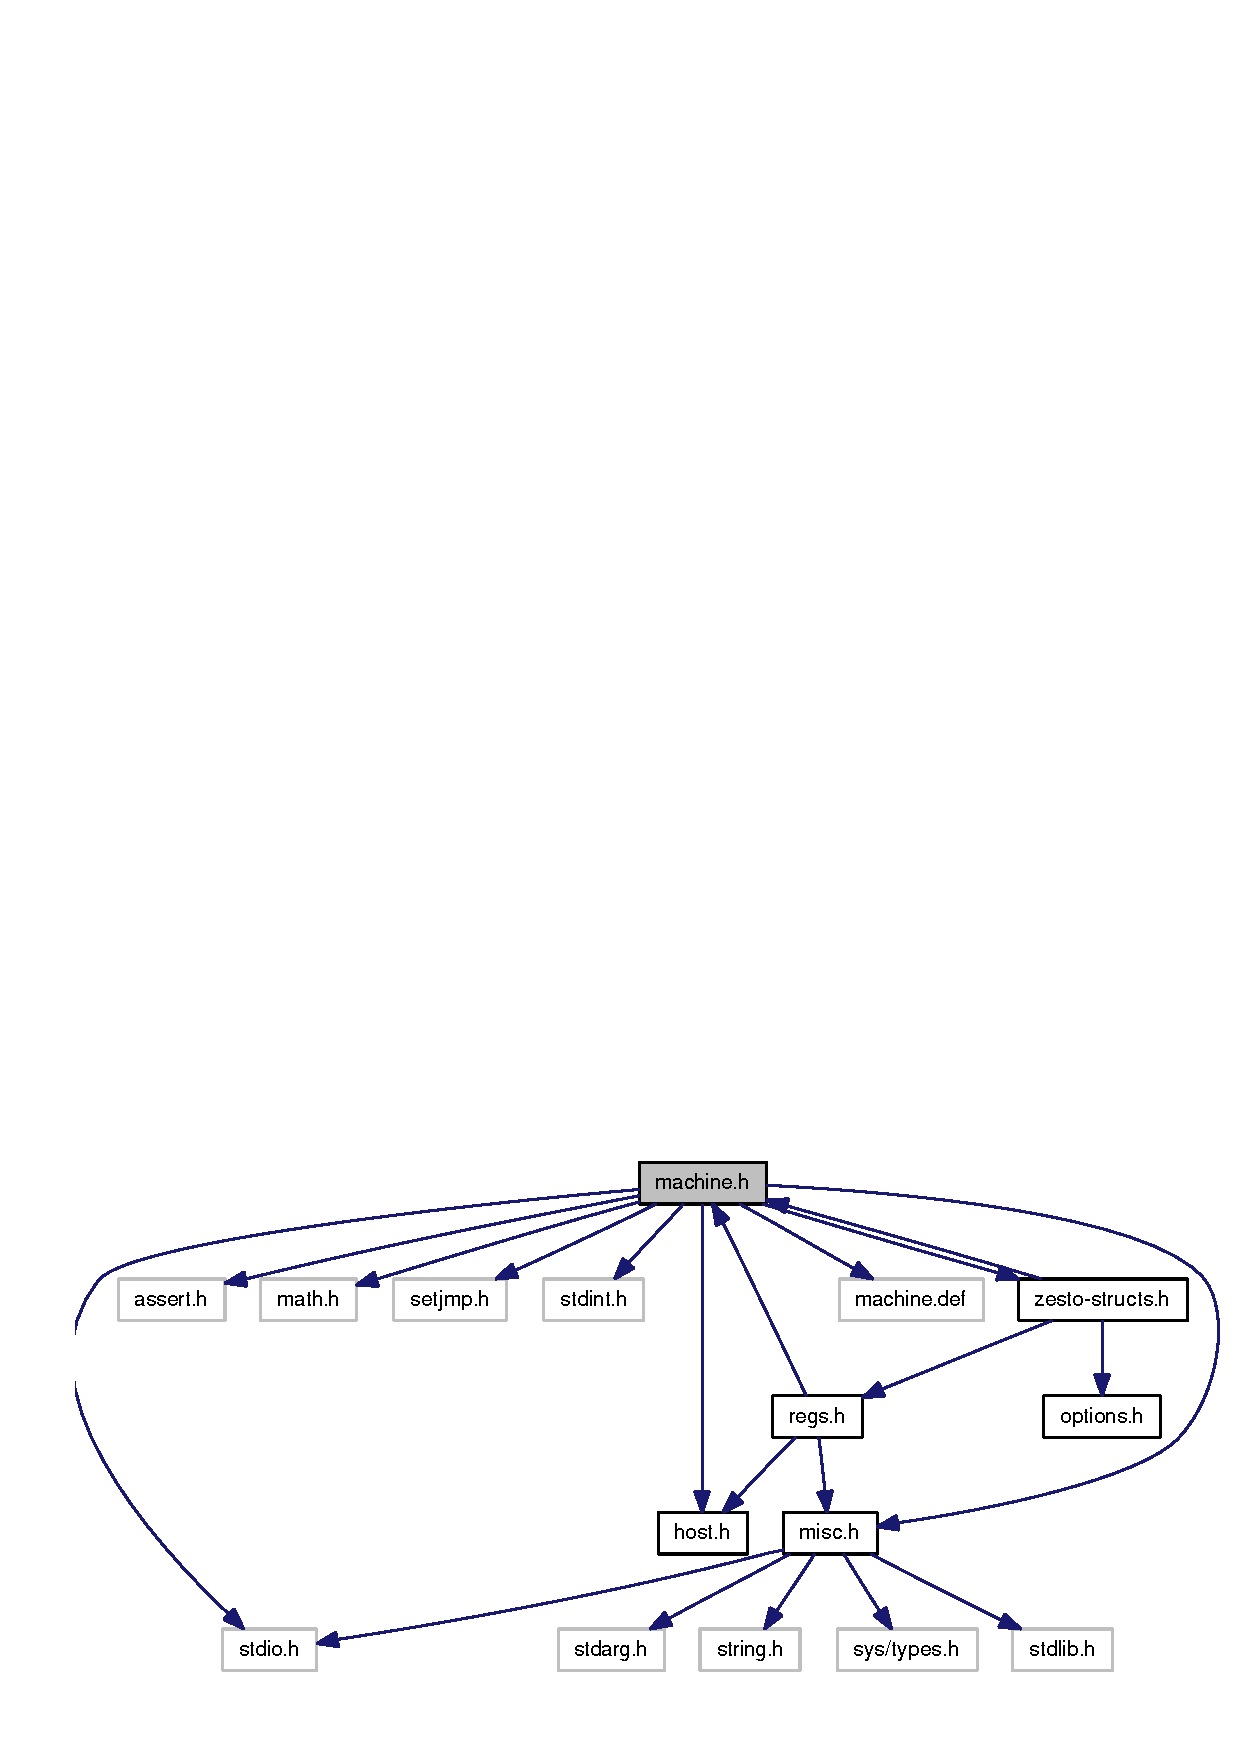
\includegraphics[width=296pt]{machine_8h__incl}
\end{center}
\end{figure}


This graph shows which files directly or indirectly include this file:\nopagebreak
\begin{figure}[H]
\begin{center}
\leavevmode
\includegraphics[width=420pt]{machine_8h__dep__incl}
\end{center}
\end{figure}
\subsection*{Classes}
\begin{CompactItemize}
\item 
union {\bf md\_\-gpr\_\-t}
\item 
union {\bf md\_\-fpr\_\-t}
\item 
union {\bf md\_\-seg\_\-t}
\item 
struct {\bf md\_\-ctrl\_\-t}
\item 
struct {\bf mem\_\-ops}
\item 
struct {\bf md\_\-inst\_\-t}
\item 
struct {\bf md\_\-reg\_\-names\_\-t}
\end{CompactItemize}
\subsection*{Defines}
\begin{CompactItemize}
\item 
\#define {\bf bool}~int
\item 
\#define {\bf TARGET\_\-X86}
\item 
\#define {\bf MAX\_\-CORES}~16
\item 
\#define {\bf NA}~0
\item 
\#define {\bf DNA}~-1
\item 
\#define {\bf MD\_\-PAGE\_\-SIZE}~4096
\item 
\#define {\bf MD\_\-LOG\_\-PAGE\_\-SIZE}~12
\item 
\#define {\bf IACOMPRESS}(A)~(A)
\item 
\#define {\bf ISCOMPRESS}(SZ)~(SZ)
\item 
\#define {\bf MD\_\-NUM\_\-IREGS}~(/$\ast$ arch $\ast$/8 + /$\ast$ uarch $\ast$/8)
\item 
\#define {\bf MD\_\-NUM\_\-ARCH\_\-IREGS}~8
\item 
\#define {\bf MD\_\-NUM\_\-FREGS}~(/$\ast$ arch $\ast$/8 + /$\ast$ uarch $\ast$/8)
\item 
\#define {\bf MD\_\-NUM\_\-CREGS}~3
\item 
\#define {\bf MD\_\-NUM\_\-SREGS}~6
\item 
\#define {\bf MD\_\-TOTAL\_\-REGS}~(/$\ast$int$\ast$/MD\_\-NUM\_\-IREGS + /$\ast$fp$\ast$/MD\_\-NUM\_\-FREGS + /$\ast$misc$\ast$/MD\_\-NUM\_\-CREGS + /$\ast$seg$\ast$/MD\_\-NUM\_\-SREGS )
\item 
\#define {\bf GPR\_\-OFFSET}~0
\item 
\#define {\bf FPR\_\-OFFSET}~MD\_\-NUM\_\-IREGS
\item 
\#define {\bf CREG\_\-OFFSET}~(FPR\_\-OFFSET+MD\_\-NUM\_\-FREGS)
\item 
\#define {\bf SEG\_\-OFFSET}~(CREG\_\-OFFSET+MD\_\-NUM\_\-CREGS)
\item 
\#define {\bf REG\_\-IS\_\-GPR}(N)~(((N) $>$= GPR\_\-OFFSET) \&\& ((N) $<$ FPR\_\-OFFSET))
\item 
\#define {\bf REG\_\-IS\_\-FPR}(N)~(((N) $>$= FPR\_\-OFFSET) \&\& ((N) $<$ CREG\_\-OFFSET))
\item 
\#define {\bf REG\_\-IS\_\-CREG}(N)~(((N) $>$= CREG\_\-OFFSET) \&\& ((N) $<$ SREG\_\-OFFSET))
\item 
\#define {\bf REG\_\-IS\_\-SEG}(N)~(((N) $>$= SEG\_\-OFFSET) \&\& ((N) $<$ MD\_\-TOTAL\_\-REGS))
\item 
\#define {\bf DGPR}(N)~((N)+GPR\_\-OFFSET)
\item 
\#define {\bf DFPR}(N)~((F2P(N))+FPR\_\-OFFSET)
\item 
\#define {\bf DCREG}(N)~((N)+CREG\_\-OFFSET)
\item 
\#define {\bf DSEG}(N)~((N)+SEG\_\-OFFSET)
\item 
\#define {\bf DGPR\_\-B}(N)~((\_\-ARCH(N) ? (\_\-ID(N)) : (N)) + GPR\_\-OFFSET)
\item 
\#define {\bf DGPR\_\-W}(N)~(N+GPR\_\-OFFSET)
\item 
\#define {\bf DGPR\_\-D}(N)~(N+GPR\_\-OFFSET)
\item 
\#define {\bf \_\-DGPR}(N)~((N)-GPR\_\-OFFSET)
\item 
\#define {\bf \_\-DFPR}(N)~((N)-FPR\_\-OFFSET)
\item 
\#define {\bf \_\-DCREG}(N)~((N)-CREG\_\-OFFSET)
\item 
\#define {\bf \_\-DSEG}(N)~((N)-SEG\_\-OFFSET)
\item 
\#define {\bf MD\_\-REG\_\-PC}~0
\item 
\#define {\bf MD\_\-MAX\_\-ILEN}~16
\item 
\#define {\bf MODE\_\-OPER32}~0x0001
\item 
\#define {\bf MODE\_\-ADDR32}~0x0002
\item 
\#define {\bf MODE\_\-STACK32}~0x0004
\item 
\#define {\bf REP\_\-NONE}~0
\item 
\#define {\bf REP\_\-REPNZ}~1
\item 
\#define {\bf REP\_\-REPZ}~2
\item 
\#define {\bf REP\_\-REP}~3
\item 
\#define {\bf SEG\_\-DEF}~0
\item 
\#define {\bf SEG\_\-CS}~1
\item 
\#define {\bf SEG\_\-SS}~2
\item 
\#define {\bf SEG\_\-DS}~3
\item 
\#define {\bf SEG\_\-ES}~4
\item 
\#define {\bf SEG\_\-FS}~5
\item 
\#define {\bf SEG\_\-GS}~6
\item 
\#define {\bf SCALE\_\-1}~0
\item 
\#define {\bf SCALE\_\-2}~1
\item 
\#define {\bf SCALE\_\-4}~2
\item 
\#define {\bf SCALE\_\-8}~3
\item 
\#define {\bf MD\_\-SWAPW}(X)~(X)
\item 
\#define {\bf MD\_\-SWAPD}(X)~(X)
\item 
\#define {\bf MD\_\-SWAPI}(X)~(X)
\item 
\#define {\bf MD\_\-SWAPQ}(X)~(X)
\item 
\#define {\bf MD\_\-INST\_\-SIZE}(INST)~(INST).len
\item 
\#define {\bf MD\_\-MAX\_\-ENVIRON}~16384
\item 
\#define {\bf DEFINST}(OP, MSK, NAME, OPFORM, RES, CLASS, O1, I1, I2, I3, OFLAGS, IFLAGS)~OP,
\item 
\#define {\bf DEFUOP}(OP, MSK, NAME, OPFORM, RES, CLASS, O1, I1, I2, I3, OFLAGS, IFLAGS)~OP,
\item 
\#define {\bf DEFLINK}(OP, MSK, NAME, MASK, SHIFT)~OP,
\item 
\#define {\bf CONNECT}(OP)
\item 
\#define {\bf MD\_\-SET\_\-OPCODE}(OP, INST)~(OP) = md\_\-decode(MODE\_\-OPER32$|$MODE\_\-ADDR32$|$MODE\_\-STACK32, \&INST, 0)
\item 
\#define {\bf MD\_\-SET\_\-OPCODE\_\-DURING\_\-FETCH}(OP, INST)~(OP) = md\_\-decode(MODE\_\-OPER32$|$MODE\_\-ADDR32$|$MODE\_\-STACK32, \&INST, 1)
\item 
\#define {\bf MD\_\-GET\_\-UOP}(FLOW, INDEX)~((uop = \&FLOW[INDEX]),MD\_\-SET\_\-UOPCODE(op,uop))
\item 
\#define {\bf MD\_\-CHECK\_\-PRED}(OP, INST)~TRUE
\item 
\#define {\bf MD\_\-INC\_\-FLOW}~(UHASIMM ? 3 : 1)
\item 
\#define {\bf MD\_\-MAX\_\-MASK}~2048
\item 
\#define {\bf MD\_\-OP\_\-NAME}(OP)~({\bf md\_\-op2name}[OP])
\item 
\#define {\bf MD\_\-OP\_\-ENUM}(OP)~({\bf md\_\-op2enum}[OP])
\item 
\#define {\bf MD\_\-OP\_\-FORMAT}(OP)~({\bf md\_\-op2format}[OP])
\item 
\#define {\bf MD\_\-OP\_\-FUCLASS}(OP)~({\bf md\_\-op2fu}[OP])
\item 
\#define {\bf MD\_\-FU\_\-NAME}(FU)~({\bf md\_\-fu2name}[FU])
\item 
\#define {\bf F\_\-ICOMP}~0x00000001
\item 
\#define {\bf F\_\-FCOMP}~0x00000002
\item 
\#define {\bf F\_\-CTRL}~0x00000004
\item 
\#define {\bf F\_\-UNCOND}~0x00000008
\item 
\#define {\bf F\_\-COND}~0x00000010
\item 
\#define {\bf F\_\-MEM}~0x00000020
\item 
\#define {\bf F\_\-LOAD}~0x00000040
\item 
\#define {\bf F\_\-STORE}~0x00000080
\item 
\#define {\bf F\_\-DISP}~0x00000100
\item 
\#define {\bf F\_\-RR}~0x00000200
\item 
\#define {\bf F\_\-DIRECT}~0x00000400
\item 
\#define {\bf F\_\-TRAP}~0x00000800
\item 
\#define {\bf F\_\-LONGLAT}~0x00001000
\item 
\#define {\bf F\_\-DIRJMP}~0x00002000
\item 
\#define {\bf F\_\-INDIRJMP}~0x00004000
\item 
\#define {\bf F\_\-CALL}~0x00008000
\item 
\#define {\bf F\_\-FPCOND}~0x00010000
\item 
\#define {\bf F\_\-IMM}~0x00020000
\item 
\#define {\bf F\_\-CISC}~0x00040000
\item 
\#define {\bf F\_\-AGEN}~0x00080000
\item 
\#define {\bf F\_\-IMMB}~0x00100000
\item 
\#define {\bf F\_\-IMMW}~0x00200000
\item 
\#define {\bf F\_\-IMMD}~0x00300000
\item 
\#define {\bf F\_\-IMMV}~0x00400000
\item 
\#define {\bf F\_\-IMMA}~0x00500000
\item 
\#define {\bf F\_\-UIMM}~0x01000000
\item 
\#define {\bf F\_\-NOMOD}~0x02000000
\item 
\#define {\bf F\_\-REP}~0x04000000
\item 
\#define {\bf F\_\-UCODE}~0x08000000
\item 
\#define {\bf F\_\-RTS}~0x10000000
\item 
\#define {\bf F\_\-SPEC}~0x20000000
\item 
\#define {\bf F\_\-RETN}~0x40000000
\item 
\#define {\bf F\_\-FENCE}~0x80000000
\item 
\#define {\bf F\_\-HASIMM}~0x00f00000
\item 
\#define {\bf F\_\-IMMSZ}(M, X)
\item 
\#define {\bf MD\_\-OP\_\-FLAGS}(OP)~({\bf md\_\-op2flags}[OP])
\item 
\#define {\bf RO}~(Mop $\rightarrow$ fetch.inst.code[Mop $\rightarrow$ fetch.inst.npfx + Mop $\rightarrow$ fetch.inst.nopc - 1] \& 0x07)
\item 
\#define {\bf R}~((Mop $\rightarrow$ fetch.inst.code[Mop $\rightarrow$ fetch.inst.npfx + Mop $\rightarrow$ fetch.inst.nopc] $>$$>$ 3) \& 0x07)
\item 
\#define {\bf RM}~(Mop $\rightarrow$ fetch.inst.code[Mop $\rightarrow$ fetch.inst.npfx + Mop $\rightarrow$ fetch.inst.nopc] \& 0x07)
\item 
\#define {\bf STI}~(Mop $\rightarrow$ fetch.inst.code[Mop $\rightarrow$ fetch.inst.npfx + Mop $\rightarrow$ fetch.inst.nopc] \& 0x07)
\item 
\#define {\bf SEG\_\-INDEX}~Mop $\rightarrow$ fetch.inst.seg-1
\item 
\#define {\bf SEG}
\item 
\#define {\bf BASE}
\item 
\#define {\bf INDEX}
\item 
\#define {\bf SCALE}~(Mop $\rightarrow$ fetch.inst.scale)
\item 
\#define {\bf DISP}~(Mop $\rightarrow$ fetch.inst.disp)
\item 
\#define {\bf AGEN\_\-W}(S, B, I, SC, D)
\item 
\#define {\bf AGEN\_\-D}(S, B, I, SC, D)
\item 
\#define {\bf AGEN\_\-A}(S, B, I, SC, D)~((Mop $\rightarrow$ fetch.inst.mode \& MODE\_\-ADDR32) ? AGEN\_\-D(S,B,I,SC,D) : AGEN\_\-W(S,B,I,SC,D))
\item 
\#define {\bf AGEN\_\-S}(S, B, I, SC, D)~((Mop $\rightarrow$ fetch.inst.mode \& MODE\_\-STACK32) ? AGEN\_\-D(S,B,I,SC,D) : AGEN\_\-W(S,B,I,SC,D))
\item 
\#define {\bf MODRM\_\-MOD}(X)~(((X) $>$$>$ 6) \& 0x03)
\item 
\#define {\bf MODRM\_\-R}(X)~(((X) $>$$>$ 3) \& 0x07)
\item 
\#define {\bf MODRM\_\-OPC}(X)~(((X) $>$$>$ 3) \& 0x07)
\item 
\#define {\bf MODRM\_\-RM}(X)~((X) \& 0x07)
\item 
\#define {\bf SIB\_\-SCALE}(X)~(((X) $>$$>$ 6) \& 0x03)
\item 
\#define {\bf SIB\_\-INDEX}(X)~(((X) $>$$>$ 3) \& 0x07)
\item 
\#define {\bf SIB\_\-BASE}(X)~((X) \& 0x07)
\item 
\#define {\bf CC}~(Mop $\rightarrow$ fetch.inst.code[Mop $\rightarrow$ fetch.inst.npfx + Mop $\rightarrow$ fetch.inst.nopc - 1] \& 0x0f)
\item 
\#define {\bf LC}~(Mop $\rightarrow$ fetch.inst.code[Mop $\rightarrow$ fetch.inst.npfx + Mop $\rightarrow$ fetch.inst.nopc] \& 0x07)
\item 
\#define {\bf IMM\_\-B}~(assert(Mop $\rightarrow$ fetch.inst.nimm == 1), Mop $\rightarrow$ fetch.inst.imm)
\item 
\#define {\bf IMM\_\-W}~(assert(Mop $\rightarrow$ fetch.inst.nimm == 2), Mop $\rightarrow$ fetch.inst.imm)
\item 
\#define {\bf IMM\_\-D}~(assert(Mop $\rightarrow$ fetch.inst.nimm == 4), Mop $\rightarrow$ fetch.inst.imm)
\item 
\#define {\bf IMM\_\-V}
\item 
\#define {\bf IMM\_\-A}
\item 
\#define {\bf UIMM\_\-B}~(assert(Mop $\rightarrow$ fetch.inst.nimm == 1), ({\bf dword\_\-t})(Mop $\rightarrow$ fetch.inst.imm \& 0xff))
\item 
\#define {\bf UIMM\_\-W}~(assert(Mop $\rightarrow$ fetch.inst.nimm == 2), ({\bf dword\_\-t})(Mop $\rightarrow$ fetch.inst.imm \& 0xffff))
\item 
\#define {\bf UIMM\_\-D}~(assert(Mop $\rightarrow$ fetch.inst.nimm == 4), ({\bf dword\_\-t})Mop $\rightarrow$ fetch.inst.imm)
\item 
\#define {\bf UIMM\_\-V}
\item 
\#define {\bf UIMM\_\-A}
\item 
\#define {\bf OFS}~(({\bf dword\_\-t})(Mop $\rightarrow$ fetch.inst \& 0xfff))
\item 
\#define {\bf HOFS}~(({\bf dword\_\-t})((RS $<$$<$ 4) + RM))
\item 
\#define {\bf FPOFS}~(({\bf dword\_\-t})((Mop $\rightarrow$ fetch.inst \& 0xff) $<$$<$ 2))
\item 
\#define {\bf BOFS}
\item 
\#define {\bf IS\_\-EVEN\_\-ONES}(r)
\item 
\#define {\bf CPOPC}~((Mop $\rightarrow$ fetch.inst $>$$>$ 20) \& 0x0f)
\item 
\#define {\bf CPEXT}~((Mop $\rightarrow$ fetch.inst $>$$>$ 5) \& 0x07)
\item 
\#define {\bf MD\_\-MAX\_\-FLAGS}~12
\item 
\#define {\bf CF}~0x00000001
\item 
\#define {\bf PF}~0x00000004
\item 
\#define {\bf AF}~0x00000010
\item 
\#define {\bf ZF}~0x00000040
\item 
\#define {\bf SF}~0x00000080
\item 
\#define {\bf DF}~0x00000400
\item 
\#define {\bf OF}~0x00000800
\item 
\#define {\bf MKCF}(X)~((!!(X)) $<$$<$ 0)
\item 
\#define {\bf MKPF}(X)~((!!(X)) $<$$<$ 2)
\item 
\#define {\bf MKAF}(X)~((!!(X)) $<$$<$ 4)
\item 
\#define {\bf MKZF}(X)~((!!(X)) $<$$<$ 6)
\item 
\#define {\bf MKSF}(X)~((!!(X)) $<$$<$ 7)
\item 
\#define {\bf MKDF}(X)~((!!(X)) $<$$<$ 10)
\item 
\#define {\bf MKOF}(X)~((!!(X)) $<$$<$ 11)
\item 
\#define {\bf IE}~0x0001
\item 
\#define {\bf DE}~0x0002
\item 
\#define {\bf ZE}~0x0004
\item 
\#define {\bf OE}~0x0008
\item 
\#define {\bf UE}~0x0010
\item 
\#define {\bf PE}~0x0020
\item 
\#define {\bf FSF}~0x0040
\item 
\#define {\bf ES}~0x0080
\item 
\#define {\bf C0}~0x0100
\item 
\#define {\bf C1}~0x0200
\item 
\#define {\bf C2}~0x0400
\item 
\#define {\bf C3}~0x4000
\item 
\#define {\bf MKIE}(X)~((!!(X)) $<$$<$ 0)
\item 
\#define {\bf MKDE}(X)~((!!(X)) $<$$<$ 1)
\item 
\#define {\bf MKZE}(X)~((!!(X)) $<$$<$ 2)
\item 
\#define {\bf MKOE}(X)~((!!(X)) $<$$<$ 3)
\item 
\#define {\bf MKUE}(X)~((!!(X)) $<$$<$ 4)
\item 
\#define {\bf MKPE}(X)~((!!(X)) $<$$<$ 5)
\item 
\#define {\bf MKFSF}(X)~((!!(X)) $<$$<$ 6)
\item 
\#define {\bf MKES}(X)~((!!(X)) $<$$<$ 7)
\item 
\#define {\bf MKC0}(X)~((!!(X)) $<$$<$ 8)
\item 
\#define {\bf MKC1}(X)~((!!(X)) $<$$<$ 9)
\item 
\#define {\bf MKC2}(X)~((!!(X)) $<$$<$ 10)
\item 
\#define {\bf MKC3}(X)~((!!(X)) $<$$<$ 14)
\item 
\#define {\bf FSW\_\-TOP}(X)~(((X) $>$$>$ 11) \& 0x07)
\item 
\#define {\bf SET\_\-FSW\_\-TOP}(X, N)~((X) = (((X) \& $\sim$(7$<$$<$11)) $|$ (((N) \& 7)$<$$<$11)))
\item 
\#define {\bf IM}~0x0001
\item 
\#define {\bf DM}~0x0002
\item 
\#define {\bf ZM}~0x0004
\item 
\#define {\bf OM}~0x0008
\item 
\#define {\bf UM}~0x0010
\item 
\#define {\bf PM}~0x0020
\item 
\#define {\bf UNDEF}~0
\item 
\#define {\bf MUL\_\-B}(S1, S2)~(({\bf word\_\-t})(S1) $\ast$ ({\bf word\_\-t})(S2))
\item 
\#define {\bf AFLAGS\_\-MULB}(R)
\item 
\#define {\bf MULHI\_\-W}(S1, S2)~(({\bf word\_\-t})((({\bf dword\_\-t})({\bf word\_\-t})(S1) $\ast$ ({\bf dword\_\-t})({\bf word\_\-t})(S2)) $>$$>$ 16))
\item 
\#define {\bf MULHI\_\-D}(S1, S2)~(({\bf dword\_\-t})(((qword\_\-t)({\bf dword\_\-t})(S1) $\ast$ (qword\_\-t)({\bf dword\_\-t})(S2)) $>$$>$ 32))
\item 
\#define {\bf MULLO\_\-W}(S1, S2)~(({\bf word\_\-t})(({\bf dword\_\-t})({\bf word\_\-t})(S1) $\ast$ ({\bf dword\_\-t})({\bf word\_\-t})(S2)))
\item 
\#define {\bf MULLO\_\-D}(S1, S2)~(({\bf dword\_\-t})((qword\_\-t)({\bf dword\_\-t})(S1) $\ast$ (qword\_\-t)({\bf dword\_\-t})(S2)))
\item 
\#define {\bf AFLAGS\_\-MULW}(RHI)~(((RHI) != 0) ? (MKOF(1)$|$MKCF(1)) : (MKOF(0)$|$MKCF(0)))
\item 
\#define {\bf AFLAGS\_\-MULD}(RHI)~(((RHI) != 0) ? (MKOF(1)$|$MKCF(1)) : (MKOF(0)$|$MKCF(0)))
\item 
\#define {\bf MULHI\_\-V}(S1, S2)~((Mop $\rightarrow$ fetch.inst.mode \& MODE\_\-OPER32) ? MULHI\_\-D(S1,S2) : MULHI\_\-W(S1,S2))
\item 
\#define {\bf MULLO\_\-V}(S1, S2)~((Mop $\rightarrow$ fetch.inst.mode \& MODE\_\-OPER32) ? MULLO\_\-D(S1,S2) : MULLO\_\-W(S1,S2))
\item 
\#define {\bf AFLAGS\_\-MULV}(RHI)~(((RHI) != 0) ? (MKOF(1)$|$MKCF(1)) : (MKOF(0)$|$MKCF(0)))
\item 
\#define {\bf IMUL\_\-B}(S1, S2)~(({\bf sword\_\-t})({\bf sbyte\_\-t})(S1) $\ast$ ({\bf sword\_\-t})({\bf sbyte\_\-t})(S2))
\item 
\#define {\bf AFLAGS\_\-IMULB}(R, S1, S2)
\item 
\#define {\bf IMUL\_\-W}(S1, S2)~(({\bf sword\_\-t})(S1) $\ast$ ({\bf sword\_\-t})(S2))
\item 
\#define {\bf IMUL\_\-D}(S1, S2)~(({\bf sdword\_\-t})(S1) $\ast$ ({\bf sdword\_\-t})(S2))
\item 
\#define {\bf AFLAGS\_\-IMULW}(R, S1, S2)
\item 
\#define {\bf AFLAGS\_\-IMULD}(R, S1, S2)
\item 
\#define {\bf IMUL\_\-V}(S1, S2)~((Mop $\rightarrow$ fetch.inst.mode \& MODE\_\-OPER32) ? IMUL\_\-D(S1,S2) : IMUL\_\-W(S1,S2))
\item 
\#define {\bf AFLAGS\_\-IMULV}(R, S1, S2)~((Mop $\rightarrow$ fetch.inst.mode \& MODE\_\-OPER32) ? AFLAGS\_\-IMULD(R,S1,S2) : AFLAGS\_\-IMULW(R,S1,S2))
\item 
\#define {\bf IMULHI\_\-W}(S1, S2)~(({\bf word\_\-t})((({\bf sdword\_\-t})({\bf sword\_\-t})(S1) $\ast$ ({\bf sdword\_\-t})({\bf sword\_\-t})(S2)) $>$$>$ 16))
\item 
\#define {\bf IMULHI\_\-D}(S1, S2)~(({\bf dword\_\-t})(((sqword\_\-t)({\bf sdword\_\-t})(S1) $\ast$ (sqword\_\-t)({\bf sdword\_\-t})(S2)) $>$$>$ 32))
\item 
\#define {\bf IMULLO\_\-W}(S1, S2)~(({\bf word\_\-t})(({\bf sdword\_\-t})({\bf sword\_\-t})(S1) $\ast$ ({\bf sdword\_\-t})({\bf sword\_\-t})(S2)))
\item 
\#define {\bf IMULLO\_\-D}(S1, S2)~(({\bf dword\_\-t})((sqword\_\-t)({\bf sdword\_\-t})(S1) $\ast$ (sqword\_\-t)({\bf sdword\_\-t})(S2)))
\item 
\#define {\bf IMULHI\_\-V}(S1, S2)~((Mop $\rightarrow$ fetch.inst.mode \& MODE\_\-OPER32) ? IMULHI\_\-D(S1,S2) : IMULHI\_\-W(S1,S2))
\item 
\#define {\bf IMULLO\_\-V}(S1, S2)~((Mop $\rightarrow$ fetch.inst.mode \& MODE\_\-OPER32) ? IMULLO\_\-D(S1,S2) : IMULLO\_\-W(S1,S2))
\item 
\#define {\bf AFLAGS\_\-IMULHIV}(RHI, RLO)
\item 
\#define {\bf AFLAGS\_\-IMULHIW}(RHI, RLO)
\item 
\#define {\bf AFLAGS\_\-IMULHID}(RHI, RLO)
\item 
\#define {\bf QUO\_\-B}(S1, S2)~(({\bf byte\_\-t})(({\bf word\_\-t})(S1) / ({\bf byte\_\-t})(S2)))
\item 
\#define {\bf REM\_\-B}(S1, S2)~(({\bf byte\_\-t})(({\bf word\_\-t})(S1) \% ({\bf byte\_\-t})(S2)))
\item 
\#define {\bf AFLAGS\_\-DIVB}()~(UNDEF)
\item 
\#define {\bf QUO\_\-W}(S1H, S1L, S2)
\item 
\#define {\bf QUO\_\-D}(S1H, S1L, S2)
\item 
\#define {\bf REM\_\-W}(S1H, S1L, S2)
\item 
\#define {\bf REM\_\-D}(S1H, S1L, S2)
\item 
\#define {\bf AFLAGS\_\-DIVW}()~(UNDEF)
\item 
\#define {\bf AFLAGS\_\-DIVD}()~(UNDEF)
\item 
\#define {\bf QUO\_\-V}(S1H, S1L, S2)~((Mop $\rightarrow$ fetch.inst.mode \& MODE\_\-OPER32) ? QUO\_\-D(S1H,S1L,S2) : QUO\_\-W(S1H,S1L,S2))
\item 
\#define {\bf REM\_\-V}(S1H, S1L, S2)~((Mop $\rightarrow$ fetch.inst.mode \& MODE\_\-OPER32) ? REM\_\-D(S1H,S1L,S2) : REM\_\-W(S1H,S1L,S2))
\item 
\#define {\bf AFLAGS\_\-DIVV}()~(UNDEF)
\item 
\#define {\bf IQUO\_\-B}(S1, S2)~(({\bf sbyte\_\-t})(({\bf sword\_\-t})(S1) / ({\bf sbyte\_\-t})(S2)))
\item 
\#define {\bf IREM\_\-B}(S1, S2)~(({\bf sbyte\_\-t})(({\bf sword\_\-t})(S1) \% ({\bf sbyte\_\-t})(S2)))
\item 
\#define {\bf AFLAGS\_\-IDIVB}()~(UNDEF)
\item 
\#define {\bf IQUO\_\-W}(S1H, S1L, S2)
\item 
\#define {\bf IQUO\_\-D}(S1H, S1L, S2)
\item 
\#define {\bf IREM\_\-W}(S1H, S1L, S2)
\item 
\#define {\bf IREM\_\-D}(S1H, S1L, S2)
\item 
\#define {\bf AFLAGS\_\-IDIVW}()~(UNDEF)
\item 
\#define {\bf AFLAGS\_\-IDIVD}()~(UNDEF)
\item 
\#define {\bf IQUO\_\-V}(S1H, S1L, S2)~((Mop $\rightarrow$ fetch.inst.mode \& MODE\_\-OPER32) ? IQUO\_\-D(S1H,S1L,S2) : IQUO\_\-W(S1H,S1L,S2))
\item 
\#define {\bf IREM\_\-V}(S1H, S1L, S2)~((Mop $\rightarrow$ fetch.inst.mode \& MODE\_\-OPER32) ? IREM\_\-D(S1H,S1L,S2) : IREM\_\-W(S1H,S1L,S2))
\item 
\#define {\bf AFLAGS\_\-IDIVV}()~(UNDEF)
\item 
\#define {\bf AFLAGS\_\-ADDB}(R, S1, S2)
\item 
\#define {\bf AFLAGS\_\-ADDW}(R, S1, S2)
\item 
\#define {\bf AFLAGS\_\-ADDD}(R, S1, S2)
\item 
\#define {\bf AFLAGS\_\-ADDV}(R, S1, S2)~((Mop $\rightarrow$ fetch.inst.mode \& MODE\_\-OPER32) ? AFLAGS\_\-ADDD(R, S1, S2) : AFLAGS\_\-ADDW(R, S1, S2))
\item 
\#define {\bf AFLAGS\_\-SUBB}(R, S1, S2)
\item 
\#define {\bf AFLAGS\_\-SUBW}(R, S1, S2)
\item 
\#define {\bf AFLAGS\_\-SUBD}(R, S1, S2)
\item 
\#define {\bf AFLAGS\_\-SUBV}(R, S1, S2)~((Mop $\rightarrow$ fetch.inst.mode \& MODE\_\-OPER32) ? AFLAGS\_\-SUBD(R, S1, S2) : AFLAGS\_\-SUBW(R, S1, S2))
\item 
\#define {\bf AFLAGS\_\-ALUB}(R)
\item 
\#define {\bf AFLAGS\_\-ALUW}(R)
\item 
\#define {\bf AFLAGS\_\-ALUD}(R)
\item 
\#define {\bf AFLAGS\_\-ALUV}(R)~((Mop $\rightarrow$ fetch.inst.mode \& MODE\_\-OPER32) ? AFLAGS\_\-ALUD(R) : AFLAGS\_\-ALUW(R))
\item 
\#define {\bf AFLAGS\_\-INCB}(R)
\item 
\#define {\bf AFLAGS\_\-INCW}(R)
\item 
\#define {\bf AFLAGS\_\-INCD}(R)
\item 
\#define {\bf AFLAGS\_\-INCV}(R)~((Mop $\rightarrow$ fetch.inst.mode \& MODE\_\-OPER32) ? AFLAGS\_\-INCD(R) : AFLAGS\_\-INCW(R))
\item 
\#define {\bf AFLAGS\_\-DECB}(R)
\item 
\#define {\bf AFLAGS\_\-DECW}(R)
\item 
\#define {\bf AFLAGS\_\-DECD}(R)
\item 
\#define {\bf AFLAGS\_\-DECV}(R)~((Mop $\rightarrow$ fetch.inst.mode \& MODE\_\-OPER32) ? AFLAGS\_\-DECD(R) : AFLAGS\_\-DECW(R))
\item 
\#define {\bf AFLAGS\_\-ADCB}(R, S1, S2, C)
\item 
\#define {\bf AFLAGS\_\-ADCW}(R, S1, S2, C)
\item 
\#define {\bf AFLAGS\_\-ADCD}(R, S1, S2, C)
\item 
\#define {\bf AFLAGS\_\-ADCV}(R, S1, S2, C)
\item 
\#define {\bf AFLAGS\_\-SBBB}(R, S1, S2, C)
\item 
\#define {\bf AFLAGS\_\-SBBW}(R, S1, S2, C)
\item 
\#define {\bf AFLAGS\_\-SBBD}(R, S1, S2, C)
\item 
\#define {\bf AFLAGS\_\-SBBV}(R, S1, S2, C)
\item 
\#define {\bf AFLAGS\_\-NEGB}(R, S)
\item 
\#define {\bf AFLAGS\_\-NEGW}(R, S)
\item 
\#define {\bf AFLAGS\_\-NEGD}(R, S)
\item 
\#define {\bf AFLAGS\_\-NEGV}(R, S)~((Mop $\rightarrow$ fetch.inst.mode \& MODE\_\-OPER32) ? AFLAGS\_\-NEGD(R,S) : AFLAGS\_\-NEGW(R,S))
\item 
\#define {\bf ROL\_\-B}(X, N)~(((X) $<$$<$ (N)) $|$ ((X) $>$$>$ (8-(N))))
\item 
\#define {\bf AFLAGS\_\-ROLB}(R, S, N)
\item 
\#define {\bf ROL\_\-W}(X, N)~(((X) $<$$<$ (N)) $|$ ((X) $>$$>$ (16-(N))))
\item 
\#define {\bf AFLAGS\_\-ROLW}(R, S, N)
\item 
\#define {\bf ROL\_\-D}(X, N)~(((X) $<$$<$ (N)) $|$ ((X) $>$$>$ (32-(N))))
\item 
\#define {\bf AFLAGS\_\-ROLD}(R, S, N)
\item 
\#define {\bf ROL\_\-V}(X, N)~((Mop $\rightarrow$ fetch.inst.mode \& MODE\_\-OPER32) ? ROL\_\-D(X,N) : ROL\_\-W(X,N))
\item 
\#define {\bf AFLAGS\_\-ROLV}(R, S, N)~((Mop $\rightarrow$ fetch.inst.mode \& MODE\_\-OPER32) ? AFLAGS\_\-ROLD(R,S,N) : AFLAGS\_\-ROLW(R,S,N))
\item 
\#define {\bf ROR\_\-B}(X, N)~(((X) $>$$>$ (N)) $|$ ((X) $<$$<$ (8-(N))))
\item 
\#define {\bf AFLAGS\_\-RORB}(R, S, N)
\item 
\#define {\bf ROR\_\-W}(X, N)~(((X) $>$$>$ (N)) $|$ ((X) $<$$<$ (16-(N))))
\item 
\#define {\bf AFLAGS\_\-RORW}(R, S, N)
\item 
\#define {\bf ROR\_\-D}(X, N)~(((X) $>$$>$ (N)) $|$ ((X) $<$$<$ (32-(N))))
\item 
\#define {\bf AFLAGS\_\-RORD}(R, S, N)
\item 
\#define {\bf ROR\_\-V}(X, N)~((Mop $\rightarrow$ fetch.inst.mode \& MODE\_\-OPER32) ? ROR\_\-D(X,N) : ROR\_\-W(X,N))
\item 
\#define {\bf AFLAGS\_\-RORV}(R, S, N)~((Mop $\rightarrow$ fetch.inst.mode \& MODE\_\-OPER32) ? AFLAGS\_\-RORD(R,S,N) : AFLAGS\_\-RORW(R,S,N))
\item 
\#define {\bf RCL\_\-B}(X, CF, N)
\item 
\#define {\bf AFLAGS\_\-RCLB}(R, S, N)
\item 
\#define {\bf RCL\_\-W}(X, CF, N)
\item 
\#define {\bf AFLAGS\_\-RCLW}(R, S, N)
\item 
\#define {\bf RCL\_\-D}(X, CF, N)
\item 
\#define {\bf AFLAGS\_\-RCLD}(R, S, N)
\item 
\#define {\bf RCL\_\-V}(X, CF, N)~((Mop $\rightarrow$ fetch.inst.mode \& MODE\_\-OPER32) ? RCL\_\-D(X,CF,N) : RCL\_\-W(X,CF,N))
\item 
\#define {\bf AFLAGS\_\-RCLV}(R, S, N)~((Mop $\rightarrow$ fetch.inst.mode \& MODE\_\-OPER32) ? AFLAGS\_\-RCLD(R,S,N) : AFLAGS\_\-RCLW(R,S,N))
\item 
\#define {\bf RCR\_\-B}(X, CF, N)
\item 
\#define {\bf AFLAGS\_\-RCRB}(R, S, N)
\item 
\#define {\bf RCR\_\-W}(X, CF, N)
\item 
\#define {\bf AFLAGS\_\-RCRW}(R, S, N)
\item 
\#define {\bf RCR\_\-D}(X, CF, N)
\item 
\#define {\bf AFLAGS\_\-RCRD}(R, S, N)
\item 
\#define {\bf RCR\_\-V}(X, CF, N)~((Mop $\rightarrow$ fetch.inst.mode \& MODE\_\-OPER32) ? RCR\_\-D(X,CF,N) : RCR\_\-W(X,CF,N))
\item 
\#define {\bf AFLAGS\_\-RCRV}(R, S, N)~((Mop $\rightarrow$ fetch.inst.mode \& MODE\_\-OPER32) ? AFLAGS\_\-RCRD(R,S,N) : AFLAGS\_\-RCRW(R,S,N))
\item 
\#define {\bf SHL\_\-B}(X, N)~((X) $<$$<$ (N))
\item 
\#define {\bf AFLAGS\_\-SHLB}(R, S, N)
\item 
\#define {\bf SHL\_\-W}(X, N)~((X) $<$$<$ (N))
\item 
\#define {\bf AFLAGS\_\-SHLW}(R, S, N)
\item 
\#define {\bf SHL\_\-D}(X, N)~((X) $<$$<$ (N))
\item 
\#define {\bf AFLAGS\_\-SHLD}(R, S, N)
\item 
\#define {\bf SHL\_\-V}(X, N)~((Mop $\rightarrow$ fetch.inst.mode \& MODE\_\-OPER32) ? SHL\_\-D(X,N) : SHL\_\-W(X,N))
\item 
\#define {\bf AFLAGS\_\-SHLV}(R, S, N)~((Mop $\rightarrow$ fetch.inst.mode \& MODE\_\-OPER32) ? AFLAGS\_\-SHLD(R,S,N) : AFLAGS\_\-SHLW(R,S,N))
\item 
\#define {\bf SHR\_\-B}(X, N)~((X) $>$$>$ (N))
\item 
\#define {\bf AFLAGS\_\-SHRB}(R, S, N)
\item 
\#define {\bf SHR\_\-W}(X, N)~((X) $>$$>$ (N))
\item 
\#define {\bf AFLAGS\_\-SHRW}(R, S, N)
\item 
\#define {\bf SHR\_\-D}(X, N)~((X) $>$$>$ (N))
\item 
\#define {\bf AFLAGS\_\-SHRD}(R, S, N)
\item 
\#define {\bf SHR\_\-V}(X, N)~((Mop $\rightarrow$ fetch.inst.mode \& MODE\_\-OPER32) ? SHR\_\-D(X,N) : SHR\_\-W(X,N))
\item 
\#define {\bf AFLAGS\_\-SHRV}(R, S, N)~((Mop $\rightarrow$ fetch.inst.mode \& MODE\_\-OPER32) ? AFLAGS\_\-SHRD(R,S,N) : AFLAGS\_\-SHRW(R,S,N))
\item 
\#define {\bf SAR\_\-B}(X, N)
\item 
\#define {\bf AFLAGS\_\-SARB}(R, S, N)
\item 
\#define {\bf SAR\_\-W}(X, N)
\item 
\#define {\bf AFLAGS\_\-SARW}(R, S, N)
\item 
\#define {\bf SAR\_\-D}(X, N)
\item 
\#define {\bf AFLAGS\_\-SARD}(R, S, N)
\item 
\#define {\bf SAR\_\-V}(X, N)~((Mop $\rightarrow$ fetch.inst.mode \& MODE\_\-OPER32) ? SAR\_\-D(X,N) : SAR\_\-W(X,N))
\item 
\#define {\bf AFLAGS\_\-SARV}(R, S, N)~((Mop $\rightarrow$ fetch.inst.mode \& MODE\_\-OPER32) ? AFLAGS\_\-SARD(R,S,N) : AFLAGS\_\-SARW(R,S,N))
\item 
\#define {\bf AFLAGS\_\-SHLDD}(R, S, N)
\item 
\#define {\bf AFLAGS\_\-SHLDW}(R, S, N)
\item 
\#define {\bf AFLAGS\_\-SHLDV}(R, S, N)~((Mop $\rightarrow$ fetch.inst.mode \& MODE\_\-OPER32) ? AFLAGS\_\-SHLDD(R,S,N) : AFLAGS\_\-SHLDW(R,S,N))
\item 
\#define {\bf AFLAGS\_\-SHRDD}(R, S, N)
\item 
\#define {\bf AFLAGS\_\-SHRDW}(R, S, N)
\item 
\#define {\bf AFLAGS\_\-SHRDV}(R, S, N)~((Mop $\rightarrow$ fetch.inst.mode \& MODE\_\-OPER32) ? AFLAGS\_\-SHRDD(R,S,N) : AFLAGS\_\-SHRDW(R,S,N))
\item 
\#define {\bf BSWAP}(X)
\item 
\#define {\bf BTS\_\-V}(X, N)~((X) $|$ (1 $<$$<$ (N)))
\item 
\#define {\bf BTR\_\-V}(X, N)~((X) \& $\sim$(({\bf dword\_\-t})1 $<$$<$ (N)))
\item 
\#define {\bf BTC\_\-V}(X, N)~((X) $^\wedge$ (1 $<$$<$ (N)))
\item 
\#define {\bf AFLAGS\_\-BTV}(X, N)~MKCF(((X) $>$$>$ (N)) \& 0x01)
\item 
\#define {\bf MOVZX\_\-WB}(S)~(({\bf word\_\-t})({\bf byte\_\-t})(S))
\item 
\#define {\bf MOVZX\_\-DB}(S)~(({\bf dword\_\-t})({\bf byte\_\-t})(S))
\item 
\#define {\bf MOVZX\_\-WW}(S)~(({\bf word\_\-t})(S))
\item 
\#define {\bf MOVZX\_\-DW}(S)~(({\bf dword\_\-t})({\bf word\_\-t})(S))
\item 
\#define {\bf MOVZX\_\-VB}(S)~((Mop $\rightarrow$ fetch.inst.mode \& MODE\_\-OPER32) ? MOVZX\_\-DB(S) : MOVZX\_\-WB(S))
\item 
\#define {\bf MOVZX\_\-VW}(S)~((Mop $\rightarrow$ fetch.inst.mode \& MODE\_\-OPER32) ? MOVZX\_\-DW(S) : MOVZX\_\-WW(S))
\item 
\#define {\bf MOVSX\_\-WB}(S)~(({\bf sword\_\-t})({\bf sbyte\_\-t})(S))
\item 
\#define {\bf MOVSX\_\-DB}(S)~(({\bf sdword\_\-t})({\bf sbyte\_\-t})(S))
\item 
\#define {\bf MOVSX\_\-WW}(S)~(({\bf sword\_\-t})(S))
\item 
\#define {\bf MOVSX\_\-DW}(S)~(({\bf sdword\_\-t})({\bf sword\_\-t})(S))
\item 
\#define {\bf MOVSX\_\-VB}(S)~((Mop $\rightarrow$ fetch.inst.mode \& MODE\_\-OPER32) ? MOVSX\_\-DB(S) : MOVSX\_\-WB(S))
\item 
\#define {\bf MOVSX\_\-VW}(S)~((Mop $\rightarrow$ fetch.inst.mode \& MODE\_\-OPER32) ? MOVSX\_\-DW(S) : MOVSX\_\-WW(S))
\item 
\#define {\bf BSF\_\-W}(S)~BSF\_\-V(S)
\item 
\#define {\bf BSF\_\-D}(S)~BSF\_\-V(S)
\item 
\#define {\bf BSF\_\-V}(S)
\item 
\#define {\bf AFLAGS\_\-BSFW}(S)~MKZF(({\bf word\_\-t})(S) == 0)
\item 
\#define {\bf AFLAGS\_\-BSFD}(S)~MKZF(({\bf dword\_\-t})(S) == 0)
\item 
\#define {\bf AFLAGS\_\-BSFV}(S)~((Mop $\rightarrow$ fetch.inst.mode \& MODE\_\-OPER32) ? AFLAGS\_\-BSFD(S) : AFLAGS\_\-BSFW(S))
\item 
\#define {\bf BSR\_\-W}(S)
\item 
\#define {\bf BSR\_\-D}(S)
\item 
\#define {\bf BSR\_\-V}(S)
\item 
\#define {\bf AFLAGS\_\-BSRW}(S)~MKZF(({\bf word\_\-t})(S) == 0)
\item 
\#define {\bf AFLAGS\_\-BSRD}(S)~MKZF(({\bf dword\_\-t})(S) == 0)
\item 
\#define {\bf AFLAGS\_\-BSRV}(S)~((Mop $\rightarrow$ fetch.inst.mode \& MODE\_\-OPER32) ? AFLAGS\_\-BSRD(S) : AFLAGS\_\-BSRW(S))
\item 
\#define {\bf FSW\_\-FCOM}(S1, S2)
\item 
\#define {\bf FSW\_\-FUCOM}(S1, S2)
\item 
\#define {\bf AFLAGS\_\-FCOMI}(S1, S2)
\item 
\#define {\bf AFLAGS\_\-FUCOMI}(S1, S2)
\item 
\#define {\bf FPCONST}(LC)
\item 
\#define {\bf CC\_\-O}~0
\item 
\#define {\bf CC\_\-NO}~1
\item 
\#define {\bf CC\_\-B}~2
\item 
\#define {\bf CC\_\-NB}~3
\item 
\#define {\bf CC\_\-E}~4
\item 
\#define {\bf CC\_\-NE}~5
\item 
\#define {\bf CC\_\-BE}~6
\item 
\#define {\bf CC\_\-NBE}~7
\item 
\#define {\bf CC\_\-S}~8
\item 
\#define {\bf CC\_\-NS}~9
\item 
\#define {\bf CC\_\-P}~10
\item 
\#define {\bf CC\_\-NP}~11
\item 
\#define {\bf CC\_\-L}~12
\item 
\#define {\bf CC\_\-NL}~13
\item 
\#define {\bf CC\_\-LE}~14
\item 
\#define {\bf CC\_\-NLE}~15
\item 
\#define {\bf CC\_\-EVAL}(CC, F)~md\_\-cc\_\-eval(CC, F, bogus)
\item 
\#define {\bf FCC\_\-B}~0
\item 
\#define {\bf FCC\_\-E}~1
\item 
\#define {\bf FCC\_\-BE}~2
\item 
\#define {\bf FCC\_\-U}~3
\item 
\#define {\bf FCC\_\-NB}~4
\item 
\#define {\bf FCC\_\-NE}~5
\item 
\#define {\bf FCC\_\-NBE}~6
\item 
\#define {\bf FCC\_\-NU}~7
\item 
\#define {\bf FCC\_\-EVAL}(FCC, F)~md\_\-fcc\_\-eval(FCC, F, bogus)
\item 
\#define {\bf SIZE\_\-V}~((Mop $\rightarrow$ fetch.inst.mode \& MODE\_\-OPER32) ? 4 : 2)
\item 
\#define {\bf BITSIZE\_\-V}~((Mop $\rightarrow$ fetch.inst.mode \& MODE\_\-OPER32) ? 32 : 16)
\item 
\#define {\bf LOGSIZE\_\-V}~((Mop $\rightarrow$ fetch.inst.mode \& MODE\_\-OPER32) ? 2 : 1)
\item 
\#define {\bf LOGBITSIZE\_\-V}~((Mop $\rightarrow$ fetch.inst.mode \& MODE\_\-OPER32) ? 5 : 4)
\item 
\#define {\bf SIGN\_\-V}(X)
\item 
\#define {\bf QW2E}(S1, S2)
\item 
\#define {\bf E2Qw}(E)
\item 
\#define {\bf E2qW}(E)
\item 
\#define {\bf SET\_\-TPC}(PC)~Mop $\rightarrow$ decode.targetPC = (PC)
\item 
\#define {\bf SET\_\-TPC\_\-D}(PC)~Mop $\rightarrow$ decode.targetPC = (PC)
\item 
\#define {\bf SET\_\-TPC\_\-V}(PC)~Mop $\rightarrow$ decode.targetPC = (PC)
\item 
\#define {\bf OSF\_\-SYS\_\-exit}~1
\item 
\#define {\bf MD\_\-EXIT\_\-SYSCALL}(INST, REGS)~((REGS) $\rightarrow$ regs\_\-R.dw[MD\_\-REG\_\-EAX] == OSF\_\-SYS\_\-exit)
\item 
\#define {\bf OSF\_\-SYS\_\-write}~4
\item 
\#define {\bf MD\_\-OUTPUT\_\-SYSCALL}(INST, REGS)
\item 
\#define {\bf MD\_\-STREAM\_\-FILENO}(REGS)~((REGS) $\rightarrow$ regs\_\-R.dw[MD\_\-REG\_\-EBX])
\item 
\#define {\bf MD\_\-IS\_\-CALL}(OPFLAGS)~((OPFLAGS)\&F\_\-CALL)
\item 
\#define {\bf MD\_\-IS\_\-RETURN}(OPFLAGS)~((OPFLAGS)\&F\_\-RETN)
\item 
\#define {\bf MD\_\-IS\_\-INDIR}(OPFLAGS)~((OPFLAGS)\&F\_\-INDIRJMP)
\item 
\#define {\bf FUSION\_\-NONE}~0x0000LL
\item 
\#define {\bf FUSION\_\-LOAD\_\-OP}~0x0001LL
\item 
\#define {\bf FUSION\_\-STA\_\-STD}~0x0002LL
\item 
\#define {\bf FUSION\_\-PARTIAL}~0x0004LL
\item 
\#define {\bf FUSION\_\-TYPE}(uop)~((({\bf uop\_\-inst\_\-t})((uop) $\rightarrow$ decode.raw\_\-op)) $>$$>$ 32)
\item 
\#define {\bf MD\_\-EIO\_\-FILE\_\-FORMAT}~EIO\_\-X86\_\-FORMAT
\item 
\#define {\bf MD\_\-MISC\_\-REGS\_\-TO\_\-EXO}(REGS)
\item 
\#define {\bf MD\_\-IREG\_\-TO\_\-EXO}(REGS, IDX)~exo\_\-new(ec\_\-address, ({\bf exo\_\-integer\_\-t})(REGS) $\rightarrow$ regs\_\-R.dw[IDX])
\item 
\#define {\bf MD\_\-FREG\_\-TO\_\-EXO}(REGS, IDX)~exo\_\-new(ec\_\-address, ({\bf exo\_\-integer\_\-t})(REGS) $\rightarrow$ regs\_\-F.e[IDX])
\item 
\#define {\bf MD\_\-SREG\_\-TO\_\-EXO}(REGS, IDX)~exo\_\-new(ec\_\-address, ({\bf exo\_\-integer\_\-t})(REGS) $\rightarrow$ regs\_\-S.w[IDX])
\item 
\#define {\bf MD\_\-EXO\_\-TO\_\-MISC\_\-REGS}(EXO, ICNT, REGS)
\item 
\#define {\bf MD\_\-EXO\_\-TO\_\-IREG}(EXO, REGS, IDX)~((REGS) $\rightarrow$ regs\_\-R.dw[IDX] = (qword\_\-t)(EXO) $\rightarrow$ as\_\-integer.val)
\item 
\#define {\bf MD\_\-EXO\_\-TO\_\-FREG}(EXO, REGS, IDX)~((REGS) $\rightarrow$ regs\_\-F.e[IDX] = (qword\_\-t)(EXO) $\rightarrow$ as\_\-integer.val)
\item 
\#define {\bf MD\_\-EXO\_\-TO\_\-SREG}(EXO, REGS, IDX)~((REGS) $\rightarrow$ regs\_\-S.w[IDX] = ({\bf word\_\-t})(EXO) $\rightarrow$ as\_\-integer.val)
\item 
\#define {\bf MD\_\-EXO\_\-CMP\_\-IREG}(EXO, REGS, IDX)~((REGS) $\rightarrow$ regs\_\-R.dw[IDX] != (qword\_\-t)(EXO) $\rightarrow$ as\_\-integer.val)
\item 
\#define {\bf stat\_\-reg\_\-counter}~stat\_\-reg\_\-sqword
\item 
\#define {\bf sc\_\-counter}~sc\_\-sqword
\item 
\#define {\bf for\_\-counter}~for\_\-sqword
\item 
\#define {\bf stat\_\-reg\_\-addr}~stat\_\-reg\_\-uint
\item 
\#define {\bf MD\_\-AGEN\_\-OP}~ADDQ
\item 
\#define {\bf MD\_\-NOP\_\-OP}~OP\_\-NA
\item 
\#define {\bf UV}~1ULL
\item 
\#define {\bf UP}~0ULL
\item 
\#define {\bf ISUV}~((uop[0].decode.raw\_\-op $>$$>$ 30) \& 1)
\item 
\#define {\bf UHASIMM}~((uop[0].decode.raw\_\-op $>$$>$ 31) \& 1)
\item 
\#define {\bf USG}~(UHASIMM ? (uop[2].decode.raw\_\-op \& 0xf): 0)
\item 
\#define {\bf URD}~((uop[0].decode.raw\_\-op $>$$>$ 12) \& 0xf)
\item 
\#define {\bf UCC}~URD
\item 
\#define {\bf URS}~((uop[0].decode.raw\_\-op $>$$>$ 8) \& 0xf)
\item 
\#define {\bf URT}~((uop[0].decode.raw\_\-op $>$$>$ 4) \& 0xf)
\item 
\#define {\bf URU}~(uop[0].decode.raw\_\-op \& 0xf)
\item 
\#define {\bf ULIT}~(uop[0].decode.raw\_\-op \& 0xf)
\item 
\#define {\bf UIMMB}
\item 
\#define {\bf UIMMUB}
\item 
\#define {\bf UIMMW}
\item 
\#define {\bf UIMMUW}
\item 
\#define {\bf UIMMD}
\item 
\#define {\bf UIMMUD}
\item 
\#define {\bf SIZE\_\-W}~2
\item 
\#define {\bf SIZE\_\-D}~4
\item 
\#define {\bf BITSIZE\_\-W}~16
\item 
\#define {\bf BITSIZE\_\-D}~32
\item 
\#define {\bf LOGSIZE\_\-W}~1
\item 
\#define {\bf LOGSIZE\_\-D}~2
\item 
\#define {\bf LOGBITSIZE\_\-W}~4
\item 
\#define {\bf LOGBITSIZE\_\-D}~5
\item 
\#define {\bf MD\_\-SET\_\-UOPCODE}(UOP, INST)~((UOP) = (enum {\bf md\_\-opcode})((((INST)[0]) $>$$>$ 16) \& 0x3fff))
\item 
\#define {\bf MD\_\-MAX\_\-FLOWLEN}~62
\item 
\#define {\bf UOP\_\-SEQ\_\-SHIFT}~6
\item 
\#define {\bf XMEM\_\-READ\_\-BYTE}(M, A)
\item 
\#define {\bf XMEM\_\-READ\_\-WORD}(M, A)
\item 
\#define {\bf XMEM\_\-READ\_\-DWORD}(M, A)
\item 
\#define {\bf XMEM\_\-READ\_\-QWORD}(M, A)
\item 
\#define {\bf XMEM\_\-WRITE\_\-WORD}(M, A, S)
\item 
\#define {\bf XMEM\_\-WRITE\_\-DWORD}(M, A, S)
\item 
\#define {\bf XMEM\_\-WRITE\_\-QWORD}(M, A, S)
\item 
\#define {\bf READ\_\-V}(ADDR, FAULT)
\item 
\#define {\bf WRITE\_\-V}(SRC, ADDR, FAULT)
\item 
\#define {\bf READ\_\-S2E}(ADDR, FAULT)
\item 
\#define {\bf WRITE\_\-E2S}(SRC, ADDR, FAULT)
\item 
\#define {\bf READ\_\-T2E}(ADDR, FAULT)
\item 
\#define {\bf WRITE\_\-E2T}(SRC, ADDR, FAULT)
\item 
\#define {\bf READ\_\-Q2E}(ADDR, FAULT)
\item 
\#define {\bf WRITE\_\-E2Q}(SRC, ADDR, FAULT)
\item 
\#define {\bf READ\_\-D2E}(ADDR, FAULT)
\item 
\#define {\bf WRITE\_\-E2D}(SRC, ADDR, FAULT)
\item 
\#define {\bf READ\_\-W2E}(ADDR, FAULT)
\item 
\#define {\bf WRITE\_\-E2W}(SRC, ADDR, FAULT)
\item 
\#define {\bf REP\_\-COUNT}
\item 
\#define {\bf REP\_\-UNCOUNT}
\item 
\#define {\bf REP\_\-REMAINING}
\item 
\#define {\bf REP\_\-FIRST}(regs)
\item 
\#define {\bf REP\_\-AGAIN}(regs)
\end{CompactItemize}
\subsection*{Typedefs}
\begin{CompactItemize}
\item 
typedef {\bf dword\_\-t} {\bf md\_\-addr\_\-t}
\item 
typedef qword\_\-t {\bf md\_\-paddr\_\-t}
\item 
typedef struct {\bf mem\_\-ops} {\bf mem\_\-ops\_\-t}
\item 
typedef qword\_\-t {\bf exo\_\-address\_\-t}
\item 
typedef qword\_\-t {\bf exo\_\-integer\_\-t}
\item 
typedef double {\bf exo\_\-float\_\-t}
\item 
typedef qword\_\-t {\bf uop\_\-inst\_\-t}
\end{CompactItemize}
\subsection*{Enumerations}
\begin{CompactItemize}
\item 
enum {\bf md\_\-fault\_\-type} \{ \par
{\bf md\_\-fault\_\-none} =  0, 
{\bf md\_\-fault\_\-access}, 
{\bf md\_\-fault\_\-alignment}, 
{\bf md\_\-fault\_\-overflow}, 
\par
{\bf md\_\-fault\_\-div0}, 
{\bf md\_\-fault\_\-invalid}, 
{\bf md\_\-fault\_\-break}, 
{\bf md\_\-fault\_\-unimpl}, 
\par
{\bf md\_\-fault\_\-internal}
 \}
\item 
enum {\bf md\_\-reg\_\-names} \{ \par
{\bf MD\_\-REG\_\-AL} =  0, 
{\bf MD\_\-REG\_\-AX} =  0, 
{\bf MD\_\-REG\_\-EAX} =  0, 
{\bf MD\_\-REG\_\-eAX} =  0, 
\par
{\bf MD\_\-REG\_\-CL} =  1, 
{\bf MD\_\-REG\_\-CX} =  1, 
{\bf MD\_\-REG\_\-ECX} =  1, 
{\bf MD\_\-REG\_\-eCX} =  1, 
\par
{\bf MD\_\-REG\_\-DL} =  2, 
{\bf MD\_\-REG\_\-DX} =  2, 
{\bf MD\_\-REG\_\-EDX} =  2, 
{\bf MD\_\-REG\_\-eDX} =  2, 
\par
{\bf MD\_\-REG\_\-BL} =  3, 
{\bf MD\_\-REG\_\-BX} =  3, 
{\bf MD\_\-REG\_\-EBX} =  3, 
{\bf MD\_\-REG\_\-eBX} =  3, 
\par
{\bf MD\_\-REG\_\-AH} =  4, 
{\bf MD\_\-REG\_\-SP} =  4, 
{\bf MD\_\-REG\_\-ESP} =  4, 
{\bf MD\_\-REG\_\-eSP} =  4, 
\par
{\bf MD\_\-REG\_\-CH} =  5, 
{\bf MD\_\-REG\_\-BP} =  5, 
{\bf MD\_\-REG\_\-EBP} =  5, 
{\bf MD\_\-REG\_\-eBP} =  5, 
\par
{\bf MD\_\-REG\_\-DH} =  6, 
{\bf MD\_\-REG\_\-SI} =  6, 
{\bf MD\_\-REG\_\-ESI} =  6, 
{\bf MD\_\-REG\_\-eSI} =  6, 
\par
{\bf MD\_\-REG\_\-BH} =  7, 
{\bf MD\_\-REG\_\-DI} =  7, 
{\bf MD\_\-REG\_\-EDI} =  7, 
{\bf MD\_\-REG\_\-eDI} =  7, 
\par
{\bf MD\_\-REG\_\-TMP0} =  8, 
{\bf MD\_\-REG\_\-TMP1} =  9, 
{\bf MD\_\-REG\_\-TMP2} =  10, 
{\bf MD\_\-REG\_\-ZERO} =  15
 \}
\item 
enum {\bf md\_\-freg\_\-names} \{ \par
{\bf MD\_\-REG\_\-ST0} =  0, 
{\bf MD\_\-REG\_\-ST1} =  1, 
{\bf MD\_\-REG\_\-ST2} =  2, 
{\bf MD\_\-REG\_\-ST3} =  3, 
\par
{\bf MD\_\-REG\_\-ST4} =  4, 
{\bf MD\_\-REG\_\-ST5} =  5, 
{\bf MD\_\-REG\_\-ST6} =  6, 
{\bf MD\_\-REG\_\-ST7} =  7, 
\par
{\bf MD\_\-REG\_\-FTMP0} =  8, 
{\bf MD\_\-REG\_\-FTMP1} =  9, 
{\bf MD\_\-REG\_\-FTMP2} =  10
 \}
\item 
enum {\bf md\_\-sreg\_\-names} \{ \par
{\bf MD\_\-REG\_\-CS} =  0, 
{\bf MD\_\-REG\_\-SS} =  1, 
{\bf MD\_\-REG\_\-DS} =  2, 
{\bf MD\_\-REG\_\-ES} =  3, 
\par
{\bf MD\_\-REG\_\-FS} =  4, 
{\bf MD\_\-REG\_\-GS} =  5
 \}
\item 
enum {\bf md\_\-creg\_\-names} \{ {\bf MD\_\-REG\_\-AFLAGS} =  0, 
{\bf MD\_\-REG\_\-CWD} =  1, 
{\bf MD\_\-REG\_\-FSW} =  2
 \}
\item 
enum {\bf MemOpType} \{ {\bf MEM\_\-RD} =  0, 
{\bf MEM\_\-WR} = 1
 \}
\item 
enum {\bf md\_\-opcode} \{ {\bf OP\_\-NA} =  0, 
{\bf DEFINST}
 \}
\item 
enum {\bf md\_\-fu\_\-class} \{ \par
{\bf FU\_\-INVALID} =  -1, 
{\bf FU\_\-NA} =  0, 
{\bf FU\_\-IEU}, 
{\bf FU\_\-JEU}, 
\par
{\bf FU\_\-IMUL}, 
{\bf FU\_\-IDIV}, 
{\bf FU\_\-SHIFT}, 
{\bf FU\_\-FADD}, 
\par
{\bf FU\_\-FMUL}, 
{\bf FU\_\-FDIV}, 
{\bf FU\_\-FCPLX}, 
{\bf FU\_\-LD}, 
\par
{\bf FU\_\-STA}, 
{\bf FU\_\-STD}, 
{\bf NUM\_\-FU\_\-CLASSES}
 \}
\item 
enum {\bf md\_\-reg\_\-type} \{ \par
{\bf rt\_\-gpr}, 
{\bf rt\_\-lpr}, 
{\bf rt\_\-fpr}, 
{\bf rt\_\-dpr}, 
\par
{\bf rt\_\-ctrl}, 
{\bf rt\_\-PC}, 
{\bf rt\_\-NPC}, 
{\bf rt\_\-NUM}
 \}
\item 
enum {\bf md\_\-xfield\_\-t} \{ \par
{\bf XR\_\-AL}, 
{\bf XR\_\-AH}, 
{\bf XR\_\-AX}, 
{\bf XR\_\-EAX}, 
\par
{\bf XR\_\-eAX}, 
{\bf XR\_\-CL}, 
{\bf XR\_\-CH}, 
{\bf XR\_\-CX}, 
\par
{\bf XR\_\-ECX}, 
{\bf XR\_\-eCX}, 
{\bf XR\_\-DL}, 
{\bf XR\_\-DH}, 
\par
{\bf XR\_\-DX}, 
{\bf XR\_\-EDX}, 
{\bf XR\_\-eDX}, 
{\bf XR\_\-BL}, 
\par
{\bf XR\_\-BH}, 
{\bf XR\_\-BX}, 
{\bf XR\_\-EBX}, 
{\bf XR\_\-eBX}, 
\par
{\bf XR\_\-SP}, 
{\bf XR\_\-ESP}, 
{\bf XR\_\-eSP}, 
{\bf XR\_\-BP}, 
\par
{\bf XR\_\-EBP}, 
{\bf XR\_\-eBP}, 
{\bf XR\_\-SI}, 
{\bf XR\_\-ESI}, 
\par
{\bf XR\_\-eSI}, 
{\bf XR\_\-DI}, 
{\bf XR\_\-EDI}, 
{\bf XR\_\-eDI}, 
\par
{\bf XR\_\-SEGNONE}, 
{\bf XR\_\-TMP0}, 
{\bf XR\_\-TMP1}, 
{\bf XR\_\-TMP2}, 
\par
{\bf XR\_\-ZERO}, 
{\bf XR\_\-ST0}, 
{\bf XR\_\-ST1}, 
{\bf XR\_\-ST2}, 
\par
{\bf XR\_\-ST3}, 
{\bf XR\_\-ST4}, 
{\bf XR\_\-ST5}, 
{\bf XR\_\-ST6}, 
\par
{\bf XR\_\-ST7}, 
{\bf XR\_\-FTMP0}, 
{\bf XR\_\-FTMP1}, 
{\bf XR\_\-FTMP2}, 
\par
{\bf XF\_\-RO}, 
{\bf XF\_\-R}, 
{\bf XF\_\-RM}, 
{\bf XF\_\-BASE}, 
\par
{\bf XF\_\-INDEX}, 
{\bf XF\_\-SCALE}, 
{\bf XF\_\-STI}, 
{\bf XF\_\-DISP}, 
\par
{\bf XF\_\-IMMB}, 
{\bf XF\_\-IMMV}, 
{\bf XF\_\-IMMA}, 
{\bf XE\_\-SIZEV\_\-IMMW}, 
\par
{\bf XF\_\-CC}, 
{\bf XF\_\-SYSCALL}, 
{\bf XF\_\-SEG}, 
{\bf XE\_\-ZERO}, 
\par
{\bf XE\_\-ONE}, 
{\bf XE\_\-MONE}, 
{\bf XE\_\-SIZEV}, 
{\bf XE\_\-MSIZEV}, 
\par
{\bf XE\_\-ILEN}, 
{\bf XE\_\-CCE}, 
{\bf XE\_\-CCNE}, 
{\bf XE\_\-FCCB}, 
\par
{\bf XE\_\-FCCNB}, 
{\bf XE\_\-FCCE}, 
{\bf XE\_\-FCCNE}, 
{\bf XE\_\-FCCBE}, 
\par
{\bf XE\_\-FCCNBE}, 
{\bf XE\_\-FCCU}, 
{\bf XE\_\-FCCNU}, 
{\bf XE\_\-CF}, 
\par
{\bf XE\_\-DF}, 
{\bf XE\_\-SFZFAFPFCF}, 
{\bf XE\_\-FP1}, 
{\bf XE\_\-FNOP}, 
\par
{\bf XE\_\-FPUSH}, 
{\bf XE\_\-FPOP}, 
{\bf XE\_\-FPOPPOP}
 \}
\item 
enum {\bf fpstack\_\-ops\_\-t} \{ {\bf fpstk\_\-nop} =  0, 
{\bf fpstk\_\-pop} =  1, 
{\bf fpstk\_\-poppop} =  2, 
{\bf fpstk\_\-push} =  3
 \}
\end{CompactItemize}
\subsection*{Functions}
\begin{CompactItemize}
\item 
enum {\bf md\_\-opcode} {\bf md\_\-decode} (const {\bf byte\_\-t} mode, {\bf md\_\-inst\_\-t} $\ast$inst, const int set\_\-nop)
\item 
int {\bf md\_\-cc\_\-eval} (const int cond, const {\bf dword\_\-t} aflags, bool $\ast$bogus)
\item 
int {\bf md\_\-fcc\_\-eval} (int cond, {\bf dword\_\-t} aflags, bool $\ast$bogus)
\item 
char $\ast$ {\bf md\_\-reg\_\-name} (const enum {\bf md\_\-reg\_\-type} rt, const int reg)
\item 
char $\ast$ {\bf md\_\-reg\_\-obj} (struct {\bf regs\_\-t} $\ast$regs, const int is\_\-write, const enum {\bf md\_\-reg\_\-type} rt, const int reg, struct {\bf eval\_\-value\_\-t} $\ast$val)
\item 
void {\bf md\_\-print\_\-ireg} ({\bf md\_\-gpr\_\-t} regs, int reg, FILE $\ast$stream)
\item 
void {\bf md\_\-print\_\-iregs} ({\bf md\_\-gpr\_\-t} regs, FILE $\ast$stream)
\item 
void {\bf md\_\-print\_\-fpreg} ({\bf md\_\-fpr\_\-t} regs, int reg, FILE $\ast$stream)
\item 
void {\bf md\_\-print\_\-fpregs} ({\bf md\_\-fpr\_\-t} regs, FILE $\ast$stream)
\item 
void {\bf md\_\-print\_\-creg} ({\bf md\_\-ctrl\_\-t} regs, int reg, FILE $\ast$stream)
\item 
void {\bf md\_\-print\_\-cregs} ({\bf md\_\-ctrl\_\-t} regs, FILE $\ast$stream)
\item 
void {\bf md\_\-init\_\-decoder} (void)
\item 
int {\bf md\_\-get\_\-flow} (struct {\bf Mop\_\-t} $\ast$Mop, {\bf uop\_\-inst\_\-t} flow[MD\_\-MAX\_\-FLOWLEN], bool $\ast$bogus)
\item 
void {\bf md\_\-print\_\-insn} (struct {\bf Mop\_\-t} $\ast$Mop, FILE $\ast$stream)
\item 
void {\bf md\_\-print\_\-uop} (const enum {\bf md\_\-opcode} op, const {\bf md\_\-inst\_\-t} instruction, const {\bf md\_\-addr\_\-t} pc, FILE $\ast$stream)
\item 
void {\bf md\_\-print\_\-uop\_\-1} (struct {\bf uop\_\-t} $\ast$uop, {\bf md\_\-inst\_\-t} instruction, {\bf md\_\-addr\_\-t} pc, FILE $\ast$stream)
\item 
{\bf word\_\-t} {\bf md\_\-uop\_\-opc} (const enum {\bf md\_\-opcode} uopcode)
\item 
{\bf byte\_\-t} {\bf md\_\-uop\_\-reg} (const enum {\bf md\_\-xfield\_\-t} xval, const struct {\bf Mop\_\-t} $\ast$Mop, bool $\ast$bogus)
\item 
{\bf byte\_\-t} {\bf md\_\-uop\_\-immb} (const enum {\bf md\_\-xfield\_\-t} xval, const struct {\bf Mop\_\-t} $\ast$Mop, bool $\ast$bogus)
\item 
{\bf dword\_\-t} {\bf md\_\-uop\_\-immv} (const enum {\bf md\_\-xfield\_\-t} xval, const struct {\bf Mop\_\-t} $\ast$Mop, bool $\ast$bogus)
\item 
{\bf dword\_\-t} {\bf md\_\-uop\_\-lit} (const enum {\bf md\_\-xfield\_\-t} xval, const struct {\bf Mop\_\-t} $\ast$Mop, bool $\ast$bogus)
\end{CompactItemize}
\subsection*{Variables}
\begin{CompactItemize}
\item 
const {\bf md\_\-inst\_\-t} {\bf MD\_\-NOP\_\-INST}
\item 
unsigned long long {\bf timestamp} [MAX\_\-CORES]
\item 
int {\bf is\_\-syscall}
\item 
enum {\bf md\_\-opcode} {\bf md\_\-mask2op} [$\,$]
\item 
unsigned int {\bf md\_\-opoffset} [$\,$]
\item 
const unsigned int {\bf md\_\-opmask} [$\,$]
\item 
const unsigned int {\bf md\_\-opshift} [$\,$]
\item 
const char $\ast$ {\bf md\_\-op2name} [$\,$]
\item 
const char $\ast$ {\bf md\_\-op2enum} [$\,$]
\item 
const char $\ast$ {\bf md\_\-op2format} [$\,$]
\item 
enum {\bf md\_\-fu\_\-class} {\bf md\_\-op2fu} [$\,$]
\item 
const char $\ast$ {\bf md\_\-fu2name} [$\,$]
\item 
const unsigned int {\bf md\_\-op2flags} [$\,$]
\item 
struct {\bf md\_\-reg\_\-names\_\-t} {\bf md\_\-reg\_\-names} [$\,$]
\end{CompactItemize}


\subsection{Define Documentation}
\index{machine.h@{machine.h}!\_\-DCREG@{\_\-DCREG}}
\index{\_\-DCREG@{\_\-DCREG}!machine.h@{machine.h}}
\subsubsection[{\_\-DCREG}]{\setlength{\rightskip}{0pt plus 5cm}\#define \_\-DCREG(N)~((N)-CREG\_\-OFFSET)}\label{machine_8h_6f5332d14ef2c1f6eb91a3abdd1a3110}




Definition at line 181 of file machine.h.\index{machine.h@{machine.h}!\_\-DFPR@{\_\-DFPR}}
\index{\_\-DFPR@{\_\-DFPR}!machine.h@{machine.h}}
\subsubsection[{\_\-DFPR}]{\setlength{\rightskip}{0pt plus 5cm}\#define \_\-DFPR(N)~((N)-FPR\_\-OFFSET)}\label{machine_8h_3e6ac9a1b72cf5803e4606c8de18e122}




Definition at line 180 of file machine.h.\index{machine.h@{machine.h}!\_\-DGPR@{\_\-DGPR}}
\index{\_\-DGPR@{\_\-DGPR}!machine.h@{machine.h}}
\subsubsection[{\_\-DGPR}]{\setlength{\rightskip}{0pt plus 5cm}\#define \_\-DGPR(N)~((N)-GPR\_\-OFFSET)}\label{machine_8h_e0f0835009dd781333d49514a36ded8d}




Definition at line 179 of file machine.h.\index{machine.h@{machine.h}!\_\-DSEG@{\_\-DSEG}}
\index{\_\-DSEG@{\_\-DSEG}!machine.h@{machine.h}}
\subsubsection[{\_\-DSEG}]{\setlength{\rightskip}{0pt plus 5cm}\#define \_\-DSEG(N)~((N)-SEG\_\-OFFSET)}\label{machine_8h_42440af496df54cf1da24949ba2b9e0d}




Definition at line 182 of file machine.h.\index{machine.h@{machine.h}!AF@{AF}}
\index{AF@{AF}!machine.h@{machine.h}}
\subsubsection[{AF}]{\setlength{\rightskip}{0pt plus 5cm}\#define AF~0x00000010}\label{machine_8h_76ba789cde9c36cd57dbb390bdee7661}




Definition at line 706 of file machine.h.\index{machine.h@{machine.h}!AFLAGS\_\-ADCB@{AFLAGS\_\-ADCB}}
\index{AFLAGS\_\-ADCB@{AFLAGS\_\-ADCB}!machine.h@{machine.h}}
\subsubsection[{AFLAGS\_\-ADCB}]{\setlength{\rightskip}{0pt plus 5cm}\#define AFLAGS\_\-ADCB(R, \/  S1, \/  S2, \/  C)}\label{machine_8h_e3630448cf4b7768b2fc1c9bf5f6d957}


\textbf{Value:}

\begin{Code}\begin{verbatim}(MKOF((((S1) & 0x80) == ((S2) & 0x80))                \
        && (((R) & 0x80) != ((S2) & 0x80)))                \
   | MKSF((byte_t)(R) >= 0x80)                        \
   | MKZF((byte_t)(R) == 0)                        \
   | MKAF((((S1) ^ (S2)) ^ (R)) & 0x10)                    \
   | MKCF(((byte_t)(R) < (byte_t)(S1))                    \
     || ((C) && ((byte_t)(R) == (byte_t)(S1))))            \
   | MKPF(IS_EVEN_ONES((byte_t)(R))) )
\end{verbatim}
\end{Code}


Definition at line 1105 of file machine.h.\index{machine.h@{machine.h}!AFLAGS\_\-ADCD@{AFLAGS\_\-ADCD}}
\index{AFLAGS\_\-ADCD@{AFLAGS\_\-ADCD}!machine.h@{machine.h}}
\subsubsection[{AFLAGS\_\-ADCD}]{\setlength{\rightskip}{0pt plus 5cm}\#define AFLAGS\_\-ADCD(R, \/  S1, \/  S2, \/  C)}\label{machine_8h_44abe6fd16469b159bfdd74244322553}


\textbf{Value:}

\begin{Code}\begin{verbatim}(MKOF((((S1) & 0x80000000) == ((S2) & 0x80000000))            \
        && (((R) & 0x80000000) != ((S2) & 0x80000000)))            \
   | MKSF((dword_t)(R) >= 0x80000000)                    \
   | MKZF((dword_t)(R) == 0)                        \
   | MKAF((((S1) ^ (S2)) ^ (R)) & 0x10)                    \
   | MKCF(((dword_t)(R) < (dword_t)(S1))                    \
     || ((C) && ((dword_t)(R) == (dword_t)(S1))))            \
   | MKPF(IS_EVEN_ONES((byte_t)(R))) )
\end{verbatim}
\end{Code}


Definition at line 1123 of file machine.h.\index{machine.h@{machine.h}!AFLAGS\_\-ADCV@{AFLAGS\_\-ADCV}}
\index{AFLAGS\_\-ADCV@{AFLAGS\_\-ADCV}!machine.h@{machine.h}}
\subsubsection[{AFLAGS\_\-ADCV}]{\setlength{\rightskip}{0pt plus 5cm}\#define AFLAGS\_\-ADCV(R, \/  S1, \/  S2, \/  C)}\label{machine_8h_583f174f5328cdcda49b16958fce7dbf}


\textbf{Value:}

\begin{Code}\begin{verbatim}((Mop->fetch.inst.mode & MODE_OPER32)                        \
   ? AFLAGS_ADCD(R, S1, S2, C)                        \
   : AFLAGS_ADCW(R, S1, S2, C))
\end{verbatim}
\end{Code}


Definition at line 1132 of file machine.h.\index{machine.h@{machine.h}!AFLAGS\_\-ADCW@{AFLAGS\_\-ADCW}}
\index{AFLAGS\_\-ADCW@{AFLAGS\_\-ADCW}!machine.h@{machine.h}}
\subsubsection[{AFLAGS\_\-ADCW}]{\setlength{\rightskip}{0pt plus 5cm}\#define AFLAGS\_\-ADCW(R, \/  S1, \/  S2, \/  C)}\label{machine_8h_5864e2aead9e793f934514b6bddad271}


\textbf{Value:}

\begin{Code}\begin{verbatim}(MKOF((((S1) & 0x8000) == ((S2) & 0x8000))                \
        && (((R) & 0x8000) != ((S2) & 0x8000)))                \
   | MKSF((word_t)(R) >= 0x8000)                    \
   | MKZF((word_t)(R) == 0)                        \
   | MKAF((((S1) ^ (S2)) ^ (R)) & 0x10)                    \
   | MKCF(((word_t)(R) < (word_t)(S1))                    \
     || ((C) && ((word_t)(R) == (word_t)(S1))))            \
   | MKPF(IS_EVEN_ONES((byte_t)(R))) )
\end{verbatim}
\end{Code}


Definition at line 1114 of file machine.h.\index{machine.h@{machine.h}!AFLAGS\_\-ADDB@{AFLAGS\_\-ADDB}}
\index{AFLAGS\_\-ADDB@{AFLAGS\_\-ADDB}!machine.h@{machine.h}}
\subsubsection[{AFLAGS\_\-ADDB}]{\setlength{\rightskip}{0pt plus 5cm}\#define AFLAGS\_\-ADDB(R, \/  S1, \/  S2)}\label{machine_8h_64f4d493aa9ce0a1029251e8367c2305}


\textbf{Value:}

\begin{Code}\begin{verbatim}(MKOF((((S1) & 0x80) == ((S2) & 0x80))                \
        && (((R) & 0x80) != ((S2) & 0x80)))                \
   | MKSF((byte_t)(R) >= 0x80)                        \
   | MKZF((byte_t)(R) == 0)                        \
   | MKAF((byte_t)((R) & 0x0f) < (byte_t)((S1) & 0x0f))            \
   | MKCF((byte_t)(R) < (byte_t)(S1))                    \
   | MKPF(IS_EVEN_ONES((byte_t)(R))) )
\end{verbatim}
\end{Code}


Definition at line 980 of file machine.h.\index{machine.h@{machine.h}!AFLAGS\_\-ADDD@{AFLAGS\_\-ADDD}}
\index{AFLAGS\_\-ADDD@{AFLAGS\_\-ADDD}!machine.h@{machine.h}}
\subsubsection[{AFLAGS\_\-ADDD}]{\setlength{\rightskip}{0pt plus 5cm}\#define AFLAGS\_\-ADDD(R, \/  S1, \/  S2)}\label{machine_8h_d6b2dd01bc6eea0387131980d622dbfa}


\textbf{Value:}

\begin{Code}\begin{verbatim}(MKOF((((S1) & 0x80000000) == ((S2) & 0x80000000))            \
        && (((R) & 0x80000000) != ((S2) & 0x80000000)))            \
   | MKSF((dword_t)(R) >= 0x80000000)                    \
   | MKZF((dword_t)(R) == 0)                        \
   | MKAF((dword_t)((R) & 0x0f) < (dword_t)((S1) & 0x0f))            \
   | MKCF((dword_t)(R) < (dword_t)(S1))                    \
   | MKPF(IS_EVEN_ONES((byte_t)(R))) )
\end{verbatim}
\end{Code}


Definition at line 996 of file machine.h.\index{machine.h@{machine.h}!AFLAGS\_\-ADDV@{AFLAGS\_\-ADDV}}
\index{AFLAGS\_\-ADDV@{AFLAGS\_\-ADDV}!machine.h@{machine.h}}
\subsubsection[{AFLAGS\_\-ADDV}]{\setlength{\rightskip}{0pt plus 5cm}\#define AFLAGS\_\-ADDV(R, \/  S1, \/  S2)~((Mop $\rightarrow$ fetch.inst.mode \& MODE\_\-OPER32) ? AFLAGS\_\-ADDD(R, S1, S2) : AFLAGS\_\-ADDW(R, S1, S2))}\label{machine_8h_5004b4884fe65afb491ae541f64e34de}




Definition at line 1004 of file machine.h.\index{machine.h@{machine.h}!AFLAGS\_\-ADDW@{AFLAGS\_\-ADDW}}
\index{AFLAGS\_\-ADDW@{AFLAGS\_\-ADDW}!machine.h@{machine.h}}
\subsubsection[{AFLAGS\_\-ADDW}]{\setlength{\rightskip}{0pt plus 5cm}\#define AFLAGS\_\-ADDW(R, \/  S1, \/  S2)}\label{machine_8h_bcf22923fcdac6eefc545f5089e4c581}


\textbf{Value:}

\begin{Code}\begin{verbatim}(MKOF((((S1) & 0x8000) == ((S2) & 0x8000))                \
        && (((R) & 0x8000) != ((S2) & 0x8000)))                \
   | MKSF((word_t)(R) >= 0x8000)                    \
   | MKZF((word_t)(R) == 0)                        \
   | MKAF((word_t)((R) & 0x0f) < (word_t)((S1) & 0x0f))            \
   | MKCF((word_t)(R) < (word_t)(S1))                    \
   | MKPF(IS_EVEN_ONES((byte_t)(R))) )
\end{verbatim}
\end{Code}


Definition at line 988 of file machine.h.\index{machine.h@{machine.h}!AFLAGS\_\-ALUB@{AFLAGS\_\-ALUB}}
\index{AFLAGS\_\-ALUB@{AFLAGS\_\-ALUB}!machine.h@{machine.h}}
\subsubsection[{AFLAGS\_\-ALUB}]{\setlength{\rightskip}{0pt plus 5cm}\#define AFLAGS\_\-ALUB(R)}\label{machine_8h_80d647038af025a357511c1bb949a66c}


\textbf{Value:}

\begin{Code}\begin{verbatim}(MKOF(0)                                \
   | MKSF((byte_t)(R) >= 0x80)                        \
   | MKZF((byte_t)(R) == 0)                        \
   | MKAF(UNDEF)                            \
   | MKCF(0)                                \
   | MKPF(IS_EVEN_ONES((byte_t)(R))) )
\end{verbatim}
\end{Code}


Definition at line 1036 of file machine.h.\index{machine.h@{machine.h}!AFLAGS\_\-ALUD@{AFLAGS\_\-ALUD}}
\index{AFLAGS\_\-ALUD@{AFLAGS\_\-ALUD}!machine.h@{machine.h}}
\subsubsection[{AFLAGS\_\-ALUD}]{\setlength{\rightskip}{0pt plus 5cm}\#define AFLAGS\_\-ALUD(R)}\label{machine_8h_2fd82d980bfd65b413bf1984b7069586}


\textbf{Value:}

\begin{Code}\begin{verbatim}(MKOF(0)                                \
   | MKSF((dword_t)(R) >= 0x80000000)                    \
   | MKZF((dword_t)(R) == 0)                        \
   | MKAF(UNDEF)                            \
   | MKCF(0)                                \
   | MKPF(IS_EVEN_ONES((byte_t)(R))) )
\end{verbatim}
\end{Code}


Definition at line 1050 of file machine.h.\index{machine.h@{machine.h}!AFLAGS\_\-ALUV@{AFLAGS\_\-ALUV}}
\index{AFLAGS\_\-ALUV@{AFLAGS\_\-ALUV}!machine.h@{machine.h}}
\subsubsection[{AFLAGS\_\-ALUV}]{\setlength{\rightskip}{0pt plus 5cm}\#define AFLAGS\_\-ALUV(R)~((Mop $\rightarrow$ fetch.inst.mode \& MODE\_\-OPER32) ? AFLAGS\_\-ALUD(R) : AFLAGS\_\-ALUW(R))}\label{machine_8h_22e35e77b806a683090dc936c43bdbea}




Definition at line 1057 of file machine.h.\index{machine.h@{machine.h}!AFLAGS\_\-ALUW@{AFLAGS\_\-ALUW}}
\index{AFLAGS\_\-ALUW@{AFLAGS\_\-ALUW}!machine.h@{machine.h}}
\subsubsection[{AFLAGS\_\-ALUW}]{\setlength{\rightskip}{0pt plus 5cm}\#define AFLAGS\_\-ALUW(R)}\label{machine_8h_5a8be171bec08804e5c5bcce9ec2f820}


\textbf{Value:}

\begin{Code}\begin{verbatim}(MKOF(0)                                \
   | MKSF((word_t)(R) >= 0x8000)                    \
   | MKZF((word_t)(R) == 0)                        \
   | MKAF(UNDEF)                            \
   | MKCF(0)                                \
   | MKPF(IS_EVEN_ONES((byte_t)(R))) )
\end{verbatim}
\end{Code}


Definition at line 1043 of file machine.h.\index{machine.h@{machine.h}!AFLAGS\_\-BSFD@{AFLAGS\_\-BSFD}}
\index{AFLAGS\_\-BSFD@{AFLAGS\_\-BSFD}!machine.h@{machine.h}}
\subsubsection[{AFLAGS\_\-BSFD}]{\setlength{\rightskip}{0pt plus 5cm}\#define AFLAGS\_\-BSFD(S)~MKZF(({\bf dword\_\-t})(S) == 0)}\label{machine_8h_2b5b3d9da6310d38f0c108fa3a8555af}




Definition at line 1531 of file machine.h.\index{machine.h@{machine.h}!AFLAGS\_\-BSFV@{AFLAGS\_\-BSFV}}
\index{AFLAGS\_\-BSFV@{AFLAGS\_\-BSFV}!machine.h@{machine.h}}
\subsubsection[{AFLAGS\_\-BSFV}]{\setlength{\rightskip}{0pt plus 5cm}\#define AFLAGS\_\-BSFV(S)~((Mop $\rightarrow$ fetch.inst.mode \& MODE\_\-OPER32) ? AFLAGS\_\-BSFD(S) : AFLAGS\_\-BSFW(S))}\label{machine_8h_4d539d031ac2b861096a1b2156a0d04d}




Definition at line 1532 of file machine.h.\index{machine.h@{machine.h}!AFLAGS\_\-BSFW@{AFLAGS\_\-BSFW}}
\index{AFLAGS\_\-BSFW@{AFLAGS\_\-BSFW}!machine.h@{machine.h}}
\subsubsection[{AFLAGS\_\-BSFW}]{\setlength{\rightskip}{0pt plus 5cm}\#define AFLAGS\_\-BSFW(S)~MKZF(({\bf word\_\-t})(S) == 0)}\label{machine_8h_54241488b0e670cea13c4d2ce9f1f117}




Definition at line 1530 of file machine.h.\index{machine.h@{machine.h}!AFLAGS\_\-BSRD@{AFLAGS\_\-BSRD}}
\index{AFLAGS\_\-BSRD@{AFLAGS\_\-BSRD}!machine.h@{machine.h}}
\subsubsection[{AFLAGS\_\-BSRD}]{\setlength{\rightskip}{0pt plus 5cm}\#define AFLAGS\_\-BSRD(S)~MKZF(({\bf dword\_\-t})(S) == 0)}\label{machine_8h_9987a04a1ac948f1a1ba7510d0451ef5}




Definition at line 1570 of file machine.h.\index{machine.h@{machine.h}!AFLAGS\_\-BSRV@{AFLAGS\_\-BSRV}}
\index{AFLAGS\_\-BSRV@{AFLAGS\_\-BSRV}!machine.h@{machine.h}}
\subsubsection[{AFLAGS\_\-BSRV}]{\setlength{\rightskip}{0pt plus 5cm}\#define AFLAGS\_\-BSRV(S)~((Mop $\rightarrow$ fetch.inst.mode \& MODE\_\-OPER32) ? AFLAGS\_\-BSRD(S) : AFLAGS\_\-BSRW(S))}\label{machine_8h_29004d2699327f13becad18c16c3e8d1}




Definition at line 1571 of file machine.h.\index{machine.h@{machine.h}!AFLAGS\_\-BSRW@{AFLAGS\_\-BSRW}}
\index{AFLAGS\_\-BSRW@{AFLAGS\_\-BSRW}!machine.h@{machine.h}}
\subsubsection[{AFLAGS\_\-BSRW}]{\setlength{\rightskip}{0pt plus 5cm}\#define AFLAGS\_\-BSRW(S)~MKZF(({\bf word\_\-t})(S) == 0)}\label{machine_8h_f5b62cd0290435a01f5f06cb0bf9d914}




Definition at line 1569 of file machine.h.\index{machine.h@{machine.h}!AFLAGS\_\-BTV@{AFLAGS\_\-BTV}}
\index{AFLAGS\_\-BTV@{AFLAGS\_\-BTV}!machine.h@{machine.h}}
\subsubsection[{AFLAGS\_\-BTV}]{\setlength{\rightskip}{0pt plus 5cm}\#define AFLAGS\_\-BTV(X, \/  N)~MKCF(((X) $>$$>$ (N)) \& 0x01)}\label{machine_8h_24e2f40d5737b1bf4a37d44298598309}




Definition at line 1476 of file machine.h.\index{machine.h@{machine.h}!AFLAGS\_\-DECB@{AFLAGS\_\-DECB}}
\index{AFLAGS\_\-DECB@{AFLAGS\_\-DECB}!machine.h@{machine.h}}
\subsubsection[{AFLAGS\_\-DECB}]{\setlength{\rightskip}{0pt plus 5cm}\#define AFLAGS\_\-DECB(R)}\label{machine_8h_566e70c3485f55f41bd8cd6d3491d0f1}


\textbf{Value:}

\begin{Code}\begin{verbatim}(MKOF((byte_t)(R) == 0x7f)                        \
   | MKSF((byte_t)(R) >= 0x80)                        \
   | MKZF((byte_t)(R) == 0)                        \
   | MKAF(((R) & 0x0f) == 0x0f)                        \
   | MKPF(IS_EVEN_ONES((byte_t)(R))) )
\end{verbatim}
\end{Code}


Definition at line 1083 of file machine.h.\index{machine.h@{machine.h}!AFLAGS\_\-DECD@{AFLAGS\_\-DECD}}
\index{AFLAGS\_\-DECD@{AFLAGS\_\-DECD}!machine.h@{machine.h}}
\subsubsection[{AFLAGS\_\-DECD}]{\setlength{\rightskip}{0pt plus 5cm}\#define AFLAGS\_\-DECD(R)}\label{machine_8h_ae47aec8959f806804bcd2aa5d56f2c8}


\textbf{Value:}

\begin{Code}\begin{verbatim}(MKOF((dword_t)(R) == 0x7fffffff)                    \
   | MKSF((dword_t)(R) >= 0x80000000)                    \
   | MKZF((dword_t)(R) == 0)                        \
   | MKAF(((R) & 0x0f) == 0x0f)                        \
   | MKPF(IS_EVEN_ONES((byte_t)(R))) )
\end{verbatim}
\end{Code}


Definition at line 1095 of file machine.h.\index{machine.h@{machine.h}!AFLAGS\_\-DECV@{AFLAGS\_\-DECV}}
\index{AFLAGS\_\-DECV@{AFLAGS\_\-DECV}!machine.h@{machine.h}}
\subsubsection[{AFLAGS\_\-DECV}]{\setlength{\rightskip}{0pt plus 5cm}\#define AFLAGS\_\-DECV(R)~((Mop $\rightarrow$ fetch.inst.mode \& MODE\_\-OPER32) ? AFLAGS\_\-DECD(R) : AFLAGS\_\-DECW(R))}\label{machine_8h_e48f12743003dedf3ce6d300d2112d3e}




Definition at line 1101 of file machine.h.\index{machine.h@{machine.h}!AFLAGS\_\-DECW@{AFLAGS\_\-DECW}}
\index{AFLAGS\_\-DECW@{AFLAGS\_\-DECW}!machine.h@{machine.h}}
\subsubsection[{AFLAGS\_\-DECW}]{\setlength{\rightskip}{0pt plus 5cm}\#define AFLAGS\_\-DECW(R)}\label{machine_8h_96f00c38487d79a98827c1b282e440a2}


\textbf{Value:}

\begin{Code}\begin{verbatim}(MKOF((word_t)(R) == 0x7fff)                        \
   | MKSF((word_t)(R) >= 0x8000)                    \
   | MKZF((word_t)(R) == 0)                        \
   | MKAF(((R) & 0x0f) == 0x0f)                        \
   | MKPF(IS_EVEN_ONES((byte_t)(R))) )
\end{verbatim}
\end{Code}


Definition at line 1089 of file machine.h.\index{machine.h@{machine.h}!AFLAGS\_\-DIVB@{AFLAGS\_\-DIVB}}
\index{AFLAGS\_\-DIVB@{AFLAGS\_\-DIVB}!machine.h@{machine.h}}
\subsubsection[{AFLAGS\_\-DIVB}]{\setlength{\rightskip}{0pt plus 5cm}\#define AFLAGS\_\-DIVB()~(UNDEF)}\label{machine_8h_12894f9a81822ea333f55d489fc05f47}




Definition at line 896 of file machine.h.\index{machine.h@{machine.h}!AFLAGS\_\-DIVD@{AFLAGS\_\-DIVD}}
\index{AFLAGS\_\-DIVD@{AFLAGS\_\-DIVD}!machine.h@{machine.h}}
\subsubsection[{AFLAGS\_\-DIVD}]{\setlength{\rightskip}{0pt plus 5cm}\#define AFLAGS\_\-DIVD()~(UNDEF)}\label{machine_8h_294d7e14bef86c29bffb9a5841ed01f8}




Definition at line 913 of file machine.h.\index{machine.h@{machine.h}!AFLAGS\_\-DIVV@{AFLAGS\_\-DIVV}}
\index{AFLAGS\_\-DIVV@{AFLAGS\_\-DIVV}!machine.h@{machine.h}}
\subsubsection[{AFLAGS\_\-DIVV}]{\setlength{\rightskip}{0pt plus 5cm}\#define AFLAGS\_\-DIVV()~(UNDEF)}\label{machine_8h_fc263d48ab47fc9edd3e4dde47ae217e}




Definition at line 920 of file machine.h.\index{machine.h@{machine.h}!AFLAGS\_\-DIVW@{AFLAGS\_\-DIVW}}
\index{AFLAGS\_\-DIVW@{AFLAGS\_\-DIVW}!machine.h@{machine.h}}
\subsubsection[{AFLAGS\_\-DIVW}]{\setlength{\rightskip}{0pt plus 5cm}\#define AFLAGS\_\-DIVW()~(UNDEF)}\label{machine_8h_93ddd02e72d30264fade6df215dddd23}




Definition at line 912 of file machine.h.\index{machine.h@{machine.h}!AFLAGS\_\-FCOMI@{AFLAGS\_\-FCOMI}}
\index{AFLAGS\_\-FCOMI@{AFLAGS\_\-FCOMI}!machine.h@{machine.h}}
\subsubsection[{AFLAGS\_\-FCOMI}]{\setlength{\rightskip}{0pt plus 5cm}\#define AFLAGS\_\-FCOMI(S1, \/  S2)}\label{machine_8h_89c44caf48a751b051d108813b2459e5}


\textbf{Value:}

\begin{Code}\begin{verbatim}(((S1) > (S2))                            \
   ? (MKZF(0)|MKPF(0)|MKCF(0))                        \
   : (((S1) < (S2))                            \
     ? (MKZF(0)|MKPF(0)|MKZF(1))                    \
     : (((S1) == (S2))                            \
       ? (MKZF(1)|MKPF(0)|MKCF(0))                    \
       : (MKZF(1)|MKPF(1)|MKCF(1)))))
\end{verbatim}
\end{Code}


Definition at line 1595 of file machine.h.\index{machine.h@{machine.h}!AFLAGS\_\-FUCOMI@{AFLAGS\_\-FUCOMI}}
\index{AFLAGS\_\-FUCOMI@{AFLAGS\_\-FUCOMI}!machine.h@{machine.h}}
\subsubsection[{AFLAGS\_\-FUCOMI}]{\setlength{\rightskip}{0pt plus 5cm}\#define AFLAGS\_\-FUCOMI(S1, \/  S2)}\label{machine_8h_f13724a6cac5641f9b07d8a098e25a31}


\textbf{Value:}

\begin{Code}\begin{verbatim}(((S1) > (S2))                            \
   ? (MKZF(0)|MKPF(0)|MKCF(0))                        \
   : (((S1) < (S2))                            \
     ? (MKZF(0)|MKPF(0)|MKZF(1))                    \
     : (((S1) == (S2))                            \
       ? (MKZF(1)|MKPF(0)|MKCF(0))                    \
       : (MKZF(1)|MKPF(1)|MKCF(1)))))
\end{verbatim}
\end{Code}


Definition at line 1605 of file machine.h.\index{machine.h@{machine.h}!AFLAGS\_\-IDIVB@{AFLAGS\_\-IDIVB}}
\index{AFLAGS\_\-IDIVB@{AFLAGS\_\-IDIVB}!machine.h@{machine.h}}
\subsubsection[{AFLAGS\_\-IDIVB}]{\setlength{\rightskip}{0pt plus 5cm}\#define AFLAGS\_\-IDIVB()~(UNDEF)}\label{machine_8h_442cb02c5746ae92807b4b2d036d9c79}




Definition at line 939 of file machine.h.\index{machine.h@{machine.h}!AFLAGS\_\-IDIVD@{AFLAGS\_\-IDIVD}}
\index{AFLAGS\_\-IDIVD@{AFLAGS\_\-IDIVD}!machine.h@{machine.h}}
\subsubsection[{AFLAGS\_\-IDIVD}]{\setlength{\rightskip}{0pt plus 5cm}\#define AFLAGS\_\-IDIVD()~(UNDEF)}\label{machine_8h_2de979920a09736a23bdf373a56cfe77}




Definition at line 956 of file machine.h.\index{machine.h@{machine.h}!AFLAGS\_\-IDIVV@{AFLAGS\_\-IDIVV}}
\index{AFLAGS\_\-IDIVV@{AFLAGS\_\-IDIVV}!machine.h@{machine.h}}
\subsubsection[{AFLAGS\_\-IDIVV}]{\setlength{\rightskip}{0pt plus 5cm}\#define AFLAGS\_\-IDIVV()~(UNDEF)}\label{machine_8h_46a415c6677ff426e343baa300863f1d}




Definition at line 963 of file machine.h.\index{machine.h@{machine.h}!AFLAGS\_\-IDIVW@{AFLAGS\_\-IDIVW}}
\index{AFLAGS\_\-IDIVW@{AFLAGS\_\-IDIVW}!machine.h@{machine.h}}
\subsubsection[{AFLAGS\_\-IDIVW}]{\setlength{\rightskip}{0pt plus 5cm}\#define AFLAGS\_\-IDIVW()~(UNDEF)}\label{machine_8h_f19bd898849da5dad26d2ee39eedaae5}




Definition at line 955 of file machine.h.\index{machine.h@{machine.h}!AFLAGS\_\-IMULB@{AFLAGS\_\-IMULB}}
\index{AFLAGS\_\-IMULB@{AFLAGS\_\-IMULB}!machine.h@{machine.h}}
\subsubsection[{AFLAGS\_\-IMULB}]{\setlength{\rightskip}{0pt plus 5cm}\#define AFLAGS\_\-IMULB(R, \/  S1, \/  S2)}\label{machine_8h_351c88a1f3cc617422207654bb739572}


\textbf{Value:}

\begin{Code}\begin{verbatim}((((sword_t)(sbyte_t)(S1)*(sword_t)(sbyte_t)(S2))==(sbyte_t)(R))    \
   ? (MKOF(0)|MKCF(0))                            \
   : (MKOF(1)|MKCF(1)))
\end{verbatim}
\end{Code}


Definition at line 808 of file machine.h.\index{machine.h@{machine.h}!AFLAGS\_\-IMULD@{AFLAGS\_\-IMULD}}
\index{AFLAGS\_\-IMULD@{AFLAGS\_\-IMULD}!machine.h@{machine.h}}
\subsubsection[{AFLAGS\_\-IMULD}]{\setlength{\rightskip}{0pt plus 5cm}\#define AFLAGS\_\-IMULD(R, \/  S1, \/  S2)}\label{machine_8h_ca5bdfb239eeca2b1575ac2f0fa084df}


\textbf{Value:}

\begin{Code}\begin{verbatim}((((sqword_t)(sdword_t)(S1)*(sqword_t)(sdword_t)(S2))==(sdword_t)(R))    \
   ? (MKOF(0)|MKCF(0))                            \
   : (MKOF(1)|MKCF(1)))
\end{verbatim}
\end{Code}


Definition at line 820 of file machine.h.\index{machine.h@{machine.h}!AFLAGS\_\-IMULHID@{AFLAGS\_\-IMULHID}}
\index{AFLAGS\_\-IMULHID@{AFLAGS\_\-IMULHID}!machine.h@{machine.h}}
\subsubsection[{AFLAGS\_\-IMULHID}]{\setlength{\rightskip}{0pt plus 5cm}\#define AFLAGS\_\-IMULHID(RHI, \/  RLO)}\label{machine_8h_74f9188eaf78c40ce9f2e3f749104f00}


\textbf{Value:}

\begin{Code}\begin{verbatim}(((((RHI) == 0xffffffff) && ((RLO) & 0x80000000))            \
    || (((RHI) == 0) && !((RLO) & 0x80000000)))                \
   ? (MKOF(0)|MKCF(0))                            \
   : (MKOF(1)|MKCF(1)))
\end{verbatim}
\end{Code}


Definition at line 871 of file machine.h.\index{machine.h@{machine.h}!AFLAGS\_\-IMULHIV@{AFLAGS\_\-IMULHIV}}
\index{AFLAGS\_\-IMULHIV@{AFLAGS\_\-IMULHIV}!machine.h@{machine.h}}
\subsubsection[{AFLAGS\_\-IMULHIV}]{\setlength{\rightskip}{0pt plus 5cm}\#define AFLAGS\_\-IMULHIV(RHI, \/  RLO)}\label{machine_8h_f0ac199708f731dea60e5d273c3ca826}


\textbf{Value:}

\begin{Code}\begin{verbatim}((Mop->fetch.inst.mode & MODE_OPER32)                        \
   ? AFLAGS_IMULHID(RHI,RLO)                        \
   : AFLAGS_IMULHIW(RHI,RLO))
\end{verbatim}
\end{Code}


Definition at line 861 of file machine.h.\index{machine.h@{machine.h}!AFLAGS\_\-IMULHIW@{AFLAGS\_\-IMULHIW}}
\index{AFLAGS\_\-IMULHIW@{AFLAGS\_\-IMULHIW}!machine.h@{machine.h}}
\subsubsection[{AFLAGS\_\-IMULHIW}]{\setlength{\rightskip}{0pt plus 5cm}\#define AFLAGS\_\-IMULHIW(RHI, \/  RLO)}\label{machine_8h_2f3c9315642d19ec89eb89c872bd6091}


\textbf{Value:}

\begin{Code}\begin{verbatim}(((((RHI) == 0xffff) && ((RLO) & 0x8000))                \
    || (((RHI) == 0) && !((RLO) & 0x8000)))                \
   ? (MKOF(0)|MKCF(0))                            \
   : (MKOF(1)|MKCF(1)))
\end{verbatim}
\end{Code}


Definition at line 866 of file machine.h.\index{machine.h@{machine.h}!AFLAGS\_\-IMULV@{AFLAGS\_\-IMULV}}
\index{AFLAGS\_\-IMULV@{AFLAGS\_\-IMULV}!machine.h@{machine.h}}
\subsubsection[{AFLAGS\_\-IMULV}]{\setlength{\rightskip}{0pt plus 5cm}\#define AFLAGS\_\-IMULV(R, \/  S1, \/  S2)~((Mop $\rightarrow$ fetch.inst.mode \& MODE\_\-OPER32) ? AFLAGS\_\-IMULD(R,S1,S2) : AFLAGS\_\-IMULW(R,S1,S2))}\label{machine_8h_839be9a247062810bf63c1f25c095e13}




Definition at line 828 of file machine.h.\index{machine.h@{machine.h}!AFLAGS\_\-IMULW@{AFLAGS\_\-IMULW}}
\index{AFLAGS\_\-IMULW@{AFLAGS\_\-IMULW}!machine.h@{machine.h}}
\subsubsection[{AFLAGS\_\-IMULW}]{\setlength{\rightskip}{0pt plus 5cm}\#define AFLAGS\_\-IMULW(R, \/  S1, \/  S2)}\label{machine_8h_b79f9b934aaa9a2d8a807a861975eb11}


\textbf{Value:}

\begin{Code}\begin{verbatim}((((sdword_t)(sword_t)(S1)*(sdword_t)(sword_t)(S2))==(sword_t)(R))    \
   ? (MKOF(0)|MKCF(0))                            \
   : (MKOF(1)|MKCF(1)))
\end{verbatim}
\end{Code}


Definition at line 816 of file machine.h.\index{machine.h@{machine.h}!AFLAGS\_\-INCB@{AFLAGS\_\-INCB}}
\index{AFLAGS\_\-INCB@{AFLAGS\_\-INCB}!machine.h@{machine.h}}
\subsubsection[{AFLAGS\_\-INCB}]{\setlength{\rightskip}{0pt plus 5cm}\#define AFLAGS\_\-INCB(R)}\label{machine_8h_38fe5bde43c7d80bc6166e5812b05466}


\textbf{Value:}

\begin{Code}\begin{verbatim}(MKOF((byte_t)(R) == 0x80)                        \
   | MKSF((byte_t)(R) >= 0x80)                        \
   | MKZF((byte_t)(R) == 0)                        \
   | MKAF(((R) & 0x0f) == 0)                        \
   | MKPF(IS_EVEN_ONES((byte_t)(R))) )
\end{verbatim}
\end{Code}


Definition at line 1061 of file machine.h.\index{machine.h@{machine.h}!AFLAGS\_\-INCD@{AFLAGS\_\-INCD}}
\index{AFLAGS\_\-INCD@{AFLAGS\_\-INCD}!machine.h@{machine.h}}
\subsubsection[{AFLAGS\_\-INCD}]{\setlength{\rightskip}{0pt plus 5cm}\#define AFLAGS\_\-INCD(R)}\label{machine_8h_9528872c7f04190115a9150242d626d6}


\textbf{Value:}

\begin{Code}\begin{verbatim}(MKOF((dword_t)(R) == 0x80000000)                    \
   | MKSF((dword_t)(R) >= 0x80000000)                    \
   | MKZF((dword_t)(R) == 0)                        \
   | MKAF(((R) & 0x0f) == 0)                        \
   | MKPF(IS_EVEN_ONES((byte_t)(R))) )
\end{verbatim}
\end{Code}


Definition at line 1073 of file machine.h.\index{machine.h@{machine.h}!AFLAGS\_\-INCV@{AFLAGS\_\-INCV}}
\index{AFLAGS\_\-INCV@{AFLAGS\_\-INCV}!machine.h@{machine.h}}
\subsubsection[{AFLAGS\_\-INCV}]{\setlength{\rightskip}{0pt plus 5cm}\#define AFLAGS\_\-INCV(R)~((Mop $\rightarrow$ fetch.inst.mode \& MODE\_\-OPER32) ? AFLAGS\_\-INCD(R) : AFLAGS\_\-INCW(R))}\label{machine_8h_8c13b174d6cadab55674636f165161e6}




Definition at line 1079 of file machine.h.\index{machine.h@{machine.h}!AFLAGS\_\-INCW@{AFLAGS\_\-INCW}}
\index{AFLAGS\_\-INCW@{AFLAGS\_\-INCW}!machine.h@{machine.h}}
\subsubsection[{AFLAGS\_\-INCW}]{\setlength{\rightskip}{0pt plus 5cm}\#define AFLAGS\_\-INCW(R)}\label{machine_8h_c84da5d0d4127747b32bfd0ed17d874b}


\textbf{Value:}

\begin{Code}\begin{verbatim}(MKOF((word_t)(R) == 0x8000)                        \
   | MKSF((word_t)(R) >= 0x8000)                    \
   | MKZF((word_t)(R) == 0)                        \
   | MKAF(((R) & 0x0f) == 0)                        \
   | MKPF(IS_EVEN_ONES((byte_t)(R))) )
\end{verbatim}
\end{Code}


Definition at line 1067 of file machine.h.\index{machine.h@{machine.h}!AFLAGS\_\-MULB@{AFLAGS\_\-MULB}}
\index{AFLAGS\_\-MULB@{AFLAGS\_\-MULB}!machine.h@{machine.h}}
\subsubsection[{AFLAGS\_\-MULB}]{\setlength{\rightskip}{0pt plus 5cm}\#define AFLAGS\_\-MULB(R)}\label{machine_8h_318743491cc7dcf91bdaf5f94cad91da}


\textbf{Value:}

\begin{Code}\begin{verbatim}((((word_t)(R) & 0xff00) != 0)                    \
   ? (MKCF(1)|MKOF(1))                            \
   : (MKCF(0)|MKOF(0)))
\end{verbatim}
\end{Code}


Definition at line 766 of file machine.h.\index{machine.h@{machine.h}!AFLAGS\_\-MULD@{AFLAGS\_\-MULD}}
\index{AFLAGS\_\-MULD@{AFLAGS\_\-MULD}!machine.h@{machine.h}}
\subsubsection[{AFLAGS\_\-MULD}]{\setlength{\rightskip}{0pt plus 5cm}\#define AFLAGS\_\-MULD(RHI)~(((RHI) != 0) ? (MKOF(1)$|$MKCF(1)) : (MKOF(0)$|$MKCF(0)))}\label{machine_8h_982001aea3d214f048dbc879a408b539}




Definition at line 783 of file machine.h.\index{machine.h@{machine.h}!AFLAGS\_\-MULV@{AFLAGS\_\-MULV}}
\index{AFLAGS\_\-MULV@{AFLAGS\_\-MULV}!machine.h@{machine.h}}
\subsubsection[{AFLAGS\_\-MULV}]{\setlength{\rightskip}{0pt plus 5cm}\#define AFLAGS\_\-MULV(RHI)~(((RHI) != 0) ? (MKOF(1)$|$MKCF(1)) : (MKOF(0)$|$MKCF(0)))}\label{machine_8h_17d61f86127b1d76854f26c1f7884552}




Definition at line 791 of file machine.h.\index{machine.h@{machine.h}!AFLAGS\_\-MULW@{AFLAGS\_\-MULW}}
\index{AFLAGS\_\-MULW@{AFLAGS\_\-MULW}!machine.h@{machine.h}}
\subsubsection[{AFLAGS\_\-MULW}]{\setlength{\rightskip}{0pt plus 5cm}\#define AFLAGS\_\-MULW(RHI)~(((RHI) != 0) ? (MKOF(1)$|$MKCF(1)) : (MKOF(0)$|$MKCF(0)))}\label{machine_8h_21b3ef5a4e5b1f30210d394d5ff0bb88}




Definition at line 781 of file machine.h.\index{machine.h@{machine.h}!AFLAGS\_\-NEGB@{AFLAGS\_\-NEGB}}
\index{AFLAGS\_\-NEGB@{AFLAGS\_\-NEGB}!machine.h@{machine.h}}
\subsubsection[{AFLAGS\_\-NEGB}]{\setlength{\rightskip}{0pt plus 5cm}\#define AFLAGS\_\-NEGB(R, \/  S)}\label{machine_8h_a9715d3d2bd5d40cea771858e87277c4}


\textbf{Value:}

\begin{Code}\begin{verbatim}(MKOF((byte_t)(S) == 0x80)                        \
   | MKSF((byte_t)(R) >= 0x80)                        \
   | MKZF((byte_t)(R) == 0)                        \
   | MKAF(((S) & 0x0f) > 0)                        \
   | MKCF((byte_t)(S) != 0)                        \
   | MKPF(IS_EVEN_ONES((byte_t)(R))) )
\end{verbatim}
\end{Code}


Definition at line 1171 of file machine.h.\index{machine.h@{machine.h}!AFLAGS\_\-NEGD@{AFLAGS\_\-NEGD}}
\index{AFLAGS\_\-NEGD@{AFLAGS\_\-NEGD}!machine.h@{machine.h}}
\subsubsection[{AFLAGS\_\-NEGD}]{\setlength{\rightskip}{0pt plus 5cm}\#define AFLAGS\_\-NEGD(R, \/  S)}\label{machine_8h_93ad552fa6947ba926cf6b4f901724b1}


\textbf{Value:}

\begin{Code}\begin{verbatim}(MKOF((dword_t)(S) == 0x80000000)                    \
   | MKSF((dword_t)(R) >= 0x80000000)                    \
   | MKZF((dword_t)(R) == 0)                        \
   | MKAF(((S) & 0x0f) > 0)                        \
   | MKCF((dword_t)(S) != 0)                        \
   | MKPF(IS_EVEN_ONES((byte_t)(R))) )
\end{verbatim}
\end{Code}


Definition at line 1185 of file machine.h.\index{machine.h@{machine.h}!AFLAGS\_\-NEGV@{AFLAGS\_\-NEGV}}
\index{AFLAGS\_\-NEGV@{AFLAGS\_\-NEGV}!machine.h@{machine.h}}
\subsubsection[{AFLAGS\_\-NEGV}]{\setlength{\rightskip}{0pt plus 5cm}\#define AFLAGS\_\-NEGV(R, \/  S)~((Mop $\rightarrow$ fetch.inst.mode \& MODE\_\-OPER32) ? AFLAGS\_\-NEGD(R,S) : AFLAGS\_\-NEGW(R,S))}\label{machine_8h_dd89b22f41c0ea5e8f58bbacb585eec8}




Definition at line 1192 of file machine.h.\index{machine.h@{machine.h}!AFLAGS\_\-NEGW@{AFLAGS\_\-NEGW}}
\index{AFLAGS\_\-NEGW@{AFLAGS\_\-NEGW}!machine.h@{machine.h}}
\subsubsection[{AFLAGS\_\-NEGW}]{\setlength{\rightskip}{0pt plus 5cm}\#define AFLAGS\_\-NEGW(R, \/  S)}\label{machine_8h_d817029760f62fa4cab1023f764dc0a9}


\textbf{Value:}

\begin{Code}\begin{verbatim}(MKOF((word_t)(S) == 0x8000)                        \
   | MKSF((word_t)(R) >= 0x8000)                    \
   | MKZF((word_t)(R) == 0)                        \
   | MKAF(((S) & 0x0f) > 0)                        \
   | MKCF((word_t)(S) != 0)                        \
   | MKPF(IS_EVEN_ONES((byte_t)(R))) )
\end{verbatim}
\end{Code}


Definition at line 1178 of file machine.h.\index{machine.h@{machine.h}!AFLAGS\_\-RCLB@{AFLAGS\_\-RCLB}}
\index{AFLAGS\_\-RCLB@{AFLAGS\_\-RCLB}!machine.h@{machine.h}}
\subsubsection[{AFLAGS\_\-RCLB}]{\setlength{\rightskip}{0pt plus 5cm}\#define AFLAGS\_\-RCLB(R, \/  S, \/  N)}\label{machine_8h_836ece96716e5ef64d308e2e4325ca28}


\textbf{Value:}

\begin{Code}\begin{verbatim}(MKCF(((S) >> (8 - (N))) & 0x01)                    \
   | MKOF(((N) == 1) ? (((S) ^ (R)) & 0x80) : UNDEF))
\end{verbatim}
\end{Code}


Definition at line 1246 of file machine.h.\index{machine.h@{machine.h}!AFLAGS\_\-RCLD@{AFLAGS\_\-RCLD}}
\index{AFLAGS\_\-RCLD@{AFLAGS\_\-RCLD}!machine.h@{machine.h}}
\subsubsection[{AFLAGS\_\-RCLD}]{\setlength{\rightskip}{0pt plus 5cm}\#define AFLAGS\_\-RCLD(R, \/  S, \/  N)}\label{machine_8h_f1d85922eda6cee080a452a18f67cea8}


\textbf{Value:}

\begin{Code}\begin{verbatim}(MKCF(((S) >> (32 - (N))) & 0x01)                    \
   | MKOF(((N) == 1) ? (((S) ^ (R)) & 0x80000000) : UNDEF))
\end{verbatim}
\end{Code}


Definition at line 1272 of file machine.h.\index{machine.h@{machine.h}!AFLAGS\_\-RCLV@{AFLAGS\_\-RCLV}}
\index{AFLAGS\_\-RCLV@{AFLAGS\_\-RCLV}!machine.h@{machine.h}}
\subsubsection[{AFLAGS\_\-RCLV}]{\setlength{\rightskip}{0pt plus 5cm}\#define AFLAGS\_\-RCLV(R, \/  S, \/  N)~((Mop $\rightarrow$ fetch.inst.mode \& MODE\_\-OPER32) ? AFLAGS\_\-RCLD(R,S,N) : AFLAGS\_\-RCLW(R,S,N))}\label{machine_8h_2d583ec1f03af676c0a607778c9f7548}




Definition at line 1277 of file machine.h.\index{machine.h@{machine.h}!AFLAGS\_\-RCLW@{AFLAGS\_\-RCLW}}
\index{AFLAGS\_\-RCLW@{AFLAGS\_\-RCLW}!machine.h@{machine.h}}
\subsubsection[{AFLAGS\_\-RCLW}]{\setlength{\rightskip}{0pt plus 5cm}\#define AFLAGS\_\-RCLW(R, \/  S, \/  N)}\label{machine_8h_5de586667f99a9bafce5f4baea91bcab}


\textbf{Value:}

\begin{Code}\begin{verbatim}(MKCF(((S) >> (16 - (N))) & 0x01)                    \
   | MKOF(((N) == 1) ? (((S) ^ (R)) & 0x8000) : UNDEF))
\end{verbatim}
\end{Code}


Definition at line 1259 of file machine.h.\index{machine.h@{machine.h}!AFLAGS\_\-RCRB@{AFLAGS\_\-RCRB}}
\index{AFLAGS\_\-RCRB@{AFLAGS\_\-RCRB}!machine.h@{machine.h}}
\subsubsection[{AFLAGS\_\-RCRB}]{\setlength{\rightskip}{0pt plus 5cm}\#define AFLAGS\_\-RCRB(R, \/  S, \/  N)}\label{machine_8h_ce344e0bfbd566de064dc4b33e51dbe7}


\textbf{Value:}

\begin{Code}\begin{verbatim}(MKCF(((S) >> ((N) - 1)) & 0x01)                    \
   | MKOF(((N) == 1) ? (((S) ^ (R)) & 0x80) : UNDEF))
\end{verbatim}
\end{Code}


Definition at line 1290 of file machine.h.\index{machine.h@{machine.h}!AFLAGS\_\-RCRD@{AFLAGS\_\-RCRD}}
\index{AFLAGS\_\-RCRD@{AFLAGS\_\-RCRD}!machine.h@{machine.h}}
\subsubsection[{AFLAGS\_\-RCRD}]{\setlength{\rightskip}{0pt plus 5cm}\#define AFLAGS\_\-RCRD(R, \/  S, \/  N)}\label{machine_8h_e8f5e52f88aaedbb9cfc847a194dc961}


\textbf{Value:}

\begin{Code}\begin{verbatim}(MKCF(((S) >> ((N) - 1)) & 0x01)                    \
   | MKOF(((N) == 1) ? (((S) ^ (R)) & 0x80000000) : UNDEF))
\end{verbatim}
\end{Code}


Definition at line 1316 of file machine.h.\index{machine.h@{machine.h}!AFLAGS\_\-RCRV@{AFLAGS\_\-RCRV}}
\index{AFLAGS\_\-RCRV@{AFLAGS\_\-RCRV}!machine.h@{machine.h}}
\subsubsection[{AFLAGS\_\-RCRV}]{\setlength{\rightskip}{0pt plus 5cm}\#define AFLAGS\_\-RCRV(R, \/  S, \/  N)~((Mop $\rightarrow$ fetch.inst.mode \& MODE\_\-OPER32) ? AFLAGS\_\-RCRD(R,S,N) : AFLAGS\_\-RCRW(R,S,N))}\label{machine_8h_d7f953397a91bb626db669964c366c8e}




Definition at line 1321 of file machine.h.\index{machine.h@{machine.h}!AFLAGS\_\-RCRW@{AFLAGS\_\-RCRW}}
\index{AFLAGS\_\-RCRW@{AFLAGS\_\-RCRW}!machine.h@{machine.h}}
\subsubsection[{AFLAGS\_\-RCRW}]{\setlength{\rightskip}{0pt plus 5cm}\#define AFLAGS\_\-RCRW(R, \/  S, \/  N)}\label{machine_8h_5627c9874e3987cf56c5e9dcf9a77dbf}


\textbf{Value:}

\begin{Code}\begin{verbatim}(MKCF(((S) >> ((N) - 1)) & 0x01)                    \
   | MKOF(((N) == 1) ? (((S) ^ (R)) & 0x8000) : UNDEF))
\end{verbatim}
\end{Code}


Definition at line 1303 of file machine.h.\index{machine.h@{machine.h}!AFLAGS\_\-ROLB@{AFLAGS\_\-ROLB}}
\index{AFLAGS\_\-ROLB@{AFLAGS\_\-ROLB}!machine.h@{machine.h}}
\subsubsection[{AFLAGS\_\-ROLB}]{\setlength{\rightskip}{0pt plus 5cm}\#define AFLAGS\_\-ROLB(R, \/  S, \/  N)}\label{machine_8h_84646ef7a3cdb3fe5fc321c43fcc4f6d}


\textbf{Value:}

\begin{Code}\begin{verbatim}(MKCF((R) & 0x01)                            \
   | MKOF(((N) == 1) ? (((S) ^ (R)) & 0x80) : UNDEF))
\end{verbatim}
\end{Code}


Definition at line 1198 of file machine.h.\index{machine.h@{machine.h}!AFLAGS\_\-ROLD@{AFLAGS\_\-ROLD}}
\index{AFLAGS\_\-ROLD@{AFLAGS\_\-ROLD}!machine.h@{machine.h}}
\subsubsection[{AFLAGS\_\-ROLD}]{\setlength{\rightskip}{0pt plus 5cm}\#define AFLAGS\_\-ROLD(R, \/  S, \/  N)}\label{machine_8h_d0ba30bc410866d2aac21b5433cec975}


\textbf{Value:}

\begin{Code}\begin{verbatim}(MKCF((R) & 0x01)                            \
   | MKOF(((N) == 1) ? (((S) ^ (R)) & 0x80000000) : UNDEF))
\end{verbatim}
\end{Code}


Definition at line 1208 of file machine.h.\index{machine.h@{machine.h}!AFLAGS\_\-ROLV@{AFLAGS\_\-ROLV}}
\index{AFLAGS\_\-ROLV@{AFLAGS\_\-ROLV}!machine.h@{machine.h}}
\subsubsection[{AFLAGS\_\-ROLV}]{\setlength{\rightskip}{0pt plus 5cm}\#define AFLAGS\_\-ROLV(R, \/  S, \/  N)~((Mop $\rightarrow$ fetch.inst.mode \& MODE\_\-OPER32) ? AFLAGS\_\-ROLD(R,S,N) : AFLAGS\_\-ROLW(R,S,N))}\label{machine_8h_224f3151a05dcdbabac9ac4a1e6752c9}




Definition at line 1213 of file machine.h.\index{machine.h@{machine.h}!AFLAGS\_\-ROLW@{AFLAGS\_\-ROLW}}
\index{AFLAGS\_\-ROLW@{AFLAGS\_\-ROLW}!machine.h@{machine.h}}
\subsubsection[{AFLAGS\_\-ROLW}]{\setlength{\rightskip}{0pt plus 5cm}\#define AFLAGS\_\-ROLW(R, \/  S, \/  N)}\label{machine_8h_db894c34eb3bb4764398275ab5e999ac}


\textbf{Value:}

\begin{Code}\begin{verbatim}(MKCF((R) & 0x01)                            \
   | MKOF(((N) == 1) ? (((S) ^ (R)) & 0x8000) : UNDEF))
\end{verbatim}
\end{Code}


Definition at line 1203 of file machine.h.\index{machine.h@{machine.h}!AFLAGS\_\-RORB@{AFLAGS\_\-RORB}}
\index{AFLAGS\_\-RORB@{AFLAGS\_\-RORB}!machine.h@{machine.h}}
\subsubsection[{AFLAGS\_\-RORB}]{\setlength{\rightskip}{0pt plus 5cm}\#define AFLAGS\_\-RORB(R, \/  S, \/  N)}\label{machine_8h_fa11e03687810554c41f8bde2de5f7ec}


\textbf{Value:}

\begin{Code}\begin{verbatim}(MKCF((R) & 0x80)                            \
   | MKOF(((N) == 1) ? (((S) ^ (R)) & 0x80) : UNDEF))
\end{verbatim}
\end{Code}


Definition at line 1218 of file machine.h.\index{machine.h@{machine.h}!AFLAGS\_\-RORD@{AFLAGS\_\-RORD}}
\index{AFLAGS\_\-RORD@{AFLAGS\_\-RORD}!machine.h@{machine.h}}
\subsubsection[{AFLAGS\_\-RORD}]{\setlength{\rightskip}{0pt plus 5cm}\#define AFLAGS\_\-RORD(R, \/  S, \/  N)}\label{machine_8h_aba5e8279926bedc5913dd012fb59f10}


\textbf{Value:}

\begin{Code}\begin{verbatim}(MKCF((R) & 0x80000000)                        \
   | MKOF(((N) == 1) ? (((S) ^ (R)) & 0x80000000) : UNDEF))
\end{verbatim}
\end{Code}


Definition at line 1228 of file machine.h.\index{machine.h@{machine.h}!AFLAGS\_\-RORV@{AFLAGS\_\-RORV}}
\index{AFLAGS\_\-RORV@{AFLAGS\_\-RORV}!machine.h@{machine.h}}
\subsubsection[{AFLAGS\_\-RORV}]{\setlength{\rightskip}{0pt plus 5cm}\#define AFLAGS\_\-RORV(R, \/  S, \/  N)~((Mop $\rightarrow$ fetch.inst.mode \& MODE\_\-OPER32) ? AFLAGS\_\-RORD(R,S,N) : AFLAGS\_\-RORW(R,S,N))}\label{machine_8h_af927e2f347c3d26910863f56fec6e4c}




Definition at line 1233 of file machine.h.\index{machine.h@{machine.h}!AFLAGS\_\-RORW@{AFLAGS\_\-RORW}}
\index{AFLAGS\_\-RORW@{AFLAGS\_\-RORW}!machine.h@{machine.h}}
\subsubsection[{AFLAGS\_\-RORW}]{\setlength{\rightskip}{0pt plus 5cm}\#define AFLAGS\_\-RORW(R, \/  S, \/  N)}\label{machine_8h_93bdb1a012192daa764a5775fdfbe2b1}


\textbf{Value:}

\begin{Code}\begin{verbatim}(MKCF((R) & 0x8000)                            \
   | MKOF(((N) == 1) ? (((S) ^ (R)) & 0x8000) : UNDEF))
\end{verbatim}
\end{Code}


Definition at line 1223 of file machine.h.\index{machine.h@{machine.h}!AFLAGS\_\-SARB@{AFLAGS\_\-SARB}}
\index{AFLAGS\_\-SARB@{AFLAGS\_\-SARB}!machine.h@{machine.h}}
\subsubsection[{AFLAGS\_\-SARB}]{\setlength{\rightskip}{0pt plus 5cm}\#define AFLAGS\_\-SARB(R, \/  S, \/  N)}\label{machine_8h_931f7fe2cb4551aa5851303f039c1ae6}


\textbf{Value:}

\begin{Code}\begin{verbatim}(MKOF(((N) == 1) ? 0 : UNDEF)                        \
   | MKSF((byte_t)(R) >= 0x80)                        \
   | MKZF((byte_t)(R) == 0)                        \
   | MKAF(UNDEF)                            \
   | MKCF(((N) < 8) ? (((S) >> ((N)-1)) & 0x01) : ((S) & 0x80))        \
   | MKPF(IS_EVEN_ONES((byte_t)(R))) )
\end{verbatim}
\end{Code}


Definition at line 1392 of file machine.h.\index{machine.h@{machine.h}!AFLAGS\_\-SARD@{AFLAGS\_\-SARD}}
\index{AFLAGS\_\-SARD@{AFLAGS\_\-SARD}!machine.h@{machine.h}}
\subsubsection[{AFLAGS\_\-SARD}]{\setlength{\rightskip}{0pt plus 5cm}\#define AFLAGS\_\-SARD(R, \/  S, \/  N)}\label{machine_8h_6e180bc6ce9b517632865fc329a8902f}


\textbf{Value:}

\begin{Code}\begin{verbatim}(MKOF(((N) == 1) ? 0 : UNDEF)                        \
   | MKSF((dword_t)(R) >= 0x80000000)                    \
   | MKZF((dword_t)(R) == 0)                        \
   | MKAF(UNDEF)                            \
   | MKCF(((N) < 32) ? (((S) >> ((N)-1)) & 0x01) : ((S) & 0x80000000))    \
   | MKPF(IS_EVEN_ONES((byte_t)(R))) )
\end{verbatim}
\end{Code}


Definition at line 1417 of file machine.h.\index{machine.h@{machine.h}!AFLAGS\_\-SARV@{AFLAGS\_\-SARV}}
\index{AFLAGS\_\-SARV@{AFLAGS\_\-SARV}!machine.h@{machine.h}}
\subsubsection[{AFLAGS\_\-SARV}]{\setlength{\rightskip}{0pt plus 5cm}\#define AFLAGS\_\-SARV(R, \/  S, \/  N)~((Mop $\rightarrow$ fetch.inst.mode \& MODE\_\-OPER32) ? AFLAGS\_\-SARD(R,S,N) : AFLAGS\_\-SARW(R,S,N))}\label{machine_8h_bccb1d7fcf07a49fc0445b847c31616b}




Definition at line 1426 of file machine.h.\index{machine.h@{machine.h}!AFLAGS\_\-SARW@{AFLAGS\_\-SARW}}
\index{AFLAGS\_\-SARW@{AFLAGS\_\-SARW}!machine.h@{machine.h}}
\subsubsection[{AFLAGS\_\-SARW}]{\setlength{\rightskip}{0pt plus 5cm}\#define AFLAGS\_\-SARW(R, \/  S, \/  N)}\label{machine_8h_fcd33412d6bf6c9855c4ae3249a9c247}


\textbf{Value:}

\begin{Code}\begin{verbatim}(MKOF(((N) == 1) ? 0 : UNDEF)                        \
   | MKSF((word_t)(R) >= 0x8000)                    \
   | MKZF((word_t)(R) == 0)                        \
   | MKAF(UNDEF)                            \
   | MKCF(((N) < 16) ? (((S) >> ((N)-1)) & 0x01) : ((S) & 0x8000))    \
   | MKPF(IS_EVEN_ONES((byte_t)(R))) )
\end{verbatim}
\end{Code}


Definition at line 1403 of file machine.h.\index{machine.h@{machine.h}!AFLAGS\_\-SBBB@{AFLAGS\_\-SBBB}}
\index{AFLAGS\_\-SBBB@{AFLAGS\_\-SBBB}!machine.h@{machine.h}}
\subsubsection[{AFLAGS\_\-SBBB}]{\setlength{\rightskip}{0pt plus 5cm}\#define AFLAGS\_\-SBBB(R, \/  S1, \/  S2, \/  C)}\label{machine_8h_a652fae963869a94ffd34f33c5b41997}


\textbf{Value:}

\begin{Code}\begin{verbatim}(MKOF((((S1) & 0x80) != ((S2) & 0x80))                \
        && (((R) & 0x80) != ((S1) & 0x80)))                \
   | MKSF((byte_t)(R) >= 0x80)                        \
   | MKZF((byte_t)(R) == 0)                        \
   | MKAF((((S1) ^ (S2)) ^ (R)) & 0x10)                    \
   | MKCF(((byte_t)(S1) < (byte_t)(R))                    \
     || ((C) && ((byte_t)(S2) == 0xff)))                \
   | MKPF(IS_EVEN_ONES((byte_t)(R))) )
\end{verbatim}
\end{Code}


Definition at line 1138 of file machine.h.\index{machine.h@{machine.h}!AFLAGS\_\-SBBD@{AFLAGS\_\-SBBD}}
\index{AFLAGS\_\-SBBD@{AFLAGS\_\-SBBD}!machine.h@{machine.h}}
\subsubsection[{AFLAGS\_\-SBBD}]{\setlength{\rightskip}{0pt plus 5cm}\#define AFLAGS\_\-SBBD(R, \/  S1, \/  S2, \/  C)}\label{machine_8h_1364188be8128fb7720f951f6cea39bf}


\textbf{Value:}

\begin{Code}\begin{verbatim}(MKOF((((S1) & 0x80000000) != ((S2) & 0x80000000))            \
        && (((R) & 0x80000000) != ((S1) & 0x80000000)))            \
   | MKSF((dword_t)(R) >= 0x80000000)                    \
   | MKZF((dword_t)(R) == 0)                        \
   | MKAF((((S1) ^ (S2)) ^ (R)) & 0x10)                    \
   | MKCF(((dword_t)(S1) < (dword_t)(R))                    \
     || ((C) && ((dword_t)(S2) == 0xffffffff)))            \
   | MKPF(IS_EVEN_ONES((byte_t)(R))) )
\end{verbatim}
\end{Code}


Definition at line 1156 of file machine.h.\index{machine.h@{machine.h}!AFLAGS\_\-SBBV@{AFLAGS\_\-SBBV}}
\index{AFLAGS\_\-SBBV@{AFLAGS\_\-SBBV}!machine.h@{machine.h}}
\subsubsection[{AFLAGS\_\-SBBV}]{\setlength{\rightskip}{0pt plus 5cm}\#define AFLAGS\_\-SBBV(R, \/  S1, \/  S2, \/  C)}\label{machine_8h_29a5e08136d51885b15abd08700a7eba}


\textbf{Value:}

\begin{Code}\begin{verbatim}((Mop->fetch.inst.mode & MODE_OPER32)                        \
   ? AFLAGS_SBBD(R, S1, S2, C)                        \
   : AFLAGS_SBBW(R, S1, S2, C))
\end{verbatim}
\end{Code}


Definition at line 1165 of file machine.h.\index{machine.h@{machine.h}!AFLAGS\_\-SBBW@{AFLAGS\_\-SBBW}}
\index{AFLAGS\_\-SBBW@{AFLAGS\_\-SBBW}!machine.h@{machine.h}}
\subsubsection[{AFLAGS\_\-SBBW}]{\setlength{\rightskip}{0pt plus 5cm}\#define AFLAGS\_\-SBBW(R, \/  S1, \/  S2, \/  C)}\label{machine_8h_5ecd6fc4b1001963f46067e1262d3b74}


\textbf{Value:}

\begin{Code}\begin{verbatim}(MKOF((((S1) & 0x8000) != ((S2) & 0x8000))                \
        && (((R) & 0x8000) != ((S1) & 0x8000)))                \
   | MKSF((word_t)(R) >= 0x8000)                    \
   | MKZF((word_t)(R) == 0)                        \
   | MKAF((((S1) ^ (S2)) ^ (R)) & 0x10)                    \
   | MKCF(((word_t)(S1) < (word_t)(R))                    \
     || ((C) && ((word_t)(S2) == 0xffff)))                \
   | MKPF(IS_EVEN_ONES((byte_t)(R))) )
\end{verbatim}
\end{Code}


Definition at line 1147 of file machine.h.\index{machine.h@{machine.h}!AFLAGS\_\-SHLB@{AFLAGS\_\-SHLB}}
\index{AFLAGS\_\-SHLB@{AFLAGS\_\-SHLB}!machine.h@{machine.h}}
\subsubsection[{AFLAGS\_\-SHLB}]{\setlength{\rightskip}{0pt plus 5cm}\#define AFLAGS\_\-SHLB(R, \/  S, \/  N)}\label{machine_8h_02cd254c7598bce8c468e932cc987eac}


\textbf{Value:}

\begin{Code}\begin{verbatim}(MKOF(((N) == 1) ? (((S) ^ (R)) & 0x80) : UNDEF)            \
   | MKSF((byte_t)(R) >= 0x80)                        \
   | MKZF((byte_t)(R) == 0)                        \
   | MKAF(UNDEF)                            \
   | MKCF(((N) <= 8) ? (((S) >> (8 - (N))) & 0x01) : 0)            \
   | MKPF(IS_EVEN_ONES((byte_t)(R))) )
\end{verbatim}
\end{Code}


Definition at line 1326 of file machine.h.\index{machine.h@{machine.h}!AFLAGS\_\-SHLD@{AFLAGS\_\-SHLD}}
\index{AFLAGS\_\-SHLD@{AFLAGS\_\-SHLD}!machine.h@{machine.h}}
\subsubsection[{AFLAGS\_\-SHLD}]{\setlength{\rightskip}{0pt plus 5cm}\#define AFLAGS\_\-SHLD(R, \/  S, \/  N)}\label{machine_8h_0187c28643d4a6986a0ca4057719c5b0}


\textbf{Value:}

\begin{Code}\begin{verbatim}(MKOF(((N) == 1) ? (((S) ^ (R)) & 0x80000000) : UNDEF)        \
   | MKSF((dword_t)(R) >= 0x80000000)                    \
   | MKZF((dword_t)(R) == 0)                        \
   | MKAF(UNDEF)                            \
   | MKCF(((N) <= 32) ? (((S) >> (32 - (N))) & 0x01) : 0)        \
   | MKPF(IS_EVEN_ONES((byte_t)(R))) )
\end{verbatim}
\end{Code}


Definition at line 1344 of file machine.h.\index{machine.h@{machine.h}!AFLAGS\_\-SHLDD@{AFLAGS\_\-SHLDD}}
\index{AFLAGS\_\-SHLDD@{AFLAGS\_\-SHLDD}!machine.h@{machine.h}}
\subsubsection[{AFLAGS\_\-SHLDD}]{\setlength{\rightskip}{0pt plus 5cm}\#define AFLAGS\_\-SHLDD(R, \/  S, \/  N)}\label{machine_8h_1c633b18156d5ad7eaeea572763dcd13}


\textbf{Value:}

\begin{Code}\begin{verbatim}(MKOF(((N) == 1) ? (((S) ^ (R)) & 0x80000000) : UNDEF)        \
   | MKSF((dword_t)(R) >= 0x80000000)                    \
   | MKZF((dword_t)(R) == 0)                        \
   | MKAF(UNDEF)                            \
   | MKCF(((S) >> (32 - (N))) & 1)                    \
   | MKPF(IS_EVEN_ONES((byte_t)(R))) )
\end{verbatim}
\end{Code}


Definition at line 1429 of file machine.h.\index{machine.h@{machine.h}!AFLAGS\_\-SHLDV@{AFLAGS\_\-SHLDV}}
\index{AFLAGS\_\-SHLDV@{AFLAGS\_\-SHLDV}!machine.h@{machine.h}}
\subsubsection[{AFLAGS\_\-SHLDV}]{\setlength{\rightskip}{0pt plus 5cm}\#define AFLAGS\_\-SHLDV(R, \/  S, \/  N)~((Mop $\rightarrow$ fetch.inst.mode \& MODE\_\-OPER32) ? AFLAGS\_\-SHLDD(R,S,N) : AFLAGS\_\-SHLDW(R,S,N))}\label{machine_8h_4e63eab669ea660a72c689fe0195b8cf}




Definition at line 1443 of file machine.h.\index{machine.h@{machine.h}!AFLAGS\_\-SHLDW@{AFLAGS\_\-SHLDW}}
\index{AFLAGS\_\-SHLDW@{AFLAGS\_\-SHLDW}!machine.h@{machine.h}}
\subsubsection[{AFLAGS\_\-SHLDW}]{\setlength{\rightskip}{0pt plus 5cm}\#define AFLAGS\_\-SHLDW(R, \/  S, \/  N)}\label{machine_8h_1614dbed7749946a143290f0e0f36740}


\textbf{Value:}

\begin{Code}\begin{verbatim}(MKOF(((N) == 1) ? (((S) ^ (R)) & 0x8000) : UNDEF)            \
   | MKSF((word_t)(R) >= 0x8000)                    \
   | MKZF((word_t)(R) == 0)                        \
   | MKAF(UNDEF)                            \
   | MKCF(((S) >> (16 - (N))) & 1)                    \
   | MKPF(IS_EVEN_ONES((byte_t)(R))) )
\end{verbatim}
\end{Code}


Definition at line 1436 of file machine.h.\index{machine.h@{machine.h}!AFLAGS\_\-SHLV@{AFLAGS\_\-SHLV}}
\index{AFLAGS\_\-SHLV@{AFLAGS\_\-SHLV}!machine.h@{machine.h}}
\subsubsection[{AFLAGS\_\-SHLV}]{\setlength{\rightskip}{0pt plus 5cm}\#define AFLAGS\_\-SHLV(R, \/  S, \/  N)~((Mop $\rightarrow$ fetch.inst.mode \& MODE\_\-OPER32) ? AFLAGS\_\-SHLD(R,S,N) : AFLAGS\_\-SHLW(R,S,N))}\label{machine_8h_5440cd239b9f6b93802ed13b88a162bf}




Definition at line 1353 of file machine.h.\index{machine.h@{machine.h}!AFLAGS\_\-SHLW@{AFLAGS\_\-SHLW}}
\index{AFLAGS\_\-SHLW@{AFLAGS\_\-SHLW}!machine.h@{machine.h}}
\subsubsection[{AFLAGS\_\-SHLW}]{\setlength{\rightskip}{0pt plus 5cm}\#define AFLAGS\_\-SHLW(R, \/  S, \/  N)}\label{machine_8h_2d6f745fa217505a2a4d8c3bb538b61c}


\textbf{Value:}

\begin{Code}\begin{verbatim}(MKOF(((N) == 1) ? (((S) ^ (R)) & 0x8000) : UNDEF)            \
   | MKSF((word_t)(R) >= 0x8000)                    \
   | MKZF((word_t)(R) == 0)                        \
   | MKAF(UNDEF)                            \
   | MKCF(((N) <= 16) ? (((S) >> (16 - (N))) & 0x01) : 0)        \
   | MKPF(IS_EVEN_ONES((byte_t)(R))) )
\end{verbatim}
\end{Code}


Definition at line 1335 of file machine.h.\index{machine.h@{machine.h}!AFLAGS\_\-SHRB@{AFLAGS\_\-SHRB}}
\index{AFLAGS\_\-SHRB@{AFLAGS\_\-SHRB}!machine.h@{machine.h}}
\subsubsection[{AFLAGS\_\-SHRB}]{\setlength{\rightskip}{0pt plus 5cm}\#define AFLAGS\_\-SHRB(R, \/  S, \/  N)}\label{machine_8h_d2794d4c313c056432d259fce3a8aebc}


\textbf{Value:}

\begin{Code}\begin{verbatim}(MKOF(((N) == 1) ? ((S) & 0x80) : UNDEF)                \
   | MKSF((byte_t)(R) >= 0x80)                        \
   | MKZF((byte_t)(R) == 0)                        \
   | MKAF(UNDEF)                            \
   | MKCF(((S) >> ((N) - 1)) & 0x01)                    \
   | MKPF(IS_EVEN_ONES((byte_t)(R))) )
\end{verbatim}
\end{Code}


Definition at line 1358 of file machine.h.\index{machine.h@{machine.h}!AFLAGS\_\-SHRD@{AFLAGS\_\-SHRD}}
\index{AFLAGS\_\-SHRD@{AFLAGS\_\-SHRD}!machine.h@{machine.h}}
\subsubsection[{AFLAGS\_\-SHRD}]{\setlength{\rightskip}{0pt plus 5cm}\#define AFLAGS\_\-SHRD(R, \/  S, \/  N)}\label{machine_8h_c464276095d2f8faaa4bea1da299f5e0}


\textbf{Value:}

\begin{Code}\begin{verbatim}(MKOF(((N) == 1) ? ((S) & 0x80000000) : UNDEF)            \
   | MKSF((dword_t)(R) >= 0x80000000)                    \
   | MKZF((dword_t)(R) == 0)                        \
   | MKAF(UNDEF)                            \
   | MKCF(((S) >> ((N) - 1)) & 0x01)                    \
   | MKPF(IS_EVEN_ONES((byte_t)(R))) )
\end{verbatim}
\end{Code}


Definition at line 1376 of file machine.h.\index{machine.h@{machine.h}!AFLAGS\_\-SHRDD@{AFLAGS\_\-SHRDD}}
\index{AFLAGS\_\-SHRDD@{AFLAGS\_\-SHRDD}!machine.h@{machine.h}}
\subsubsection[{AFLAGS\_\-SHRDD}]{\setlength{\rightskip}{0pt plus 5cm}\#define AFLAGS\_\-SHRDD(R, \/  S, \/  N)}\label{machine_8h_f5adb7512f1d1df3da6bc81082ddbccc}


\textbf{Value:}

\begin{Code}\begin{verbatim}(MKOF(((N) == 1) ? (((S) ^ (R)) & 0x80000000) : UNDEF)        \
   | MKSF((dword_t)(R) >= 0x80000000)                    \
   | MKZF((dword_t)(R) == 0)                        \
   | MKAF(UNDEF)                            \
   | MKCF(((S) >> ((N) - 1)) & 1)                    \
   | MKPF(IS_EVEN_ONES((byte_t)(R))) )
\end{verbatim}
\end{Code}


Definition at line 1446 of file machine.h.\index{machine.h@{machine.h}!AFLAGS\_\-SHRDV@{AFLAGS\_\-SHRDV}}
\index{AFLAGS\_\-SHRDV@{AFLAGS\_\-SHRDV}!machine.h@{machine.h}}
\subsubsection[{AFLAGS\_\-SHRDV}]{\setlength{\rightskip}{0pt plus 5cm}\#define AFLAGS\_\-SHRDV(R, \/  S, \/  N)~((Mop $\rightarrow$ fetch.inst.mode \& MODE\_\-OPER32) ? AFLAGS\_\-SHRDD(R,S,N) : AFLAGS\_\-SHRDW(R,S,N))}\label{machine_8h_f27402faef6c4b973be11cba2e409948}




Definition at line 1460 of file machine.h.\index{machine.h@{machine.h}!AFLAGS\_\-SHRDW@{AFLAGS\_\-SHRDW}}
\index{AFLAGS\_\-SHRDW@{AFLAGS\_\-SHRDW}!machine.h@{machine.h}}
\subsubsection[{AFLAGS\_\-SHRDW}]{\setlength{\rightskip}{0pt plus 5cm}\#define AFLAGS\_\-SHRDW(R, \/  S, \/  N)}\label{machine_8h_e533ba92f0347c02839517cf0697ff51}


\textbf{Value:}

\begin{Code}\begin{verbatim}(MKOF(((N) == 1) ? (((S) ^ (R)) & 0x8000) : UNDEF)            \
   | MKSF((word_t)(R) >= 0x8000)                    \
   | MKZF((word_t)(R) == 0)                        \
   | MKAF(UNDEF)                            \
   | MKCF(((S) >> ((N) - 1)) & 1)                    \
   | MKPF(IS_EVEN_ONES((byte_t)(R))) )
\end{verbatim}
\end{Code}


Definition at line 1453 of file machine.h.\index{machine.h@{machine.h}!AFLAGS\_\-SHRV@{AFLAGS\_\-SHRV}}
\index{AFLAGS\_\-SHRV@{AFLAGS\_\-SHRV}!machine.h@{machine.h}}
\subsubsection[{AFLAGS\_\-SHRV}]{\setlength{\rightskip}{0pt plus 5cm}\#define AFLAGS\_\-SHRV(R, \/  S, \/  N)~((Mop $\rightarrow$ fetch.inst.mode \& MODE\_\-OPER32) ? AFLAGS\_\-SHRD(R,S,N) : AFLAGS\_\-SHRW(R,S,N))}\label{machine_8h_4ad558187931a22df6621947d64b83ca}




Definition at line 1385 of file machine.h.\index{machine.h@{machine.h}!AFLAGS\_\-SHRW@{AFLAGS\_\-SHRW}}
\index{AFLAGS\_\-SHRW@{AFLAGS\_\-SHRW}!machine.h@{machine.h}}
\subsubsection[{AFLAGS\_\-SHRW}]{\setlength{\rightskip}{0pt plus 5cm}\#define AFLAGS\_\-SHRW(R, \/  S, \/  N)}\label{machine_8h_d1c4aa8b555e81f1076d89fd88086c51}


\textbf{Value:}

\begin{Code}\begin{verbatim}(MKOF(((N) == 1) ? ((S) & 0x8000) : UNDEF)                \
   | MKSF((word_t)(R) >= 0x8000)                    \
   | MKZF((word_t)(R) == 0)                        \
   | MKAF(UNDEF)                            \
   | MKCF(((S) >> ((N) - 1)) & 0x01)                    \
   | MKPF(IS_EVEN_ONES((byte_t)(R))) )
\end{verbatim}
\end{Code}


Definition at line 1367 of file machine.h.\index{machine.h@{machine.h}!AFLAGS\_\-SUBB@{AFLAGS\_\-SUBB}}
\index{AFLAGS\_\-SUBB@{AFLAGS\_\-SUBB}!machine.h@{machine.h}}
\subsubsection[{AFLAGS\_\-SUBB}]{\setlength{\rightskip}{0pt plus 5cm}\#define AFLAGS\_\-SUBB(R, \/  S1, \/  S2)}\label{machine_8h_63e3ea23d71beb52beafe84eaba4b2cc}


\textbf{Value:}

\begin{Code}\begin{verbatim}(MKOF((((S1) & 0x80) != ((S2) & 0x80))                \
        && (((R) & 0x80) != ((S1) & 0x80)))                \
   | MKSF((byte_t)(R) >= 0x80)                        \
   | MKZF((byte_t)(R) == 0)                        \
   | MKAF((byte_t)((S1) & 0x0f) < (byte_t)((S2) & 0x0f))        \
   | MKCF((byte_t)(S1) < (byte_t)(S2))                    \
   | MKPF(IS_EVEN_ONES((byte_t)(R))) )
\end{verbatim}
\end{Code}


Definition at line 1008 of file machine.h.\index{machine.h@{machine.h}!AFLAGS\_\-SUBD@{AFLAGS\_\-SUBD}}
\index{AFLAGS\_\-SUBD@{AFLAGS\_\-SUBD}!machine.h@{machine.h}}
\subsubsection[{AFLAGS\_\-SUBD}]{\setlength{\rightskip}{0pt plus 5cm}\#define AFLAGS\_\-SUBD(R, \/  S1, \/  S2)}\label{machine_8h_f9286ba3a464a44b8bb248bc8d42d49d}


\textbf{Value:}

\begin{Code}\begin{verbatim}(MKOF((((S1) & 0x80000000) != ((S2) & 0x80000000))            \
        && (((R) & 0x80000000) != ((S1) & 0x80000000)))            \
   | MKSF((dword_t)(R) >= 0x80000000)                    \
   | MKZF((dword_t)(R) == 0)                        \
   | MKAF((dword_t)((S1) & 0x0f) < (dword_t)((S2) & 0x0f))        \
   | MKCF((dword_t)(S1) < (dword_t)(S2))                    \
   | MKPF(IS_EVEN_ONES((byte_t)(R))) )
\end{verbatim}
\end{Code}


Definition at line 1024 of file machine.h.\index{machine.h@{machine.h}!AFLAGS\_\-SUBV@{AFLAGS\_\-SUBV}}
\index{AFLAGS\_\-SUBV@{AFLAGS\_\-SUBV}!machine.h@{machine.h}}
\subsubsection[{AFLAGS\_\-SUBV}]{\setlength{\rightskip}{0pt plus 5cm}\#define AFLAGS\_\-SUBV(R, \/  S1, \/  S2)~((Mop $\rightarrow$ fetch.inst.mode \& MODE\_\-OPER32) ? AFLAGS\_\-SUBD(R, S1, S2) : AFLAGS\_\-SUBW(R, S1, S2))}\label{machine_8h_3e147e074d9d0744352d93cb4d3228f1}




Definition at line 1032 of file machine.h.\index{machine.h@{machine.h}!AFLAGS\_\-SUBW@{AFLAGS\_\-SUBW}}
\index{AFLAGS\_\-SUBW@{AFLAGS\_\-SUBW}!machine.h@{machine.h}}
\subsubsection[{AFLAGS\_\-SUBW}]{\setlength{\rightskip}{0pt plus 5cm}\#define AFLAGS\_\-SUBW(R, \/  S1, \/  S2)}\label{machine_8h_1e607cc5e8ff7ac0340b40131cad1e29}


\textbf{Value:}

\begin{Code}\begin{verbatim}(MKOF((((S1) & 0x8000) != ((S2) & 0x8000))                \
        && (((R) & 0x8000) != ((S1) & 0x8000)))                \
   | MKSF((word_t)(R) >= 0x8000)                    \
   | MKZF((word_t)(R) == 0)                        \
   | MKAF((word_t)((S1) & 0x0f) < (word_t)((S2) & 0x0f))        \
   | MKCF((word_t)(S1) < (word_t)(S2))                    \
   | MKPF(IS_EVEN_ONES((byte_t)(R))) )
\end{verbatim}
\end{Code}


Definition at line 1016 of file machine.h.\index{machine.h@{machine.h}!AGEN\_\-A@{AGEN\_\-A}}
\index{AGEN\_\-A@{AGEN\_\-A}!machine.h@{machine.h}}
\subsubsection[{AGEN\_\-A}]{\setlength{\rightskip}{0pt plus 5cm}\#define AGEN\_\-A(S, \/  B, \/  I, \/  SC, \/  D)~((Mop $\rightarrow$ fetch.inst.mode \& MODE\_\-ADDR32) ? AGEN\_\-D(S,B,I,SC,D) : AGEN\_\-W(S,B,I,SC,D))}\label{machine_8h_2a9adbaadf8764cb59f79ac3ddd71ba9}




Definition at line 615 of file machine.h.\index{machine.h@{machine.h}!AGEN\_\-D@{AGEN\_\-D}}
\index{AGEN\_\-D@{AGEN\_\-D}!machine.h@{machine.h}}
\subsubsection[{AGEN\_\-D}]{\setlength{\rightskip}{0pt plus 5cm}\#define AGEN\_\-D(S, \/  B, \/  I, \/  SC, \/  D)}\label{machine_8h_279ae69ec9159e213789c11485c02e99}


\textbf{Value:}

\begin{Code}\begin{verbatim}((Mop->fetch.inst.seg == SEG_DEF)                                                  \
   ? ((dword_t)((dword_t)(B) + ((dword_t)(I) << (SC)) + (dword_t)(D)))        \
   : ((dword_t)((dword_t)(B) + ((dword_t)(thread->ldt_p?((thread->ldt_p)[S>>3]):0)) + ((dword_t)(I) << (SC)) + (dword_t)(D))))
\end{verbatim}
\end{Code}


Definition at line 607 of file machine.h.\index{machine.h@{machine.h}!AGEN\_\-S@{AGEN\_\-S}}
\index{AGEN\_\-S@{AGEN\_\-S}!machine.h@{machine.h}}
\subsubsection[{AGEN\_\-S}]{\setlength{\rightskip}{0pt plus 5cm}\#define AGEN\_\-S(S, \/  B, \/  I, \/  SC, \/  D)~((Mop $\rightarrow$ fetch.inst.mode \& MODE\_\-STACK32) ? AGEN\_\-D(S,B,I,SC,D) : AGEN\_\-W(S,B,I,SC,D))}\label{machine_8h_bcc6658bfe3df71dd73cccde0800eba8}




Definition at line 617 of file machine.h.\index{machine.h@{machine.h}!AGEN\_\-W@{AGEN\_\-W}}
\index{AGEN\_\-W@{AGEN\_\-W}!machine.h@{machine.h}}
\subsubsection[{AGEN\_\-W}]{\setlength{\rightskip}{0pt plus 5cm}\#define AGEN\_\-W(S, \/  B, \/  I, \/  SC, \/  D)}\label{machine_8h_558b7ddbbb0724ba22cdafd1d4c11136}


\textbf{Value:}

\begin{Code}\begin{verbatim}((Mop->fetch.inst.seg == SEG_DEF)                                                  \
   ? ((word_t)((dword_t)(B) + ((dword_t)(I) << (SC)) + (dword_t)(D)))        \
   : ((word_t)((dword_t)(B) + ((dword_t)(thread->ldt_p?((thread->ldt_p)[S>>3]):0)) + ((dword_t)(I) << (SC)) + (dword_t)(D))))
\end{verbatim}
\end{Code}


Definition at line 602 of file machine.h.\index{machine.h@{machine.h}!BASE@{BASE}}
\index{BASE@{BASE}!machine.h@{machine.h}}
\subsubsection[{BASE}]{\setlength{\rightskip}{0pt plus 5cm}\#define BASE}\label{machine_8h_79bcfb6bde984f42d1124b068a509af7}


\textbf{Value:}

\begin{Code}\begin{verbatim}((Mop->fetch.inst.base >= 0)                            \
   ? ((Mop->fetch.inst.mode & MODE_ADDR32) ? GPR_D(Mop->fetch.inst.base) : GPR_W(Mop->fetch.inst.base))    \
   : 0)
\end{verbatim}
\end{Code}


Definition at line 589 of file machine.h.\index{machine.h@{machine.h}!BITSIZE\_\-D@{BITSIZE\_\-D}}
\index{BITSIZE\_\-D@{BITSIZE\_\-D}!machine.h@{machine.h}}
\subsubsection[{BITSIZE\_\-D}]{\setlength{\rightskip}{0pt plus 5cm}\#define BITSIZE\_\-D~32}\label{machine_8h_aac013556e6df9fb2044553652a9ee61}




Definition at line 1998 of file machine.h.\index{machine.h@{machine.h}!BITSIZE\_\-V@{BITSIZE\_\-V}}
\index{BITSIZE\_\-V@{BITSIZE\_\-V}!machine.h@{machine.h}}
\subsubsection[{BITSIZE\_\-V}]{\setlength{\rightskip}{0pt plus 5cm}\#define BITSIZE\_\-V~((Mop $\rightarrow$ fetch.inst.mode \& MODE\_\-OPER32) ? 32 : 16)}\label{machine_8h_ee0629d912935d46433c67646c7eab2f}




Definition at line 1671 of file machine.h.\index{machine.h@{machine.h}!BITSIZE\_\-W@{BITSIZE\_\-W}}
\index{BITSIZE\_\-W@{BITSIZE\_\-W}!machine.h@{machine.h}}
\subsubsection[{BITSIZE\_\-W}]{\setlength{\rightskip}{0pt plus 5cm}\#define BITSIZE\_\-W~16}\label{machine_8h_ebfa379bfea4866cadc65caf0f8d8477}




Definition at line 1997 of file machine.h.\index{machine.h@{machine.h}!BOFS@{BOFS}}
\index{BOFS@{BOFS}!machine.h@{machine.h}}
\subsubsection[{BOFS}]{\setlength{\rightskip}{0pt plus 5cm}\#define BOFS}\label{machine_8h_00e73fd0ecd33e9e79cf4861ae3db648}


\textbf{Value:}

\begin{Code}\begin{verbatim}((Mop->fetch.inst & 0x800000)                            \
   ? (0xfc000000 | ((Mop->fetch.inst & 0xffffff) << 2))                \
   : ((Mop->fetch.inst & 0x7fffff) << 2))
\end{verbatim}
\end{Code}


Definition at line 681 of file machine.h.\index{machine.h@{machine.h}!bool@{bool}}
\index{bool@{bool}!machine.h@{machine.h}}
\subsubsection[{bool}]{\setlength{\rightskip}{0pt plus 5cm}\#define bool~int}\label{machine_8h_bb452686968e48b67397da5f97445f5b}




Definition at line 60 of file machine.h.

Referenced by uncore\_\-t::convertToBitStream(), NI::convertToBitStream(), GenericTPGVcs::convertToBitStream(), and GenericTPG::convertToBitStream().\index{machine.h@{machine.h}!BSF\_\-D@{BSF\_\-D}}
\index{BSF\_\-D@{BSF\_\-D}!machine.h@{machine.h}}
\subsubsection[{BSF\_\-D}]{\setlength{\rightskip}{0pt plus 5cm}\#define BSF\_\-D(S)~BSF\_\-V(S)}\label{machine_8h_84ec9860375c8abb6e12e6e359521436}




Definition at line 1517 of file machine.h.\index{machine.h@{machine.h}!BSF\_\-V@{BSF\_\-V}}
\index{BSF\_\-V@{BSF\_\-V}!machine.h@{machine.h}}
\subsubsection[{BSF\_\-V}]{\setlength{\rightskip}{0pt plus 5cm}\#define BSF\_\-V(S)}\label{machine_8h_a94f71b3780b84fcfe5df54484d76cbe}


\textbf{Value:}

\begin{Code}\begin{verbatim}({                                    \
   dword_t idx = 0;                            \
   \
   if ((S) != 0)                            \
   {                                \
   while (((S) & (1 << idx)) == 0)                \
   idx++;                            \
   }                                \
   idx;                                \
   })
\end{verbatim}
\end{Code}


Definition at line 1518 of file machine.h.\index{machine.h@{machine.h}!BSF\_\-W@{BSF\_\-W}}
\index{BSF\_\-W@{BSF\_\-W}!machine.h@{machine.h}}
\subsubsection[{BSF\_\-W}]{\setlength{\rightskip}{0pt plus 5cm}\#define BSF\_\-W(S)~BSF\_\-V(S)}\label{machine_8h_42014216615332e795c9ee0f63724ba0}




Definition at line 1516 of file machine.h.\index{machine.h@{machine.h}!BSR\_\-D@{BSR\_\-D}}
\index{BSR\_\-D@{BSR\_\-D}!machine.h@{machine.h}}
\subsubsection[{BSR\_\-D}]{\setlength{\rightskip}{0pt plus 5cm}\#define BSR\_\-D(S)}\label{machine_8h_90a29fb4664000f56d006f5581abf862}


\textbf{Value:}

\begin{Code}\begin{verbatim}({                                    \
   dword_t idx = BITSIZE_D - 1;                    \
   \
   if ((S) != 0)                            \
   {                                \
   while (((S) & (1 << idx)) == 0)                \
   idx--;                            \
   }                                \
   idx;                                \
   })
\end{verbatim}
\end{Code}


Definition at line 1546 of file machine.h.\index{machine.h@{machine.h}!BSR\_\-V@{BSR\_\-V}}
\index{BSR\_\-V@{BSR\_\-V}!machine.h@{machine.h}}
\subsubsection[{BSR\_\-V}]{\setlength{\rightskip}{0pt plus 5cm}\#define BSR\_\-V(S)}\label{machine_8h_ffdd5a0678a1d012b1cc485f143ca0f2}


\textbf{Value:}

\begin{Code}\begin{verbatim}({                                    \
   dword_t idx = BITSIZE_V - 1;                    \
   \
   if ((S) != 0)                            \
   {                                \
   while (((S) & (1 << idx)) == 0)                \
   idx--;                            \
   }                                \
   idx;                                \
   })
\end{verbatim}
\end{Code}


Definition at line 1557 of file machine.h.\index{machine.h@{machine.h}!BSR\_\-W@{BSR\_\-W}}
\index{BSR\_\-W@{BSR\_\-W}!machine.h@{machine.h}}
\subsubsection[{BSR\_\-W}]{\setlength{\rightskip}{0pt plus 5cm}\#define BSR\_\-W(S)}\label{machine_8h_e1dda17dbedcc41ade71368a0d2cc665}


\textbf{Value:}

\begin{Code}\begin{verbatim}({                                    \
   dword_t idx = BITSIZE_W - 1;                    \
   \
   if ((S) != 0)                            \
   {                                \
   while (((S) & (1 << idx)) == 0)                \
   idx--;                            \
   }                                \
   idx;                                \
   })
\end{verbatim}
\end{Code}


Definition at line 1535 of file machine.h.\index{machine.h@{machine.h}!BSWAP@{BSWAP}}
\index{BSWAP@{BSWAP}!machine.h@{machine.h}}
\subsubsection[{BSWAP}]{\setlength{\rightskip}{0pt plus 5cm}\#define BSWAP(X)}\label{machine_8h_a01acd94d7bba7e2ab188b2626e2c66f}


\textbf{Value:}

\begin{Code}\begin{verbatim}((((X) >> 24) & 0x000000ff)                        \
   | (((X) >> 8) & 0x0000ff00)                        \
   | (((X) << 8) & 0x00ff0000)                        \
   | (((X) << 24) & 0xff000000))
\end{verbatim}
\end{Code}


Definition at line 1464 of file machine.h.\index{machine.h@{machine.h}!BTC\_\-V@{BTC\_\-V}}
\index{BTC\_\-V@{BTC\_\-V}!machine.h@{machine.h}}
\subsubsection[{BTC\_\-V}]{\setlength{\rightskip}{0pt plus 5cm}\#define BTC\_\-V(X, \/  N)~((X) $^\wedge$ (1 $<$$<$ (N)))}\label{machine_8h_48444c19613a792b9f23ea9778c47f14}




Definition at line 1475 of file machine.h.\index{machine.h@{machine.h}!BTR\_\-V@{BTR\_\-V}}
\index{BTR\_\-V@{BTR\_\-V}!machine.h@{machine.h}}
\subsubsection[{BTR\_\-V}]{\setlength{\rightskip}{0pt plus 5cm}\#define BTR\_\-V(X, \/  N)~((X) \& $\sim$(({\bf dword\_\-t})1 $<$$<$ (N)))}\label{machine_8h_e1f43b2a6173063f5e88b5646cbe150d}




Definition at line 1474 of file machine.h.\index{machine.h@{machine.h}!BTS\_\-V@{BTS\_\-V}}
\index{BTS\_\-V@{BTS\_\-V}!machine.h@{machine.h}}
\subsubsection[{BTS\_\-V}]{\setlength{\rightskip}{0pt plus 5cm}\#define BTS\_\-V(X, \/  N)~((X) $|$ (1 $<$$<$ (N)))}\label{machine_8h_09658e3a49c1701a97432061ff5fd77b}




Definition at line 1473 of file machine.h.\index{machine.h@{machine.h}!C0@{C0}}
\index{C0@{C0}!machine.h@{machine.h}}
\subsubsection[{C0}]{\setlength{\rightskip}{0pt plus 5cm}\#define C0~0x0100}\label{machine_8h_c539c7fe47611738d5320760d4453602}




Definition at line 729 of file machine.h.\index{machine.h@{machine.h}!C1@{C1}}
\index{C1@{C1}!machine.h@{machine.h}}
\subsubsection[{C1}]{\setlength{\rightskip}{0pt plus 5cm}\#define C1~0x0200}\label{machine_8h_44779f18d87e71c78fc9fbf9dc88537d}




Definition at line 730 of file machine.h.\index{machine.h@{machine.h}!C2@{C2}}
\index{C2@{C2}!machine.h@{machine.h}}
\subsubsection[{C2}]{\setlength{\rightskip}{0pt plus 5cm}\#define C2~0x0400}\label{machine_8h_d6fc13322a4f1c314332ff34aa8b3fa0}




Definition at line 731 of file machine.h.\index{machine.h@{machine.h}!C3@{C3}}
\index{C3@{C3}!machine.h@{machine.h}}
\subsubsection[{C3}]{\setlength{\rightskip}{0pt plus 5cm}\#define C3~0x4000}\label{machine_8h_58aba30d6a33889c81827a54620dd5d9}




Definition at line 732 of file machine.h.\index{machine.h@{machine.h}!CC@{CC}}
\index{CC@{CC}!machine.h@{machine.h}}
\subsubsection[{CC}]{\setlength{\rightskip}{0pt plus 5cm}\#define CC~(Mop $\rightarrow$ fetch.inst.code[Mop $\rightarrow$ fetch.inst.npfx + Mop $\rightarrow$ fetch.inst.nopc - 1] \& 0x0f)}\label{machine_8h_78d126676907aa89a0adbfbef8282585}




Definition at line 645 of file machine.h.\index{machine.h@{machine.h}!CC\_\-B@{CC\_\-B}}
\index{CC\_\-B@{CC\_\-B}!machine.h@{machine.h}}
\subsubsection[{CC\_\-B}]{\setlength{\rightskip}{0pt plus 5cm}\#define CC\_\-B~2}\label{machine_8h_def6c8a54ebdd07faf9ee4ef14d74c50}




Definition at line 1636 of file machine.h.\index{machine.h@{machine.h}!CC\_\-BE@{CC\_\-BE}}
\index{CC\_\-BE@{CC\_\-BE}!machine.h@{machine.h}}
\subsubsection[{CC\_\-BE}]{\setlength{\rightskip}{0pt plus 5cm}\#define CC\_\-BE~6}\label{machine_8h_7d5f0479422666966aef1d62b0f130df}




Definition at line 1640 of file machine.h.\index{machine.h@{machine.h}!CC\_\-E@{CC\_\-E}}
\index{CC\_\-E@{CC\_\-E}!machine.h@{machine.h}}
\subsubsection[{CC\_\-E}]{\setlength{\rightskip}{0pt plus 5cm}\#define CC\_\-E~4}\label{machine_8h_4b90dab48ec18c6e42fea57e141083fd}




Definition at line 1638 of file machine.h.\index{machine.h@{machine.h}!CC\_\-EVAL@{CC\_\-EVAL}}
\index{CC\_\-EVAL@{CC\_\-EVAL}!machine.h@{machine.h}}
\subsubsection[{CC\_\-EVAL}]{\setlength{\rightskip}{0pt plus 5cm}\#define CC\_\-EVAL(CC, \/  F)~md\_\-cc\_\-eval(CC, F, bogus)}\label{machine_8h_b8419b8877d2668126773984c7d5ce1b}




Definition at line 1653 of file machine.h.\index{machine.h@{machine.h}!CC\_\-L@{CC\_\-L}}
\index{CC\_\-L@{CC\_\-L}!machine.h@{machine.h}}
\subsubsection[{CC\_\-L}]{\setlength{\rightskip}{0pt plus 5cm}\#define CC\_\-L~12}\label{machine_8h_4df548c78cf7fbc798f80195894998e5}




Definition at line 1646 of file machine.h.\index{machine.h@{machine.h}!CC\_\-LE@{CC\_\-LE}}
\index{CC\_\-LE@{CC\_\-LE}!machine.h@{machine.h}}
\subsubsection[{CC\_\-LE}]{\setlength{\rightskip}{0pt plus 5cm}\#define CC\_\-LE~14}\label{machine_8h_c1bbb821dd183ff1284ed3ee014bcf54}




Definition at line 1648 of file machine.h.\index{machine.h@{machine.h}!CC\_\-NB@{CC\_\-NB}}
\index{CC\_\-NB@{CC\_\-NB}!machine.h@{machine.h}}
\subsubsection[{CC\_\-NB}]{\setlength{\rightskip}{0pt plus 5cm}\#define CC\_\-NB~3}\label{machine_8h_f7410995051afd5bc19bacd295e5fe00}




Definition at line 1637 of file machine.h.\index{machine.h@{machine.h}!CC\_\-NBE@{CC\_\-NBE}}
\index{CC\_\-NBE@{CC\_\-NBE}!machine.h@{machine.h}}
\subsubsection[{CC\_\-NBE}]{\setlength{\rightskip}{0pt plus 5cm}\#define CC\_\-NBE~7}\label{machine_8h_85254e36ed6b4e36df65cccdd4ea501a}




Definition at line 1641 of file machine.h.\index{machine.h@{machine.h}!CC\_\-NE@{CC\_\-NE}}
\index{CC\_\-NE@{CC\_\-NE}!machine.h@{machine.h}}
\subsubsection[{CC\_\-NE}]{\setlength{\rightskip}{0pt plus 5cm}\#define CC\_\-NE~5}\label{machine_8h_98926d4e80b33d7b47617642fd7aaa24}




Definition at line 1639 of file machine.h.\index{machine.h@{machine.h}!CC\_\-NL@{CC\_\-NL}}
\index{CC\_\-NL@{CC\_\-NL}!machine.h@{machine.h}}
\subsubsection[{CC\_\-NL}]{\setlength{\rightskip}{0pt plus 5cm}\#define CC\_\-NL~13}\label{machine_8h_404b0c22d1f7938c28664b07d7a93566}




Definition at line 1647 of file machine.h.\index{machine.h@{machine.h}!CC\_\-NLE@{CC\_\-NLE}}
\index{CC\_\-NLE@{CC\_\-NLE}!machine.h@{machine.h}}
\subsubsection[{CC\_\-NLE}]{\setlength{\rightskip}{0pt plus 5cm}\#define CC\_\-NLE~15}\label{machine_8h_a2f3473aa0b4840adff76ffa49a42b0f}




Definition at line 1649 of file machine.h.\index{machine.h@{machine.h}!CC\_\-NO@{CC\_\-NO}}
\index{CC\_\-NO@{CC\_\-NO}!machine.h@{machine.h}}
\subsubsection[{CC\_\-NO}]{\setlength{\rightskip}{0pt plus 5cm}\#define CC\_\-NO~1}\label{machine_8h_be89b2b99bae311798eafff28172b019}




Definition at line 1635 of file machine.h.\index{machine.h@{machine.h}!CC\_\-NP@{CC\_\-NP}}
\index{CC\_\-NP@{CC\_\-NP}!machine.h@{machine.h}}
\subsubsection[{CC\_\-NP}]{\setlength{\rightskip}{0pt plus 5cm}\#define CC\_\-NP~11}\label{machine_8h_f93f966dad7a3a1ea2d9541d9796d704}




Definition at line 1645 of file machine.h.\index{machine.h@{machine.h}!CC\_\-NS@{CC\_\-NS}}
\index{CC\_\-NS@{CC\_\-NS}!machine.h@{machine.h}}
\subsubsection[{CC\_\-NS}]{\setlength{\rightskip}{0pt plus 5cm}\#define CC\_\-NS~9}\label{machine_8h_7ebf6a7fdc404f528f33d883af9aca9a}




Definition at line 1643 of file machine.h.\index{machine.h@{machine.h}!CC\_\-O@{CC\_\-O}}
\index{CC\_\-O@{CC\_\-O}!machine.h@{machine.h}}
\subsubsection[{CC\_\-O}]{\setlength{\rightskip}{0pt plus 5cm}\#define CC\_\-O~0}\label{machine_8h_7a21b8812f3026a091cd3be21e41c606}




Definition at line 1634 of file machine.h.\index{machine.h@{machine.h}!CC\_\-P@{CC\_\-P}}
\index{CC\_\-P@{CC\_\-P}!machine.h@{machine.h}}
\subsubsection[{CC\_\-P}]{\setlength{\rightskip}{0pt plus 5cm}\#define CC\_\-P~10}\label{machine_8h_dd55d25ce8fb720437f643c1a17de20d}




Definition at line 1644 of file machine.h.\index{machine.h@{machine.h}!CC\_\-S@{CC\_\-S}}
\index{CC\_\-S@{CC\_\-S}!machine.h@{machine.h}}
\subsubsection[{CC\_\-S}]{\setlength{\rightskip}{0pt plus 5cm}\#define CC\_\-S~8}\label{machine_8h_61a632b57063c3be470c2e0bac9ac39b}




Definition at line 1642 of file machine.h.\index{machine.h@{machine.h}!CF@{CF}}
\index{CF@{CF}!machine.h@{machine.h}}
\subsubsection[{CF}]{\setlength{\rightskip}{0pt plus 5cm}\#define CF~0x00000001}\label{machine_8h_a5676f82f38bd25a2fb2eaa55d2fdce1}




Definition at line 704 of file machine.h.\index{machine.h@{machine.h}!CONNECT@{CONNECT}}
\index{CONNECT@{CONNECT}!machine.h@{machine.h}}
\subsubsection[{CONNECT}]{\setlength{\rightskip}{0pt plus 5cm}\#define CONNECT(OP)}\label{machine_8h_39a7648865000d8fa2ae64257cb18132}


\index{machine.h@{machine.h}!CPEXT@{CPEXT}}
\index{CPEXT@{CPEXT}!machine.h@{machine.h}}
\subsubsection[{CPEXT}]{\setlength{\rightskip}{0pt plus 5cm}\#define CPEXT~((Mop $\rightarrow$ fetch.inst $>$$>$ 5) \& 0x07)}\label{machine_8h_a7f52965a919ba2b216077c1eeb91721}




Definition at line 698 of file machine.h.\index{machine.h@{machine.h}!CPOPC@{CPOPC}}
\index{CPOPC@{CPOPC}!machine.h@{machine.h}}
\subsubsection[{CPOPC}]{\setlength{\rightskip}{0pt plus 5cm}\#define CPOPC~((Mop $\rightarrow$ fetch.inst $>$$>$ 20) \& 0x0f)}\label{machine_8h_0375304d4cf81efe624d2a3a2a2aac91}




Definition at line 697 of file machine.h.\index{machine.h@{machine.h}!CREG\_\-OFFSET@{CREG\_\-OFFSET}}
\index{CREG\_\-OFFSET@{CREG\_\-OFFSET}!machine.h@{machine.h}}
\subsubsection[{CREG\_\-OFFSET}]{\setlength{\rightskip}{0pt plus 5cm}\#define CREG\_\-OFFSET~(FPR\_\-OFFSET+MD\_\-NUM\_\-FREGS)}\label{machine_8h_c5b7c3261c3b1cd415175079880675e1}




Definition at line 159 of file machine.h.\index{machine.h@{machine.h}!DCREG@{DCREG}}
\index{DCREG@{DCREG}!machine.h@{machine.h}}
\subsubsection[{DCREG}]{\setlength{\rightskip}{0pt plus 5cm}\#define DCREG(N)~((N)+CREG\_\-OFFSET)}\label{machine_8h_d80e74580200731f87e13556d877b32f}




Definition at line 171 of file machine.h.

Referenced by core\_\-oracle\_\-t::commit\_\-mapping(), core\_\-oracle\_\-t::install\_\-dependencies(), core\_\-oracle\_\-t::install\_\-mapping(), core\_\-alloc\_\-STM\_\-t::step(), core\_\-alloc\_\-DPM\_\-t::step(), and core\_\-oracle\_\-t::undo\_\-mapping().\index{machine.h@{machine.h}!DE@{DE}}
\index{DE@{DE}!machine.h@{machine.h}}
\subsubsection[{DE}]{\setlength{\rightskip}{0pt plus 5cm}\#define DE~0x0002}\label{machine_8h_c5cd1df510905c1131e6e07e552d5bb3}




Definition at line 722 of file machine.h.\index{machine.h@{machine.h}!DEFINST@{DEFINST}}
\index{DEFINST@{DEFINST}!machine.h@{machine.h}}
\subsubsection[{DEFINST}]{\setlength{\rightskip}{0pt plus 5cm}\#define DEFINST(OP, \/  MSK, \/  NAME, \/  OPFORM, \/  RES, \/  CLASS, \/  O1, \/  I1, \/  I2, \/  I3, \/  OFLAGS, \/  IFLAGS)~OP,}\label{machine_8h_3dac524d674aacd2aec87434a0218790}


\index{machine.h@{machine.h}!DEFLINK@{DEFLINK}}
\index{DEFLINK@{DEFLINK}!machine.h@{machine.h}}
\subsubsection[{DEFLINK}]{\setlength{\rightskip}{0pt plus 5cm}\#define DEFLINK(OP, \/  MSK, \/  NAME, \/  MASK, \/  SHIFT)~OP,}\label{machine_8h_e2e57a47696d1134596738df09c2a5f2}


\index{machine.h@{machine.h}!DEFUOP@{DEFUOP}}
\index{DEFUOP@{DEFUOP}!machine.h@{machine.h}}
\subsubsection[{DEFUOP}]{\setlength{\rightskip}{0pt plus 5cm}\#define DEFUOP(OP, \/  MSK, \/  NAME, \/  OPFORM, \/  RES, \/  CLASS, \/  O1, \/  I1, \/  I2, \/  I3, \/  OFLAGS, \/  IFLAGS)~OP,}\label{machine_8h_0e42fe68ed769b47e914b06400365fcb}


\index{machine.h@{machine.h}!DF@{DF}}
\index{DF@{DF}!machine.h@{machine.h}}
\subsubsection[{DF}]{\setlength{\rightskip}{0pt plus 5cm}\#define DF~0x00000400}\label{machine_8h_0ad2d5d4043d3b7508e2a4da99d6f673}




Definition at line 709 of file machine.h.\index{machine.h@{machine.h}!DFPR@{DFPR}}
\index{DFPR@{DFPR}!machine.h@{machine.h}}
\subsubsection[{DFPR}]{\setlength{\rightskip}{0pt plus 5cm}\#define DFPR(N)~((F2P(N))+FPR\_\-OFFSET)}\label{machine_8h_9b5b2a66039d753b3fd83aea30ba467c}




Definition at line 170 of file machine.h.\index{machine.h@{machine.h}!DGPR@{DGPR}}
\index{DGPR@{DGPR}!machine.h@{machine.h}}
\subsubsection[{DGPR}]{\setlength{\rightskip}{0pt plus 5cm}\#define DGPR(N)~((N)+GPR\_\-OFFSET)}\label{machine_8h_7958b4dc7e6644b7c434becf7e2447f2}




Definition at line 169 of file machine.h.

Referenced by core\_\-oracle\_\-t::commit\_\-mapping(), and core\_\-oracle\_\-t::install\_\-mapping().\index{machine.h@{machine.h}!DGPR\_\-B@{DGPR\_\-B}}
\index{DGPR\_\-B@{DGPR\_\-B}!machine.h@{machine.h}}
\subsubsection[{DGPR\_\-B}]{\setlength{\rightskip}{0pt plus 5cm}\#define DGPR\_\-B(N)~((\_\-ARCH(N) ? (\_\-ID(N)) : (N)) + GPR\_\-OFFSET)}\label{machine_8h_f99d5a0128bae47a2f50a004d32c4c75}




Definition at line 174 of file machine.h.\index{machine.h@{machine.h}!DGPR\_\-D@{DGPR\_\-D}}
\index{DGPR\_\-D@{DGPR\_\-D}!machine.h@{machine.h}}
\subsubsection[{DGPR\_\-D}]{\setlength{\rightskip}{0pt plus 5cm}\#define DGPR\_\-D(N)~(N+GPR\_\-OFFSET)}\label{machine_8h_9189b9d15ac5f8c3e04b79b4e7a150b9}




Definition at line 176 of file machine.h.\index{machine.h@{machine.h}!DGPR\_\-W@{DGPR\_\-W}}
\index{DGPR\_\-W@{DGPR\_\-W}!machine.h@{machine.h}}
\subsubsection[{DGPR\_\-W}]{\setlength{\rightskip}{0pt plus 5cm}\#define DGPR\_\-W(N)~(N+GPR\_\-OFFSET)}\label{machine_8h_6a88ba8081f6daa5688b55c7ec454eaa}




Definition at line 175 of file machine.h.\index{machine.h@{machine.h}!DISP@{DISP}}
\index{DISP@{DISP}!machine.h@{machine.h}}
\subsubsection[{DISP}]{\setlength{\rightskip}{0pt plus 5cm}\#define DISP~(Mop $\rightarrow$ fetch.inst.disp)}\label{machine_8h_20ec8425dec7bc4df44673206768c072}




Definition at line 598 of file machine.h.\index{machine.h@{machine.h}!DM@{DM}}
\index{DM@{DM}!machine.h@{machine.h}}
\subsubsection[{DM}]{\setlength{\rightskip}{0pt plus 5cm}\#define DM~0x0002}\label{machine_8h_9a9aac904e687286501946469e2903d6}




Definition at line 753 of file machine.h.

Referenced by PowerStats::CalcPower().\index{machine.h@{machine.h}!DNA@{DNA}}
\index{DNA@{DNA}!machine.h@{machine.h}}
\subsubsection[{DNA}]{\setlength{\rightskip}{0pt plus 5cm}\#define DNA~-1}\label{machine_8h_7e1f80c2888e5e4d779d8571e66ae50d}




Definition at line 90 of file machine.h.

Referenced by core\_\-oracle\_\-t::commit\_\-mapping(), core\_\-oracle\_\-t::exec(), core\_\-oracle\_\-t::install\_\-dependencies(), core\_\-oracle\_\-t::install\_\-mapping(), core\_\-alloc\_\-STM\_\-t::step(), core\_\-alloc\_\-DPM\_\-t::step(), and core\_\-oracle\_\-t::undo\_\-mapping().\index{machine.h@{machine.h}!DSEG@{DSEG}}
\index{DSEG@{DSEG}!machine.h@{machine.h}}
\subsubsection[{DSEG}]{\setlength{\rightskip}{0pt plus 5cm}\#define DSEG(N)~((N)+SEG\_\-OFFSET)}\label{machine_8h_835830e44d73023be784b150846de289}




Definition at line 172 of file machine.h.\index{machine.h@{machine.h}!E2qW@{E2qW}}
\index{E2qW@{E2qW}!machine.h@{machine.h}}
\subsubsection[{E2qW}]{\setlength{\rightskip}{0pt plus 5cm}\#define E2qW(E)}\label{machine_8h_0987463bbada0862d670e47a47af4b9a}


\textbf{Value:}

\begin{Code}\begin{verbatim}({ union { efloat_t e; struct { qword_t lo; dword_t hi; } d; } x;    \
   x.e = E;                                \
   x.d.hi;                                \
   })
\end{verbatim}
\end{Code}


Definition at line 1694 of file machine.h.\index{machine.h@{machine.h}!E2Qw@{E2Qw}}
\index{E2Qw@{E2Qw}!machine.h@{machine.h}}
\subsubsection[{E2Qw}]{\setlength{\rightskip}{0pt plus 5cm}\#define E2Qw(E)}\label{machine_8h_ab6a3735e802d72da5a950cc6d745a70}


\textbf{Value:}

\begin{Code}\begin{verbatim}({ union { efloat_t e; struct { qword_t lo; dword_t hi; } d; } x;    \
   x.e = E;                                \
   x.d.lo;                                \
   })
\end{verbatim}
\end{Code}


Definition at line 1688 of file machine.h.\index{machine.h@{machine.h}!ES@{ES}}
\index{ES@{ES}!machine.h@{machine.h}}
\subsubsection[{ES}]{\setlength{\rightskip}{0pt plus 5cm}\#define ES~0x0080}\label{machine_8h_403811204922acc8d200abb94fa62fe4}




Definition at line 728 of file machine.h.\index{machine.h@{machine.h}!F\_\-AGEN@{F\_\-AGEN}}
\index{F\_\-AGEN@{F\_\-AGEN}!machine.h@{machine.h}}
\subsubsection[{F\_\-AGEN}]{\setlength{\rightskip}{0pt plus 5cm}\#define F\_\-AGEN~0x00080000}\label{machine_8h_552a74ebeb2ede9190804cbcca074879}




Definition at line 534 of file machine.h.\index{machine.h@{machine.h}!F\_\-CALL@{F\_\-CALL}}
\index{F\_\-CALL@{F\_\-CALL}!machine.h@{machine.h}}
\subsubsection[{F\_\-CALL}]{\setlength{\rightskip}{0pt plus 5cm}\#define F\_\-CALL~0x00008000}\label{machine_8h_dc0a3b683ae2e72a812c4da20e899620}




Definition at line 530 of file machine.h.\index{machine.h@{machine.h}!F\_\-CISC@{F\_\-CISC}}
\index{F\_\-CISC@{F\_\-CISC}!machine.h@{machine.h}}
\subsubsection[{F\_\-CISC}]{\setlength{\rightskip}{0pt plus 5cm}\#define F\_\-CISC~0x00040000}\label{machine_8h_2a27f6d30716d2e7aca6bdb8d798c46c}




Definition at line 533 of file machine.h.\index{machine.h@{machine.h}!F\_\-COND@{F\_\-COND}}
\index{F\_\-COND@{F\_\-COND}!machine.h@{machine.h}}
\subsubsection[{F\_\-COND}]{\setlength{\rightskip}{0pt plus 5cm}\#define F\_\-COND~0x00000010}\label{machine_8h_bfe46b85c1701b4a87f12f7e62f2fa09}




Definition at line 519 of file machine.h.

Referenced by core\_\-oracle\_\-t::exec(), bpred\_\-t::lookup(), and bpred\_\-t::update().\index{machine.h@{machine.h}!F\_\-CTRL@{F\_\-CTRL}}
\index{F\_\-CTRL@{F\_\-CTRL}!machine.h@{machine.h}}
\subsubsection[{F\_\-CTRL}]{\setlength{\rightskip}{0pt plus 5cm}\#define F\_\-CTRL~0x00000004}\label{machine_8h_366552bee0ef835c75db8fedf12c11f7}




Definition at line 517 of file machine.h.

Referenced by core\_\-oracle\_\-t::exec(), and sim\_\-fastfwd().\index{machine.h@{machine.h}!F\_\-DIRECT@{F\_\-DIRECT}}
\index{F\_\-DIRECT@{F\_\-DIRECT}!machine.h@{machine.h}}
\subsubsection[{F\_\-DIRECT}]{\setlength{\rightskip}{0pt plus 5cm}\#define F\_\-DIRECT~0x00000400}\label{machine_8h_b0eb5429d9940b9a3934fcff0b779223}




Definition at line 525 of file machine.h.\index{machine.h@{machine.h}!F\_\-DIRJMP@{F\_\-DIRJMP}}
\index{F\_\-DIRJMP@{F\_\-DIRJMP}!machine.h@{machine.h}}
\subsubsection[{F\_\-DIRJMP}]{\setlength{\rightskip}{0pt plus 5cm}\#define F\_\-DIRJMP~0x00002000}\label{machine_8h_10501bd46b1ba51188813786d869aaa5}




Definition at line 528 of file machine.h.\index{machine.h@{machine.h}!F\_\-DISP@{F\_\-DISP}}
\index{F\_\-DISP@{F\_\-DISP}!machine.h@{machine.h}}
\subsubsection[{F\_\-DISP}]{\setlength{\rightskip}{0pt plus 5cm}\#define F\_\-DISP~0x00000100}\label{machine_8h_eef9e3b82606c667de22ceadaeaf1c41}




Definition at line 523 of file machine.h.\index{machine.h@{machine.h}!F\_\-FCOMP@{F\_\-FCOMP}}
\index{F\_\-FCOMP@{F\_\-FCOMP}!machine.h@{machine.h}}
\subsubsection[{F\_\-FCOMP}]{\setlength{\rightskip}{0pt plus 5cm}\#define F\_\-FCOMP~0x00000002}\label{machine_8h_96492ad3766dc5f2ef84c5ef6a197e11}




Definition at line 516 of file machine.h.

Referenced by core\_\-exec\_\-DPM\_\-t::ALU\_\-exec(), and core\_\-exec\_\-DPM\_\-t::RS\_\-schedule().\index{machine.h@{machine.h}!F\_\-FENCE@{F\_\-FENCE}}
\index{F\_\-FENCE@{F\_\-FENCE}!machine.h@{machine.h}}
\subsubsection[{F\_\-FENCE}]{\setlength{\rightskip}{0pt plus 5cm}\#define F\_\-FENCE~0x80000000}\label{machine_8h_f22e51ade054d5be4b47a3c1c87ef688}




Definition at line 547 of file machine.h.

Referenced by core\_\-oracle\_\-t::exec().\index{machine.h@{machine.h}!F\_\-FPCOND@{F\_\-FPCOND}}
\index{F\_\-FPCOND@{F\_\-FPCOND}!machine.h@{machine.h}}
\subsubsection[{F\_\-FPCOND}]{\setlength{\rightskip}{0pt plus 5cm}\#define F\_\-FPCOND~0x00010000}\label{machine_8h_574ad50830bad9b840fbd5531c3c4b85}




Definition at line 531 of file machine.h.\index{machine.h@{machine.h}!F\_\-HASIMM@{F\_\-HASIMM}}
\index{F\_\-HASIMM@{F\_\-HASIMM}!machine.h@{machine.h}}
\subsubsection[{F\_\-HASIMM}]{\setlength{\rightskip}{0pt plus 5cm}\#define F\_\-HASIMM~0x00f00000}\label{machine_8h_aef2a06fe36dae503f76028b4ab49816}




Definition at line 549 of file machine.h.\index{machine.h@{machine.h}!F\_\-ICOMP@{F\_\-ICOMP}}
\index{F\_\-ICOMP@{F\_\-ICOMP}!machine.h@{machine.h}}
\subsubsection[{F\_\-ICOMP}]{\setlength{\rightskip}{0pt plus 5cm}\#define F\_\-ICOMP~0x00000001}\label{machine_8h_f20298accfdd3e509f09850a88989b7c}




Definition at line 515 of file machine.h.\index{machine.h@{machine.h}!F\_\-IMM@{F\_\-IMM}}
\index{F\_\-IMM@{F\_\-IMM}!machine.h@{machine.h}}
\subsubsection[{F\_\-IMM}]{\setlength{\rightskip}{0pt plus 5cm}\#define F\_\-IMM~0x00020000}\label{machine_8h_09a630c7ecb9d50dae4b42229184e00d}




Definition at line 532 of file machine.h.\index{machine.h@{machine.h}!F\_\-IMMA@{F\_\-IMMA}}
\index{F\_\-IMMA@{F\_\-IMMA}!machine.h@{machine.h}}
\subsubsection[{F\_\-IMMA}]{\setlength{\rightskip}{0pt plus 5cm}\#define F\_\-IMMA~0x00500000}\label{machine_8h_508339853c38720131f96e6f2169c3bd}




Definition at line 539 of file machine.h.\index{machine.h@{machine.h}!F\_\-IMMB@{F\_\-IMMB}}
\index{F\_\-IMMB@{F\_\-IMMB}!machine.h@{machine.h}}
\subsubsection[{F\_\-IMMB}]{\setlength{\rightskip}{0pt plus 5cm}\#define F\_\-IMMB~0x00100000}\label{machine_8h_c6ac63e2d699cda8b41cfc1991c69294}




Definition at line 535 of file machine.h.\index{machine.h@{machine.h}!F\_\-IMMD@{F\_\-IMMD}}
\index{F\_\-IMMD@{F\_\-IMMD}!machine.h@{machine.h}}
\subsubsection[{F\_\-IMMD}]{\setlength{\rightskip}{0pt plus 5cm}\#define F\_\-IMMD~0x00300000}\label{machine_8h_ededbdffd8af3783b8a5b23e5ea64f84}




Definition at line 537 of file machine.h.\index{machine.h@{machine.h}!F\_\-IMMSZ@{F\_\-IMMSZ}}
\index{F\_\-IMMSZ@{F\_\-IMMSZ}!machine.h@{machine.h}}
\subsubsection[{F\_\-IMMSZ}]{\setlength{\rightskip}{0pt plus 5cm}\#define F\_\-IMMSZ(M, \/  X)}\label{machine_8h_40c0a65ed12c23f401ba339da61f9fbe}


\textbf{Value:}

\begin{Code}\begin{verbatim}(((((X) >> 20) & 0xf) == 0)            \
    ? 0                        \
    : (((((X) >> 20) & 0xf) == 1)            \
      ? 1                        \
      : (((((X) >> 20) & 0xf) == 2)        \
        ? 2                    \
        : (((((X) >> 20) & 0xf) == 3)        \
          ? 4                    \
          : (((((X) >> 20) & 0xf) == 4)        \
            ? (((M) & MODE_OPER32) ? 4 : 2)    \
            : (((((X) >> 20) & 0xf) == 5)    \
              ? (((M) & MODE_ADDR32) ? 4 : 2)    \
              : (abort(), 0)))))))
\end{verbatim}
\end{Code}


Definition at line 552 of file machine.h.\index{machine.h@{machine.h}!F\_\-IMMV@{F\_\-IMMV}}
\index{F\_\-IMMV@{F\_\-IMMV}!machine.h@{machine.h}}
\subsubsection[{F\_\-IMMV}]{\setlength{\rightskip}{0pt plus 5cm}\#define F\_\-IMMV~0x00400000}\label{machine_8h_e69315cdf43b98eae2fe14cb45b89f43}




Definition at line 538 of file machine.h.\index{machine.h@{machine.h}!F\_\-IMMW@{F\_\-IMMW}}
\index{F\_\-IMMW@{F\_\-IMMW}!machine.h@{machine.h}}
\subsubsection[{F\_\-IMMW}]{\setlength{\rightskip}{0pt plus 5cm}\#define F\_\-IMMW~0x00200000}\label{machine_8h_514caacfe3e991ac9f53536886285992}




Definition at line 536 of file machine.h.\index{machine.h@{machine.h}!F\_\-INDIRJMP@{F\_\-INDIRJMP}}
\index{F\_\-INDIRJMP@{F\_\-INDIRJMP}!machine.h@{machine.h}}
\subsubsection[{F\_\-INDIRJMP}]{\setlength{\rightskip}{0pt plus 5cm}\#define F\_\-INDIRJMP~0x00004000}\label{machine_8h_47195f061df7507c4d7ec78cf84657e1}




Definition at line 529 of file machine.h.

Referenced by bpred\_\-t::lookup(), and bpred\_\-t::update().\index{machine.h@{machine.h}!F\_\-LOAD@{F\_\-LOAD}}
\index{F\_\-LOAD@{F\_\-LOAD}!machine.h@{machine.h}}
\subsubsection[{F\_\-LOAD}]{\setlength{\rightskip}{0pt plus 5cm}\#define F\_\-LOAD~0x00000040}\label{machine_8h_a696f4e8edb147969a12513f7b195e9a}




Definition at line 521 of file machine.h.

Referenced by core\_\-oracle\_\-t::exec(), core\_\-decode\_\-DPM\_\-t::step(), core\_\-alloc\_\-STM\_\-t::step(), core\_\-alloc\_\-DPM\_\-t::step(), and core\_\-decode\_\-STM\_\-t::uop\_\-peek().\index{machine.h@{machine.h}!F\_\-LONGLAT@{F\_\-LONGLAT}}
\index{F\_\-LONGLAT@{F\_\-LONGLAT}!machine.h@{machine.h}}
\subsubsection[{F\_\-LONGLAT}]{\setlength{\rightskip}{0pt plus 5cm}\#define F\_\-LONGLAT~0x00001000}\label{machine_8h_a7656182969e773cb0aefcab80303b78}




Definition at line 527 of file machine.h.\index{machine.h@{machine.h}!F\_\-MEM@{F\_\-MEM}}
\index{F\_\-MEM@{F\_\-MEM}!machine.h@{machine.h}}
\subsubsection[{F\_\-MEM}]{\setlength{\rightskip}{0pt plus 5cm}\#define F\_\-MEM~0x00000020}\label{machine_8h_a6be3e11431119e8d3ab666ab4f5ded7}




Definition at line 520 of file machine.h.

Referenced by core\_\-oracle\_\-t::exec(), and sim\_\-fastfwd().\index{machine.h@{machine.h}!F\_\-NOMOD@{F\_\-NOMOD}}
\index{F\_\-NOMOD@{F\_\-NOMOD}!machine.h@{machine.h}}
\subsubsection[{F\_\-NOMOD}]{\setlength{\rightskip}{0pt plus 5cm}\#define F\_\-NOMOD~0x02000000}\label{machine_8h_9d3b1c5f1b043755d074054367cd3405}




Definition at line 541 of file machine.h.\index{machine.h@{machine.h}!F\_\-REP@{F\_\-REP}}
\index{F\_\-REP@{F\_\-REP}!machine.h@{machine.h}}
\subsubsection[{F\_\-REP}]{\setlength{\rightskip}{0pt plus 5cm}\#define F\_\-REP~0x04000000}\label{machine_8h_392ecf73feab82095d72d5a7a9a66f14}




Definition at line 542 of file machine.h.\index{machine.h@{machine.h}!F\_\-RETN@{F\_\-RETN}}
\index{F\_\-RETN@{F\_\-RETN}!machine.h@{machine.h}}
\subsubsection[{F\_\-RETN}]{\setlength{\rightskip}{0pt plus 5cm}\#define F\_\-RETN~0x40000000}\label{machine_8h_fb11b1b5ba8ae95738ddaf78d455ecc0}




Definition at line 546 of file machine.h.\index{machine.h@{machine.h}!F\_\-RR@{F\_\-RR}}
\index{F\_\-RR@{F\_\-RR}!machine.h@{machine.h}}
\subsubsection[{F\_\-RR}]{\setlength{\rightskip}{0pt plus 5cm}\#define F\_\-RR~0x00000200}\label{machine_8h_63a36ef451597c48e85bf563ed3d6552}




Definition at line 524 of file machine.h.\index{machine.h@{machine.h}!F\_\-RTS@{F\_\-RTS}}
\index{F\_\-RTS@{F\_\-RTS}!machine.h@{machine.h}}
\subsubsection[{F\_\-RTS}]{\setlength{\rightskip}{0pt plus 5cm}\#define F\_\-RTS~0x10000000}\label{machine_8h_e28773ab122b9a059388f6f2ccd88e6d}




Definition at line 544 of file machine.h.\index{machine.h@{machine.h}!F\_\-SPEC@{F\_\-SPEC}}
\index{F\_\-SPEC@{F\_\-SPEC}!machine.h@{machine.h}}
\subsubsection[{F\_\-SPEC}]{\setlength{\rightskip}{0pt plus 5cm}\#define F\_\-SPEC~0x20000000}\label{machine_8h_e4ff3f221a37ca995aaae6e284000891}




Definition at line 545 of file machine.h.\index{machine.h@{machine.h}!F\_\-STORE@{F\_\-STORE}}
\index{F\_\-STORE@{F\_\-STORE}!machine.h@{machine.h}}
\subsubsection[{F\_\-STORE}]{\setlength{\rightskip}{0pt plus 5cm}\#define F\_\-STORE~0x00000080}\label{machine_8h_88eaa4bf4bc810ef90a437971cd5cf9e}




Definition at line 522 of file machine.h.

Referenced by core\_\-oracle\_\-t::exec(), sim\_\-fastfwd(), core\_\-decode\_\-DPM\_\-t::step(), core\_\-alloc\_\-STM\_\-t::step(), core\_\-alloc\_\-DPM\_\-t::step(), and core\_\-decode\_\-STM\_\-t::uop\_\-peek().\index{machine.h@{machine.h}!F\_\-TRAP@{F\_\-TRAP}}
\index{F\_\-TRAP@{F\_\-TRAP}!machine.h@{machine.h}}
\subsubsection[{F\_\-TRAP}]{\setlength{\rightskip}{0pt plus 5cm}\#define F\_\-TRAP~0x00000800}\label{machine_8h_fca5911ccd3348339952f3772240aa24}




Definition at line 526 of file machine.h.

Referenced by core\_\-oracle\_\-t::exec(), and sim\_\-fastfwd().\index{machine.h@{machine.h}!F\_\-UCODE@{F\_\-UCODE}}
\index{F\_\-UCODE@{F\_\-UCODE}!machine.h@{machine.h}}
\subsubsection[{F\_\-UCODE}]{\setlength{\rightskip}{0pt plus 5cm}\#define F\_\-UCODE~0x08000000}\label{machine_8h_d1a033a0796fd0c70c7f3198588584bb}




Definition at line 543 of file machine.h.

Referenced by core\_\-oracle\_\-t::exec().\index{machine.h@{machine.h}!F\_\-UIMM@{F\_\-UIMM}}
\index{F\_\-UIMM@{F\_\-UIMM}!machine.h@{machine.h}}
\subsubsection[{F\_\-UIMM}]{\setlength{\rightskip}{0pt plus 5cm}\#define F\_\-UIMM~0x01000000}\label{machine_8h_ed566491a845d3778dd93eaa2efe6634}




Definition at line 540 of file machine.h.\index{machine.h@{machine.h}!F\_\-UNCOND@{F\_\-UNCOND}}
\index{F\_\-UNCOND@{F\_\-UNCOND}!machine.h@{machine.h}}
\subsubsection[{F\_\-UNCOND}]{\setlength{\rightskip}{0pt plus 5cm}\#define F\_\-UNCOND~0x00000008}\label{machine_8h_099a2f044ceb531d0eca49c590219828}




Definition at line 518 of file machine.h.

Referenced by core\_\-decode\_\-STM\_\-t::check\_\-target(), and core\_\-decode\_\-DPM\_\-t::check\_\-target().\index{machine.h@{machine.h}!FCC\_\-B@{FCC\_\-B}}
\index{FCC\_\-B@{FCC\_\-B}!machine.h@{machine.h}}
\subsubsection[{FCC\_\-B}]{\setlength{\rightskip}{0pt plus 5cm}\#define FCC\_\-B~0}\label{machine_8h_7cee1dd9fe0a40cca0f9de0c2412e330}




Definition at line 1656 of file machine.h.\index{machine.h@{machine.h}!FCC\_\-BE@{FCC\_\-BE}}
\index{FCC\_\-BE@{FCC\_\-BE}!machine.h@{machine.h}}
\subsubsection[{FCC\_\-BE}]{\setlength{\rightskip}{0pt plus 5cm}\#define FCC\_\-BE~2}\label{machine_8h_bee99de2b79498ec311f87330ca22c82}




Definition at line 1658 of file machine.h.\index{machine.h@{machine.h}!FCC\_\-E@{FCC\_\-E}}
\index{FCC\_\-E@{FCC\_\-E}!machine.h@{machine.h}}
\subsubsection[{FCC\_\-E}]{\setlength{\rightskip}{0pt plus 5cm}\#define FCC\_\-E~1}\label{machine_8h_4e9d2ae7333e6061a97e547754d8a8d0}




Definition at line 1657 of file machine.h.\index{machine.h@{machine.h}!FCC\_\-EVAL@{FCC\_\-EVAL}}
\index{FCC\_\-EVAL@{FCC\_\-EVAL}!machine.h@{machine.h}}
\subsubsection[{FCC\_\-EVAL}]{\setlength{\rightskip}{0pt plus 5cm}\#define FCC\_\-EVAL(FCC, \/  F)~md\_\-fcc\_\-eval(FCC, F, bogus)}\label{machine_8h_49dc7f32d7fef90b6e2f63aaf8778825}




Definition at line 1667 of file machine.h.\index{machine.h@{machine.h}!FCC\_\-NB@{FCC\_\-NB}}
\index{FCC\_\-NB@{FCC\_\-NB}!machine.h@{machine.h}}
\subsubsection[{FCC\_\-NB}]{\setlength{\rightskip}{0pt plus 5cm}\#define FCC\_\-NB~4}\label{machine_8h_7dbacc93b1be0c2c73e278292e64df5b}




Definition at line 1660 of file machine.h.\index{machine.h@{machine.h}!FCC\_\-NBE@{FCC\_\-NBE}}
\index{FCC\_\-NBE@{FCC\_\-NBE}!machine.h@{machine.h}}
\subsubsection[{FCC\_\-NBE}]{\setlength{\rightskip}{0pt plus 5cm}\#define FCC\_\-NBE~6}\label{machine_8h_d0cc6e0cc6186e06c77ce00fd319436d}




Definition at line 1662 of file machine.h.\index{machine.h@{machine.h}!FCC\_\-NE@{FCC\_\-NE}}
\index{FCC\_\-NE@{FCC\_\-NE}!machine.h@{machine.h}}
\subsubsection[{FCC\_\-NE}]{\setlength{\rightskip}{0pt plus 5cm}\#define FCC\_\-NE~5}\label{machine_8h_37a30499983a8a0b421b3ff28fc42f25}




Definition at line 1661 of file machine.h.\index{machine.h@{machine.h}!FCC\_\-NU@{FCC\_\-NU}}
\index{FCC\_\-NU@{FCC\_\-NU}!machine.h@{machine.h}}
\subsubsection[{FCC\_\-NU}]{\setlength{\rightskip}{0pt plus 5cm}\#define FCC\_\-NU~7}\label{machine_8h_363be85b47df3ee7b201c4f71590fe9f}




Definition at line 1663 of file machine.h.\index{machine.h@{machine.h}!FCC\_\-U@{FCC\_\-U}}
\index{FCC\_\-U@{FCC\_\-U}!machine.h@{machine.h}}
\subsubsection[{FCC\_\-U}]{\setlength{\rightskip}{0pt plus 5cm}\#define FCC\_\-U~3}\label{machine_8h_06e3c1167829a81774d20a317a56afd8}




Definition at line 1659 of file machine.h.\index{machine.h@{machine.h}!for\_\-counter@{for\_\-counter}}
\index{for\_\-counter@{for\_\-counter}!machine.h@{machine.h}}
\subsubsection[{for\_\-counter}]{\setlength{\rightskip}{0pt plus 5cm}\#define for\_\-counter~for\_\-sqword}\label{machine_8h_eadc825bc5839c6e9b79b5696cd59e24}




Definition at line 1831 of file machine.h.\index{machine.h@{machine.h}!FPCONST@{FPCONST}}
\index{FPCONST@{FPCONST}!machine.h@{machine.h}}
\subsubsection[{FPCONST}]{\setlength{\rightskip}{0pt plus 5cm}\#define FPCONST(LC)}\label{machine_8h_aee387392b9f738a7cfccb978fc59f23}


\textbf{Value:}

\begin{Code}\begin{verbatim}({                                    \
   efloat_t _res;                            \
   \
   switch (LC)                            \
   {                                \
   case 0:    _res = 1.0; break;                    \
   case 1:    _res = log(10.0)/log(2.0); break;            \
   case 2:    _res = log(M_E)/log(2.0); break;            \
   case 3:    _res = M_PI; break;                    \
   case 4:    _res = log(2.0)/log(10.0); break;            \
   case 5:    _res = log(2.0)/log(M_E); break;            \
   case 6:    _res = 0.0; break;                    \
   default:    panic("bogus FPCONST");                    \
   }                                \
   _res;                                \
   })
\end{verbatim}
\end{Code}


Definition at line 1615 of file machine.h.\index{machine.h@{machine.h}!FPOFS@{FPOFS}}
\index{FPOFS@{FPOFS}!machine.h@{machine.h}}
\subsubsection[{FPOFS}]{\setlength{\rightskip}{0pt plus 5cm}\#define FPOFS~(({\bf dword\_\-t})((Mop $\rightarrow$ fetch.inst \& 0xff) $<$$<$ 2))}\label{machine_8h_c89858b42bf0803b0328565b56db3979}




Definition at line 678 of file machine.h.\index{machine.h@{machine.h}!FPR\_\-OFFSET@{FPR\_\-OFFSET}}
\index{FPR\_\-OFFSET@{FPR\_\-OFFSET}!machine.h@{machine.h}}
\subsubsection[{FPR\_\-OFFSET}]{\setlength{\rightskip}{0pt plus 5cm}\#define FPR\_\-OFFSET~MD\_\-NUM\_\-IREGS}\label{machine_8h_f333dd3611a980e3e16fd74b2181b557}




Definition at line 158 of file machine.h.\index{machine.h@{machine.h}!FSF@{FSF}}
\index{FSF@{FSF}!machine.h@{machine.h}}
\subsubsection[{FSF}]{\setlength{\rightskip}{0pt plus 5cm}\#define FSF~0x0040}\label{machine_8h_488abb99c7151e7e6e2383c0da2dd2de}




Definition at line 727 of file machine.h.\index{machine.h@{machine.h}!FSW\_\-FCOM@{FSW\_\-FCOM}}
\index{FSW\_\-FCOM@{FSW\_\-FCOM}!machine.h@{machine.h}}
\subsubsection[{FSW\_\-FCOM}]{\setlength{\rightskip}{0pt plus 5cm}\#define FSW\_\-FCOM(S1, \/  S2)}\label{machine_8h_29f47f69068e71b5888585b9155299e1}


\textbf{Value:}

\begin{Code}\begin{verbatim}(((S1) > (S2))                            \
   ? (MKC3(0)|MKC2(0)|MKC0(0))                        \
   : (((S1) < (S2))                            \
     ? (MKC3(0)|MKC2(0)|MKC0(1))                    \
     : (((S1) == (S2))                            \
       ? (MKC3(1)|MKC2(0)|MKC0(0))                    \
       : (MKC3(1)|MKC2(1)|MKC0(1)))))
\end{verbatim}
\end{Code}


Definition at line 1575 of file machine.h.\index{machine.h@{machine.h}!FSW\_\-FUCOM@{FSW\_\-FUCOM}}
\index{FSW\_\-FUCOM@{FSW\_\-FUCOM}!machine.h@{machine.h}}
\subsubsection[{FSW\_\-FUCOM}]{\setlength{\rightskip}{0pt plus 5cm}\#define FSW\_\-FUCOM(S1, \/  S2)}\label{machine_8h_d0bb5bea4b36a417fb7b7c3bb0b5af65}


\textbf{Value:}

\begin{Code}\begin{verbatim}(((S1) > (S2))                            \
   ? (MKC3(0)|MKC2(0)|MKC0(0))                        \
   : (((S1) < (S2))                            \
     ? (MKC3(0)|MKC2(0)|MKC0(1))                    \
     : (((S1) == (S2))                            \
       ? (MKC3(1)|MKC2(0)|MKC0(0))                    \
       : (MKC3(1)|MKC2(1)|MKC0(1)))))
\end{verbatim}
\end{Code}


Definition at line 1585 of file machine.h.\index{machine.h@{machine.h}!FSW\_\-TOP@{FSW\_\-TOP}}
\index{FSW\_\-TOP@{FSW\_\-TOP}!machine.h@{machine.h}}
\subsubsection[{FSW\_\-TOP}]{\setlength{\rightskip}{0pt plus 5cm}\#define FSW\_\-TOP(X)~(((X) $>$$>$ 11) \& 0x07)}\label{machine_8h_389251577d9c94f1c732630cf5b81318}




Definition at line 747 of file machine.h.\index{machine.h@{machine.h}!FUSION\_\-LOAD\_\-OP@{FUSION\_\-LOAD\_\-OP}}
\index{FUSION\_\-LOAD\_\-OP@{FUSION\_\-LOAD\_\-OP}!machine.h@{machine.h}}
\subsubsection[{FUSION\_\-LOAD\_\-OP}]{\setlength{\rightskip}{0pt plus 5cm}\#define FUSION\_\-LOAD\_\-OP~0x0001LL}\label{machine_8h_6292ed12304eb645f1f5e87ec124d0dc}




Definition at line 1738 of file machine.h.

Referenced by core\_\-decode\_\-DPM\_\-t::core\_\-decode\_\-DPM\_\-t().\index{machine.h@{machine.h}!FUSION\_\-NONE@{FUSION\_\-NONE}}
\index{FUSION\_\-NONE@{FUSION\_\-NONE}!machine.h@{machine.h}}
\subsubsection[{FUSION\_\-NONE}]{\setlength{\rightskip}{0pt plus 5cm}\#define FUSION\_\-NONE~0x0000LL}\label{machine_8h_8e03b82030d543e12f9a743a6aa3836c}




Definition at line 1737 of file machine.h.

Referenced by core\_\-decode\_\-DPM\_\-t::core\_\-decode\_\-DPM\_\-t().\index{machine.h@{machine.h}!FUSION\_\-PARTIAL@{FUSION\_\-PARTIAL}}
\index{FUSION\_\-PARTIAL@{FUSION\_\-PARTIAL}!machine.h@{machine.h}}
\subsubsection[{FUSION\_\-PARTIAL}]{\setlength{\rightskip}{0pt plus 5cm}\#define FUSION\_\-PARTIAL~0x0004LL}\label{machine_8h_5933c9cf8c170ff4e5490fd95ee4871a}




Definition at line 1740 of file machine.h.

Referenced by core\_\-decode\_\-DPM\_\-t::core\_\-decode\_\-DPM\_\-t().\index{machine.h@{machine.h}!FUSION\_\-STA\_\-STD@{FUSION\_\-STA\_\-STD}}
\index{FUSION\_\-STA\_\-STD@{FUSION\_\-STA\_\-STD}!machine.h@{machine.h}}
\subsubsection[{FUSION\_\-STA\_\-STD}]{\setlength{\rightskip}{0pt plus 5cm}\#define FUSION\_\-STA\_\-STD~0x0002LL}\label{machine_8h_8c844a7367fc58bd77d3bebfe1e4767c}




Definition at line 1739 of file machine.h.

Referenced by core\_\-decode\_\-DPM\_\-t::core\_\-decode\_\-DPM\_\-t().\index{machine.h@{machine.h}!FUSION\_\-TYPE@{FUSION\_\-TYPE}}
\index{FUSION\_\-TYPE@{FUSION\_\-TYPE}!machine.h@{machine.h}}
\subsubsection[{FUSION\_\-TYPE}]{\setlength{\rightskip}{0pt plus 5cm}\#define FUSION\_\-TYPE(uop)~((({\bf uop\_\-inst\_\-t})((uop) $\rightarrow$ decode.raw\_\-op)) $>$$>$ 32)}\label{machine_8h_3e1758a64e4b5e964fbc8d6642fa7023}




Definition at line 1743 of file machine.h.

Referenced by core\_\-oracle\_\-t::exec().\index{machine.h@{machine.h}!GPR\_\-OFFSET@{GPR\_\-OFFSET}}
\index{GPR\_\-OFFSET@{GPR\_\-OFFSET}!machine.h@{machine.h}}
\subsubsection[{GPR\_\-OFFSET}]{\setlength{\rightskip}{0pt plus 5cm}\#define GPR\_\-OFFSET~0}\label{machine_8h_eb7b9d53155abcaf05713f86613ba38e}




Definition at line 157 of file machine.h.\index{machine.h@{machine.h}!HOFS@{HOFS}}
\index{HOFS@{HOFS}!machine.h@{machine.h}}
\subsubsection[{HOFS}]{\setlength{\rightskip}{0pt plus 5cm}\#define HOFS~(({\bf dword\_\-t})((RS $<$$<$ 4) + RM))}\label{machine_8h_3dcc1c1a77e400803c6cb16822ec1e29}




Definition at line 675 of file machine.h.\index{machine.h@{machine.h}!IACOMPRESS@{IACOMPRESS}}
\index{IACOMPRESS@{IACOMPRESS}!machine.h@{machine.h}}
\subsubsection[{IACOMPRESS}]{\setlength{\rightskip}{0pt plus 5cm}\#define IACOMPRESS(A)~(A)}\label{machine_8h_90492412b666a4752d5eb6d830f83aee}




Definition at line 115 of file machine.h.\index{machine.h@{machine.h}!IE@{IE}}
\index{IE@{IE}!machine.h@{machine.h}}
\subsubsection[{IE}]{\setlength{\rightskip}{0pt plus 5cm}\#define IE~0x0001}\label{machine_8h_c4d73397b6a181409fa4b2b104e97273}




Definition at line 721 of file machine.h.\index{machine.h@{machine.h}!IM@{IM}}
\index{IM@{IM}!machine.h@{machine.h}}
\subsubsection[{IM}]{\setlength{\rightskip}{0pt plus 5cm}\#define IM~0x0001}\label{machine_8h_51c0dfe766601d31e907fceae818a7ca}




Definition at line 752 of file machine.h.\index{machine.h@{machine.h}!IMM\_\-A@{IMM\_\-A}}
\index{IMM\_\-A@{IMM\_\-A}!machine.h@{machine.h}}
\subsubsection[{IMM\_\-A}]{\setlength{\rightskip}{0pt plus 5cm}\#define IMM\_\-A}\label{machine_8h_0dd004deaba491bed610688cd55a7ab4}


\textbf{Value:}

\begin{Code}\begin{verbatim}((Mop->fetch.inst.mode & MODE_ADDR32)            \
    ? (assert(Mop->fetch.inst.nimm == 4), Mop->fetch.inst.imm)        \
    : (assert(Mop->fetch.inst.nimm == 2), Mop->fetch.inst.imm))
\end{verbatim}
\end{Code}


Definition at line 657 of file machine.h.\index{machine.h@{machine.h}!IMM\_\-B@{IMM\_\-B}}
\index{IMM\_\-B@{IMM\_\-B}!machine.h@{machine.h}}
\subsubsection[{IMM\_\-B}]{\setlength{\rightskip}{0pt plus 5cm}\#define IMM\_\-B~(assert(Mop $\rightarrow$ fetch.inst.nimm == 1), Mop $\rightarrow$ fetch.inst.imm)}\label{machine_8h_6e887b613a8b61900743d43c3e068ecf}




Definition at line 651 of file machine.h.\index{machine.h@{machine.h}!IMM\_\-D@{IMM\_\-D}}
\index{IMM\_\-D@{IMM\_\-D}!machine.h@{machine.h}}
\subsubsection[{IMM\_\-D}]{\setlength{\rightskip}{0pt plus 5cm}\#define IMM\_\-D~(assert(Mop $\rightarrow$ fetch.inst.nimm == 4), Mop $\rightarrow$ fetch.inst.imm)}\label{machine_8h_185eeac87623ed593f29d58f6d78e082}




Definition at line 653 of file machine.h.\index{machine.h@{machine.h}!IMM\_\-V@{IMM\_\-V}}
\index{IMM\_\-V@{IMM\_\-V}!machine.h@{machine.h}}
\subsubsection[{IMM\_\-V}]{\setlength{\rightskip}{0pt plus 5cm}\#define IMM\_\-V}\label{machine_8h_829b43aa25540c9472a71dbf26d007e8}


\textbf{Value:}

\begin{Code}\begin{verbatim}((Mop->fetch.inst.mode & MODE_OPER32)            \
    ? (assert(Mop->fetch.inst.nimm == 4), Mop->fetch.inst.imm)        \
    : (assert(Mop->fetch.inst.nimm == 2), Mop->fetch.inst.imm))
\end{verbatim}
\end{Code}


Definition at line 654 of file machine.h.\index{machine.h@{machine.h}!IMM\_\-W@{IMM\_\-W}}
\index{IMM\_\-W@{IMM\_\-W}!machine.h@{machine.h}}
\subsubsection[{IMM\_\-W}]{\setlength{\rightskip}{0pt plus 5cm}\#define IMM\_\-W~(assert(Mop $\rightarrow$ fetch.inst.nimm == 2), Mop $\rightarrow$ fetch.inst.imm)}\label{machine_8h_d8a71b7590d6f0f22678a7618829f842}




Definition at line 652 of file machine.h.\index{machine.h@{machine.h}!IMUL\_\-B@{IMUL\_\-B}}
\index{IMUL\_\-B@{IMUL\_\-B}!machine.h@{machine.h}}
\subsubsection[{IMUL\_\-B}]{\setlength{\rightskip}{0pt plus 5cm}\#define IMUL\_\-B(S1, \/  S2)~(({\bf sword\_\-t})({\bf sbyte\_\-t})(S1) $\ast$ ({\bf sword\_\-t})({\bf sbyte\_\-t})(S2))}\label{machine_8h_cafafb68534b37851dfa11e6515ffd0f}




Definition at line 806 of file machine.h.\index{machine.h@{machine.h}!IMUL\_\-D@{IMUL\_\-D}}
\index{IMUL\_\-D@{IMUL\_\-D}!machine.h@{machine.h}}
\subsubsection[{IMUL\_\-D}]{\setlength{\rightskip}{0pt plus 5cm}\#define IMUL\_\-D(S1, \/  S2)~(({\bf sdword\_\-t})(S1) $\ast$ ({\bf sdword\_\-t})(S2))}\label{machine_8h_0c66111ef2b043f4fe01d81da678c6b4}




Definition at line 814 of file machine.h.\index{machine.h@{machine.h}!IMUL\_\-V@{IMUL\_\-V}}
\index{IMUL\_\-V@{IMUL\_\-V}!machine.h@{machine.h}}
\subsubsection[{IMUL\_\-V}]{\setlength{\rightskip}{0pt plus 5cm}\#define IMUL\_\-V(S1, \/  S2)~((Mop $\rightarrow$ fetch.inst.mode \& MODE\_\-OPER32) ? IMUL\_\-D(S1,S2) : IMUL\_\-W(S1,S2))}\label{machine_8h_2ff4235e7ab1b8c32112965e6a3f339c}




Definition at line 826 of file machine.h.\index{machine.h@{machine.h}!IMUL\_\-W@{IMUL\_\-W}}
\index{IMUL\_\-W@{IMUL\_\-W}!machine.h@{machine.h}}
\subsubsection[{IMUL\_\-W}]{\setlength{\rightskip}{0pt plus 5cm}\#define IMUL\_\-W(S1, \/  S2)~(({\bf sword\_\-t})(S1) $\ast$ ({\bf sword\_\-t})(S2))}\label{machine_8h_a920fdd017c530844661ca214ff48dd9}




Definition at line 813 of file machine.h.\index{machine.h@{machine.h}!IMULHI\_\-D@{IMULHI\_\-D}}
\index{IMULHI\_\-D@{IMULHI\_\-D}!machine.h@{machine.h}}
\subsubsection[{IMULHI\_\-D}]{\setlength{\rightskip}{0pt plus 5cm}\#define IMULHI\_\-D(S1, \/  S2)~(({\bf dword\_\-t})(((sqword\_\-t)({\bf sdword\_\-t})(S1) $\ast$ (sqword\_\-t)({\bf sdword\_\-t})(S2)) $>$$>$ 32))}\label{machine_8h_43351b8af6ca5043f090d296ef7f6be4}




Definition at line 847 of file machine.h.\index{machine.h@{machine.h}!IMULHI\_\-V@{IMULHI\_\-V}}
\index{IMULHI\_\-V@{IMULHI\_\-V}!machine.h@{machine.h}}
\subsubsection[{IMULHI\_\-V}]{\setlength{\rightskip}{0pt plus 5cm}\#define IMULHI\_\-V(S1, \/  S2)~((Mop $\rightarrow$ fetch.inst.mode \& MODE\_\-OPER32) ? IMULHI\_\-D(S1,S2) : IMULHI\_\-W(S1,S2))}\label{machine_8h_02131364ab6e60b0ae3a73b506dda4de}




Definition at line 856 of file machine.h.\index{machine.h@{machine.h}!IMULHI\_\-W@{IMULHI\_\-W}}
\index{IMULHI\_\-W@{IMULHI\_\-W}!machine.h@{machine.h}}
\subsubsection[{IMULHI\_\-W}]{\setlength{\rightskip}{0pt plus 5cm}\#define IMULHI\_\-W(S1, \/  S2)~(({\bf word\_\-t})((({\bf sdword\_\-t})({\bf sword\_\-t})(S1) $\ast$ ({\bf sdword\_\-t})({\bf sword\_\-t})(S2)) $>$$>$ 16))}\label{machine_8h_195165743d52a06b62fe72fba7bef515}




Definition at line 845 of file machine.h.\index{machine.h@{machine.h}!IMULLO\_\-D@{IMULLO\_\-D}}
\index{IMULLO\_\-D@{IMULLO\_\-D}!machine.h@{machine.h}}
\subsubsection[{IMULLO\_\-D}]{\setlength{\rightskip}{0pt plus 5cm}\#define IMULLO\_\-D(S1, \/  S2)~(({\bf dword\_\-t})((sqword\_\-t)({\bf sdword\_\-t})(S1) $\ast$ (sqword\_\-t)({\bf sdword\_\-t})(S2)))}\label{machine_8h_acf86e136405c5dc806c1d98eeef9944}




Definition at line 852 of file machine.h.\index{machine.h@{machine.h}!IMULLO\_\-V@{IMULLO\_\-V}}
\index{IMULLO\_\-V@{IMULLO\_\-V}!machine.h@{machine.h}}
\subsubsection[{IMULLO\_\-V}]{\setlength{\rightskip}{0pt plus 5cm}\#define IMULLO\_\-V(S1, \/  S2)~((Mop $\rightarrow$ fetch.inst.mode \& MODE\_\-OPER32) ? IMULLO\_\-D(S1,S2) : IMULLO\_\-W(S1,S2))}\label{machine_8h_111e566df8acda5d7c1ca8f65e4969fb}




Definition at line 858 of file machine.h.\index{machine.h@{machine.h}!IMULLO\_\-W@{IMULLO\_\-W}}
\index{IMULLO\_\-W@{IMULLO\_\-W}!machine.h@{machine.h}}
\subsubsection[{IMULLO\_\-W}]{\setlength{\rightskip}{0pt plus 5cm}\#define IMULLO\_\-W(S1, \/  S2)~(({\bf word\_\-t})(({\bf sdword\_\-t})({\bf sword\_\-t})(S1) $\ast$ ({\bf sdword\_\-t})({\bf sword\_\-t})(S2)))}\label{machine_8h_b7458d4e4e6eb7eef28b83d452cb7990}




Definition at line 850 of file machine.h.\index{machine.h@{machine.h}!INDEX@{INDEX}}
\index{INDEX@{INDEX}!machine.h@{machine.h}}
\subsubsection[{INDEX}]{\setlength{\rightskip}{0pt plus 5cm}\#define INDEX}\label{machine_8h_c6885dbfb371c33e523c7fb046118b36}


\textbf{Value:}

\begin{Code}\begin{verbatim}((Mop->fetch.inst.index >= 0)                            \
   ? ((Mop->fetch.inst.mode & MODE_ADDR32) ? GPR_D(Mop->fetch.inst.index) : GPR_W(Mop->fetch.inst.index))\
   : 0)
\end{verbatim}
\end{Code}


Definition at line 593 of file machine.h.\index{machine.h@{machine.h}!IQUO\_\-B@{IQUO\_\-B}}
\index{IQUO\_\-B@{IQUO\_\-B}!machine.h@{machine.h}}
\subsubsection[{IQUO\_\-B}]{\setlength{\rightskip}{0pt plus 5cm}\#define IQUO\_\-B(S1, \/  S2)~(({\bf sbyte\_\-t})(({\bf sword\_\-t})(S1) / ({\bf sbyte\_\-t})(S2)))}\label{machine_8h_3c7db48508068e2ccb37e009044c2262}




Definition at line 937 of file machine.h.\index{machine.h@{machine.h}!IQUO\_\-D@{IQUO\_\-D}}
\index{IQUO\_\-D@{IQUO\_\-D}!machine.h@{machine.h}}
\subsubsection[{IQUO\_\-D}]{\setlength{\rightskip}{0pt plus 5cm}\#define IQUO\_\-D(S1H, \/  S1L, \/  S2)}\label{machine_8h_e023a70dceef3c0fc834a50854f2325c}


\textbf{Value:}

\begin{Code}\begin{verbatim}((dword_t)(((sqword_t)((((sqword_t)(S1H))<<32)                \
        | ((sqword_t)(S1L)))) / ((sqword_t)(S2))))
\end{verbatim}
\end{Code}


Definition at line 944 of file machine.h.\index{machine.h@{machine.h}!IQUO\_\-V@{IQUO\_\-V}}
\index{IQUO\_\-V@{IQUO\_\-V}!machine.h@{machine.h}}
\subsubsection[{IQUO\_\-V}]{\setlength{\rightskip}{0pt plus 5cm}\#define IQUO\_\-V(S1H, \/  S1L, \/  S2)~((Mop $\rightarrow$ fetch.inst.mode \& MODE\_\-OPER32) ? IQUO\_\-D(S1H,S1L,S2) : IQUO\_\-W(S1H,S1L,S2))}\label{machine_8h_0b951a2ffd2337b5071b9088d2ecc242}




Definition at line 959 of file machine.h.\index{machine.h@{machine.h}!IQUO\_\-W@{IQUO\_\-W}}
\index{IQUO\_\-W@{IQUO\_\-W}!machine.h@{machine.h}}
\subsubsection[{IQUO\_\-W}]{\setlength{\rightskip}{0pt plus 5cm}\#define IQUO\_\-W(S1H, \/  S1L, \/  S2)}\label{machine_8h_c731cae3cf127daa849f830f4f3ad979}


\textbf{Value:}

\begin{Code}\begin{verbatim}((word_t)(((sdword_t)((((sdword_t)((S1H) & 0xffff))<<16)            \
        | ((sdword_t)((S1L) & 0xffff)))) / ((sdword_t)((S2) & 0xffff))))
\end{verbatim}
\end{Code}


Definition at line 941 of file machine.h.\index{machine.h@{machine.h}!IREM\_\-B@{IREM\_\-B}}
\index{IREM\_\-B@{IREM\_\-B}!machine.h@{machine.h}}
\subsubsection[{IREM\_\-B}]{\setlength{\rightskip}{0pt plus 5cm}\#define IREM\_\-B(S1, \/  S2)~(({\bf sbyte\_\-t})(({\bf sword\_\-t})(S1) \% ({\bf sbyte\_\-t})(S2)))}\label{machine_8h_5d4d25a317f93bc6cef83742530a51eb}




Definition at line 938 of file machine.h.\index{machine.h@{machine.h}!IREM\_\-D@{IREM\_\-D}}
\index{IREM\_\-D@{IREM\_\-D}!machine.h@{machine.h}}
\subsubsection[{IREM\_\-D}]{\setlength{\rightskip}{0pt plus 5cm}\#define IREM\_\-D(S1H, \/  S1L, \/  S2)}\label{machine_8h_447790165a8c7f9059f2df74d7157858}


\textbf{Value:}

\begin{Code}\begin{verbatim}((dword_t)(((sqword_t)((((sqword_t)(S1H))<<32)                \
        | ((sqword_t)(S1L)))) % ((sqword_t)(S2))))
\end{verbatim}
\end{Code}


Definition at line 951 of file machine.h.\index{machine.h@{machine.h}!IREM\_\-V@{IREM\_\-V}}
\index{IREM\_\-V@{IREM\_\-V}!machine.h@{machine.h}}
\subsubsection[{IREM\_\-V}]{\setlength{\rightskip}{0pt plus 5cm}\#define IREM\_\-V(S1H, \/  S1L, \/  S2)~((Mop $\rightarrow$ fetch.inst.mode \& MODE\_\-OPER32) ? IREM\_\-D(S1H,S1L,S2) : IREM\_\-W(S1H,S1L,S2))}\label{machine_8h_90bf7af2c700a1d1716c5879d3f824a7}




Definition at line 961 of file machine.h.\index{machine.h@{machine.h}!IREM\_\-W@{IREM\_\-W}}
\index{IREM\_\-W@{IREM\_\-W}!machine.h@{machine.h}}
\subsubsection[{IREM\_\-W}]{\setlength{\rightskip}{0pt plus 5cm}\#define IREM\_\-W(S1H, \/  S1L, \/  S2)}\label{machine_8h_ae04a20592dd22f03f2e6e0b8db02998}


\textbf{Value:}

\begin{Code}\begin{verbatim}((word_t)(((sdword_t)((((sdword_t)((S1H) & 0xffff))<<16)            \
        | ((sdword_t)((S1L) & 0xffff)))) % ((sdword_t)((S2) & 0xffff))))
\end{verbatim}
\end{Code}


Definition at line 948 of file machine.h.\index{machine.h@{machine.h}!IS\_\-EVEN\_\-ONES@{IS\_\-EVEN\_\-ONES}}
\index{IS\_\-EVEN\_\-ONES@{IS\_\-EVEN\_\-ONES}!machine.h@{machine.h}}
\subsubsection[{IS\_\-EVEN\_\-ONES}]{\setlength{\rightskip}{0pt plus 5cm}\#define IS\_\-EVEN\_\-ONES(r)}\label{machine_8h_0bd872040d79aaccf54c6a6707a9e396}


\textbf{Value:}

\begin{Code}\begin{verbatim}(((r&0x1)+    \
    ((r>>1)&0x1)+ \
    ((r>>2)&0x1)+ \
    ((r>>3)&0x1)+ \
    ((r>>4)&0x1)+ \
    ((r>>5)&0x1)+ \
    ((r>>6)&0x1)+ \
    ((r>>7)&0x1)) % 2 == 0)
\end{verbatim}
\end{Code}


Definition at line 686 of file machine.h.\index{machine.h@{machine.h}!ISCOMPRESS@{ISCOMPRESS}}
\index{ISCOMPRESS@{ISCOMPRESS}!machine.h@{machine.h}}
\subsubsection[{ISCOMPRESS}]{\setlength{\rightskip}{0pt plus 5cm}\#define ISCOMPRESS(SZ)~(SZ)}\label{machine_8h_4fc1e93a7bc14a53ebf57cd1a03a64e2}




Definition at line 116 of file machine.h.\index{machine.h@{machine.h}!ISUV@{ISUV}}
\index{ISUV@{ISUV}!machine.h@{machine.h}}
\subsubsection[{ISUV}]{\setlength{\rightskip}{0pt plus 5cm}\#define ISUV~((uop[0].decode.raw\_\-op $>$$>$ 30) \& 1)}\label{machine_8h_4c4ccd058f7f09cf5f4881d7d178f674}




Definition at line 1950 of file machine.h.\index{machine.h@{machine.h}!LC@{LC}}
\index{LC@{LC}!machine.h@{machine.h}}
\subsubsection[{LC}]{\setlength{\rightskip}{0pt plus 5cm}\#define LC~(Mop $\rightarrow$ fetch.inst.code[Mop $\rightarrow$ fetch.inst.npfx + Mop $\rightarrow$ fetch.inst.nopc] \& 0x07)}\label{machine_8h_a499bb75bb504909cd0a72baf48c4653}




Definition at line 648 of file machine.h.\index{machine.h@{machine.h}!LOGBITSIZE\_\-D@{LOGBITSIZE\_\-D}}
\index{LOGBITSIZE\_\-D@{LOGBITSIZE\_\-D}!machine.h@{machine.h}}
\subsubsection[{LOGBITSIZE\_\-D}]{\setlength{\rightskip}{0pt plus 5cm}\#define LOGBITSIZE\_\-D~5}\label{machine_8h_2dc9a2298a2b88f6f0625151f9985207}




Definition at line 2002 of file machine.h.\index{machine.h@{machine.h}!LOGBITSIZE\_\-V@{LOGBITSIZE\_\-V}}
\index{LOGBITSIZE\_\-V@{LOGBITSIZE\_\-V}!machine.h@{machine.h}}
\subsubsection[{LOGBITSIZE\_\-V}]{\setlength{\rightskip}{0pt plus 5cm}\#define LOGBITSIZE\_\-V~((Mop $\rightarrow$ fetch.inst.mode \& MODE\_\-OPER32) ? 5 : 4)}\label{machine_8h_b25257f4a3fd8b0a326c74c73e25fb7a}




Definition at line 1673 of file machine.h.\index{machine.h@{machine.h}!LOGBITSIZE\_\-W@{LOGBITSIZE\_\-W}}
\index{LOGBITSIZE\_\-W@{LOGBITSIZE\_\-W}!machine.h@{machine.h}}
\subsubsection[{LOGBITSIZE\_\-W}]{\setlength{\rightskip}{0pt plus 5cm}\#define LOGBITSIZE\_\-W~4}\label{machine_8h_c51d301cb65f6182ee3e944cd7f801b4}




Definition at line 2001 of file machine.h.\index{machine.h@{machine.h}!LOGSIZE\_\-D@{LOGSIZE\_\-D}}
\index{LOGSIZE\_\-D@{LOGSIZE\_\-D}!machine.h@{machine.h}}
\subsubsection[{LOGSIZE\_\-D}]{\setlength{\rightskip}{0pt plus 5cm}\#define LOGSIZE\_\-D~2}\label{machine_8h_95ebf5558d0e2f00f863b871242917d1}




Definition at line 2000 of file machine.h.\index{machine.h@{machine.h}!LOGSIZE\_\-V@{LOGSIZE\_\-V}}
\index{LOGSIZE\_\-V@{LOGSIZE\_\-V}!machine.h@{machine.h}}
\subsubsection[{LOGSIZE\_\-V}]{\setlength{\rightskip}{0pt plus 5cm}\#define LOGSIZE\_\-V~((Mop $\rightarrow$ fetch.inst.mode \& MODE\_\-OPER32) ? 2 : 1)}\label{machine_8h_1bc2543cd0e11abe29c9eba6b2bb2076}




Definition at line 1672 of file machine.h.\index{machine.h@{machine.h}!LOGSIZE\_\-W@{LOGSIZE\_\-W}}
\index{LOGSIZE\_\-W@{LOGSIZE\_\-W}!machine.h@{machine.h}}
\subsubsection[{LOGSIZE\_\-W}]{\setlength{\rightskip}{0pt plus 5cm}\#define LOGSIZE\_\-W~1}\label{machine_8h_6a0692b4a671dd581211a555ffc14bad}




Definition at line 1999 of file machine.h.\index{machine.h@{machine.h}!MAX\_\-CORES@{MAX\_\-CORES}}
\index{MAX\_\-CORES@{MAX\_\-CORES}!machine.h@{machine.h}}
\subsubsection[{MAX\_\-CORES}]{\setlength{\rightskip}{0pt plus 5cm}\#define MAX\_\-CORES~16}\label{machine_8h_009855593b59738d24dbfc236edb3b14}




Definition at line 80 of file machine.h.\index{machine.h@{machine.h}!MD\_\-AGEN\_\-OP@{MD\_\-AGEN\_\-OP}}
\index{MD\_\-AGEN\_\-OP@{MD\_\-AGEN\_\-OP}!machine.h@{machine.h}}
\subsubsection[{MD\_\-AGEN\_\-OP}]{\setlength{\rightskip}{0pt plus 5cm}\#define MD\_\-AGEN\_\-OP~ADDQ}\label{machine_8h_dfa27dc9a8c76c1d0b2ffaaefc8eccdb}




Definition at line 1894 of file machine.h.\index{machine.h@{machine.h}!MD\_\-CHECK\_\-PRED@{MD\_\-CHECK\_\-PRED}}
\index{MD\_\-CHECK\_\-PRED@{MD\_\-CHECK\_\-PRED}!machine.h@{machine.h}}
\subsubsection[{MD\_\-CHECK\_\-PRED}]{\setlength{\rightskip}{0pt plus 5cm}\#define MD\_\-CHECK\_\-PRED(OP, \/  INST)~TRUE}\label{machine_8h_2d5b1d03418f115258fdb1d043cdb5cc}




Definition at line 458 of file machine.h.\index{machine.h@{machine.h}!MD\_\-EIO\_\-FILE\_\-FORMAT@{MD\_\-EIO\_\-FILE\_\-FORMAT}}
\index{MD\_\-EIO\_\-FILE\_\-FORMAT@{MD\_\-EIO\_\-FILE\_\-FORMAT}!machine.h@{machine.h}}
\subsubsection[{MD\_\-EIO\_\-FILE\_\-FORMAT}]{\setlength{\rightskip}{0pt plus 5cm}\#define MD\_\-EIO\_\-FILE\_\-FORMAT~EIO\_\-X86\_\-FORMAT}\label{machine_8h_582be4cbf2f4d1d37a8deeb4552136e3}




Definition at line 1751 of file machine.h.\index{machine.h@{machine.h}!MD\_\-EXIT\_\-SYSCALL@{MD\_\-EXIT\_\-SYSCALL}}
\index{MD\_\-EXIT\_\-SYSCALL@{MD\_\-EXIT\_\-SYSCALL}!machine.h@{machine.h}}
\subsubsection[{MD\_\-EXIT\_\-SYSCALL}]{\setlength{\rightskip}{0pt plus 5cm}\#define MD\_\-EXIT\_\-SYSCALL(INST, \/  REGS)~((REGS) $\rightarrow$ regs\_\-R.dw[MD\_\-REG\_\-EAX] == OSF\_\-SYS\_\-exit)}\label{machine_8h_0006ef49ba5b188c9fbe12536b91d321}




Definition at line 1714 of file machine.h.\index{machine.h@{machine.h}!MD\_\-EXO\_\-CMP\_\-IREG@{MD\_\-EXO\_\-CMP\_\-IREG}}
\index{MD\_\-EXO\_\-CMP\_\-IREG@{MD\_\-EXO\_\-CMP\_\-IREG}!machine.h@{machine.h}}
\subsubsection[{MD\_\-EXO\_\-CMP\_\-IREG}]{\setlength{\rightskip}{0pt plus 5cm}\#define MD\_\-EXO\_\-CMP\_\-IREG(EXO, \/  REGS, \/  IDX)~((REGS) $\rightarrow$ regs\_\-R.dw[IDX] != (qword\_\-t)(EXO) $\rightarrow$ as\_\-integer.val)}\label{machine_8h_3c7516d2d8c5675a4731bde50468195f}




Definition at line 1807 of file machine.h.\index{machine.h@{machine.h}!MD\_\-EXO\_\-TO\_\-FREG@{MD\_\-EXO\_\-TO\_\-FREG}}
\index{MD\_\-EXO\_\-TO\_\-FREG@{MD\_\-EXO\_\-TO\_\-FREG}!machine.h@{machine.h}}
\subsubsection[{MD\_\-EXO\_\-TO\_\-FREG}]{\setlength{\rightskip}{0pt plus 5cm}\#define MD\_\-EXO\_\-TO\_\-FREG(EXO, \/  REGS, \/  IDX)~((REGS) $\rightarrow$ regs\_\-F.e[IDX] = (qword\_\-t)(EXO) $\rightarrow$ as\_\-integer.val)}\label{machine_8h_3185c111af4beb2cd109572818f03d3b}




Definition at line 1801 of file machine.h.\index{machine.h@{machine.h}!MD\_\-EXO\_\-TO\_\-IREG@{MD\_\-EXO\_\-TO\_\-IREG}}
\index{MD\_\-EXO\_\-TO\_\-IREG@{MD\_\-EXO\_\-TO\_\-IREG}!machine.h@{machine.h}}
\subsubsection[{MD\_\-EXO\_\-TO\_\-IREG}]{\setlength{\rightskip}{0pt plus 5cm}\#define MD\_\-EXO\_\-TO\_\-IREG(EXO, \/  REGS, \/  IDX)~((REGS) $\rightarrow$ regs\_\-R.dw[IDX] = (qword\_\-t)(EXO) $\rightarrow$ as\_\-integer.val)}\label{machine_8h_5692fba8a100469744196af18d121956}




Definition at line 1798 of file machine.h.\index{machine.h@{machine.h}!MD\_\-EXO\_\-TO\_\-MISC\_\-REGS@{MD\_\-EXO\_\-TO\_\-MISC\_\-REGS}}
\index{MD\_\-EXO\_\-TO\_\-MISC\_\-REGS@{MD\_\-EXO\_\-TO\_\-MISC\_\-REGS}!machine.h@{machine.h}}
\subsubsection[{MD\_\-EXO\_\-TO\_\-MISC\_\-REGS}]{\setlength{\rightskip}{0pt plus 5cm}\#define MD\_\-EXO\_\-TO\_\-MISC\_\-REGS(EXO, \/  ICNT, \/  REGS)}\label{machine_8h_4e4590cf3e0e070621646417b7104056}


\textbf{Value:}

\begin{Code}\begin{verbatim}/* check EXO format for errors... */                    \
  if (!exo                                \
      || exo->ec != ec_list                        \
      || !exo->as_list.head                        \
      || exo->as_list.head->ec != ec_integer                \
      || !exo->as_list.head->next                    \
      || exo->as_list.head->next->ec != ec_address            \
      || !exo->as_list.head->next->next                    \
      || exo->as_list.head->next->next->ec != ec_address        \
      || !exo->as_list.head->next->next->next                \
      || exo->as_list.head->next->next->next->ec != ec_address        \
      || !exo->as_list.head->next->next->next->next            \
      || exo->as_list.head->next->next->next->next->ec != ec_address    \
      || !exo->as_list.head->next->next->next->next->next            \
      || exo->as_list.head->next->next->next->next->next->ec != ec_address    \
      || exo->as_list.head->next->next->next->next->next->next != NULL)    \
  fatal("could not read EIO misc regs");                \
  (ICNT) = (counter_t)exo->as_list.head->as_integer.val;        \
  (REGS)->regs_PC = (md_addr_t)exo->as_list.head->next->as_integer.val;    \
  (REGS)->regs_NPC = (md_addr_t)exo->as_list.head->next->next->as_integer.val; \
  (REGS)->regs_C.aflags = (dword_t)exo->as_list.head->next->next->next->as_integer.val; \
  (REGS)->regs_C.cwd = (word_t)exo->as_list.head->next->next->next->next->as_integer.val; \
  (REGS)->regs_C.fsw = (word_t)exo->as_list.head->next->next->next->next->next->as_integer.val;
\end{verbatim}
\end{Code}


Definition at line 1773 of file machine.h.\index{machine.h@{machine.h}!MD\_\-EXO\_\-TO\_\-SREG@{MD\_\-EXO\_\-TO\_\-SREG}}
\index{MD\_\-EXO\_\-TO\_\-SREG@{MD\_\-EXO\_\-TO\_\-SREG}!machine.h@{machine.h}}
\subsubsection[{MD\_\-EXO\_\-TO\_\-SREG}]{\setlength{\rightskip}{0pt plus 5cm}\#define MD\_\-EXO\_\-TO\_\-SREG(EXO, \/  REGS, \/  IDX)~((REGS) $\rightarrow$ regs\_\-S.w[IDX] = ({\bf word\_\-t})(EXO) $\rightarrow$ as\_\-integer.val)}\label{machine_8h_d73e6c6b8c1e27d02dca6d852b5b4d6a}




Definition at line 1804 of file machine.h.\index{machine.h@{machine.h}!MD\_\-FREG\_\-TO\_\-EXO@{MD\_\-FREG\_\-TO\_\-EXO}}
\index{MD\_\-FREG\_\-TO\_\-EXO@{MD\_\-FREG\_\-TO\_\-EXO}!machine.h@{machine.h}}
\subsubsection[{MD\_\-FREG\_\-TO\_\-EXO}]{\setlength{\rightskip}{0pt plus 5cm}\#define MD\_\-FREG\_\-TO\_\-EXO(REGS, \/  IDX)~exo\_\-new(ec\_\-address, ({\bf exo\_\-integer\_\-t})(REGS) $\rightarrow$ regs\_\-F.e[IDX])}\label{machine_8h_f780a95b70ee72e2c82b4737782e0f1f}




Definition at line 1766 of file machine.h.\index{machine.h@{machine.h}!MD\_\-FU\_\-NAME@{MD\_\-FU\_\-NAME}}
\index{MD\_\-FU\_\-NAME@{MD\_\-FU\_\-NAME}!machine.h@{machine.h}}
\subsubsection[{MD\_\-FU\_\-NAME}]{\setlength{\rightskip}{0pt plus 5cm}\#define MD\_\-FU\_\-NAME(FU)~({\bf md\_\-fu2name}[FU])}\label{machine_8h_cf467ef6d9acd36a197e6af289afdf00}




Definition at line 511 of file machine.h.

Referenced by core\_\-exec\_\-DPM\_\-t::core\_\-exec\_\-DPM\_\-t(), and core\_\-exec\_\-STM\_\-t::core\_\-exec\_\-STM\_\-t().\index{machine.h@{machine.h}!MD\_\-GET\_\-UOP@{MD\_\-GET\_\-UOP}}
\index{MD\_\-GET\_\-UOP@{MD\_\-GET\_\-UOP}!machine.h@{machine.h}}
\subsubsection[{MD\_\-GET\_\-UOP}]{\setlength{\rightskip}{0pt plus 5cm}\#define MD\_\-GET\_\-UOP(FLOW, \/  INDEX)~((uop = \&FLOW[INDEX]),MD\_\-SET\_\-UOPCODE(op,uop))}\label{machine_8h_4482f3079dbf54abd927db1bf3a2f6ec}




Definition at line 455 of file machine.h.\index{machine.h@{machine.h}!MD\_\-INC\_\-FLOW@{MD\_\-INC\_\-FLOW}}
\index{MD\_\-INC\_\-FLOW@{MD\_\-INC\_\-FLOW}!machine.h@{machine.h}}
\subsubsection[{MD\_\-INC\_\-FLOW}]{\setlength{\rightskip}{0pt plus 5cm}\#define MD\_\-INC\_\-FLOW~(UHASIMM ? 3 : 1)}\label{machine_8h_c2cab6744a434647b35f28d966f98d73}




Definition at line 460 of file machine.h.

Referenced by core\_\-oracle\_\-t::exec().\index{machine.h@{machine.h}!MD\_\-INST\_\-SIZE@{MD\_\-INST\_\-SIZE}}
\index{MD\_\-INST\_\-SIZE@{MD\_\-INST\_\-SIZE}!machine.h@{machine.h}}
\subsubsection[{MD\_\-INST\_\-SIZE}]{\setlength{\rightskip}{0pt plus 5cm}\#define MD\_\-INST\_\-SIZE(INST)~(INST).len}\label{machine_8h_14c2828e3f3d84cfb676273b5dfc5bf8}




Definition at line 420 of file machine.h.

Referenced by core\_\-oracle\_\-t::exec(), and sim\_\-fastfwd().\index{machine.h@{machine.h}!MD\_\-IREG\_\-TO\_\-EXO@{MD\_\-IREG\_\-TO\_\-EXO}}
\index{MD\_\-IREG\_\-TO\_\-EXO@{MD\_\-IREG\_\-TO\_\-EXO}!machine.h@{machine.h}}
\subsubsection[{MD\_\-IREG\_\-TO\_\-EXO}]{\setlength{\rightskip}{0pt plus 5cm}\#define MD\_\-IREG\_\-TO\_\-EXO(REGS, \/  IDX)~exo\_\-new(ec\_\-address, ({\bf exo\_\-integer\_\-t})(REGS) $\rightarrow$ regs\_\-R.dw[IDX])}\label{machine_8h_7e8e72605ceeeff6cc74197fe3a1aee3}




Definition at line 1763 of file machine.h.\index{machine.h@{machine.h}!MD\_\-IS\_\-CALL@{MD\_\-IS\_\-CALL}}
\index{MD\_\-IS\_\-CALL@{MD\_\-IS\_\-CALL}!machine.h@{machine.h}}
\subsubsection[{MD\_\-IS\_\-CALL}]{\setlength{\rightskip}{0pt plus 5cm}\#define MD\_\-IS\_\-CALL(OPFLAGS)~((OPFLAGS)\&F\_\-CALL)}\label{machine_8h_bf65ee55212eb809f05a065fabe7a2a9}




Definition at line 1728 of file machine.h.

Referenced by bpred\_\-t::lookup(), and bpred\_\-t::update().\index{machine.h@{machine.h}!MD\_\-IS\_\-INDIR@{MD\_\-IS\_\-INDIR}}
\index{MD\_\-IS\_\-INDIR@{MD\_\-IS\_\-INDIR}!machine.h@{machine.h}}
\subsubsection[{MD\_\-IS\_\-INDIR}]{\setlength{\rightskip}{0pt plus 5cm}\#define MD\_\-IS\_\-INDIR(OPFLAGS)~((OPFLAGS)\&F\_\-INDIRJMP)}\label{machine_8h_9729eca40d73fc314c6e7ed787fe0e4c}




Definition at line 1734 of file machine.h.\index{machine.h@{machine.h}!MD\_\-IS\_\-RETURN@{MD\_\-IS\_\-RETURN}}
\index{MD\_\-IS\_\-RETURN@{MD\_\-IS\_\-RETURN}!machine.h@{machine.h}}
\subsubsection[{MD\_\-IS\_\-RETURN}]{\setlength{\rightskip}{0pt plus 5cm}\#define MD\_\-IS\_\-RETURN(OPFLAGS)~((OPFLAGS)\&F\_\-RETN)}\label{machine_8h_932b9c157a6c858890733a539ca8eb20}




Definition at line 1731 of file machine.h.

Referenced by bpred\_\-t::lookup(), and bpred\_\-t::update().\index{machine.h@{machine.h}!MD\_\-LOG\_\-PAGE\_\-SIZE@{MD\_\-LOG\_\-PAGE\_\-SIZE}}
\index{MD\_\-LOG\_\-PAGE\_\-SIZE@{MD\_\-LOG\_\-PAGE\_\-SIZE}!machine.h@{machine.h}}
\subsubsection[{MD\_\-LOG\_\-PAGE\_\-SIZE}]{\setlength{\rightskip}{0pt plus 5cm}\#define MD\_\-LOG\_\-PAGE\_\-SIZE~12}\label{machine_8h_f2963d87ddca0492a595fe0b6ff8d9e4}




Definition at line 112 of file machine.h.\index{machine.h@{machine.h}!MD\_\-MAX\_\-ENVIRON@{MD\_\-MAX\_\-ENVIRON}}
\index{MD\_\-MAX\_\-ENVIRON@{MD\_\-MAX\_\-ENVIRON}!machine.h@{machine.h}}
\subsubsection[{MD\_\-MAX\_\-ENVIRON}]{\setlength{\rightskip}{0pt plus 5cm}\#define MD\_\-MAX\_\-ENVIRON~16384}\label{machine_8h_bc3697b72722c398009c778f30919504}




Definition at line 427 of file machine.h.\index{machine.h@{machine.h}!MD\_\-MAX\_\-FLAGS@{MD\_\-MAX\_\-FLAGS}}
\index{MD\_\-MAX\_\-FLAGS@{MD\_\-MAX\_\-FLAGS}!machine.h@{machine.h}}
\subsubsection[{MD\_\-MAX\_\-FLAGS}]{\setlength{\rightskip}{0pt plus 5cm}\#define MD\_\-MAX\_\-FLAGS~12}\label{machine_8h_d84e82bd7dd16beb396eb1ff781d1194}




Definition at line 701 of file machine.h.\index{machine.h@{machine.h}!MD\_\-MAX\_\-FLOWLEN@{MD\_\-MAX\_\-FLOWLEN}}
\index{MD\_\-MAX\_\-FLOWLEN@{MD\_\-MAX\_\-FLOWLEN}!machine.h@{machine.h}}
\subsubsection[{MD\_\-MAX\_\-FLOWLEN}]{\setlength{\rightskip}{0pt plus 5cm}\#define MD\_\-MAX\_\-FLOWLEN~62}\label{machine_8h_b5025b1f354449f9b67d69c6c7271a48}




Definition at line 2008 of file machine.h.

Referenced by core\_\-oracle\_\-t::exec().\index{machine.h@{machine.h}!MD\_\-MAX\_\-ILEN@{MD\_\-MAX\_\-ILEN}}
\index{MD\_\-MAX\_\-ILEN@{MD\_\-MAX\_\-ILEN}!machine.h@{machine.h}}
\subsubsection[{MD\_\-MAX\_\-ILEN}]{\setlength{\rightskip}{0pt plus 5cm}\#define MD\_\-MAX\_\-ILEN~16}\label{machine_8h_f694f367b2d512550e2a4e8e9a658937}




Definition at line 298 of file machine.h.\index{machine.h@{machine.h}!MD\_\-MAX\_\-MASK@{MD\_\-MAX\_\-MASK}}
\index{MD\_\-MAX\_\-MASK@{MD\_\-MAX\_\-MASK}!machine.h@{machine.h}}
\subsubsection[{MD\_\-MAX\_\-MASK}]{\setlength{\rightskip}{0pt plus 5cm}\#define MD\_\-MAX\_\-MASK~2048}\label{machine_8h_e290a35f1ce1f4b6ff135cadc759f883}




Definition at line 464 of file machine.h.\index{machine.h@{machine.h}!MD\_\-MISC\_\-REGS\_\-TO\_\-EXO@{MD\_\-MISC\_\-REGS\_\-TO\_\-EXO}}
\index{MD\_\-MISC\_\-REGS\_\-TO\_\-EXO@{MD\_\-MISC\_\-REGS\_\-TO\_\-EXO}!machine.h@{machine.h}}
\subsubsection[{MD\_\-MISC\_\-REGS\_\-TO\_\-EXO}]{\setlength{\rightskip}{0pt plus 5cm}\#define MD\_\-MISC\_\-REGS\_\-TO\_\-EXO(REGS)}\label{machine_8h_92a55c1875843ba9a3550f774e6a8778}


\textbf{Value:}

\begin{Code}\begin{verbatim}exo_new(ec_list,                            \
      /*icnt*/exo_new(ec_integer, (exo_integer_t)thread->stat.num_insn),    \
      /*PC*/exo_new(ec_address, (exo_integer_t)(REGS)->regs_PC),    \
      /*NPC*/exo_new(ec_address, (exo_integer_t)(REGS)->regs_NPC),    \
      /*aflags*/exo_new(ec_address, (exo_integer_t)(REGS)->regs_C.aflags),    \
      /*cwd*/exo_new(ec_address, (exo_integer_t)(REGS)->regs_C.cwd),    \
      /*fsw*/exo_new(ec_address, (exo_integer_t)(REGS)->regs_C.fsw),    \
      NULL)
\end{verbatim}
\end{Code}


Definition at line 1753 of file machine.h.\index{machine.h@{machine.h}!MD\_\-NOP\_\-OP@{MD\_\-NOP\_\-OP}}
\index{MD\_\-NOP\_\-OP@{MD\_\-NOP\_\-OP}!machine.h@{machine.h}}
\subsubsection[{MD\_\-NOP\_\-OP}]{\setlength{\rightskip}{0pt plus 5cm}\#define MD\_\-NOP\_\-OP~OP\_\-NA}\label{machine_8h_3f396541ea4e7b62634107957224c763}




Definition at line 1897 of file machine.h.\index{machine.h@{machine.h}!MD\_\-NUM\_\-ARCH\_\-IREGS@{MD\_\-NUM\_\-ARCH\_\-IREGS}}
\index{MD\_\-NUM\_\-ARCH\_\-IREGS@{MD\_\-NUM\_\-ARCH\_\-IREGS}!machine.h@{machine.h}}
\subsubsection[{MD\_\-NUM\_\-ARCH\_\-IREGS}]{\setlength{\rightskip}{0pt plus 5cm}\#define MD\_\-NUM\_\-ARCH\_\-IREGS~8}\label{machine_8h_29f39b544ddb3d61ff62ad2e04ceb79a}




Definition at line 142 of file machine.h.\index{machine.h@{machine.h}!MD\_\-NUM\_\-CREGS@{MD\_\-NUM\_\-CREGS}}
\index{MD\_\-NUM\_\-CREGS@{MD\_\-NUM\_\-CREGS}!machine.h@{machine.h}}
\subsubsection[{MD\_\-NUM\_\-CREGS}]{\setlength{\rightskip}{0pt plus 5cm}\#define MD\_\-NUM\_\-CREGS~3}\label{machine_8h_306a14e3216146e57c2fc2833d9f62c9}




Definition at line 148 of file machine.h.\index{machine.h@{machine.h}!MD\_\-NUM\_\-FREGS@{MD\_\-NUM\_\-FREGS}}
\index{MD\_\-NUM\_\-FREGS@{MD\_\-NUM\_\-FREGS}!machine.h@{machine.h}}
\subsubsection[{MD\_\-NUM\_\-FREGS}]{\setlength{\rightskip}{0pt plus 5cm}\#define MD\_\-NUM\_\-FREGS~(/$\ast$ arch $\ast$/8 + /$\ast$ uarch $\ast$/8)}\label{machine_8h_78ff93a9f3fc7554b7fc5f80389f2cc9}




Definition at line 145 of file machine.h.\index{machine.h@{machine.h}!MD\_\-NUM\_\-IREGS@{MD\_\-NUM\_\-IREGS}}
\index{MD\_\-NUM\_\-IREGS@{MD\_\-NUM\_\-IREGS}!machine.h@{machine.h}}
\subsubsection[{MD\_\-NUM\_\-IREGS}]{\setlength{\rightskip}{0pt plus 5cm}\#define MD\_\-NUM\_\-IREGS~(/$\ast$ arch $\ast$/8 + /$\ast$ uarch $\ast$/8)}\label{machine_8h_b99f4cb95bb7b81734111ae68dd06a38}




Definition at line 141 of file machine.h.\index{machine.h@{machine.h}!MD\_\-NUM\_\-SREGS@{MD\_\-NUM\_\-SREGS}}
\index{MD\_\-NUM\_\-SREGS@{MD\_\-NUM\_\-SREGS}!machine.h@{machine.h}}
\subsubsection[{MD\_\-NUM\_\-SREGS}]{\setlength{\rightskip}{0pt plus 5cm}\#define MD\_\-NUM\_\-SREGS~6}\label{machine_8h_e4108e4256c25f82b9db0a0ae6fd2ae4}




Definition at line 151 of file machine.h.\index{machine.h@{machine.h}!MD\_\-OP\_\-ENUM@{MD\_\-OP\_\-ENUM}}
\index{MD\_\-OP\_\-ENUM@{MD\_\-OP\_\-ENUM}!machine.h@{machine.h}}
\subsubsection[{MD\_\-OP\_\-ENUM}]{\setlength{\rightskip}{0pt plus 5cm}\#define MD\_\-OP\_\-ENUM(OP)~({\bf md\_\-op2enum}[OP])}\label{machine_8h_6725fe5a3dc4ed9774a20cba457443e2}




Definition at line 479 of file machine.h.\index{machine.h@{machine.h}!MD\_\-OP\_\-FLAGS@{MD\_\-OP\_\-FLAGS}}
\index{MD\_\-OP\_\-FLAGS@{MD\_\-OP\_\-FLAGS}!machine.h@{machine.h}}
\subsubsection[{MD\_\-OP\_\-FLAGS}]{\setlength{\rightskip}{0pt plus 5cm}\#define MD\_\-OP\_\-FLAGS(OP)~({\bf md\_\-op2flags}[OP])}\label{machine_8h_9b0f21d8388c386bb4159d06bcf1ed72}




Definition at line 567 of file machine.h.

Referenced by core\_\-oracle\_\-t::exec(), and sim\_\-fastfwd().\index{machine.h@{machine.h}!MD\_\-OP\_\-FORMAT@{MD\_\-OP\_\-FORMAT}}
\index{MD\_\-OP\_\-FORMAT@{MD\_\-OP\_\-FORMAT}!machine.h@{machine.h}}
\subsubsection[{MD\_\-OP\_\-FORMAT}]{\setlength{\rightskip}{0pt plus 5cm}\#define MD\_\-OP\_\-FORMAT(OP)~({\bf md\_\-op2format}[OP])}\label{machine_8h_47b479aaa31d1ac357dd99df697123d4}




Definition at line 483 of file machine.h.\index{machine.h@{machine.h}!MD\_\-OP\_\-FUCLASS@{MD\_\-OP\_\-FUCLASS}}
\index{MD\_\-OP\_\-FUCLASS@{MD\_\-OP\_\-FUCLASS}!machine.h@{machine.h}}
\subsubsection[{MD\_\-OP\_\-FUCLASS}]{\setlength{\rightskip}{0pt plus 5cm}\#define MD\_\-OP\_\-FUCLASS(OP)~({\bf md\_\-op2fu}[OP])}\label{machine_8h_7f2662286e75066073d89e5490dcfea6}




Definition at line 507 of file machine.h.

Referenced by core\_\-oracle\_\-t::exec().\index{machine.h@{machine.h}!MD\_\-OP\_\-NAME@{MD\_\-OP\_\-NAME}}
\index{MD\_\-OP\_\-NAME@{MD\_\-OP\_\-NAME}!machine.h@{machine.h}}
\subsubsection[{MD\_\-OP\_\-NAME}]{\setlength{\rightskip}{0pt plus 5cm}\#define MD\_\-OP\_\-NAME(OP)~({\bf md\_\-op2name}[OP])}\label{machine_8h_03a40186454ebe507640ff6f7cc076bb}




Definition at line 475 of file machine.h.\index{machine.h@{machine.h}!MD\_\-OUTPUT\_\-SYSCALL@{MD\_\-OUTPUT\_\-SYSCALL}}
\index{MD\_\-OUTPUT\_\-SYSCALL@{MD\_\-OUTPUT\_\-SYSCALL}!machine.h@{machine.h}}
\subsubsection[{MD\_\-OUTPUT\_\-SYSCALL}]{\setlength{\rightskip}{0pt plus 5cm}\#define MD\_\-OUTPUT\_\-SYSCALL(INST, \/  REGS)}\label{machine_8h_a99f44802053357e3f8fa76ec4b18875}


\textbf{Value:}

\begin{Code}\begin{verbatim}((REGS)->regs_R.dw[MD_REG_EAX] == OSF_SYS_write            \
   && ((REGS)->regs_R.dw[MD_REG_EBX] == /* stdout */1            \
     || (REGS)->regs_R.dw[MD_REG_EBX] == /* stderr */2))
\end{verbatim}
\end{Code}


Definition at line 1719 of file machine.h.\index{machine.h@{machine.h}!MD\_\-PAGE\_\-SIZE@{MD\_\-PAGE\_\-SIZE}}
\index{MD\_\-PAGE\_\-SIZE@{MD\_\-PAGE\_\-SIZE}!machine.h@{machine.h}}
\subsubsection[{MD\_\-PAGE\_\-SIZE}]{\setlength{\rightskip}{0pt plus 5cm}\#define MD\_\-PAGE\_\-SIZE~4096}\label{machine_8h_8a1b6a6176ef2fd3e359b70042374ff0}




Definition at line 111 of file machine.h.\index{machine.h@{machine.h}!MD\_\-REG\_\-PC@{MD\_\-REG\_\-PC}}
\index{MD\_\-REG\_\-PC@{MD\_\-REG\_\-PC}!machine.h@{machine.h}}
\subsubsection[{MD\_\-REG\_\-PC}]{\setlength{\rightskip}{0pt plus 5cm}\#define MD\_\-REG\_\-PC~0}\label{machine_8h_e8ea123a1ba524d6eb2c78b6887f432c}




Definition at line 291 of file machine.h.\index{machine.h@{machine.h}!MD\_\-SET\_\-OPCODE@{MD\_\-SET\_\-OPCODE}}
\index{MD\_\-SET\_\-OPCODE@{MD\_\-SET\_\-OPCODE}!machine.h@{machine.h}}
\subsubsection[{MD\_\-SET\_\-OPCODE}]{\setlength{\rightskip}{0pt plus 5cm}\#define MD\_\-SET\_\-OPCODE(OP, \/  INST)~(OP) = md\_\-decode(MODE\_\-OPER32$|$MODE\_\-ADDR32$|$MODE\_\-STACK32, \&INST, 0)}\label{machine_8h_045c7a410476a18c9c25a8ef46037031}




Definition at line 449 of file machine.h.\index{machine.h@{machine.h}!MD\_\-SET\_\-OPCODE\_\-DURING\_\-FETCH@{MD\_\-SET\_\-OPCODE\_\-DURING\_\-FETCH}}
\index{MD\_\-SET\_\-OPCODE\_\-DURING\_\-FETCH@{MD\_\-SET\_\-OPCODE\_\-DURING\_\-FETCH}!machine.h@{machine.h}}
\subsubsection[{MD\_\-SET\_\-OPCODE\_\-DURING\_\-FETCH}]{\setlength{\rightskip}{0pt plus 5cm}\#define MD\_\-SET\_\-OPCODE\_\-DURING\_\-FETCH(OP, \/  INST)~(OP) = md\_\-decode(MODE\_\-OPER32$|$MODE\_\-ADDR32$|$MODE\_\-STACK32, \&INST, 1)}\label{machine_8h_7d127ef0f1f9750b48bb0085c83af02a}




Definition at line 452 of file machine.h.

Referenced by core\_\-oracle\_\-t::exec(), and sim\_\-fastfwd().\index{machine.h@{machine.h}!MD\_\-SET\_\-UOPCODE@{MD\_\-SET\_\-UOPCODE}}
\index{MD\_\-SET\_\-UOPCODE@{MD\_\-SET\_\-UOPCODE}!machine.h@{machine.h}}
\subsubsection[{MD\_\-SET\_\-UOPCODE}]{\setlength{\rightskip}{0pt plus 5cm}\#define MD\_\-SET\_\-UOPCODE(UOP, \/  INST)~((UOP) = (enum {\bf md\_\-opcode})((((INST)[0]) $>$$>$ 16) \& 0x3fff))}\label{machine_8h_3e3e4e68ba5623a3a048d9719c57be70}




Definition at line 2004 of file machine.h.

Referenced by core\_\-oracle\_\-t::exec().\index{machine.h@{machine.h}!MD\_\-SREG\_\-TO\_\-EXO@{MD\_\-SREG\_\-TO\_\-EXO}}
\index{MD\_\-SREG\_\-TO\_\-EXO@{MD\_\-SREG\_\-TO\_\-EXO}!machine.h@{machine.h}}
\subsubsection[{MD\_\-SREG\_\-TO\_\-EXO}]{\setlength{\rightskip}{0pt plus 5cm}\#define MD\_\-SREG\_\-TO\_\-EXO(REGS, \/  IDX)~exo\_\-new(ec\_\-address, ({\bf exo\_\-integer\_\-t})(REGS) $\rightarrow$ regs\_\-S.w[IDX])}\label{machine_8h_4db1bfc53308fafecb48648e6640df90}




Definition at line 1769 of file machine.h.\index{machine.h@{machine.h}!MD\_\-STREAM\_\-FILENO@{MD\_\-STREAM\_\-FILENO}}
\index{MD\_\-STREAM\_\-FILENO@{MD\_\-STREAM\_\-FILENO}!machine.h@{machine.h}}
\subsubsection[{MD\_\-STREAM\_\-FILENO}]{\setlength{\rightskip}{0pt plus 5cm}\#define MD\_\-STREAM\_\-FILENO(REGS)~((REGS) $\rightarrow$ regs\_\-R.dw[MD\_\-REG\_\-EBX])}\label{machine_8h_85f80c8824582c21955972b4f14de5c0}




Definition at line 1725 of file machine.h.\index{machine.h@{machine.h}!MD\_\-SWAPD@{MD\_\-SWAPD}}
\index{MD\_\-SWAPD@{MD\_\-SWAPD}!machine.h@{machine.h}}
\subsubsection[{MD\_\-SWAPD}]{\setlength{\rightskip}{0pt plus 5cm}\#define MD\_\-SWAPD(X)~(X)}\label{machine_8h_8945185b4ed86ba9344f06695903b74a}




Definition at line 412 of file machine.h.\index{machine.h@{machine.h}!MD\_\-SWAPI@{MD\_\-SWAPI}}
\index{MD\_\-SWAPI@{MD\_\-SWAPI}!machine.h@{machine.h}}
\subsubsection[{MD\_\-SWAPI}]{\setlength{\rightskip}{0pt plus 5cm}\#define MD\_\-SWAPI(X)~(X)}\label{machine_8h_2ee4dc0002ba2a5b8af5a3b1df3a12a3}




Definition at line 413 of file machine.h.\index{machine.h@{machine.h}!MD\_\-SWAPQ@{MD\_\-SWAPQ}}
\index{MD\_\-SWAPQ@{MD\_\-SWAPQ}!machine.h@{machine.h}}
\subsubsection[{MD\_\-SWAPQ}]{\setlength{\rightskip}{0pt plus 5cm}\#define MD\_\-SWAPQ(X)~(X)}\label{machine_8h_8671622114637e8d4bc975a00b9b5d7b}




Definition at line 414 of file machine.h.\index{machine.h@{machine.h}!MD\_\-SWAPW@{MD\_\-SWAPW}}
\index{MD\_\-SWAPW@{MD\_\-SWAPW}!machine.h@{machine.h}}
\subsubsection[{MD\_\-SWAPW}]{\setlength{\rightskip}{0pt plus 5cm}\#define MD\_\-SWAPW(X)~(X)}\label{machine_8h_9e3a655a1aa8f906bf62279d13075bea}




Definition at line 411 of file machine.h.\index{machine.h@{machine.h}!MD\_\-TOTAL\_\-REGS@{MD\_\-TOTAL\_\-REGS}}
\index{MD\_\-TOTAL\_\-REGS@{MD\_\-TOTAL\_\-REGS}!machine.h@{machine.h}}
\subsubsection[{MD\_\-TOTAL\_\-REGS}]{\setlength{\rightskip}{0pt plus 5cm}\#define MD\_\-TOTAL\_\-REGS~(/$\ast$int$\ast$/MD\_\-NUM\_\-IREGS + /$\ast$fp$\ast$/MD\_\-NUM\_\-FREGS + /$\ast$misc$\ast$/MD\_\-NUM\_\-CREGS + /$\ast$seg$\ast$/MD\_\-NUM\_\-SREGS )}\label{machine_8h_fe3f361f13b4d59d0f770023d0e26e29}




Definition at line 154 of file machine.h.

Referenced by core\_\-oracle\_\-t::exec().\index{machine.h@{machine.h}!MKAF@{MKAF}}
\index{MKAF@{MKAF}!machine.h@{machine.h}}
\subsubsection[{MKAF}]{\setlength{\rightskip}{0pt plus 5cm}\#define MKAF(X)~((!!(X)) $<$$<$ 4)}\label{machine_8h_bbe2c28e2115f2ec6f4679902aa1f7ea}




Definition at line 714 of file machine.h.\index{machine.h@{machine.h}!MKC0@{MKC0}}
\index{MKC0@{MKC0}!machine.h@{machine.h}}
\subsubsection[{MKC0}]{\setlength{\rightskip}{0pt plus 5cm}\#define MKC0(X)~((!!(X)) $<$$<$ 8)}\label{machine_8h_46abd8240bd1311697d55cb819c039ec}




Definition at line 742 of file machine.h.\index{machine.h@{machine.h}!MKC1@{MKC1}}
\index{MKC1@{MKC1}!machine.h@{machine.h}}
\subsubsection[{MKC1}]{\setlength{\rightskip}{0pt plus 5cm}\#define MKC1(X)~((!!(X)) $<$$<$ 9)}\label{machine_8h_c7832ec438b09e3625b03ef443cfafab}




Definition at line 743 of file machine.h.\index{machine.h@{machine.h}!MKC2@{MKC2}}
\index{MKC2@{MKC2}!machine.h@{machine.h}}
\subsubsection[{MKC2}]{\setlength{\rightskip}{0pt plus 5cm}\#define MKC2(X)~((!!(X)) $<$$<$ 10)}\label{machine_8h_14d6753017d4d786250af2e86131c78e}




Definition at line 744 of file machine.h.\index{machine.h@{machine.h}!MKC3@{MKC3}}
\index{MKC3@{MKC3}!machine.h@{machine.h}}
\subsubsection[{MKC3}]{\setlength{\rightskip}{0pt plus 5cm}\#define MKC3(X)~((!!(X)) $<$$<$ 14)}\label{machine_8h_4b8091e9419c87f8469f2faea00aa56e}




Definition at line 745 of file machine.h.\index{machine.h@{machine.h}!MKCF@{MKCF}}
\index{MKCF@{MKCF}!machine.h@{machine.h}}
\subsubsection[{MKCF}]{\setlength{\rightskip}{0pt plus 5cm}\#define MKCF(X)~((!!(X)) $<$$<$ 0)}\label{machine_8h_0f8d0abfc6d01a70b0336e0ac1b25de5}




Definition at line 712 of file machine.h.\index{machine.h@{machine.h}!MKDE@{MKDE}}
\index{MKDE@{MKDE}!machine.h@{machine.h}}
\subsubsection[{MKDE}]{\setlength{\rightskip}{0pt plus 5cm}\#define MKDE(X)~((!!(X)) $<$$<$ 1)}\label{machine_8h_b95fb5dc856a0bbb61a69954fa939dce}




Definition at line 735 of file machine.h.\index{machine.h@{machine.h}!MKDF@{MKDF}}
\index{MKDF@{MKDF}!machine.h@{machine.h}}
\subsubsection[{MKDF}]{\setlength{\rightskip}{0pt plus 5cm}\#define MKDF(X)~((!!(X)) $<$$<$ 10)}\label{machine_8h_b3b12453be283dd7d7652be71fb586d9}




Definition at line 717 of file machine.h.\index{machine.h@{machine.h}!MKES@{MKES}}
\index{MKES@{MKES}!machine.h@{machine.h}}
\subsubsection[{MKES}]{\setlength{\rightskip}{0pt plus 5cm}\#define MKES(X)~((!!(X)) $<$$<$ 7)}\label{machine_8h_94e445515b5dd934a4c7473aaad34524}




Definition at line 741 of file machine.h.\index{machine.h@{machine.h}!MKFSF@{MKFSF}}
\index{MKFSF@{MKFSF}!machine.h@{machine.h}}
\subsubsection[{MKFSF}]{\setlength{\rightskip}{0pt plus 5cm}\#define MKFSF(X)~((!!(X)) $<$$<$ 6)}\label{machine_8h_6fe5d9fa42198b4a189644232dd96398}




Definition at line 740 of file machine.h.\index{machine.h@{machine.h}!MKIE@{MKIE}}
\index{MKIE@{MKIE}!machine.h@{machine.h}}
\subsubsection[{MKIE}]{\setlength{\rightskip}{0pt plus 5cm}\#define MKIE(X)~((!!(X)) $<$$<$ 0)}\label{machine_8h_823df788cb6ace35cb242ce1fef55b38}




Definition at line 734 of file machine.h.\index{machine.h@{machine.h}!MKOE@{MKOE}}
\index{MKOE@{MKOE}!machine.h@{machine.h}}
\subsubsection[{MKOE}]{\setlength{\rightskip}{0pt plus 5cm}\#define MKOE(X)~((!!(X)) $<$$<$ 3)}\label{machine_8h_eb4318ca63e69d1bab0cf3c358ea7659}




Definition at line 737 of file machine.h.\index{machine.h@{machine.h}!MKOF@{MKOF}}
\index{MKOF@{MKOF}!machine.h@{machine.h}}
\subsubsection[{MKOF}]{\setlength{\rightskip}{0pt plus 5cm}\#define MKOF(X)~((!!(X)) $<$$<$ 11)}\label{machine_8h_e8ced467aaa1aaa2acff33490a8f449b}




Definition at line 718 of file machine.h.\index{machine.h@{machine.h}!MKPE@{MKPE}}
\index{MKPE@{MKPE}!machine.h@{machine.h}}
\subsubsection[{MKPE}]{\setlength{\rightskip}{0pt plus 5cm}\#define MKPE(X)~((!!(X)) $<$$<$ 5)}\label{machine_8h_60824966cefb4a559fb45c5cb5f5d6e4}




Definition at line 739 of file machine.h.\index{machine.h@{machine.h}!MKPF@{MKPF}}
\index{MKPF@{MKPF}!machine.h@{machine.h}}
\subsubsection[{MKPF}]{\setlength{\rightskip}{0pt plus 5cm}\#define MKPF(X)~((!!(X)) $<$$<$ 2)}\label{machine_8h_dc341f62e17258784a9249dfa52160cf}




Definition at line 713 of file machine.h.\index{machine.h@{machine.h}!MKSF@{MKSF}}
\index{MKSF@{MKSF}!machine.h@{machine.h}}
\subsubsection[{MKSF}]{\setlength{\rightskip}{0pt plus 5cm}\#define MKSF(X)~((!!(X)) $<$$<$ 7)}\label{machine_8h_5e693201699cbabbdb929834982baabb}




Definition at line 716 of file machine.h.\index{machine.h@{machine.h}!MKUE@{MKUE}}
\index{MKUE@{MKUE}!machine.h@{machine.h}}
\subsubsection[{MKUE}]{\setlength{\rightskip}{0pt plus 5cm}\#define MKUE(X)~((!!(X)) $<$$<$ 4)}\label{machine_8h_6546ccf67657a1acb810dd211c507b5d}




Definition at line 738 of file machine.h.\index{machine.h@{machine.h}!MKZE@{MKZE}}
\index{MKZE@{MKZE}!machine.h@{machine.h}}
\subsubsection[{MKZE}]{\setlength{\rightskip}{0pt plus 5cm}\#define MKZE(X)~((!!(X)) $<$$<$ 2)}\label{machine_8h_d8a67fc681fe4013f6422712a77b72f3}




Definition at line 736 of file machine.h.\index{machine.h@{machine.h}!MKZF@{MKZF}}
\index{MKZF@{MKZF}!machine.h@{machine.h}}
\subsubsection[{MKZF}]{\setlength{\rightskip}{0pt plus 5cm}\#define MKZF(X)~((!!(X)) $<$$<$ 6)}\label{machine_8h_7d80ab845a46811efb90736ca713038e}




Definition at line 715 of file machine.h.\index{machine.h@{machine.h}!MODE\_\-ADDR32@{MODE\_\-ADDR32}}
\index{MODE\_\-ADDR32@{MODE\_\-ADDR32}!machine.h@{machine.h}}
\subsubsection[{MODE\_\-ADDR32}]{\setlength{\rightskip}{0pt plus 5cm}\#define MODE\_\-ADDR32~0x0002}\label{machine_8h_2e33cca3b4e448fea5e41b0f382b3fd2}




Definition at line 330 of file machine.h.

Referenced by core\_\-oracle\_\-t::exec().\index{machine.h@{machine.h}!MODE\_\-OPER32@{MODE\_\-OPER32}}
\index{MODE\_\-OPER32@{MODE\_\-OPER32}!machine.h@{machine.h}}
\subsubsection[{MODE\_\-OPER32}]{\setlength{\rightskip}{0pt plus 5cm}\#define MODE\_\-OPER32~0x0001}\label{machine_8h_074e3d3881a165f3030c6a16b364e47f}




Definition at line 329 of file machine.h.\index{machine.h@{machine.h}!MODE\_\-STACK32@{MODE\_\-STACK32}}
\index{MODE\_\-STACK32@{MODE\_\-STACK32}!machine.h@{machine.h}}
\subsubsection[{MODE\_\-STACK32}]{\setlength{\rightskip}{0pt plus 5cm}\#define MODE\_\-STACK32~0x0004}\label{machine_8h_bd331806716ef1f7780dda535a08d9a1}




Definition at line 331 of file machine.h.\index{machine.h@{machine.h}!MODRM\_\-MOD@{MODRM\_\-MOD}}
\index{MODRM\_\-MOD@{MODRM\_\-MOD}!machine.h@{machine.h}}
\subsubsection[{MODRM\_\-MOD}]{\setlength{\rightskip}{0pt plus 5cm}\#define MODRM\_\-MOD(X)~(((X) $>$$>$ 6) \& 0x03)}\label{machine_8h_00e1deec462c2db0d483108b1b4aeafd}




Definition at line 634 of file machine.h.\index{machine.h@{machine.h}!MODRM\_\-OPC@{MODRM\_\-OPC}}
\index{MODRM\_\-OPC@{MODRM\_\-OPC}!machine.h@{machine.h}}
\subsubsection[{MODRM\_\-OPC}]{\setlength{\rightskip}{0pt plus 5cm}\#define MODRM\_\-OPC(X)~(((X) $>$$>$ 3) \& 0x07)}\label{machine_8h_0c7c8c2080cd07d493c97ca6107d9af2}




Definition at line 636 of file machine.h.\index{machine.h@{machine.h}!MODRM\_\-R@{MODRM\_\-R}}
\index{MODRM\_\-R@{MODRM\_\-R}!machine.h@{machine.h}}
\subsubsection[{MODRM\_\-R}]{\setlength{\rightskip}{0pt plus 5cm}\#define MODRM\_\-R(X)~(((X) $>$$>$ 3) \& 0x07)}\label{machine_8h_ec437461dace8914816251a5d88c67fc}




Definition at line 635 of file machine.h.\index{machine.h@{machine.h}!MODRM\_\-RM@{MODRM\_\-RM}}
\index{MODRM\_\-RM@{MODRM\_\-RM}!machine.h@{machine.h}}
\subsubsection[{MODRM\_\-RM}]{\setlength{\rightskip}{0pt plus 5cm}\#define MODRM\_\-RM(X)~((X) \& 0x07)}\label{machine_8h_ad5cc3552184f5d8ff17e5b747eeba67}




Definition at line 637 of file machine.h.\index{machine.h@{machine.h}!MOVSX\_\-DB@{MOVSX\_\-DB}}
\index{MOVSX\_\-DB@{MOVSX\_\-DB}!machine.h@{machine.h}}
\subsubsection[{MOVSX\_\-DB}]{\setlength{\rightskip}{0pt plus 5cm}\#define MOVSX\_\-DB(S)~(({\bf sdword\_\-t})({\bf sbyte\_\-t})(S))}\label{machine_8h_eec6b578b61b1619c849ea5d86a844a7}




Definition at line 1498 of file machine.h.\index{machine.h@{machine.h}!MOVSX\_\-DW@{MOVSX\_\-DW}}
\index{MOVSX\_\-DW@{MOVSX\_\-DW}!machine.h@{machine.h}}
\subsubsection[{MOVSX\_\-DW}]{\setlength{\rightskip}{0pt plus 5cm}\#define MOVSX\_\-DW(S)~(({\bf sdword\_\-t})({\bf sword\_\-t})(S))}\label{machine_8h_7cddd8fef46afa9d2980fdead6e47438}




Definition at line 1500 of file machine.h.\index{machine.h@{machine.h}!MOVSX\_\-VB@{MOVSX\_\-VB}}
\index{MOVSX\_\-VB@{MOVSX\_\-VB}!machine.h@{machine.h}}
\subsubsection[{MOVSX\_\-VB}]{\setlength{\rightskip}{0pt plus 5cm}\#define MOVSX\_\-VB(S)~((Mop $\rightarrow$ fetch.inst.mode \& MODE\_\-OPER32) ? MOVSX\_\-DB(S) : MOVSX\_\-WB(S))}\label{machine_8h_5f69697f9c5955cfc24e5832b5d2de50}




Definition at line 1502 of file machine.h.\index{machine.h@{machine.h}!MOVSX\_\-VW@{MOVSX\_\-VW}}
\index{MOVSX\_\-VW@{MOVSX\_\-VW}!machine.h@{machine.h}}
\subsubsection[{MOVSX\_\-VW}]{\setlength{\rightskip}{0pt plus 5cm}\#define MOVSX\_\-VW(S)~((Mop $\rightarrow$ fetch.inst.mode \& MODE\_\-OPER32) ? MOVSX\_\-DW(S) : MOVSX\_\-WW(S))}\label{machine_8h_5f9fd644f8e3052ef6f550192d551263}




Definition at line 1503 of file machine.h.\index{machine.h@{machine.h}!MOVSX\_\-WB@{MOVSX\_\-WB}}
\index{MOVSX\_\-WB@{MOVSX\_\-WB}!machine.h@{machine.h}}
\subsubsection[{MOVSX\_\-WB}]{\setlength{\rightskip}{0pt plus 5cm}\#define MOVSX\_\-WB(S)~(({\bf sword\_\-t})({\bf sbyte\_\-t})(S))}\label{machine_8h_87e94afe8087b0d0feec3fcd296a98b4}




Definition at line 1497 of file machine.h.\index{machine.h@{machine.h}!MOVSX\_\-WW@{MOVSX\_\-WW}}
\index{MOVSX\_\-WW@{MOVSX\_\-WW}!machine.h@{machine.h}}
\subsubsection[{MOVSX\_\-WW}]{\setlength{\rightskip}{0pt plus 5cm}\#define MOVSX\_\-WW(S)~(({\bf sword\_\-t})(S))}\label{machine_8h_255fed00cb55f94fa1c67d4a3693d055}




Definition at line 1499 of file machine.h.\index{machine.h@{machine.h}!MOVZX\_\-DB@{MOVZX\_\-DB}}
\index{MOVZX\_\-DB@{MOVZX\_\-DB}!machine.h@{machine.h}}
\subsubsection[{MOVZX\_\-DB}]{\setlength{\rightskip}{0pt plus 5cm}\#define MOVZX\_\-DB(S)~(({\bf dword\_\-t})({\bf byte\_\-t})(S))}\label{machine_8h_5274aafb10d875c1c69512181f2692ee}




Definition at line 1480 of file machine.h.\index{machine.h@{machine.h}!MOVZX\_\-DW@{MOVZX\_\-DW}}
\index{MOVZX\_\-DW@{MOVZX\_\-DW}!machine.h@{machine.h}}
\subsubsection[{MOVZX\_\-DW}]{\setlength{\rightskip}{0pt plus 5cm}\#define MOVZX\_\-DW(S)~(({\bf dword\_\-t})({\bf word\_\-t})(S))}\label{machine_8h_0064722dd9c5d6a832a7229f49096770}




Definition at line 1482 of file machine.h.\index{machine.h@{machine.h}!MOVZX\_\-VB@{MOVZX\_\-VB}}
\index{MOVZX\_\-VB@{MOVZX\_\-VB}!machine.h@{machine.h}}
\subsubsection[{MOVZX\_\-VB}]{\setlength{\rightskip}{0pt plus 5cm}\#define MOVZX\_\-VB(S)~((Mop $\rightarrow$ fetch.inst.mode \& MODE\_\-OPER32) ? MOVZX\_\-DB(S) : MOVZX\_\-WB(S))}\label{machine_8h_0eabba78c7a2ffbbed26656971d4b7fa}




Definition at line 1484 of file machine.h.\index{machine.h@{machine.h}!MOVZX\_\-VW@{MOVZX\_\-VW}}
\index{MOVZX\_\-VW@{MOVZX\_\-VW}!machine.h@{machine.h}}
\subsubsection[{MOVZX\_\-VW}]{\setlength{\rightskip}{0pt plus 5cm}\#define MOVZX\_\-VW(S)~((Mop $\rightarrow$ fetch.inst.mode \& MODE\_\-OPER32) ? MOVZX\_\-DW(S) : MOVZX\_\-WW(S))}\label{machine_8h_5d917f73ba1758c54d4d99e31e92ca40}




Definition at line 1485 of file machine.h.\index{machine.h@{machine.h}!MOVZX\_\-WB@{MOVZX\_\-WB}}
\index{MOVZX\_\-WB@{MOVZX\_\-WB}!machine.h@{machine.h}}
\subsubsection[{MOVZX\_\-WB}]{\setlength{\rightskip}{0pt plus 5cm}\#define MOVZX\_\-WB(S)~(({\bf word\_\-t})({\bf byte\_\-t})(S))}\label{machine_8h_fefeed2f35ef1c2705073c4314ae8f09}




Definition at line 1479 of file machine.h.\index{machine.h@{machine.h}!MOVZX\_\-WW@{MOVZX\_\-WW}}
\index{MOVZX\_\-WW@{MOVZX\_\-WW}!machine.h@{machine.h}}
\subsubsection[{MOVZX\_\-WW}]{\setlength{\rightskip}{0pt plus 5cm}\#define MOVZX\_\-WW(S)~(({\bf word\_\-t})(S))}\label{machine_8h_b0b5671c5d72d72ce90736707d7d65a3}




Definition at line 1481 of file machine.h.\index{machine.h@{machine.h}!MUL\_\-B@{MUL\_\-B}}
\index{MUL\_\-B@{MUL\_\-B}!machine.h@{machine.h}}
\subsubsection[{MUL\_\-B}]{\setlength{\rightskip}{0pt plus 5cm}\#define MUL\_\-B(S1, \/  S2)~(({\bf word\_\-t})(S1) $\ast$ ({\bf word\_\-t})(S2))}\label{machine_8h_6fec7301bf6d6bf952aecb94da21d89a}




Definition at line 765 of file machine.h.\index{machine.h@{machine.h}!MULHI\_\-D@{MULHI\_\-D}}
\index{MULHI\_\-D@{MULHI\_\-D}!machine.h@{machine.h}}
\subsubsection[{MULHI\_\-D}]{\setlength{\rightskip}{0pt plus 5cm}\#define MULHI\_\-D(S1, \/  S2)~(({\bf dword\_\-t})(((qword\_\-t)({\bf dword\_\-t})(S1) $\ast$ (qword\_\-t)({\bf dword\_\-t})(S2)) $>$$>$ 32))}\label{machine_8h_5b420e1d4f06a7053f2fc8efed65b9ab}




Definition at line 773 of file machine.h.\index{machine.h@{machine.h}!MULHI\_\-V@{MULHI\_\-V}}
\index{MULHI\_\-V@{MULHI\_\-V}!machine.h@{machine.h}}
\subsubsection[{MULHI\_\-V}]{\setlength{\rightskip}{0pt plus 5cm}\#define MULHI\_\-V(S1, \/  S2)~((Mop $\rightarrow$ fetch.inst.mode \& MODE\_\-OPER32) ? MULHI\_\-D(S1,S2) : MULHI\_\-W(S1,S2))}\label{machine_8h_139034953f61e165993bcfb380683ccc}




Definition at line 787 of file machine.h.\index{machine.h@{machine.h}!MULHI\_\-W@{MULHI\_\-W}}
\index{MULHI\_\-W@{MULHI\_\-W}!machine.h@{machine.h}}
\subsubsection[{MULHI\_\-W}]{\setlength{\rightskip}{0pt plus 5cm}\#define MULHI\_\-W(S1, \/  S2)~(({\bf word\_\-t})((({\bf dword\_\-t})({\bf word\_\-t})(S1) $\ast$ ({\bf dword\_\-t})({\bf word\_\-t})(S2)) $>$$>$ 16))}\label{machine_8h_65c4e0b2fdaf01beee284e1445703062}




Definition at line 771 of file machine.h.\index{machine.h@{machine.h}!MULLO\_\-D@{MULLO\_\-D}}
\index{MULLO\_\-D@{MULLO\_\-D}!machine.h@{machine.h}}
\subsubsection[{MULLO\_\-D}]{\setlength{\rightskip}{0pt plus 5cm}\#define MULLO\_\-D(S1, \/  S2)~(({\bf dword\_\-t})((qword\_\-t)({\bf dword\_\-t})(S1) $\ast$ (qword\_\-t)({\bf dword\_\-t})(S2)))}\label{machine_8h_c25d93be5976188fef6d6b3a899d7fa0}




Definition at line 778 of file machine.h.\index{machine.h@{machine.h}!MULLO\_\-V@{MULLO\_\-V}}
\index{MULLO\_\-V@{MULLO\_\-V}!machine.h@{machine.h}}
\subsubsection[{MULLO\_\-V}]{\setlength{\rightskip}{0pt plus 5cm}\#define MULLO\_\-V(S1, \/  S2)~((Mop $\rightarrow$ fetch.inst.mode \& MODE\_\-OPER32) ? MULLO\_\-D(S1,S2) : MULLO\_\-W(S1,S2))}\label{machine_8h_30f8047b9d6e2ac6ea17bf6ba38c3912}




Definition at line 789 of file machine.h.\index{machine.h@{machine.h}!MULLO\_\-W@{MULLO\_\-W}}
\index{MULLO\_\-W@{MULLO\_\-W}!machine.h@{machine.h}}
\subsubsection[{MULLO\_\-W}]{\setlength{\rightskip}{0pt plus 5cm}\#define MULLO\_\-W(S1, \/  S2)~(({\bf word\_\-t})(({\bf dword\_\-t})({\bf word\_\-t})(S1) $\ast$ ({\bf dword\_\-t})({\bf word\_\-t})(S2)))}\label{machine_8h_fc5f9be664c417a85865d71b13600755}




Definition at line 776 of file machine.h.\index{machine.h@{machine.h}!NA@{NA}}
\index{NA@{NA}!machine.h@{machine.h}}
\subsubsection[{NA}]{\setlength{\rightskip}{0pt plus 5cm}\#define NA~0}\label{machine_8h_68eddd535923d17ddbc8bb03bab70b3b}




Definition at line 89 of file machine.h.\index{machine.h@{machine.h}!OE@{OE}}
\index{OE@{OE}!machine.h@{machine.h}}
\subsubsection[{OE}]{\setlength{\rightskip}{0pt plus 5cm}\#define OE~0x0008}\label{machine_8h_7122a6e5d75b5f8b7f00c7130df40407}




Definition at line 724 of file machine.h.\index{machine.h@{machine.h}!OF@{OF}}
\index{OF@{OF}!machine.h@{machine.h}}
\subsubsection[{OF}]{\setlength{\rightskip}{0pt plus 5cm}\#define OF~0x00000800}\label{machine_8h_37666c9af451b99166c96df28aec5395}




Definition at line 710 of file machine.h.\index{machine.h@{machine.h}!OFS@{OFS}}
\index{OFS@{OFS}!machine.h@{machine.h}}
\subsubsection[{OFS}]{\setlength{\rightskip}{0pt plus 5cm}\#define OFS~(({\bf dword\_\-t})(Mop $\rightarrow$ fetch.inst \& 0xfff))}\label{machine_8h_6a9fc425927b28770e853b880dd11c5b}




Definition at line 672 of file machine.h.\index{machine.h@{machine.h}!OM@{OM}}
\index{OM@{OM}!machine.h@{machine.h}}
\subsubsection[{OM}]{\setlength{\rightskip}{0pt plus 5cm}\#define OM~0x0008}\label{machine_8h_07287e7c6bd2917c03c3ad2e1ccb4673}




Definition at line 755 of file machine.h.\index{machine.h@{machine.h}!OSF\_\-SYS\_\-exit@{OSF\_\-SYS\_\-exit}}
\index{OSF\_\-SYS\_\-exit@{OSF\_\-SYS\_\-exit}!machine.h@{machine.h}}
\subsubsection[{OSF\_\-SYS\_\-exit}]{\setlength{\rightskip}{0pt plus 5cm}\#define OSF\_\-SYS\_\-exit~1}\label{machine_8h_e4233ea2aa5dded566be719352586c2d}




Definition at line 1713 of file machine.h.\index{machine.h@{machine.h}!OSF\_\-SYS\_\-write@{OSF\_\-SYS\_\-write}}
\index{OSF\_\-SYS\_\-write@{OSF\_\-SYS\_\-write}!machine.h@{machine.h}}
\subsubsection[{OSF\_\-SYS\_\-write}]{\setlength{\rightskip}{0pt plus 5cm}\#define OSF\_\-SYS\_\-write~4}\label{machine_8h_b3490dcba9d82cc588450bddbb60de79}




Definition at line 1718 of file machine.h.\index{machine.h@{machine.h}!PE@{PE}}
\index{PE@{PE}!machine.h@{machine.h}}
\subsubsection[{PE}]{\setlength{\rightskip}{0pt plus 5cm}\#define PE~0x0020}\label{machine_8h_211238ffe3627f42ca7b04bc96cc8fa6}




Definition at line 726 of file machine.h.\index{machine.h@{machine.h}!PF@{PF}}
\index{PF@{PF}!machine.h@{machine.h}}
\subsubsection[{PF}]{\setlength{\rightskip}{0pt plus 5cm}\#define PF~0x00000004}\label{machine_8h_a0e278c26c25558741febfadd7216caa}




Definition at line 705 of file machine.h.\index{machine.h@{machine.h}!PM@{PM}}
\index{PM@{PM}!machine.h@{machine.h}}
\subsubsection[{PM}]{\setlength{\rightskip}{0pt plus 5cm}\#define PM~0x0020}\label{machine_8h_23c7d58108d99a089ce0824823e6b950}




Definition at line 757 of file machine.h.\index{machine.h@{machine.h}!QUO\_\-B@{QUO\_\-B}}
\index{QUO\_\-B@{QUO\_\-B}!machine.h@{machine.h}}
\subsubsection[{QUO\_\-B}]{\setlength{\rightskip}{0pt plus 5cm}\#define QUO\_\-B(S1, \/  S2)~(({\bf byte\_\-t})(({\bf word\_\-t})(S1) / ({\bf byte\_\-t})(S2)))}\label{machine_8h_deedeebb64d17221e38a86f10995dc33}




Definition at line 894 of file machine.h.\index{machine.h@{machine.h}!QUO\_\-D@{QUO\_\-D}}
\index{QUO\_\-D@{QUO\_\-D}!machine.h@{machine.h}}
\subsubsection[{QUO\_\-D}]{\setlength{\rightskip}{0pt plus 5cm}\#define QUO\_\-D(S1H, \/  S1L, \/  S2)}\label{machine_8h_e0be02f30531ec9cfdd357622dcb1ad7}


\textbf{Value:}

\begin{Code}\begin{verbatim}((dword_t)(((qword_t)(((qword_t)(S1H))<<32)                \
      | ((qword_t)(S1L))) / ((qword_t)(S2))))
\end{verbatim}
\end{Code}


Definition at line 901 of file machine.h.\index{machine.h@{machine.h}!QUO\_\-V@{QUO\_\-V}}
\index{QUO\_\-V@{QUO\_\-V}!machine.h@{machine.h}}
\subsubsection[{QUO\_\-V}]{\setlength{\rightskip}{0pt plus 5cm}\#define QUO\_\-V(S1H, \/  S1L, \/  S2)~((Mop $\rightarrow$ fetch.inst.mode \& MODE\_\-OPER32) ? QUO\_\-D(S1H,S1L,S2) : QUO\_\-W(S1H,S1L,S2))}\label{machine_8h_8fda5c7158b05ddd9a6a9463200b728f}




Definition at line 916 of file machine.h.\index{machine.h@{machine.h}!QUO\_\-W@{QUO\_\-W}}
\index{QUO\_\-W@{QUO\_\-W}!machine.h@{machine.h}}
\subsubsection[{QUO\_\-W}]{\setlength{\rightskip}{0pt plus 5cm}\#define QUO\_\-W(S1H, \/  S1L, \/  S2)}\label{machine_8h_cc0e89cbccfcd88e99b3370c7394a5a6}


\textbf{Value:}

\begin{Code}\begin{verbatim}((word_t)(((dword_t)(((dword_t)((S1H) & 0xffff))<<16)            \
      | ((dword_t)((S1L) & 0xffff))) / ((dword_t)((S2) & 0xffff))))
\end{verbatim}
\end{Code}


Definition at line 898 of file machine.h.\index{machine.h@{machine.h}!QW2E@{QW2E}}
\index{QW2E@{QW2E}!machine.h@{machine.h}}
\subsubsection[{QW2E}]{\setlength{\rightskip}{0pt plus 5cm}\#define QW2E(S1, \/  S2)}\label{machine_8h_9fad2bff836f3e8fdbdad9948b851ca6}


\textbf{Value:}

\begin{Code}\begin{verbatim}({ union { efloat_t e; struct { qword_t lo; dword_t hi; } d; } x;    \
   x.d.lo = S1;                            \
   x.d.hi = S2;                            \
   x.e;                                \
   })
\end{verbatim}
\end{Code}


Definition at line 1681 of file machine.h.\index{machine.h@{machine.h}!R@{R}}
\index{R@{R}!machine.h@{machine.h}}
\subsubsection[{R}]{\setlength{\rightskip}{0pt plus 5cm}\#define R~((Mop $\rightarrow$ fetch.inst.code[Mop $\rightarrow$ fetch.inst.npfx + Mop $\rightarrow$ fetch.inst.nopc] $>$$>$ 3) \& 0x07)}\label{machine_8h_5c71a5e59a53413cd6c270266d63b031}




Definition at line 573 of file machine.h.

Referenced by core\_\-oracle\_\-t::exec().\index{machine.h@{machine.h}!RCL\_\-B@{RCL\_\-B}}
\index{RCL\_\-B@{RCL\_\-B}!machine.h@{machine.h}}
\subsubsection[{RCL\_\-B}]{\setlength{\rightskip}{0pt plus 5cm}\#define RCL\_\-B(X, \/  CF, \/  N)}\label{machine_8h_7c62ede99429390ab9ada588fb0ec102}


\textbf{Value:}

\begin{Code}\begin{verbatim}({ byte_t _res, n = (N);                        \
   if ((N) != 0)                            \
   _res = ((n == 1)                            \
     ? (((X) << 1) | (CF))                        \
     : (((X) << n) | ((CF) << (n - 1)) | ((X) >> (9 - n))));        \
   else                                \
   _res = (X);                            \
   _res;                                \
   })
\end{verbatim}
\end{Code}


Definition at line 1236 of file machine.h.\index{machine.h@{machine.h}!RCL\_\-D@{RCL\_\-D}}
\index{RCL\_\-D@{RCL\_\-D}!machine.h@{machine.h}}
\subsubsection[{RCL\_\-D}]{\setlength{\rightskip}{0pt plus 5cm}\#define RCL\_\-D(X, \/  CF, \/  N)}\label{machine_8h_fb1a4c53fcc8037ffc0c702c649817b5}


\textbf{Value:}

\begin{Code}\begin{verbatim}({ dword_t _res, n = (N);                        \
   if ((N) != 0)                            \
   _res = ((n == 1)                            \
     ? (((X) << 1) | (CF))                        \
     : (((X) << n) | ((CF) << (n - 1)) | ((X) >> (33 - n))));    \
   else                                \
   _res = (X);                            \
   _res;                                \
   })
\end{verbatim}
\end{Code}


Definition at line 1262 of file machine.h.\index{machine.h@{machine.h}!RCL\_\-V@{RCL\_\-V}}
\index{RCL\_\-V@{RCL\_\-V}!machine.h@{machine.h}}
\subsubsection[{RCL\_\-V}]{\setlength{\rightskip}{0pt plus 5cm}\#define RCL\_\-V(X, \/  CF, \/  N)~((Mop $\rightarrow$ fetch.inst.mode \& MODE\_\-OPER32) ? RCL\_\-D(X,CF,N) : RCL\_\-W(X,CF,N))}\label{machine_8h_6ed71b112a620bec52e267d9fda1d190}




Definition at line 1275 of file machine.h.\index{machine.h@{machine.h}!RCL\_\-W@{RCL\_\-W}}
\index{RCL\_\-W@{RCL\_\-W}!machine.h@{machine.h}}
\subsubsection[{RCL\_\-W}]{\setlength{\rightskip}{0pt plus 5cm}\#define RCL\_\-W(X, \/  CF, \/  N)}\label{machine_8h_1b4277da8820ced8831767d37a7d8fc8}


\textbf{Value:}

\begin{Code}\begin{verbatim}({ word_t _res, n = (N);                        \
   if ((N) != 0)                            \
   _res = ((n == 1)                            \
     ? (((X) << 1) | (CF))                        \
     : (((X) << n) | ((CF) << (n - 1)) | ((X) >> (17 - n))));    \
   else                                \
   _res = (X);                            \
   _res;                                \
   })
\end{verbatim}
\end{Code}


Definition at line 1249 of file machine.h.\index{machine.h@{machine.h}!RCR\_\-B@{RCR\_\-B}}
\index{RCR\_\-B@{RCR\_\-B}!machine.h@{machine.h}}
\subsubsection[{RCR\_\-B}]{\setlength{\rightskip}{0pt plus 5cm}\#define RCR\_\-B(X, \/  CF, \/  N)}\label{machine_8h_bd9dcca704afaf19fb7be26124eaa39b}


\textbf{Value:}

\begin{Code}\begin{verbatim}({ byte_t _res, n = (N);                        \
   if ((N) != 0)                            \
   _res = ((n == 1)                            \
     ? (((X) >> 1) | ((CF) << 7))                    \
     : (((X) >> n) | ((CF) << (8 - n)) | ((X) << (9 - n))));        \
   else                                \
   _res = (X);                            \
   _res;                                \
   })
\end{verbatim}
\end{Code}


Definition at line 1280 of file machine.h.\index{machine.h@{machine.h}!RCR\_\-D@{RCR\_\-D}}
\index{RCR\_\-D@{RCR\_\-D}!machine.h@{machine.h}}
\subsubsection[{RCR\_\-D}]{\setlength{\rightskip}{0pt plus 5cm}\#define RCR\_\-D(X, \/  CF, \/  N)}\label{machine_8h_c2b335eb9776a9ce08c4267429934a0f}


\textbf{Value:}

\begin{Code}\begin{verbatim}({ dword_t _res, n = (N);                        \
   if ((N) != 0)                            \
   _res = ((n == 1)                            \
     ? (((X) >> 1) | ((CF) << 31))                    \
     : (((X) >> n) | ((CF) << (32 - n)) | ((X) << (33 - n))));    \
   else                                \
   _res = (X);                            \
   _res;                                \
   })
\end{verbatim}
\end{Code}


Definition at line 1306 of file machine.h.\index{machine.h@{machine.h}!RCR\_\-V@{RCR\_\-V}}
\index{RCR\_\-V@{RCR\_\-V}!machine.h@{machine.h}}
\subsubsection[{RCR\_\-V}]{\setlength{\rightskip}{0pt plus 5cm}\#define RCR\_\-V(X, \/  CF, \/  N)~((Mop $\rightarrow$ fetch.inst.mode \& MODE\_\-OPER32) ? RCR\_\-D(X,CF,N) : RCR\_\-W(X,CF,N))}\label{machine_8h_bc2f0329acd58078de0bccece0d2ebba}




Definition at line 1319 of file machine.h.\index{machine.h@{machine.h}!RCR\_\-W@{RCR\_\-W}}
\index{RCR\_\-W@{RCR\_\-W}!machine.h@{machine.h}}
\subsubsection[{RCR\_\-W}]{\setlength{\rightskip}{0pt plus 5cm}\#define RCR\_\-W(X, \/  CF, \/  N)}\label{machine_8h_83f526d0dbaa367ad9bca14561dfee40}


\textbf{Value:}

\begin{Code}\begin{verbatim}({ word_t _res, n = (N);                        \
   if ((N) != 0)                            \
   _res = ((n == 1)                            \
     ? (((X) >> 1) | ((CF) << 15))                    \
     : (((X) >> n) | ((CF) << (16 - n)) | ((X) << (17 - n))));    \
   else                                \
   _res = (X);                            \
   _res;                                \
   })
\end{verbatim}
\end{Code}


Definition at line 1293 of file machine.h.\index{machine.h@{machine.h}!READ\_\-D2E@{READ\_\-D2E}}
\index{READ\_\-D2E@{READ\_\-D2E}!machine.h@{machine.h}}
\subsubsection[{READ\_\-D2E}]{\setlength{\rightskip}{0pt plus 5cm}\#define READ\_\-D2E(ADDR, \/  FAULT)}\label{machine_8h_5db0eae0e78d9a03f04f6d3d6d6bdf86}


\textbf{Value:}

\begin{Code}\begin{verbatim}({ const dword_t dw                               \
     = READ_DWORD((ADDR), (FAULT));                 \
   (efloat_t)(sdword_t)dw;                          \
   })
\end{verbatim}
\end{Code}


Definition at line 2229 of file machine.h.\index{machine.h@{machine.h}!READ\_\-Q2E@{READ\_\-Q2E}}
\index{READ\_\-Q2E@{READ\_\-Q2E}!machine.h@{machine.h}}
\subsubsection[{READ\_\-Q2E}]{\setlength{\rightskip}{0pt plus 5cm}\#define READ\_\-Q2E(ADDR, \/  FAULT)}\label{machine_8h_fdf9ae088b2664a5a12acaf866877d2d}


\textbf{Value:}

\begin{Code}\begin{verbatim}({ const qword_t q                                \
     = READ_QWORD((ADDR), (FAULT));                 \
   (efloat_t)q;                                     \
   })
\end{verbatim}
\end{Code}


Definition at line 2219 of file machine.h.\index{machine.h@{machine.h}!READ\_\-S2E@{READ\_\-S2E}}
\index{READ\_\-S2E@{READ\_\-S2E}!machine.h@{machine.h}}
\subsubsection[{READ\_\-S2E}]{\setlength{\rightskip}{0pt plus 5cm}\#define READ\_\-S2E(ADDR, \/  FAULT)}\label{machine_8h_b629722a48c05288a7463d25ac5826d5}


\textbf{Value:}

\begin{Code}\begin{verbatim}({ union { sfloat_t s; dword_t dw; } x;           \
   x.dw = READ_DWORD((ADDR), (FAULT));              \
   (efloat_t)x.s;                                   \
   })
\end{verbatim}
\end{Code}


Definition at line 2199 of file machine.h.\index{machine.h@{machine.h}!READ\_\-T2E@{READ\_\-T2E}}
\index{READ\_\-T2E@{READ\_\-T2E}!machine.h@{machine.h}}
\subsubsection[{READ\_\-T2E}]{\setlength{\rightskip}{0pt plus 5cm}\#define READ\_\-T2E(ADDR, \/  FAULT)}\label{machine_8h_14b8b23d796de0f934c33ccbef2ec641}


\textbf{Value:}

\begin{Code}\begin{verbatim}({ union { dfloat_t d; qword_t q; } x;            \
   x.q = READ_QWORD((ADDR), (FAULT));               \
   (efloat_t)x.d;                                   \
   })
\end{verbatim}
\end{Code}


Definition at line 2209 of file machine.h.\index{machine.h@{machine.h}!READ\_\-V@{READ\_\-V}}
\index{READ\_\-V@{READ\_\-V}!machine.h@{machine.h}}
\subsubsection[{READ\_\-V}]{\setlength{\rightskip}{0pt plus 5cm}\#define READ\_\-V(ADDR, \/  FAULT)}\label{machine_8h_9193ec86fda3f299747ea4184eb0391a}


\textbf{Value:}

\begin{Code}\begin{verbatim}((Mop->fetch.inst.mode & MODE_OPER32)             \
   ? ((dword_t)READ_DWORD((ADDR), (FAULT)))         \
   : ((dword_t)(word_t)READ_WORD((ADDR), (FAULT))))
\end{verbatim}
\end{Code}


Definition at line 2191 of file machine.h.\index{machine.h@{machine.h}!READ\_\-W2E@{READ\_\-W2E}}
\index{READ\_\-W2E@{READ\_\-W2E}!machine.h@{machine.h}}
\subsubsection[{READ\_\-W2E}]{\setlength{\rightskip}{0pt plus 5cm}\#define READ\_\-W2E(ADDR, \/  FAULT)}\label{machine_8h_39174cdeae287fc12ddc1ea1d2d80a60}


\textbf{Value:}

\begin{Code}\begin{verbatim}({ const word_t w                                 \
     = READ_WORD((ADDR), (FAULT));                  \
   (efloat_t)w;                                     \
   })
\end{verbatim}
\end{Code}


Definition at line 2240 of file machine.h.\index{machine.h@{machine.h}!REG\_\-IS\_\-CREG@{REG\_\-IS\_\-CREG}}
\index{REG\_\-IS\_\-CREG@{REG\_\-IS\_\-CREG}!machine.h@{machine.h}}
\subsubsection[{REG\_\-IS\_\-CREG}]{\setlength{\rightskip}{0pt plus 5cm}\#define REG\_\-IS\_\-CREG(N)~(((N) $>$= CREG\_\-OFFSET) \&\& ((N) $<$ SREG\_\-OFFSET))}\label{machine_8h_1fe40b3283895542f1d69627bad530c0}




Definition at line 164 of file machine.h.\index{machine.h@{machine.h}!REG\_\-IS\_\-FPR@{REG\_\-IS\_\-FPR}}
\index{REG\_\-IS\_\-FPR@{REG\_\-IS\_\-FPR}!machine.h@{machine.h}}
\subsubsection[{REG\_\-IS\_\-FPR}]{\setlength{\rightskip}{0pt plus 5cm}\#define REG\_\-IS\_\-FPR(N)~(((N) $>$= FPR\_\-OFFSET) \&\& ((N) $<$ CREG\_\-OFFSET))}\label{machine_8h_68982a77353744eb45beec6d4075bb4b}




Definition at line 163 of file machine.h.

Referenced by core\_\-exec\_\-DPM\_\-t::ALU\_\-exec(), core\_\-exec\_\-DPM\_\-t::LDST\_\-exec(), core\_\-exec\_\-DPM\_\-t::load\_\-writeback(), and core\_\-exec\_\-DPM\_\-t::RS\_\-schedule().\index{machine.h@{machine.h}!REG\_\-IS\_\-GPR@{REG\_\-IS\_\-GPR}}
\index{REG\_\-IS\_\-GPR@{REG\_\-IS\_\-GPR}!machine.h@{machine.h}}
\subsubsection[{REG\_\-IS\_\-GPR}]{\setlength{\rightskip}{0pt plus 5cm}\#define REG\_\-IS\_\-GPR(N)~(((N) $>$= GPR\_\-OFFSET) \&\& ((N) $<$ FPR\_\-OFFSET))}\label{machine_8h_847c0d2190d42a64c52ad9b8e8b514dc}




Definition at line 162 of file machine.h.\index{machine.h@{machine.h}!REG\_\-IS\_\-SEG@{REG\_\-IS\_\-SEG}}
\index{REG\_\-IS\_\-SEG@{REG\_\-IS\_\-SEG}!machine.h@{machine.h}}
\subsubsection[{REG\_\-IS\_\-SEG}]{\setlength{\rightskip}{0pt plus 5cm}\#define REG\_\-IS\_\-SEG(N)~(((N) $>$= SEG\_\-OFFSET) \&\& ((N) $<$ MD\_\-TOTAL\_\-REGS))}\label{machine_8h_f65d0e1379202c613a27b4df6da1d3bf}




Definition at line 165 of file machine.h.\index{machine.h@{machine.h}!REM\_\-B@{REM\_\-B}}
\index{REM\_\-B@{REM\_\-B}!machine.h@{machine.h}}
\subsubsection[{REM\_\-B}]{\setlength{\rightskip}{0pt plus 5cm}\#define REM\_\-B(S1, \/  S2)~(({\bf byte\_\-t})(({\bf word\_\-t})(S1) \% ({\bf byte\_\-t})(S2)))}\label{machine_8h_cb5d978f2b8380e95993357ac2533576}




Definition at line 895 of file machine.h.\index{machine.h@{machine.h}!REM\_\-D@{REM\_\-D}}
\index{REM\_\-D@{REM\_\-D}!machine.h@{machine.h}}
\subsubsection[{REM\_\-D}]{\setlength{\rightskip}{0pt plus 5cm}\#define REM\_\-D(S1H, \/  S1L, \/  S2)}\label{machine_8h_11f39d7e260c473e3527031077cd7180}


\textbf{Value:}

\begin{Code}\begin{verbatim}((dword_t)(((qword_t)(((qword_t)(S1H))<<32)                \
      | ((qword_t)(S1L))) % ((qword_t)(S2))))
\end{verbatim}
\end{Code}


Definition at line 908 of file machine.h.\index{machine.h@{machine.h}!REM\_\-V@{REM\_\-V}}
\index{REM\_\-V@{REM\_\-V}!machine.h@{machine.h}}
\subsubsection[{REM\_\-V}]{\setlength{\rightskip}{0pt plus 5cm}\#define REM\_\-V(S1H, \/  S1L, \/  S2)~((Mop $\rightarrow$ fetch.inst.mode \& MODE\_\-OPER32) ? REM\_\-D(S1H,S1L,S2) : REM\_\-W(S1H,S1L,S2))}\label{machine_8h_27daceb73b6743f16ac435aeeb9c94d3}




Definition at line 918 of file machine.h.\index{machine.h@{machine.h}!REM\_\-W@{REM\_\-W}}
\index{REM\_\-W@{REM\_\-W}!machine.h@{machine.h}}
\subsubsection[{REM\_\-W}]{\setlength{\rightskip}{0pt plus 5cm}\#define REM\_\-W(S1H, \/  S1L, \/  S2)}\label{machine_8h_00229f7b1f8434fe39c7b4336ba0f135}


\textbf{Value:}

\begin{Code}\begin{verbatim}((word_t)(((dword_t)(((dword_t)((S1H) & 0xffff))<<16)            \
      | ((dword_t)((S1L) & 0xffff))) % ((dword_t)((S2) & 0xffff))))
\end{verbatim}
\end{Code}


Definition at line 905 of file machine.h.\index{machine.h@{machine.h}!REP\_\-AGAIN@{REP\_\-AGAIN}}
\index{REP\_\-AGAIN@{REP\_\-AGAIN}!machine.h@{machine.h}}
\subsubsection[{REP\_\-AGAIN}]{\setlength{\rightskip}{0pt plus 5cm}\#define REP\_\-AGAIN(regs)}\label{machine_8h_2911a5787d581b95f7702e44bb50f6fa}


\textbf{Value:}

\begin{Code}\begin{verbatim}((Mop->fetch.inst.rep)                                                    \
   ? ((Mop->fetch.inst.rep == REP_REPNZ)                                    \
     ? (((Mop->fetch.inst.mode & MODE_ADDR32)                               \
         ? (regs.regs_R.dw[MD_REG_ECX] && !(regs.regs_C.aflags & ZF))       \
         : (regs.regs_R.w[MD_REG_CX].lo && !(regs.regs_C.aflags & ZF))))    \
     : (((Mop->fetch.inst.rep == REP_REPZ)                                  \
         ? (((Mop->fetch.inst.mode & MODE_ADDR32)                           \
             ? (regs.regs_R.dw[MD_REG_ECX] && (regs.regs_C.aflags & ZF))    \
             : (regs.regs_R.w[MD_REG_CX].lo && (regs.regs_C.aflags & ZF)))) \
         : (((Mop->fetch.inst.rep == REP_REP)                               \
             ? (((Mop->fetch.inst.mode & MODE_ADDR32)                       \
                 ? (regs.regs_R.dw[MD_REG_ECX])                             \
                 : (regs.regs_R.w[MD_REG_CX].lo)))                          \
             : ((panic("bogus repeat code")),0))))))                        \
   : (FALSE))
\end{verbatim}
\end{Code}


Definition at line 2282 of file machine.h.\index{machine.h@{machine.h}!REP\_\-COUNT@{REP\_\-COUNT}}
\index{REP\_\-COUNT@{REP\_\-COUNT}!machine.h@{machine.h}}
\subsubsection[{REP\_\-COUNT}]{\setlength{\rightskip}{0pt plus 5cm}\#define REP\_\-COUNT}\label{machine_8h_05f08809797e64f97753ddbe35ac7944}


\textbf{Value:}

\begin{Code}\begin{verbatim}((Mop->fetch.inst.rep)                                \
   ? ((Mop->fetch.inst.mode & MODE_ADDR32)              \
     ? (SET_GPR_D(MD_REG_ECX, (GPR_D(MD_REG_ECX)) - 1)) \
     : (SET_GPR_W(MD_REG_CX, (GPR_W(MD_REG_CX)) - 1)))  \
   : (FALSE))
\end{verbatim}
\end{Code}


Definition at line 2252 of file machine.h.\index{machine.h@{machine.h}!REP\_\-FIRST@{REP\_\-FIRST}}
\index{REP\_\-FIRST@{REP\_\-FIRST}!machine.h@{machine.h}}
\subsubsection[{REP\_\-FIRST}]{\setlength{\rightskip}{0pt plus 5cm}\#define REP\_\-FIRST(regs)}\label{machine_8h_5bd9bafe6adc2a4581d95dbe5565ed8f}


\textbf{Value:}

\begin{Code}\begin{verbatim}(!(Mop->fetch.inst.rep && !((Mop->fetch.inst.mode & MODE_ADDR32) \
                              ? (regs.regs_R.dw[MD_REG_ECX])       \
                              : (regs.regs_R.w[MD_REG_CX].lo))))
\end{verbatim}
\end{Code}


Definition at line 2275 of file machine.h.\index{machine.h@{machine.h}!REP\_\-NONE@{REP\_\-NONE}}
\index{REP\_\-NONE@{REP\_\-NONE}!machine.h@{machine.h}}
\subsubsection[{REP\_\-NONE}]{\setlength{\rightskip}{0pt plus 5cm}\#define REP\_\-NONE~0}\label{machine_8h_0d8e94cc129e15146f992108219451a3}




Definition at line 334 of file machine.h.\index{machine.h@{machine.h}!REP\_\-REMAINING@{REP\_\-REMAINING}}
\index{REP\_\-REMAINING@{REP\_\-REMAINING}!machine.h@{machine.h}}
\subsubsection[{REP\_\-REMAINING}]{\setlength{\rightskip}{0pt plus 5cm}\#define REP\_\-REMAINING}\label{machine_8h_549c54919eb30d889c7597527eb866f4}


\textbf{Value:}

\begin{Code}\begin{verbatim}(Mop->fetch.inst.rep                                  \
   ? ((Mop->fetch.inst.mode & MODE_ADDR32)              \
     ? (GPR_D(MD_REG_ECX))                              \
     : (GPR_W(MD_REG_CX)) )                             \
   : (0))
\end{verbatim}
\end{Code}


Definition at line 2266 of file machine.h.\index{machine.h@{machine.h}!REP\_\-REP@{REP\_\-REP}}
\index{REP\_\-REP@{REP\_\-REP}!machine.h@{machine.h}}
\subsubsection[{REP\_\-REP}]{\setlength{\rightskip}{0pt plus 5cm}\#define REP\_\-REP~3}\label{machine_8h_2da96452a4c6418f9b9bbc1227e49f00}




Definition at line 337 of file machine.h.

Referenced by core\_\-oracle\_\-t::exec().\index{machine.h@{machine.h}!REP\_\-REPNZ@{REP\_\-REPNZ}}
\index{REP\_\-REPNZ@{REP\_\-REPNZ}!machine.h@{machine.h}}
\subsubsection[{REP\_\-REPNZ}]{\setlength{\rightskip}{0pt plus 5cm}\#define REP\_\-REPNZ~1}\label{machine_8h_1fd5635eb03573f5a1618af1152d1fda}




Definition at line 335 of file machine.h.

Referenced by core\_\-oracle\_\-t::exec().\index{machine.h@{machine.h}!REP\_\-REPZ@{REP\_\-REPZ}}
\index{REP\_\-REPZ@{REP\_\-REPZ}!machine.h@{machine.h}}
\subsubsection[{REP\_\-REPZ}]{\setlength{\rightskip}{0pt plus 5cm}\#define REP\_\-REPZ~2}\label{machine_8h_1b0eb3c76214aef658830a2c081bbf90}




Definition at line 336 of file machine.h.

Referenced by core\_\-oracle\_\-t::exec().\index{machine.h@{machine.h}!REP\_\-UNCOUNT@{REP\_\-UNCOUNT}}
\index{REP\_\-UNCOUNT@{REP\_\-UNCOUNT}!machine.h@{machine.h}}
\subsubsection[{REP\_\-UNCOUNT}]{\setlength{\rightskip}{0pt plus 5cm}\#define REP\_\-UNCOUNT}\label{machine_8h_2df217ce5f174939979768bd4f7a08c2}


\textbf{Value:}

\begin{Code}\begin{verbatim}((Mop->fetch.inst.rep)                                \
   ? ((Mop->fetch.inst.mode & MODE_ADDR32)              \
     ? (SET_GPR_D(MD_REG_ECX, (GPR_D(MD_REG_ECX)) + 1)) \
     : (SET_GPR_W(MD_REG_CX, (GPR_W(MD_REG_CX)) + 1)))  \
   : (FALSE))
\end{verbatim}
\end{Code}


Definition at line 2259 of file machine.h.\index{machine.h@{machine.h}!RM@{RM}}
\index{RM@{RM}!machine.h@{machine.h}}
\subsubsection[{RM}]{\setlength{\rightskip}{0pt plus 5cm}\#define RM~(Mop $\rightarrow$ fetch.inst.code[Mop $\rightarrow$ fetch.inst.npfx + Mop $\rightarrow$ fetch.inst.nopc] \& 0x07)}\label{machine_8h_4608958cdf4c8b8ff0a6e301c4c23ae1}




Definition at line 574 of file machine.h.

Referenced by core\_\-oracle\_\-t::exec().\index{machine.h@{machine.h}!RO@{RO}}
\index{RO@{RO}!machine.h@{machine.h}}
\subsubsection[{RO}]{\setlength{\rightskip}{0pt plus 5cm}\#define RO~(Mop $\rightarrow$ fetch.inst.code[Mop $\rightarrow$ fetch.inst.npfx + Mop $\rightarrow$ fetch.inst.nopc - 1] \& 0x07)}\label{machine_8h_628642b04c07236ae1e986c248a79ae5}




Definition at line 572 of file machine.h.\index{machine.h@{machine.h}!ROL\_\-B@{ROL\_\-B}}
\index{ROL\_\-B@{ROL\_\-B}!machine.h@{machine.h}}
\subsubsection[{ROL\_\-B}]{\setlength{\rightskip}{0pt plus 5cm}\#define ROL\_\-B(X, \/  N)~(((X) $<$$<$ (N)) $|$ ((X) $>$$>$ (8-(N))))}\label{machine_8h_fdbb09debc9fe21310e3fd764855bfd3}




Definition at line 1196 of file machine.h.\index{machine.h@{machine.h}!ROL\_\-D@{ROL\_\-D}}
\index{ROL\_\-D@{ROL\_\-D}!machine.h@{machine.h}}
\subsubsection[{ROL\_\-D}]{\setlength{\rightskip}{0pt plus 5cm}\#define ROL\_\-D(X, \/  N)~(((X) $<$$<$ (N)) $|$ ((X) $>$$>$ (32-(N))))}\label{machine_8h_990f909d313a031f4632c3c609f84dbe}




Definition at line 1206 of file machine.h.\index{machine.h@{machine.h}!ROL\_\-V@{ROL\_\-V}}
\index{ROL\_\-V@{ROL\_\-V}!machine.h@{machine.h}}
\subsubsection[{ROL\_\-V}]{\setlength{\rightskip}{0pt plus 5cm}\#define ROL\_\-V(X, \/  N)~((Mop $\rightarrow$ fetch.inst.mode \& MODE\_\-OPER32) ? ROL\_\-D(X,N) : ROL\_\-W(X,N))}\label{machine_8h_0f605946a9779f3e5cb288f08efd6426}




Definition at line 1211 of file machine.h.\index{machine.h@{machine.h}!ROL\_\-W@{ROL\_\-W}}
\index{ROL\_\-W@{ROL\_\-W}!machine.h@{machine.h}}
\subsubsection[{ROL\_\-W}]{\setlength{\rightskip}{0pt plus 5cm}\#define ROL\_\-W(X, \/  N)~(((X) $<$$<$ (N)) $|$ ((X) $>$$>$ (16-(N))))}\label{machine_8h_5feea3a044c39b266d10b0363e5089dc}




Definition at line 1201 of file machine.h.\index{machine.h@{machine.h}!ROR\_\-B@{ROR\_\-B}}
\index{ROR\_\-B@{ROR\_\-B}!machine.h@{machine.h}}
\subsubsection[{ROR\_\-B}]{\setlength{\rightskip}{0pt plus 5cm}\#define ROR\_\-B(X, \/  N)~(((X) $>$$>$ (N)) $|$ ((X) $<$$<$ (8-(N))))}\label{machine_8h_43327700446afc66250bb5200bab08ce}




Definition at line 1216 of file machine.h.\index{machine.h@{machine.h}!ROR\_\-D@{ROR\_\-D}}
\index{ROR\_\-D@{ROR\_\-D}!machine.h@{machine.h}}
\subsubsection[{ROR\_\-D}]{\setlength{\rightskip}{0pt plus 5cm}\#define ROR\_\-D(X, \/  N)~(((X) $>$$>$ (N)) $|$ ((X) $<$$<$ (32-(N))))}\label{machine_8h_1051e624e531a22abb873ee80b411fae}




Definition at line 1226 of file machine.h.\index{machine.h@{machine.h}!ROR\_\-V@{ROR\_\-V}}
\index{ROR\_\-V@{ROR\_\-V}!machine.h@{machine.h}}
\subsubsection[{ROR\_\-V}]{\setlength{\rightskip}{0pt plus 5cm}\#define ROR\_\-V(X, \/  N)~((Mop $\rightarrow$ fetch.inst.mode \& MODE\_\-OPER32) ? ROR\_\-D(X,N) : ROR\_\-W(X,N))}\label{machine_8h_5eec6e3983ca82350b0e83f5c22dd4b0}




Definition at line 1231 of file machine.h.\index{machine.h@{machine.h}!ROR\_\-W@{ROR\_\-W}}
\index{ROR\_\-W@{ROR\_\-W}!machine.h@{machine.h}}
\subsubsection[{ROR\_\-W}]{\setlength{\rightskip}{0pt plus 5cm}\#define ROR\_\-W(X, \/  N)~(((X) $>$$>$ (N)) $|$ ((X) $<$$<$ (16-(N))))}\label{machine_8h_7ca47cffe077c84a985ad05a5a770ac5}




Definition at line 1221 of file machine.h.\index{machine.h@{machine.h}!SAR\_\-B@{SAR\_\-B}}
\index{SAR\_\-B@{SAR\_\-B}!machine.h@{machine.h}}
\subsubsection[{SAR\_\-B}]{\setlength{\rightskip}{0pt plus 5cm}\#define SAR\_\-B(X, \/  N)}\label{machine_8h_f480ca4053f7d575a74c17618ef47550}


\textbf{Value:}

\begin{Code}\begin{verbatim}(((N) < 8)                                \
   ? (((X) & 0x80) ? (((X) >> (N)) | (0xff << (8-(N)))) : ((X) >> (N)))    \
   : (((X) & 0x80) ? 0xff : 0))
\end{verbatim}
\end{Code}


Definition at line 1388 of file machine.h.\index{machine.h@{machine.h}!SAR\_\-D@{SAR\_\-D}}
\index{SAR\_\-D@{SAR\_\-D}!machine.h@{machine.h}}
\subsubsection[{SAR\_\-D}]{\setlength{\rightskip}{0pt plus 5cm}\#define SAR\_\-D(X, \/  N)}\label{machine_8h_3cb03ce44ca60c3f3ba3d4d1aeb6c596}


\textbf{Value:}

\begin{Code}\begin{verbatim}(((N) < 32)                                \
   ? (((N) == 0)                            \
     ? (X)                                \
     : (((X) & 0x80000000)                        \
       ? (((X) >> (N)) | (0xffffffff << (32-(N)))) : ((X) >> (N))))    \
   : (((X) & 0x80000000) ? 0xffffffff : 0))
\end{verbatim}
\end{Code}


Definition at line 1410 of file machine.h.\index{machine.h@{machine.h}!SAR\_\-V@{SAR\_\-V}}
\index{SAR\_\-V@{SAR\_\-V}!machine.h@{machine.h}}
\subsubsection[{SAR\_\-V}]{\setlength{\rightskip}{0pt plus 5cm}\#define SAR\_\-V(X, \/  N)~((Mop $\rightarrow$ fetch.inst.mode \& MODE\_\-OPER32) ? SAR\_\-D(X,N) : SAR\_\-W(X,N))}\label{machine_8h_84c4c12ff1d4557844482ff25ece1e93}




Definition at line 1424 of file machine.h.\index{machine.h@{machine.h}!SAR\_\-W@{SAR\_\-W}}
\index{SAR\_\-W@{SAR\_\-W}!machine.h@{machine.h}}
\subsubsection[{SAR\_\-W}]{\setlength{\rightskip}{0pt plus 5cm}\#define SAR\_\-W(X, \/  N)}\label{machine_8h_07d0cc72b04ab94fcd44912791c3c57e}


\textbf{Value:}

\begin{Code}\begin{verbatim}(((N) < 16)                                \
   ? (((X) & 0x8000) ? (((X) >> (N)) | (0xffff << (16-(N)))) : ((X) >> (N)))\
   : (((X) & 0x8000) ? 0xffff : 0))
\end{verbatim}
\end{Code}


Definition at line 1399 of file machine.h.\index{machine.h@{machine.h}!sc\_\-counter@{sc\_\-counter}}
\index{sc\_\-counter@{sc\_\-counter}!machine.h@{machine.h}}
\subsubsection[{sc\_\-counter}]{\setlength{\rightskip}{0pt plus 5cm}\#define sc\_\-counter~sc\_\-sqword}\label{machine_8h_ecb254e27703730ab2b9d79c40b8defc}




Definition at line 1830 of file machine.h.\index{machine.h@{machine.h}!SCALE@{SCALE}}
\index{SCALE@{SCALE}!machine.h@{machine.h}}
\subsubsection[{SCALE}]{\setlength{\rightskip}{0pt plus 5cm}\#define SCALE~(Mop $\rightarrow$ fetch.inst.scale)}\label{machine_8h_0cbea62f1ce2043dd08108e65ed8de1d}




Definition at line 597 of file machine.h.\index{machine.h@{machine.h}!SCALE\_\-1@{SCALE\_\-1}}
\index{SCALE\_\-1@{SCALE\_\-1}!machine.h@{machine.h}}
\subsubsection[{SCALE\_\-1}]{\setlength{\rightskip}{0pt plus 5cm}\#define SCALE\_\-1~0}\label{machine_8h_80d1802b56a8b37675fff7d467952862}




Definition at line 361 of file machine.h.\index{machine.h@{machine.h}!SCALE\_\-2@{SCALE\_\-2}}
\index{SCALE\_\-2@{SCALE\_\-2}!machine.h@{machine.h}}
\subsubsection[{SCALE\_\-2}]{\setlength{\rightskip}{0pt plus 5cm}\#define SCALE\_\-2~1}\label{machine_8h_35552a6de7892611f4ee416e47b10af0}




Definition at line 362 of file machine.h.\index{machine.h@{machine.h}!SCALE\_\-4@{SCALE\_\-4}}
\index{SCALE\_\-4@{SCALE\_\-4}!machine.h@{machine.h}}
\subsubsection[{SCALE\_\-4}]{\setlength{\rightskip}{0pt plus 5cm}\#define SCALE\_\-4~2}\label{machine_8h_4b4df2d807fa873260a8c32c3174070d}




Definition at line 363 of file machine.h.\index{machine.h@{machine.h}!SCALE\_\-8@{SCALE\_\-8}}
\index{SCALE\_\-8@{SCALE\_\-8}!machine.h@{machine.h}}
\subsubsection[{SCALE\_\-8}]{\setlength{\rightskip}{0pt plus 5cm}\#define SCALE\_\-8~3}\label{machine_8h_eb4f405905c6452cf22e4a2cdb232acb}




Definition at line 364 of file machine.h.\index{machine.h@{machine.h}!SEG@{SEG}}
\index{SEG@{SEG}!machine.h@{machine.h}}
\subsubsection[{SEG}]{\setlength{\rightskip}{0pt plus 5cm}\#define SEG}\label{machine_8h_6caf03c3bd2a5c38311029687b07c441}


\textbf{Value:}

\begin{Code}\begin{verbatim}((Mop->fetch.inst.seg != SEG_DEF)                                              \
   ?  SEG_W(SEG_INDEX)                                                   \
   : (word_t)0)
\end{verbatim}
\end{Code}


Definition at line 583 of file machine.h.\index{machine.h@{machine.h}!SEG\_\-CS@{SEG\_\-CS}}
\index{SEG\_\-CS@{SEG\_\-CS}!machine.h@{machine.h}}
\subsubsection[{SEG\_\-CS}]{\setlength{\rightskip}{0pt plus 5cm}\#define SEG\_\-CS~1}\label{machine_8h_64e5aa42ead15b670c7d3ec47933b600}




Definition at line 344 of file machine.h.\index{machine.h@{machine.h}!SEG\_\-DEF@{SEG\_\-DEF}}
\index{SEG\_\-DEF@{SEG\_\-DEF}!machine.h@{machine.h}}
\subsubsection[{SEG\_\-DEF}]{\setlength{\rightskip}{0pt plus 5cm}\#define SEG\_\-DEF~0}\label{machine_8h_8e96f395ed520f27066d0a0542166da8}




Definition at line 343 of file machine.h.\index{machine.h@{machine.h}!SEG\_\-DS@{SEG\_\-DS}}
\index{SEG\_\-DS@{SEG\_\-DS}!machine.h@{machine.h}}
\subsubsection[{SEG\_\-DS}]{\setlength{\rightskip}{0pt plus 5cm}\#define SEG\_\-DS~3}\label{machine_8h_5d13293e61247df517ed00f93d92f895}




Definition at line 346 of file machine.h.\index{machine.h@{machine.h}!SEG\_\-ES@{SEG\_\-ES}}
\index{SEG\_\-ES@{SEG\_\-ES}!machine.h@{machine.h}}
\subsubsection[{SEG\_\-ES}]{\setlength{\rightskip}{0pt plus 5cm}\#define SEG\_\-ES~4}\label{machine_8h_25945dd2b1dfbf16aa3ad58989d13dde}




Definition at line 347 of file machine.h.\index{machine.h@{machine.h}!SEG\_\-FS@{SEG\_\-FS}}
\index{SEG\_\-FS@{SEG\_\-FS}!machine.h@{machine.h}}
\subsubsection[{SEG\_\-FS}]{\setlength{\rightskip}{0pt plus 5cm}\#define SEG\_\-FS~5}\label{machine_8h_71095c6827ec6c92c1de1834b1634467}




Definition at line 348 of file machine.h.\index{machine.h@{machine.h}!SEG\_\-GS@{SEG\_\-GS}}
\index{SEG\_\-GS@{SEG\_\-GS}!machine.h@{machine.h}}
\subsubsection[{SEG\_\-GS}]{\setlength{\rightskip}{0pt plus 5cm}\#define SEG\_\-GS~6}\label{machine_8h_6feb6d46f4ed4e79f7e261b0b9ebbd07}




Definition at line 349 of file machine.h.\index{machine.h@{machine.h}!SEG\_\-INDEX@{SEG\_\-INDEX}}
\index{SEG\_\-INDEX@{SEG\_\-INDEX}!machine.h@{machine.h}}
\subsubsection[{SEG\_\-INDEX}]{\setlength{\rightskip}{0pt plus 5cm}\#define SEG\_\-INDEX~Mop $\rightarrow$ fetch.inst.seg-1}\label{machine_8h_743e046c574c96eb7fe6f5dd9135ee20}




Definition at line 580 of file machine.h.\index{machine.h@{machine.h}!SEG\_\-OFFSET@{SEG\_\-OFFSET}}
\index{SEG\_\-OFFSET@{SEG\_\-OFFSET}!machine.h@{machine.h}}
\subsubsection[{SEG\_\-OFFSET}]{\setlength{\rightskip}{0pt plus 5cm}\#define SEG\_\-OFFSET~(CREG\_\-OFFSET+MD\_\-NUM\_\-CREGS)}\label{machine_8h_38bf72e3397905cc6144836a527007a2}




Definition at line 160 of file machine.h.\index{machine.h@{machine.h}!SEG\_\-SS@{SEG\_\-SS}}
\index{SEG\_\-SS@{SEG\_\-SS}!machine.h@{machine.h}}
\subsubsection[{SEG\_\-SS}]{\setlength{\rightskip}{0pt plus 5cm}\#define SEG\_\-SS~2}\label{machine_8h_9256283086f94e7b6b5bca25508ef861}




Definition at line 345 of file machine.h.\index{machine.h@{machine.h}!SET\_\-FSW\_\-TOP@{SET\_\-FSW\_\-TOP}}
\index{SET\_\-FSW\_\-TOP@{SET\_\-FSW\_\-TOP}!machine.h@{machine.h}}
\subsubsection[{SET\_\-FSW\_\-TOP}]{\setlength{\rightskip}{0pt plus 5cm}\#define SET\_\-FSW\_\-TOP(X, \/  N)~((X) = (((X) \& $\sim$(7$<$$<$11)) $|$ (((N) \& 7)$<$$<$11)))}\label{machine_8h_950344ff93d54d07782a34a172b7df3e}




Definition at line 748 of file machine.h.\index{machine.h@{machine.h}!SET\_\-TPC@{SET\_\-TPC}}
\index{SET\_\-TPC@{SET\_\-TPC}!machine.h@{machine.h}}
\subsubsection[{SET\_\-TPC}]{\setlength{\rightskip}{0pt plus 5cm}\#define SET\_\-TPC(PC)~Mop $\rightarrow$ decode.targetPC = (PC)}\label{machine_8h_a011a999c5e6ef0a7aa0cba5164732d3}




Definition at line 1703 of file machine.h.\index{machine.h@{machine.h}!SET\_\-TPC\_\-D@{SET\_\-TPC\_\-D}}
\index{SET\_\-TPC\_\-D@{SET\_\-TPC\_\-D}!machine.h@{machine.h}}
\subsubsection[{SET\_\-TPC\_\-D}]{\setlength{\rightskip}{0pt plus 5cm}\#define SET\_\-TPC\_\-D(PC)~Mop $\rightarrow$ decode.targetPC = (PC)}\label{machine_8h_8fae07831c62c46a01a9e17d05035282}




Definition at line 1704 of file machine.h.\index{machine.h@{machine.h}!SET\_\-TPC\_\-V@{SET\_\-TPC\_\-V}}
\index{SET\_\-TPC\_\-V@{SET\_\-TPC\_\-V}!machine.h@{machine.h}}
\subsubsection[{SET\_\-TPC\_\-V}]{\setlength{\rightskip}{0pt plus 5cm}\#define SET\_\-TPC\_\-V(PC)~Mop $\rightarrow$ decode.targetPC = (PC)}\label{machine_8h_905eaae44b309e1dc6ba3ebe5a84cacb}




Definition at line 1705 of file machine.h.\index{machine.h@{machine.h}!SF@{SF}}
\index{SF@{SF}!machine.h@{machine.h}}
\subsubsection[{SF}]{\setlength{\rightskip}{0pt plus 5cm}\#define SF~0x00000080}\label{machine_8h_1022bf161d0791b616eb885b56a04934}




Definition at line 708 of file machine.h.\index{machine.h@{machine.h}!SHL\_\-B@{SHL\_\-B}}
\index{SHL\_\-B@{SHL\_\-B}!machine.h@{machine.h}}
\subsubsection[{SHL\_\-B}]{\setlength{\rightskip}{0pt plus 5cm}\#define SHL\_\-B(X, \/  N)~((X) $<$$<$ (N))}\label{machine_8h_1f57ddc43d3f84202aca5cd92a62f7ce}




Definition at line 1324 of file machine.h.\index{machine.h@{machine.h}!SHL\_\-D@{SHL\_\-D}}
\index{SHL\_\-D@{SHL\_\-D}!machine.h@{machine.h}}
\subsubsection[{SHL\_\-D}]{\setlength{\rightskip}{0pt plus 5cm}\#define SHL\_\-D(X, \/  N)~((X) $<$$<$ (N))}\label{machine_8h_aa4c1eab3c768e70b1ca983a760b929c}




Definition at line 1342 of file machine.h.\index{machine.h@{machine.h}!SHL\_\-V@{SHL\_\-V}}
\index{SHL\_\-V@{SHL\_\-V}!machine.h@{machine.h}}
\subsubsection[{SHL\_\-V}]{\setlength{\rightskip}{0pt plus 5cm}\#define SHL\_\-V(X, \/  N)~((Mop $\rightarrow$ fetch.inst.mode \& MODE\_\-OPER32) ? SHL\_\-D(X,N) : SHL\_\-W(X,N))}\label{machine_8h_57dd3b0adf5e6c3acb60cd86bfa50e20}




Definition at line 1351 of file machine.h.\index{machine.h@{machine.h}!SHL\_\-W@{SHL\_\-W}}
\index{SHL\_\-W@{SHL\_\-W}!machine.h@{machine.h}}
\subsubsection[{SHL\_\-W}]{\setlength{\rightskip}{0pt plus 5cm}\#define SHL\_\-W(X, \/  N)~((X) $<$$<$ (N))}\label{machine_8h_d978aaa7444c84ae22dcf1e2f7026be1}




Definition at line 1333 of file machine.h.\index{machine.h@{machine.h}!SHR\_\-B@{SHR\_\-B}}
\index{SHR\_\-B@{SHR\_\-B}!machine.h@{machine.h}}
\subsubsection[{SHR\_\-B}]{\setlength{\rightskip}{0pt plus 5cm}\#define SHR\_\-B(X, \/  N)~((X) $>$$>$ (N))}\label{machine_8h_5d2d324b56b77dd73c43fc87d5b4331b}




Definition at line 1356 of file machine.h.\index{machine.h@{machine.h}!SHR\_\-D@{SHR\_\-D}}
\index{SHR\_\-D@{SHR\_\-D}!machine.h@{machine.h}}
\subsubsection[{SHR\_\-D}]{\setlength{\rightskip}{0pt plus 5cm}\#define SHR\_\-D(X, \/  N)~((X) $>$$>$ (N))}\label{machine_8h_1d97d7c2ceef0bb5cf52dc77c7279781}




Definition at line 1374 of file machine.h.\index{machine.h@{machine.h}!SHR\_\-V@{SHR\_\-V}}
\index{SHR\_\-V@{SHR\_\-V}!machine.h@{machine.h}}
\subsubsection[{SHR\_\-V}]{\setlength{\rightskip}{0pt plus 5cm}\#define SHR\_\-V(X, \/  N)~((Mop $\rightarrow$ fetch.inst.mode \& MODE\_\-OPER32) ? SHR\_\-D(X,N) : SHR\_\-W(X,N))}\label{machine_8h_8594d84e3984b0e32ba4121eb95e27c2}




Definition at line 1383 of file machine.h.\index{machine.h@{machine.h}!SHR\_\-W@{SHR\_\-W}}
\index{SHR\_\-W@{SHR\_\-W}!machine.h@{machine.h}}
\subsubsection[{SHR\_\-W}]{\setlength{\rightskip}{0pt plus 5cm}\#define SHR\_\-W(X, \/  N)~((X) $>$$>$ (N))}\label{machine_8h_cb13dcce0ac5ee1b827044c4bdcb8525}




Definition at line 1365 of file machine.h.\index{machine.h@{machine.h}!SIB\_\-BASE@{SIB\_\-BASE}}
\index{SIB\_\-BASE@{SIB\_\-BASE}!machine.h@{machine.h}}
\subsubsection[{SIB\_\-BASE}]{\setlength{\rightskip}{0pt plus 5cm}\#define SIB\_\-BASE(X)~((X) \& 0x07)}\label{machine_8h_de13ecc82253b38c787f765bc05ffcb6}




Definition at line 642 of file machine.h.\index{machine.h@{machine.h}!SIB\_\-INDEX@{SIB\_\-INDEX}}
\index{SIB\_\-INDEX@{SIB\_\-INDEX}!machine.h@{machine.h}}
\subsubsection[{SIB\_\-INDEX}]{\setlength{\rightskip}{0pt plus 5cm}\#define SIB\_\-INDEX(X)~(((X) $>$$>$ 3) \& 0x07)}\label{machine_8h_9fa465ac29c1acd47dbbc4e2ef62c5be}




Definition at line 641 of file machine.h.\index{machine.h@{machine.h}!SIB\_\-SCALE@{SIB\_\-SCALE}}
\index{SIB\_\-SCALE@{SIB\_\-SCALE}!machine.h@{machine.h}}
\subsubsection[{SIB\_\-SCALE}]{\setlength{\rightskip}{0pt plus 5cm}\#define SIB\_\-SCALE(X)~(((X) $>$$>$ 6) \& 0x03)}\label{machine_8h_e07e81496112bf371a6ff7f054441944}




Definition at line 640 of file machine.h.\index{machine.h@{machine.h}!SIGN\_\-V@{SIGN\_\-V}}
\index{SIGN\_\-V@{SIGN\_\-V}!machine.h@{machine.h}}
\subsubsection[{SIGN\_\-V}]{\setlength{\rightskip}{0pt plus 5cm}\#define SIGN\_\-V(X)}\label{machine_8h_4100b854e931f3949c3597464f715649}


\textbf{Value:}

\begin{Code}\begin{verbatim}((Mop->fetch.inst.mode & MODE_OPER32)                        \
   ? (((X) & 0x80000000) ? 0xffffffff : 0x00000000)            \
   : (((X) & 0x8000) ? 0xffff : 0x0000))
\end{verbatim}
\end{Code}


Definition at line 1676 of file machine.h.\index{machine.h@{machine.h}!SIZE\_\-D@{SIZE\_\-D}}
\index{SIZE\_\-D@{SIZE\_\-D}!machine.h@{machine.h}}
\subsubsection[{SIZE\_\-D}]{\setlength{\rightskip}{0pt plus 5cm}\#define SIZE\_\-D~4}\label{machine_8h_c4d95a484821ca67d70b1c8e581edd95}




Definition at line 1996 of file machine.h.\index{machine.h@{machine.h}!SIZE\_\-V@{SIZE\_\-V}}
\index{SIZE\_\-V@{SIZE\_\-V}!machine.h@{machine.h}}
\subsubsection[{SIZE\_\-V}]{\setlength{\rightskip}{0pt plus 5cm}\#define SIZE\_\-V~((Mop $\rightarrow$ fetch.inst.mode \& MODE\_\-OPER32) ? 4 : 2)}\label{machine_8h_1fef9e7ada729f067830f0704cb85cc1}




Definition at line 1670 of file machine.h.\index{machine.h@{machine.h}!SIZE\_\-W@{SIZE\_\-W}}
\index{SIZE\_\-W@{SIZE\_\-W}!machine.h@{machine.h}}
\subsubsection[{SIZE\_\-W}]{\setlength{\rightskip}{0pt plus 5cm}\#define SIZE\_\-W~2}\label{machine_8h_8b1bb81baf4a4b2accf30d9b4a699332}




Definition at line 1995 of file machine.h.\index{machine.h@{machine.h}!stat\_\-reg\_\-addr@{stat\_\-reg\_\-addr}}
\index{stat\_\-reg\_\-addr@{stat\_\-reg\_\-addr}!machine.h@{machine.h}}
\subsubsection[{stat\_\-reg\_\-addr}]{\setlength{\rightskip}{0pt plus 5cm}\#define stat\_\-reg\_\-addr~stat\_\-reg\_\-uint}\label{machine_8h_fac0d75c69f960996fcdaac436eb2e2a}




Definition at line 1834 of file machine.h.\index{machine.h@{machine.h}!stat\_\-reg\_\-counter@{stat\_\-reg\_\-counter}}
\index{stat\_\-reg\_\-counter@{stat\_\-reg\_\-counter}!machine.h@{machine.h}}
\subsubsection[{stat\_\-reg\_\-counter}]{\setlength{\rightskip}{0pt plus 5cm}\#define stat\_\-reg\_\-counter~stat\_\-reg\_\-sqword}\label{machine_8h_d5b220607569cd144bbc637326632a1d}




Definition at line 1829 of file machine.h.

Referenced by bus\_\-reg\_\-stats(), cache\_\-reg\_\-stats(), LLC\_\-reg\_\-stats(), prefetch\_\-t::reg\_\-stats(), core\_\-oracle\_\-t::reg\_\-stats(), memdep\_\-t::reg\_\-stats(), MC\_\-t::reg\_\-stats(), dram\_\-t::reg\_\-stats(), bpred\_\-t::reg\_\-stats(), RAS\_\-t::reg\_\-stats(), BTB\_\-t::reg\_\-stats(), fusion\_\-t::reg\_\-stats(), bpred\_\-dir\_\-t::reg\_\-stats(), core\_\-fetch\_\-STM\_\-t::reg\_\-stats(), core\_\-fetch\_\-DPM\_\-t::reg\_\-stats(), core\_\-exec\_\-STM\_\-t::reg\_\-stats(), core\_\-exec\_\-DPM\_\-t::reg\_\-stats(), core\_\-decode\_\-STM\_\-t::reg\_\-stats(), core\_\-decode\_\-DPM\_\-t::reg\_\-stats(), core\_\-commit\_\-STM\_\-t::reg\_\-stats(), core\_\-commit\_\-DPM\_\-t::reg\_\-stats(), core\_\-alloc\_\-STM\_\-t::reg\_\-stats(), core\_\-alloc\_\-DPM\_\-t::reg\_\-stats(), and uncore\_\-t::uncore\_\-reg\_\-stats().\index{machine.h@{machine.h}!STI@{STI}}
\index{STI@{STI}!machine.h@{machine.h}}
\subsubsection[{STI}]{\setlength{\rightskip}{0pt plus 5cm}\#define STI~(Mop $\rightarrow$ fetch.inst.code[Mop $\rightarrow$ fetch.inst.npfx + Mop $\rightarrow$ fetch.inst.nopc] \& 0x07)}\label{machine_8h_1171212a040f76ad9630f030efb1653e}




Definition at line 577 of file machine.h.\index{machine.h@{machine.h}!TARGET\_\-X86@{TARGET\_\-X86}}
\index{TARGET\_\-X86@{TARGET\_\-X86}!machine.h@{machine.h}}
\subsubsection[{TARGET\_\-X86}]{\setlength{\rightskip}{0pt plus 5cm}\#define TARGET\_\-X86}\label{machine_8h_384297c0c56dbc5d87b23537d3ffbf55}




Definition at line 79 of file machine.h.\index{machine.h@{machine.h}!UCC@{UCC}}
\index{UCC@{UCC}!machine.h@{machine.h}}
\subsubsection[{UCC}]{\setlength{\rightskip}{0pt plus 5cm}\#define UCC~URD}\label{machine_8h_5543e4e112fad47a6b8e0085e77475b3}




Definition at line 1957 of file machine.h.\index{machine.h@{machine.h}!UE@{UE}}
\index{UE@{UE}!machine.h@{machine.h}}
\subsubsection[{UE}]{\setlength{\rightskip}{0pt plus 5cm}\#define UE~0x0010}\label{machine_8h_23a444cc88f10292ecf46694ac66f37d}




Definition at line 725 of file machine.h.\index{machine.h@{machine.h}!UHASIMM@{UHASIMM}}
\index{UHASIMM@{UHASIMM}!machine.h@{machine.h}}
\subsubsection[{UHASIMM}]{\setlength{\rightskip}{0pt plus 5cm}\#define UHASIMM~((uop[0].decode.raw\_\-op $>$$>$ 31) \& 1)}\label{machine_8h_b1978599c102a26af3174336e11c6ec9}




Definition at line 1954 of file machine.h.

Referenced by core\_\-oracle\_\-t::exec().\index{machine.h@{machine.h}!UIMM\_\-A@{UIMM\_\-A}}
\index{UIMM\_\-A@{UIMM\_\-A}!machine.h@{machine.h}}
\subsubsection[{UIMM\_\-A}]{\setlength{\rightskip}{0pt plus 5cm}\#define UIMM\_\-A}\label{machine_8h_48529276b107b54227a249b53239a6b5}


\textbf{Value:}

\begin{Code}\begin{verbatim}((Mop->fetch.inst.mode & MODE_ADDR32)            \
    ? (assert(Mop->fetch.inst.nimm == 4), (dword_t)Mop->fetch.inst.imm)    \
    : (assert(Mop->fetch.inst.nimm == 2), (dword_t)Mop->fetch.inst.imm))
\end{verbatim}
\end{Code}


Definition at line 667 of file machine.h.\index{machine.h@{machine.h}!UIMM\_\-B@{UIMM\_\-B}}
\index{UIMM\_\-B@{UIMM\_\-B}!machine.h@{machine.h}}
\subsubsection[{UIMM\_\-B}]{\setlength{\rightskip}{0pt plus 5cm}\#define UIMM\_\-B~(assert(Mop $\rightarrow$ fetch.inst.nimm == 1), ({\bf dword\_\-t})(Mop $\rightarrow$ fetch.inst.imm \& 0xff))}\label{machine_8h_a9f2b699b7fd91bb636f1f5e7ba32ab1}




Definition at line 661 of file machine.h.\index{machine.h@{machine.h}!UIMM\_\-D@{UIMM\_\-D}}
\index{UIMM\_\-D@{UIMM\_\-D}!machine.h@{machine.h}}
\subsubsection[{UIMM\_\-D}]{\setlength{\rightskip}{0pt plus 5cm}\#define UIMM\_\-D~(assert(Mop $\rightarrow$ fetch.inst.nimm == 4), ({\bf dword\_\-t})Mop $\rightarrow$ fetch.inst.imm)}\label{machine_8h_0acefcd68d490f68a927f394d2e6bfa0}




Definition at line 663 of file machine.h.\index{machine.h@{machine.h}!UIMM\_\-V@{UIMM\_\-V}}
\index{UIMM\_\-V@{UIMM\_\-V}!machine.h@{machine.h}}
\subsubsection[{UIMM\_\-V}]{\setlength{\rightskip}{0pt plus 5cm}\#define UIMM\_\-V}\label{machine_8h_12c1a3248b81e8d81d5bab1483185a98}


\textbf{Value:}

\begin{Code}\begin{verbatim}((Mop->fetch.inst.mode & MODE_OPER32)            \
    ? (assert(Mop->fetch.inst.nimm == 4), (dword_t)Mop->fetch.inst.imm)    \
    : (assert(Mop->fetch.inst.nimm == 2), (dword_t)Mop->fetch.inst.imm))
\end{verbatim}
\end{Code}


Definition at line 664 of file machine.h.\index{machine.h@{machine.h}!UIMM\_\-W@{UIMM\_\-W}}
\index{UIMM\_\-W@{UIMM\_\-W}!machine.h@{machine.h}}
\subsubsection[{UIMM\_\-W}]{\setlength{\rightskip}{0pt plus 5cm}\#define UIMM\_\-W~(assert(Mop $\rightarrow$ fetch.inst.nimm == 2), ({\bf dword\_\-t})(Mop $\rightarrow$ fetch.inst.imm \& 0xffff))}\label{machine_8h_59a05a787c5390c8be9ac9efedb94654}




Definition at line 662 of file machine.h.\index{machine.h@{machine.h}!UIMMB@{UIMMB}}
\index{UIMMB@{UIMMB}!machine.h@{machine.h}}
\subsubsection[{UIMMB}]{\setlength{\rightskip}{0pt plus 5cm}\#define UIMMB}\label{machine_8h_27686bad12022aeba990da1a46f36e5a}


\textbf{Value:}

\begin{Code}\begin{verbatim}(UHASIMM                                \
   ? ((sdword_t)(sbyte_t)(uop[1].decode.raw_op & 0xff))                \
   : ((sdword_t)(sbyte_t)(uop[0].decode.raw_op & 0xff)))
\end{verbatim}
\end{Code}


Definition at line 1962 of file machine.h.\index{machine.h@{machine.h}!UIMMD@{UIMMD}}
\index{UIMMD@{UIMMD}!machine.h@{machine.h}}
\subsubsection[{UIMMD}]{\setlength{\rightskip}{0pt plus 5cm}\#define UIMMD}\label{machine_8h_8a9a7eaecd779e8f7401f25b26a698ad}


\textbf{Value:}

\begin{Code}\begin{verbatim}(UHASIMM                                \
   ? ((sdword_t)uop[1].decode.raw_op)                            \
   : ((sdword_t)(dword_t)(uop[0].decode.raw_op & 0xff)))
\end{verbatim}
\end{Code}


Definition at line 1978 of file machine.h.\index{machine.h@{machine.h}!UIMMUB@{UIMMUB}}
\index{UIMMUB@{UIMMUB}!machine.h@{machine.h}}
\subsubsection[{UIMMUB}]{\setlength{\rightskip}{0pt plus 5cm}\#define UIMMUB}\label{machine_8h_298f3ad34dbf1bdc826adf2713db9313}


\textbf{Value:}

\begin{Code}\begin{verbatim}(UHASIMM                                \
   ? ((dword_t)(byte_t)(uop[1].decode.raw_op & 0xff))                    \
   : ((dword_t)(byte_t)(uop[0].decode.raw_op & 0xff)))
\end{verbatim}
\end{Code}


Definition at line 1966 of file machine.h.\index{machine.h@{machine.h}!UIMMUD@{UIMMUD}}
\index{UIMMUD@{UIMMUD}!machine.h@{machine.h}}
\subsubsection[{UIMMUD}]{\setlength{\rightskip}{0pt plus 5cm}\#define UIMMUD}\label{machine_8h_4e1a8615be653b5bf2273d87e8df34b7}


\textbf{Value:}

\begin{Code}\begin{verbatim}(UHASIMM                                \
   ? ((dword_t)uop[1].decode.raw_op)                            \
   : ((dword_t)(uop[0].decode.raw_op & 0xff)))
\end{verbatim}
\end{Code}


Definition at line 1982 of file machine.h.\index{machine.h@{machine.h}!UIMMUW@{UIMMUW}}
\index{UIMMUW@{UIMMUW}!machine.h@{machine.h}}
\subsubsection[{UIMMUW}]{\setlength{\rightskip}{0pt plus 5cm}\#define UIMMUW}\label{machine_8h_74b5652027b9a9b4ced5b18e3ceed54c}


\textbf{Value:}

\begin{Code}\begin{verbatim}(UHASIMM                                \
   ? ((dword_t)(word_t)(uop[1].decode.raw_op & 0xffff))                \
   : ((dword_t)(word_t)(uop[0].decode.raw_op & 0xff)))
\end{verbatim}
\end{Code}


Definition at line 1974 of file machine.h.\index{machine.h@{machine.h}!UIMMW@{UIMMW}}
\index{UIMMW@{UIMMW}!machine.h@{machine.h}}
\subsubsection[{UIMMW}]{\setlength{\rightskip}{0pt plus 5cm}\#define UIMMW}\label{machine_8h_0f7b3364104ad0271a42fd42f56fe606}


\textbf{Value:}

\begin{Code}\begin{verbatim}(UHASIMM                                \
   ? ((sdword_t)(sword_t)(uop[1].decode.raw_op & 0xffff))                \
   : ((sdword_t)(sword_t)(word_t)(uop[0].decode.raw_op & 0xff)))
\end{verbatim}
\end{Code}


Definition at line 1970 of file machine.h.\index{machine.h@{machine.h}!ULIT@{ULIT}}
\index{ULIT@{ULIT}!machine.h@{machine.h}}
\subsubsection[{ULIT}]{\setlength{\rightskip}{0pt plus 5cm}\#define ULIT~(uop[0].decode.raw\_\-op \& 0xf)}\label{machine_8h_951bd7a1cad5c07101a0f1ab0179c3ea}




Definition at line 1961 of file machine.h.\index{machine.h@{machine.h}!UM@{UM}}
\index{UM@{UM}!machine.h@{machine.h}}
\subsubsection[{UM}]{\setlength{\rightskip}{0pt plus 5cm}\#define UM~0x0010}\label{machine_8h_4b9cfb88c6beb4254e2971abacbd8aab}




Definition at line 756 of file machine.h.\index{machine.h@{machine.h}!UNDEF@{UNDEF}}
\index{UNDEF@{UNDEF}!machine.h@{machine.h}}
\subsubsection[{UNDEF}]{\setlength{\rightskip}{0pt plus 5cm}\#define UNDEF~0}\label{machine_8h_bde25a67f4046530ae1c572cefeb5869}




Definition at line 762 of file machine.h.\index{machine.h@{machine.h}!UOP\_\-SEQ\_\-SHIFT@{UOP\_\-SEQ\_\-SHIFT}}
\index{UOP\_\-SEQ\_\-SHIFT@{UOP\_\-SEQ\_\-SHIFT}!machine.h@{machine.h}}
\subsubsection[{UOP\_\-SEQ\_\-SHIFT}]{\setlength{\rightskip}{0pt plus 5cm}\#define UOP\_\-SEQ\_\-SHIFT~6}\label{machine_8h_a815a6d01e28ecb0f60fcde13fc11e4a}




Definition at line 2009 of file machine.h.

Referenced by core\_\-oracle\_\-t::exec(), and core\_\-decode\_\-STM\_\-t::uop\_\-peek().\index{machine.h@{machine.h}!UP@{UP}}
\index{UP@{UP}!machine.h@{machine.h}}
\subsubsection[{UP}]{\setlength{\rightskip}{0pt plus 5cm}\#define UP~0ULL}\label{machine_8h_1965eaca47dbf3f87acdafc2208f04eb}




Definition at line 1949 of file machine.h.

Referenced by core\_\-oracle\_\-t::exec().\index{machine.h@{machine.h}!URD@{URD}}
\index{URD@{URD}!machine.h@{machine.h}}
\subsubsection[{URD}]{\setlength{\rightskip}{0pt plus 5cm}\#define URD~((uop[0].decode.raw\_\-op $>$$>$ 12) \& 0xf)}\label{machine_8h_b78850689b150ce8d286d89073103e42}




Definition at line 1956 of file machine.h.\index{machine.h@{machine.h}!URS@{URS}}
\index{URS@{URS}!machine.h@{machine.h}}
\subsubsection[{URS}]{\setlength{\rightskip}{0pt plus 5cm}\#define URS~((uop[0].decode.raw\_\-op $>$$>$ 8) \& 0xf)}\label{machine_8h_2795f4caee51946249dfdd571be27a36}




Definition at line 1958 of file machine.h.\index{machine.h@{machine.h}!URT@{URT}}
\index{URT@{URT}!machine.h@{machine.h}}
\subsubsection[{URT}]{\setlength{\rightskip}{0pt plus 5cm}\#define URT~((uop[0].decode.raw\_\-op $>$$>$ 4) \& 0xf)}\label{machine_8h_0ae92330b1f871f246d144ef342aff1b}




Definition at line 1959 of file machine.h.\index{machine.h@{machine.h}!URU@{URU}}
\index{URU@{URU}!machine.h@{machine.h}}
\subsubsection[{URU}]{\setlength{\rightskip}{0pt plus 5cm}\#define URU~(uop[0].decode.raw\_\-op \& 0xf)}\label{machine_8h_3ec436c05773debe2bba05c560f08a55}




Definition at line 1960 of file machine.h.\index{machine.h@{machine.h}!USG@{USG}}
\index{USG@{USG}!machine.h@{machine.h}}
\subsubsection[{USG}]{\setlength{\rightskip}{0pt plus 5cm}\#define USG~(UHASIMM ? (uop[2].decode.raw\_\-op \& 0xf): 0)}\label{machine_8h_d1bc0dd24bead91c0bba1ded526fc471}




Definition at line 1955 of file machine.h.\index{machine.h@{machine.h}!UV@{UV}}
\index{UV@{UV}!machine.h@{machine.h}}
\subsubsection[{UV}]{\setlength{\rightskip}{0pt plus 5cm}\#define UV~1ULL}\label{machine_8h_98c13c051d56ec52eebf7732f621b146}




Definition at line 1948 of file machine.h.\index{machine.h@{machine.h}!WRITE\_\-E2D@{WRITE\_\-E2D}}
\index{WRITE\_\-E2D@{WRITE\_\-E2D}!machine.h@{machine.h}}
\subsubsection[{WRITE\_\-E2D}]{\setlength{\rightskip}{0pt plus 5cm}\#define WRITE\_\-E2D(SRC, \/  ADDR, \/  FAULT)}\label{machine_8h_53d8fab8142e49e161f1187a7dcc4259}


\textbf{Value:}

\begin{Code}\begin{verbatim}({ const dword_t dw                               \
     = (sdword_t)(SRC);                             \
   WRITE_DWORD(dw, (ADDR), (FAULT));                \
   })
\end{verbatim}
\end{Code}


Definition at line 2234 of file machine.h.\index{machine.h@{machine.h}!WRITE\_\-E2Q@{WRITE\_\-E2Q}}
\index{WRITE\_\-E2Q@{WRITE\_\-E2Q}!machine.h@{machine.h}}
\subsubsection[{WRITE\_\-E2Q}]{\setlength{\rightskip}{0pt plus 5cm}\#define WRITE\_\-E2Q(SRC, \/  ADDR, \/  FAULT)}\label{machine_8h_d5702ab5178c077a2e283ab36066beb2}


\textbf{Value:}

\begin{Code}\begin{verbatim}({ const qword_t q                                \
     = (qword_t)(SRC);                              \
   WRITE_QWORD(q, (ADDR), (FAULT));                 \
   })
\end{verbatim}
\end{Code}


Definition at line 2224 of file machine.h.\index{machine.h@{machine.h}!WRITE\_\-E2S@{WRITE\_\-E2S}}
\index{WRITE\_\-E2S@{WRITE\_\-E2S}!machine.h@{machine.h}}
\subsubsection[{WRITE\_\-E2S}]{\setlength{\rightskip}{0pt plus 5cm}\#define WRITE\_\-E2S(SRC, \/  ADDR, \/  FAULT)}\label{machine_8h_0ddfb39e7612fb3650463fbb2c5fd57b}


\textbf{Value:}

\begin{Code}\begin{verbatim}({ union { sfloat_t s; dword_t dw; } x;           \
   x.s = (sfloat_t)(SRC);                           \
   WRITE_DWORD(x.dw, (ADDR), (FAULT));              \
   })
\end{verbatim}
\end{Code}


Definition at line 2204 of file machine.h.\index{machine.h@{machine.h}!WRITE\_\-E2T@{WRITE\_\-E2T}}
\index{WRITE\_\-E2T@{WRITE\_\-E2T}!machine.h@{machine.h}}
\subsubsection[{WRITE\_\-E2T}]{\setlength{\rightskip}{0pt plus 5cm}\#define WRITE\_\-E2T(SRC, \/  ADDR, \/  FAULT)}\label{machine_8h_16126eb3db83100d2356b52f0369a598}


\textbf{Value:}

\begin{Code}\begin{verbatim}({ union { dfloat_t d; qword_t q; } x;            \
   x.d = (dfloat_t)(SRC);                           \
   WRITE_QWORD(x.q, (ADDR), (FAULT));               \
   })
\end{verbatim}
\end{Code}


Definition at line 2214 of file machine.h.\index{machine.h@{machine.h}!WRITE\_\-E2W@{WRITE\_\-E2W}}
\index{WRITE\_\-E2W@{WRITE\_\-E2W}!machine.h@{machine.h}}
\subsubsection[{WRITE\_\-E2W}]{\setlength{\rightskip}{0pt plus 5cm}\#define WRITE\_\-E2W(SRC, \/  ADDR, \/  FAULT)}\label{machine_8h_df420f0a98f9fdac910ed9fe81ee9cff}


\textbf{Value:}

\begin{Code}\begin{verbatim}({ const word_t w                                 \
     = (word_t)(SRC);                               \
   WRITE_WORD(w, (ADDR), (FAULT));                  \
   })
\end{verbatim}
\end{Code}


Definition at line 2245 of file machine.h.\index{machine.h@{machine.h}!WRITE\_\-V@{WRITE\_\-V}}
\index{WRITE\_\-V@{WRITE\_\-V}!machine.h@{machine.h}}
\subsubsection[{WRITE\_\-V}]{\setlength{\rightskip}{0pt plus 5cm}\#define WRITE\_\-V(SRC, \/  ADDR, \/  FAULT)}\label{machine_8h_a2f7e2483f8ecb6e88238e93044acf09}


\textbf{Value:}

\begin{Code}\begin{verbatim}((Mop->fetch.inst.mode & MODE_OPER32)             \
   ? WRITE_DWORD((SRC), (ADDR), (FAULT))            \
   : WRITE_WORD((SRC), (ADDR), (FAULT)))
\end{verbatim}
\end{Code}


Definition at line 2195 of file machine.h.\index{machine.h@{machine.h}!XMEM\_\-READ\_\-BYTE@{XMEM\_\-READ\_\-BYTE}}
\index{XMEM\_\-READ\_\-BYTE@{XMEM\_\-READ\_\-BYTE}!machine.h@{machine.h}}
\subsubsection[{XMEM\_\-READ\_\-BYTE}]{\setlength{\rightskip}{0pt plus 5cm}\#define XMEM\_\-READ\_\-BYTE(M, \/  A)}\label{machine_8h_677838daadb2b42f0fed57a0743c767a}


\textbf{Value:}

\begin{Code}\begin{verbatim}({ const byte_t _x                             \
     = (byte_t)MEM_READ_BYTE(M,A);               \
   _x; })
\end{verbatim}
\end{Code}


Definition at line 2135 of file machine.h.\index{machine.h@{machine.h}!XMEM\_\-READ\_\-DWORD@{XMEM\_\-READ\_\-DWORD}}
\index{XMEM\_\-READ\_\-DWORD@{XMEM\_\-READ\_\-DWORD}!machine.h@{machine.h}}
\subsubsection[{XMEM\_\-READ\_\-DWORD}]{\setlength{\rightskip}{0pt plus 5cm}\#define XMEM\_\-READ\_\-DWORD(M, \/  A)}\label{machine_8h_34a48e322b5ec8edf7689a4d20ffa4b4}


\textbf{Value:}

\begin{Code}\begin{verbatim}({ const dword_t _x                            \
     = ((dword_t)MEM_READ_BYTE(M,A)              \
     | ((dword_t)MEM_READ_BYTE(M,(A)+1) << 8)    \
     | ((dword_t)MEM_READ_BYTE(M,(A)+2) << 16)   \
     | ((dword_t)MEM_READ_BYTE(M,(A)+3) << 24)); \
   _x; })
\end{verbatim}
\end{Code}


Definition at line 2146 of file machine.h.\index{machine.h@{machine.h}!XMEM\_\-READ\_\-QWORD@{XMEM\_\-READ\_\-QWORD}}
\index{XMEM\_\-READ\_\-QWORD@{XMEM\_\-READ\_\-QWORD}!machine.h@{machine.h}}
\subsubsection[{XMEM\_\-READ\_\-QWORD}]{\setlength{\rightskip}{0pt plus 5cm}\#define XMEM\_\-READ\_\-QWORD(M, \/  A)}\label{machine_8h_4e3b767716e6d84f13de4c3fcbfffc88}


\textbf{Value:}

\begin{Code}\begin{verbatim}({ const qword_t _x                            \
     = ((qword_t)MEM_READ_BYTE(M,A)              \
     | ((qword_t)MEM_READ_BYTE(M,(A)+1) << 8)    \
     | ((qword_t)MEM_READ_BYTE(M,(A)+2) << 16)   \
     | ((qword_t)MEM_READ_BYTE(M,(A)+3) << 24)   \
     | ((qword_t)MEM_READ_BYTE(M,(A)+4) << 32)   \
     | ((qword_t)MEM_READ_BYTE(M,(A)+5) << 40)   \
     | ((qword_t)MEM_READ_BYTE(M,(A)+6) << 48)   \
     | ((qword_t)MEM_READ_BYTE(M,(A)+7) << 56)); \
   _x; })
\end{verbatim}
\end{Code}


Definition at line 2154 of file machine.h.\index{machine.h@{machine.h}!XMEM\_\-READ\_\-WORD@{XMEM\_\-READ\_\-WORD}}
\index{XMEM\_\-READ\_\-WORD@{XMEM\_\-READ\_\-WORD}!machine.h@{machine.h}}
\subsubsection[{XMEM\_\-READ\_\-WORD}]{\setlength{\rightskip}{0pt plus 5cm}\#define XMEM\_\-READ\_\-WORD(M, \/  A)}\label{machine_8h_8c6112d8324f7ffa94c3b809bb9d596d}


\textbf{Value:}

\begin{Code}\begin{verbatim}({ const word_t _x                             \
     = ((word_t)MEM_READ_BYTE(M,A)               \
     | ((word_t)MEM_READ_BYTE(M,(A)+1) << 8));   \
   _x; })
\end{verbatim}
\end{Code}


Definition at line 2140 of file machine.h.\index{machine.h@{machine.h}!XMEM\_\-WRITE\_\-DWORD@{XMEM\_\-WRITE\_\-DWORD}}
\index{XMEM\_\-WRITE\_\-DWORD@{XMEM\_\-WRITE\_\-DWORD}!machine.h@{machine.h}}
\subsubsection[{XMEM\_\-WRITE\_\-DWORD}]{\setlength{\rightskip}{0pt plus 5cm}\#define XMEM\_\-WRITE\_\-DWORD(M, \/  A, \/  S)}\label{machine_8h_8d4928dfc5be638e65b9d2ae7c2e87f8}


\textbf{Value:}

\begin{Code}\begin{verbatim}({ const dword_t _x = (S);                     \
   MEM_WRITE_BYTE(M,A,_x&0xff);                  \
   MEM_WRITE_BYTE(M,(A)+1,(_x >> 8)&0xff);       \
   MEM_WRITE_BYTE(M,(A)+2,(_x >> 16)&0xff);      \
   MEM_WRITE_BYTE(M,(A)+3,(_x >> 24)&0xff); })
\end{verbatim}
\end{Code}


Definition at line 2171 of file machine.h.\index{machine.h@{machine.h}!XMEM\_\-WRITE\_\-QWORD@{XMEM\_\-WRITE\_\-QWORD}}
\index{XMEM\_\-WRITE\_\-QWORD@{XMEM\_\-WRITE\_\-QWORD}!machine.h@{machine.h}}
\subsubsection[{XMEM\_\-WRITE\_\-QWORD}]{\setlength{\rightskip}{0pt plus 5cm}\#define XMEM\_\-WRITE\_\-QWORD(M, \/  A, \/  S)}\label{machine_8h_d50044c29d7db0d50498c1b6c9281739}


\textbf{Value:}

\begin{Code}\begin{verbatim}({ const qword_t _x = (S);                     \
   MEM_WRITE_BYTE(M,A,_x&0xff);                  \
   MEM_WRITE_BYTE(M,(A)+1,(_x >> 8)&0xff);       \
   MEM_WRITE_BYTE(M,(A)+2,(_x >> 16)&0xff);      \
   MEM_WRITE_BYTE(M,(A)+3,(_x >> 24)&0xff);      \
   MEM_WRITE_BYTE(M,(A)+4,(_x >> 32)&0xff);      \
   MEM_WRITE_BYTE(M,(A)+5,(_x >> 40)&0xff);      \
   MEM_WRITE_BYTE(M,(A)+6,(_x >> 48)&0xff);      \
   MEM_WRITE_BYTE(M,(A)+7,(_x >> 56)&0xff); })
\end{verbatim}
\end{Code}


Definition at line 2178 of file machine.h.\index{machine.h@{machine.h}!XMEM\_\-WRITE\_\-WORD@{XMEM\_\-WRITE\_\-WORD}}
\index{XMEM\_\-WRITE\_\-WORD@{XMEM\_\-WRITE\_\-WORD}!machine.h@{machine.h}}
\subsubsection[{XMEM\_\-WRITE\_\-WORD}]{\setlength{\rightskip}{0pt plus 5cm}\#define XMEM\_\-WRITE\_\-WORD(M, \/  A, \/  S)}\label{machine_8h_90f19c73c68d2daa9231b533043aa6e4}


\textbf{Value:}

\begin{Code}\begin{verbatim}({ const word_t _x = (S);                      \
   MEM_WRITE_BYTE(M,A,_x&0xff);                  \
   MEM_WRITE_BYTE(M,(A)+1,(_x >> 8)&0xff); })
\end{verbatim}
\end{Code}


Definition at line 2166 of file machine.h.\index{machine.h@{machine.h}!ZE@{ZE}}
\index{ZE@{ZE}!machine.h@{machine.h}}
\subsubsection[{ZE}]{\setlength{\rightskip}{0pt plus 5cm}\#define ZE~0x0004}\label{machine_8h_25bc8ca4e2e0de788210187701b4cbeb}




Definition at line 723 of file machine.h.\index{machine.h@{machine.h}!ZF@{ZF}}
\index{ZF@{ZF}!machine.h@{machine.h}}
\subsubsection[{ZF}]{\setlength{\rightskip}{0pt plus 5cm}\#define ZF~0x00000040}\label{machine_8h_b4dfddb53d3b02a91b6a0429bdc10143}




Definition at line 707 of file machine.h.\index{machine.h@{machine.h}!ZM@{ZM}}
\index{ZM@{ZM}!machine.h@{machine.h}}
\subsubsection[{ZM}]{\setlength{\rightskip}{0pt plus 5cm}\#define ZM~0x0004}\label{machine_8h_8cba89c77d3e5469a5a585e546717ebe}




Definition at line 754 of file machine.h.

\subsection{Typedef Documentation}
\index{machine.h@{machine.h}!exo\_\-address\_\-t@{exo\_\-address\_\-t}}
\index{exo\_\-address\_\-t@{exo\_\-address\_\-t}!machine.h@{machine.h}}
\subsubsection[{exo\_\-address\_\-t}]{\setlength{\rightskip}{0pt plus 5cm}typedef qword\_\-t {\bf exo\_\-address\_\-t}}\label{machine_8h_6ebeb858f9326a0ab31f2dbd07fdc797}




Definition at line 1815 of file machine.h.\index{machine.h@{machine.h}!exo\_\-float\_\-t@{exo\_\-float\_\-t}}
\index{exo\_\-float\_\-t@{exo\_\-float\_\-t}!machine.h@{machine.h}}
\subsubsection[{exo\_\-float\_\-t}]{\setlength{\rightskip}{0pt plus 5cm}typedef double {\bf exo\_\-float\_\-t}}\label{machine_8h_1e0eec611b1473a5d69539ef6a6a1ce0}




Definition at line 1821 of file machine.h.\index{machine.h@{machine.h}!exo\_\-integer\_\-t@{exo\_\-integer\_\-t}}
\index{exo\_\-integer\_\-t@{exo\_\-integer\_\-t}!machine.h@{machine.h}}
\subsubsection[{exo\_\-integer\_\-t}]{\setlength{\rightskip}{0pt plus 5cm}typedef qword\_\-t {\bf exo\_\-integer\_\-t}}\label{machine_8h_9bc82bf074be97d3b9684417125e9448}




Definition at line 1818 of file machine.h.\index{machine.h@{machine.h}!md\_\-addr\_\-t@{md\_\-addr\_\-t}}
\index{md\_\-addr\_\-t@{md\_\-addr\_\-t}!machine.h@{machine.h}}
\subsubsection[{md\_\-addr\_\-t}]{\setlength{\rightskip}{0pt plus 5cm}typedef {\bf dword\_\-t} {\bf md\_\-addr\_\-t}}\label{machine_8h_fba784f22c1d8233f95c4f4db103018a}




Definition at line 100 of file machine.h.\index{machine.h@{machine.h}!md\_\-paddr\_\-t@{md\_\-paddr\_\-t}}
\index{md\_\-paddr\_\-t@{md\_\-paddr\_\-t}!machine.h@{machine.h}}
\subsubsection[{md\_\-paddr\_\-t}]{\setlength{\rightskip}{0pt plus 5cm}typedef qword\_\-t {\bf md\_\-paddr\_\-t}}\label{machine_8h_1283325781575bd7f116553a4cd7efd5}




Definition at line 103 of file machine.h.\index{machine.h@{machine.h}!mem\_\-ops\_\-t@{mem\_\-ops\_\-t}}
\index{mem\_\-ops\_\-t@{mem\_\-ops\_\-t}!machine.h@{machine.h}}
\subsubsection[{mem\_\-ops\_\-t}]{\setlength{\rightskip}{0pt plus 5cm}typedef struct {\bf mem\_\-ops} {\bf mem\_\-ops\_\-t}}\label{machine_8h_904a7cc3131f1f73265481e757643649}


\index{machine.h@{machine.h}!uop\_\-inst\_\-t@{uop\_\-inst\_\-t}}
\index{uop\_\-inst\_\-t@{uop\_\-inst\_\-t}!machine.h@{machine.h}}
\subsubsection[{uop\_\-inst\_\-t}]{\setlength{\rightskip}{0pt plus 5cm}typedef qword\_\-t {\bf uop\_\-inst\_\-t}}\label{machine_8h_48101d661bf0d09982b8eae832f2df44}




Definition at line 2010 of file machine.h.

\subsection{Enumeration Type Documentation}
\index{machine.h@{machine.h}!fpstack\_\-ops\_\-t@{fpstack\_\-ops\_\-t}}
\index{fpstack\_\-ops\_\-t@{fpstack\_\-ops\_\-t}!machine.h@{machine.h}}
\subsubsection[{fpstack\_\-ops\_\-t}]{\setlength{\rightskip}{0pt plus 5cm}enum {\bf fpstack\_\-ops\_\-t}}\label{machine_8h_bbcc806996635e0671f66e73317b0c96}


\begin{Desc}
\item[Enumerator: ]\par
\begin{description}
\index{fpstk\_\-nop@{fpstk\_\-nop}!machine.h@{machine.h}}\index{machine.h@{machine.h}!fpstk\_\-nop@{fpstk\_\-nop}}\item[{\em 
fpstk\_\-nop\label{machine_8h_bbcc806996635e0671f66e73317b0c9646e33ab1efe19f95f336d480778b1669}
}]\index{fpstk\_\-pop@{fpstk\_\-pop}!machine.h@{machine.h}}\index{machine.h@{machine.h}!fpstk\_\-pop@{fpstk\_\-pop}}\item[{\em 
fpstk\_\-pop\label{machine_8h_bbcc806996635e0671f66e73317b0c96f60fce53628a86f2aafb45582f8f3d1b}
}]\index{fpstk\_\-poppop@{fpstk\_\-poppop}!machine.h@{machine.h}}\index{machine.h@{machine.h}!fpstk\_\-poppop@{fpstk\_\-poppop}}\item[{\em 
fpstk\_\-poppop\label{machine_8h_bbcc806996635e0671f66e73317b0c962c9fa36b0dcfd045a4899d727ea9644d}
}]\index{fpstk\_\-push@{fpstk\_\-push}!machine.h@{machine.h}}\index{machine.h@{machine.h}!fpstk\_\-push@{fpstk\_\-push}}\item[{\em 
fpstk\_\-push\label{machine_8h_bbcc806996635e0671f66e73317b0c96ca98630b2266108adf34af9035ec929d}
}]\end{description}
\end{Desc}



Definition at line 1987 of file machine.h.\index{machine.h@{machine.h}!md\_\-creg\_\-names@{md\_\-creg\_\-names}}
\index{md\_\-creg\_\-names@{md\_\-creg\_\-names}!machine.h@{machine.h}}
\subsubsection[{md\_\-creg\_\-names}]{\setlength{\rightskip}{0pt plus 5cm}enum {\bf md\_\-creg\_\-names}}\label{machine_8h_f078ffebd93269a86355d7e41c6fd6f1}


\begin{Desc}
\item[Enumerator: ]\par
\begin{description}
\index{MD\_\-REG\_\-AFLAGS@{MD\_\-REG\_\-AFLAGS}!machine.h@{machine.h}}\index{machine.h@{machine.h}!MD\_\-REG\_\-AFLAGS@{MD\_\-REG\_\-AFLAGS}}\item[{\em 
MD\_\-REG\_\-AFLAGS\label{machine_8h_f078ffebd93269a86355d7e41c6fd6f1c2fafc305b75d71956ef7420b58be20e}
}]\index{MD\_\-REG\_\-CWD@{MD\_\-REG\_\-CWD}!machine.h@{machine.h}}\index{machine.h@{machine.h}!MD\_\-REG\_\-CWD@{MD\_\-REG\_\-CWD}}\item[{\em 
MD\_\-REG\_\-CWD\label{machine_8h_f078ffebd93269a86355d7e41c6fd6f163a486bd2fa277618f4cb3bce219f752}
}]\index{MD\_\-REG\_\-FSW@{MD\_\-REG\_\-FSW}!machine.h@{machine.h}}\index{machine.h@{machine.h}!MD\_\-REG\_\-FSW@{MD\_\-REG\_\-FSW}}\item[{\em 
MD\_\-REG\_\-FSW\label{machine_8h_f078ffebd93269a86355d7e41c6fd6f18d4a7d47d495991549323eca7ba6b810}
}]\end{description}
\end{Desc}



Definition at line 284 of file machine.h.\index{machine.h@{machine.h}!md\_\-fault\_\-type@{md\_\-fault\_\-type}}
\index{md\_\-fault\_\-type@{md\_\-fault\_\-type}!machine.h@{machine.h}}
\subsubsection[{md\_\-fault\_\-type}]{\setlength{\rightskip}{0pt plus 5cm}enum {\bf md\_\-fault\_\-type}}\label{machine_8h_a85392bc9273ef092efe1e9f7422b321}


\begin{Desc}
\item[Enumerator: ]\par
\begin{description}
\index{md\_\-fault\_\-none@{md\_\-fault\_\-none}!machine.h@{machine.h}}\index{machine.h@{machine.h}!md\_\-fault\_\-none@{md\_\-fault\_\-none}}\item[{\em 
md\_\-fault\_\-none\label{machine_8h_a85392bc9273ef092efe1e9f7422b32119b8f8ccd7cf501d68fbe167f0244bbc}
}]\index{md\_\-fault\_\-access@{md\_\-fault\_\-access}!machine.h@{machine.h}}\index{machine.h@{machine.h}!md\_\-fault\_\-access@{md\_\-fault\_\-access}}\item[{\em 
md\_\-fault\_\-access\label{machine_8h_a85392bc9273ef092efe1e9f7422b321028a5a039e21b596193f1eb4e3b583ad}
}]\index{md\_\-fault\_\-alignment@{md\_\-fault\_\-alignment}!machine.h@{machine.h}}\index{machine.h@{machine.h}!md\_\-fault\_\-alignment@{md\_\-fault\_\-alignment}}\item[{\em 
md\_\-fault\_\-alignment\label{machine_8h_a85392bc9273ef092efe1e9f7422b321e234589a030068a17664673f7a3e79bd}
}]\index{md\_\-fault\_\-overflow@{md\_\-fault\_\-overflow}!machine.h@{machine.h}}\index{machine.h@{machine.h}!md\_\-fault\_\-overflow@{md\_\-fault\_\-overflow}}\item[{\em 
md\_\-fault\_\-overflow\label{machine_8h_a85392bc9273ef092efe1e9f7422b32177c4fba8ad979ab911b498b0863d84c3}
}]\index{md\_\-fault\_\-div0@{md\_\-fault\_\-div0}!machine.h@{machine.h}}\index{machine.h@{machine.h}!md\_\-fault\_\-div0@{md\_\-fault\_\-div0}}\item[{\em 
md\_\-fault\_\-div0\label{machine_8h_a85392bc9273ef092efe1e9f7422b321500ea35df97dcea9160b0538c7f826cc}
}]\index{md\_\-fault\_\-invalid@{md\_\-fault\_\-invalid}!machine.h@{machine.h}}\index{machine.h@{machine.h}!md\_\-fault\_\-invalid@{md\_\-fault\_\-invalid}}\item[{\em 
md\_\-fault\_\-invalid\label{machine_8h_a85392bc9273ef092efe1e9f7422b321efdd1b96947b7f67e156050eab8e3af4}
}]\index{md\_\-fault\_\-break@{md\_\-fault\_\-break}!machine.h@{machine.h}}\index{machine.h@{machine.h}!md\_\-fault\_\-break@{md\_\-fault\_\-break}}\item[{\em 
md\_\-fault\_\-break\label{machine_8h_a85392bc9273ef092efe1e9f7422b321c6e58a815bb3347bc4d4e709fb5d61cc}
}]\index{md\_\-fault\_\-unimpl@{md\_\-fault\_\-unimpl}!machine.h@{machine.h}}\index{machine.h@{machine.h}!md\_\-fault\_\-unimpl@{md\_\-fault\_\-unimpl}}\item[{\em 
md\_\-fault\_\-unimpl\label{machine_8h_a85392bc9273ef092efe1e9f7422b3218fd26d34727e4c58fb0e2c82f017db7d}
}]\index{md\_\-fault\_\-internal@{md\_\-fault\_\-internal}!machine.h@{machine.h}}\index{machine.h@{machine.h}!md\_\-fault\_\-internal@{md\_\-fault\_\-internal}}\item[{\em 
md\_\-fault\_\-internal\label{machine_8h_a85392bc9273ef092efe1e9f7422b321dfcc93893582aced1190b47985c8dbd3}
}]\end{description}
\end{Desc}



Definition at line 122 of file machine.h.\index{machine.h@{machine.h}!md\_\-freg\_\-names@{md\_\-freg\_\-names}}
\index{md\_\-freg\_\-names@{md\_\-freg\_\-names}!machine.h@{machine.h}}
\subsubsection[{md\_\-freg\_\-names}]{\setlength{\rightskip}{0pt plus 5cm}enum {\bf md\_\-freg\_\-names}}\label{machine_8h_0722d6f3fe2cc243f6a38e323f4ecb27}


\begin{Desc}
\item[Enumerator: ]\par
\begin{description}
\index{MD\_\-REG\_\-ST0@{MD\_\-REG\_\-ST0}!machine.h@{machine.h}}\index{machine.h@{machine.h}!MD\_\-REG\_\-ST0@{MD\_\-REG\_\-ST0}}\item[{\em 
MD\_\-REG\_\-ST0\label{machine_8h_0722d6f3fe2cc243f6a38e323f4ecb27f17d183dc759dd3c33e738facef9d78d}
}]\index{MD\_\-REG\_\-ST1@{MD\_\-REG\_\-ST1}!machine.h@{machine.h}}\index{machine.h@{machine.h}!MD\_\-REG\_\-ST1@{MD\_\-REG\_\-ST1}}\item[{\em 
MD\_\-REG\_\-ST1\label{machine_8h_0722d6f3fe2cc243f6a38e323f4ecb274fec573609694df942be86a5a25710c4}
}]\index{MD\_\-REG\_\-ST2@{MD\_\-REG\_\-ST2}!machine.h@{machine.h}}\index{machine.h@{machine.h}!MD\_\-REG\_\-ST2@{MD\_\-REG\_\-ST2}}\item[{\em 
MD\_\-REG\_\-ST2\label{machine_8h_0722d6f3fe2cc243f6a38e323f4ecb273f2d3f4209d084a6abdd6797711ee086}
}]\index{MD\_\-REG\_\-ST3@{MD\_\-REG\_\-ST3}!machine.h@{machine.h}}\index{machine.h@{machine.h}!MD\_\-REG\_\-ST3@{MD\_\-REG\_\-ST3}}\item[{\em 
MD\_\-REG\_\-ST3\label{machine_8h_0722d6f3fe2cc243f6a38e323f4ecb27d0b120cec91a38c7f67abcb89e77d057}
}]\index{MD\_\-REG\_\-ST4@{MD\_\-REG\_\-ST4}!machine.h@{machine.h}}\index{machine.h@{machine.h}!MD\_\-REG\_\-ST4@{MD\_\-REG\_\-ST4}}\item[{\em 
MD\_\-REG\_\-ST4\label{machine_8h_0722d6f3fe2cc243f6a38e323f4ecb279a1030ae1dd3ad7a3d5a9cf08067b6ec}
}]\index{MD\_\-REG\_\-ST5@{MD\_\-REG\_\-ST5}!machine.h@{machine.h}}\index{machine.h@{machine.h}!MD\_\-REG\_\-ST5@{MD\_\-REG\_\-ST5}}\item[{\em 
MD\_\-REG\_\-ST5\label{machine_8h_0722d6f3fe2cc243f6a38e323f4ecb27c10e99a516ef804283bd108931744474}
}]\index{MD\_\-REG\_\-ST6@{MD\_\-REG\_\-ST6}!machine.h@{machine.h}}\index{machine.h@{machine.h}!MD\_\-REG\_\-ST6@{MD\_\-REG\_\-ST6}}\item[{\em 
MD\_\-REG\_\-ST6\label{machine_8h_0722d6f3fe2cc243f6a38e323f4ecb27fd64ccb979f9ea54cca29f2a348098f0}
}]\index{MD\_\-REG\_\-ST7@{MD\_\-REG\_\-ST7}!machine.h@{machine.h}}\index{machine.h@{machine.h}!MD\_\-REG\_\-ST7@{MD\_\-REG\_\-ST7}}\item[{\em 
MD\_\-REG\_\-ST7\label{machine_8h_0722d6f3fe2cc243f6a38e323f4ecb27b7b2ee0b8c15e28f8a8729115be0e24b}
}]\index{MD\_\-REG\_\-FTMP0@{MD\_\-REG\_\-FTMP0}!machine.h@{machine.h}}\index{machine.h@{machine.h}!MD\_\-REG\_\-FTMP0@{MD\_\-REG\_\-FTMP0}}\item[{\em 
MD\_\-REG\_\-FTMP0\label{machine_8h_0722d6f3fe2cc243f6a38e323f4ecb27adeb2fa7b722958e41a1731e60389616}
}]\index{MD\_\-REG\_\-FTMP1@{MD\_\-REG\_\-FTMP1}!machine.h@{machine.h}}\index{machine.h@{machine.h}!MD\_\-REG\_\-FTMP1@{MD\_\-REG\_\-FTMP1}}\item[{\em 
MD\_\-REG\_\-FTMP1\label{machine_8h_0722d6f3fe2cc243f6a38e323f4ecb27b31b77dccd7b42b8665c0b7b7e4f14f1}
}]\index{MD\_\-REG\_\-FTMP2@{MD\_\-REG\_\-FTMP2}!machine.h@{machine.h}}\index{machine.h@{machine.h}!MD\_\-REG\_\-FTMP2@{MD\_\-REG\_\-FTMP2}}\item[{\em 
MD\_\-REG\_\-FTMP2\label{machine_8h_0722d6f3fe2cc243f6a38e323f4ecb273fea221d381de4f98fee0e7b57372259}
}]\end{description}
\end{Desc}



Definition at line 258 of file machine.h.\index{machine.h@{machine.h}!md\_\-fu\_\-class@{md\_\-fu\_\-class}}
\index{md\_\-fu\_\-class@{md\_\-fu\_\-class}!machine.h@{machine.h}}
\subsubsection[{md\_\-fu\_\-class}]{\setlength{\rightskip}{0pt plus 5cm}enum {\bf md\_\-fu\_\-class}}\label{machine_8h_8df19faa86d463480418a8a9be92b97d}


\begin{Desc}
\item[Enumerator: ]\par
\begin{description}
\index{FU\_\-INVALID@{FU\_\-INVALID}!machine.h@{machine.h}}\index{machine.h@{machine.h}!FU\_\-INVALID@{FU\_\-INVALID}}\item[{\em 
FU\_\-INVALID\label{machine_8h_8df19faa86d463480418a8a9be92b97d0978371c099784cd926791b23864a84e}
}]\index{FU\_\-NA@{FU\_\-NA}!machine.h@{machine.h}}\index{machine.h@{machine.h}!FU\_\-NA@{FU\_\-NA}}\item[{\em 
FU\_\-NA\label{machine_8h_8df19faa86d463480418a8a9be92b97d21bc2332cff2798865fea21ebcf2713b}
}]\index{FU\_\-IEU@{FU\_\-IEU}!machine.h@{machine.h}}\index{machine.h@{machine.h}!FU\_\-IEU@{FU\_\-IEU}}\item[{\em 
FU\_\-IEU\label{machine_8h_8df19faa86d463480418a8a9be92b97d4c916607268cc4ccf11e41a8d88c4308}
}]\index{FU\_\-JEU@{FU\_\-JEU}!machine.h@{machine.h}}\index{machine.h@{machine.h}!FU\_\-JEU@{FU\_\-JEU}}\item[{\em 
FU\_\-JEU\label{machine_8h_8df19faa86d463480418a8a9be92b97d83bb3975188b3c46010ce75e319b8c05}
}]\index{FU\_\-IMUL@{FU\_\-IMUL}!machine.h@{machine.h}}\index{machine.h@{machine.h}!FU\_\-IMUL@{FU\_\-IMUL}}\item[{\em 
FU\_\-IMUL\label{machine_8h_8df19faa86d463480418a8a9be92b97d94067a1a39501738fd9e1338139c251e}
}]\index{FU\_\-IDIV@{FU\_\-IDIV}!machine.h@{machine.h}}\index{machine.h@{machine.h}!FU\_\-IDIV@{FU\_\-IDIV}}\item[{\em 
FU\_\-IDIV\label{machine_8h_8df19faa86d463480418a8a9be92b97dcbf8d8b595a486e710ce3cc17f72c449}
}]\index{FU\_\-SHIFT@{FU\_\-SHIFT}!machine.h@{machine.h}}\index{machine.h@{machine.h}!FU\_\-SHIFT@{FU\_\-SHIFT}}\item[{\em 
FU\_\-SHIFT\label{machine_8h_8df19faa86d463480418a8a9be92b97dcb7870498a4bec151bf3b1a12026fcee}
}]\index{FU\_\-FADD@{FU\_\-FADD}!machine.h@{machine.h}}\index{machine.h@{machine.h}!FU\_\-FADD@{FU\_\-FADD}}\item[{\em 
FU\_\-FADD\label{machine_8h_8df19faa86d463480418a8a9be92b97d2ddf79bdd59f512d03e088ddb09d2140}
}]\index{FU\_\-FMUL@{FU\_\-FMUL}!machine.h@{machine.h}}\index{machine.h@{machine.h}!FU\_\-FMUL@{FU\_\-FMUL}}\item[{\em 
FU\_\-FMUL\label{machine_8h_8df19faa86d463480418a8a9be92b97d552e3b0ae5425cc25662d735624af417}
}]\index{FU\_\-FDIV@{FU\_\-FDIV}!machine.h@{machine.h}}\index{machine.h@{machine.h}!FU\_\-FDIV@{FU\_\-FDIV}}\item[{\em 
FU\_\-FDIV\label{machine_8h_8df19faa86d463480418a8a9be92b97db5a90fa9eeff5d159eea288fb91c95ba}
}]\index{FU\_\-FCPLX@{FU\_\-FCPLX}!machine.h@{machine.h}}\index{machine.h@{machine.h}!FU\_\-FCPLX@{FU\_\-FCPLX}}\item[{\em 
FU\_\-FCPLX\label{machine_8h_8df19faa86d463480418a8a9be92b97dc6df6a21736799f1ef6c1e3523fe15f1}
}]\index{FU\_\-LD@{FU\_\-LD}!machine.h@{machine.h}}\index{machine.h@{machine.h}!FU\_\-LD@{FU\_\-LD}}\item[{\em 
FU\_\-LD\label{machine_8h_8df19faa86d463480418a8a9be92b97d15dc11f953742a3523aeed4b3a1625e4}
}]\index{FU\_\-STA@{FU\_\-STA}!machine.h@{machine.h}}\index{machine.h@{machine.h}!FU\_\-STA@{FU\_\-STA}}\item[{\em 
FU\_\-STA\label{machine_8h_8df19faa86d463480418a8a9be92b97d9bac22bb5c28d465c62bb3fc277d6593}
}]\index{FU\_\-STD@{FU\_\-STD}!machine.h@{machine.h}}\index{machine.h@{machine.h}!FU\_\-STD@{FU\_\-STD}}\item[{\em 
FU\_\-STD\label{machine_8h_8df19faa86d463480418a8a9be92b97d966321f8d50adda59b4025d3f733acdb}
}]\index{NUM\_\-FU\_\-CLASSES@{NUM\_\-FU\_\-CLASSES}!machine.h@{machine.h}}\index{machine.h@{machine.h}!NUM\_\-FU\_\-CLASSES@{NUM\_\-FU\_\-CLASSES}}\item[{\em 
NUM\_\-FU\_\-CLASSES\label{machine_8h_8df19faa86d463480418a8a9be92b97da49fe5b0d01f8dfc89086f720a6bb807}
}]\end{description}
\end{Desc}



Definition at line 487 of file machine.h.\index{machine.h@{machine.h}!md\_\-opcode@{md\_\-opcode}}
\index{md\_\-opcode@{md\_\-opcode}!machine.h@{machine.h}}
\subsubsection[{md\_\-opcode}]{\setlength{\rightskip}{0pt plus 5cm}enum {\bf md\_\-opcode}}\label{machine_8h_f9cc7c84fab2d337413c6ba6ecf49242}


\begin{Desc}
\item[Enumerator: ]\par
\begin{description}
\index{OP\_\-NA@{OP\_\-NA}!machine.h@{machine.h}}\index{machine.h@{machine.h}!OP\_\-NA@{OP\_\-NA}}\item[{\em 
OP\_\-NA\label{machine_8h_f9cc7c84fab2d337413c6ba6ecf4924223a4605400bf2f908b89da0d2aa728be}
}]\index{DEFINST@{DEFINST}!machine.h@{machine.h}}\index{machine.h@{machine.h}!DEFINST@{DEFINST}}\item[{\em 
DEFINST\label{machine_8h_f9cc7c84fab2d337413c6ba6ecf4924265b1403770da4a787db3abb6c76589d0}
}]\end{description}
\end{Desc}



Definition at line 436 of file machine.h.\index{machine.h@{machine.h}!md\_\-reg\_\-names@{md\_\-reg\_\-names}}
\index{md\_\-reg\_\-names@{md\_\-reg\_\-names}!machine.h@{machine.h}}
\subsubsection[{md\_\-reg\_\-names}]{\setlength{\rightskip}{0pt plus 5cm}enum {\bf md\_\-reg\_\-names}}\label{machine_8h_f09067c20691d3ae255145b7eee302c2}


\begin{Desc}
\item[Enumerator: ]\par
\begin{description}
\index{MD\_\-REG\_\-AL@{MD\_\-REG\_\-AL}!machine.h@{machine.h}}\index{machine.h@{machine.h}!MD\_\-REG\_\-AL@{MD\_\-REG\_\-AL}}\item[{\em 
MD\_\-REG\_\-AL\label{machine_8h_f09067c20691d3ae255145b7eee302c2ce62595ab7f8025afb2f97c26e298ace}
}]\index{MD\_\-REG\_\-AX@{MD\_\-REG\_\-AX}!machine.h@{machine.h}}\index{machine.h@{machine.h}!MD\_\-REG\_\-AX@{MD\_\-REG\_\-AX}}\item[{\em 
MD\_\-REG\_\-AX\label{machine_8h_f09067c20691d3ae255145b7eee302c2700ecfec92f174a20090a4380a805dc3}
}]\index{MD\_\-REG\_\-EAX@{MD\_\-REG\_\-EAX}!machine.h@{machine.h}}\index{machine.h@{machine.h}!MD\_\-REG\_\-EAX@{MD\_\-REG\_\-EAX}}\item[{\em 
MD\_\-REG\_\-EAX\label{machine_8h_f09067c20691d3ae255145b7eee302c2cd4d17d79b9503b6170e84266c92e17c}
}]\index{MD\_\-REG\_\-eAX@{MD\_\-REG\_\-eAX}!machine.h@{machine.h}}\index{machine.h@{machine.h}!MD\_\-REG\_\-eAX@{MD\_\-REG\_\-eAX}}\item[{\em 
MD\_\-REG\_\-eAX\label{machine_8h_f09067c20691d3ae255145b7eee302c24dcac250613d3ff10c07a95c716d06c6}
}]\index{MD\_\-REG\_\-CL@{MD\_\-REG\_\-CL}!machine.h@{machine.h}}\index{machine.h@{machine.h}!MD\_\-REG\_\-CL@{MD\_\-REG\_\-CL}}\item[{\em 
MD\_\-REG\_\-CL\label{machine_8h_f09067c20691d3ae255145b7eee302c23e0c27038ab1dcf0fc6d1a765f5ab45a}
}]\index{MD\_\-REG\_\-CX@{MD\_\-REG\_\-CX}!machine.h@{machine.h}}\index{machine.h@{machine.h}!MD\_\-REG\_\-CX@{MD\_\-REG\_\-CX}}\item[{\em 
MD\_\-REG\_\-CX\label{machine_8h_f09067c20691d3ae255145b7eee302c2e3dfe73ca0fcd983eaf8f93a0b3659a9}
}]\index{MD\_\-REG\_\-ECX@{MD\_\-REG\_\-ECX}!machine.h@{machine.h}}\index{machine.h@{machine.h}!MD\_\-REG\_\-ECX@{MD\_\-REG\_\-ECX}}\item[{\em 
MD\_\-REG\_\-ECX\label{machine_8h_f09067c20691d3ae255145b7eee302c2ee6c2aa04d8820da15c3251f188f5d3e}
}]\index{MD\_\-REG\_\-eCX@{MD\_\-REG\_\-eCX}!machine.h@{machine.h}}\index{machine.h@{machine.h}!MD\_\-REG\_\-eCX@{MD\_\-REG\_\-eCX}}\item[{\em 
MD\_\-REG\_\-eCX\label{machine_8h_f09067c20691d3ae255145b7eee302c28cff5077720ecdc30e3b7aae10e591f1}
}]\index{MD\_\-REG\_\-DL@{MD\_\-REG\_\-DL}!machine.h@{machine.h}}\index{machine.h@{machine.h}!MD\_\-REG\_\-DL@{MD\_\-REG\_\-DL}}\item[{\em 
MD\_\-REG\_\-DL\label{machine_8h_f09067c20691d3ae255145b7eee302c21261f76a8899411e1d0558c28daba7de}
}]\index{MD\_\-REG\_\-DX@{MD\_\-REG\_\-DX}!machine.h@{machine.h}}\index{machine.h@{machine.h}!MD\_\-REG\_\-DX@{MD\_\-REG\_\-DX}}\item[{\em 
MD\_\-REG\_\-DX\label{machine_8h_f09067c20691d3ae255145b7eee302c25c4bdbe632af5aec001334a67087f229}
}]\index{MD\_\-REG\_\-EDX@{MD\_\-REG\_\-EDX}!machine.h@{machine.h}}\index{machine.h@{machine.h}!MD\_\-REG\_\-EDX@{MD\_\-REG\_\-EDX}}\item[{\em 
MD\_\-REG\_\-EDX\label{machine_8h_f09067c20691d3ae255145b7eee302c266547655ffc3834f3db65398fb6c26c4}
}]\index{MD\_\-REG\_\-eDX@{MD\_\-REG\_\-eDX}!machine.h@{machine.h}}\index{machine.h@{machine.h}!MD\_\-REG\_\-eDX@{MD\_\-REG\_\-eDX}}\item[{\em 
MD\_\-REG\_\-eDX\label{machine_8h_f09067c20691d3ae255145b7eee302c29877d7f11bd659aa70204df447095a09}
}]\index{MD\_\-REG\_\-BL@{MD\_\-REG\_\-BL}!machine.h@{machine.h}}\index{machine.h@{machine.h}!MD\_\-REG\_\-BL@{MD\_\-REG\_\-BL}}\item[{\em 
MD\_\-REG\_\-BL\label{machine_8h_f09067c20691d3ae255145b7eee302c23a5a20c6107f24adf9575a179040023e}
}]\index{MD\_\-REG\_\-BX@{MD\_\-REG\_\-BX}!machine.h@{machine.h}}\index{machine.h@{machine.h}!MD\_\-REG\_\-BX@{MD\_\-REG\_\-BX}}\item[{\em 
MD\_\-REG\_\-BX\label{machine_8h_f09067c20691d3ae255145b7eee302c2a3cbdac8d06f9163b274da3d72a5cdbe}
}]\index{MD\_\-REG\_\-EBX@{MD\_\-REG\_\-EBX}!machine.h@{machine.h}}\index{machine.h@{machine.h}!MD\_\-REG\_\-EBX@{MD\_\-REG\_\-EBX}}\item[{\em 
MD\_\-REG\_\-EBX\label{machine_8h_f09067c20691d3ae255145b7eee302c2b13ae9b87237b68e4b18d808e764dd7e}
}]\index{MD\_\-REG\_\-eBX@{MD\_\-REG\_\-eBX}!machine.h@{machine.h}}\index{machine.h@{machine.h}!MD\_\-REG\_\-eBX@{MD\_\-REG\_\-eBX}}\item[{\em 
MD\_\-REG\_\-eBX\label{machine_8h_f09067c20691d3ae255145b7eee302c2679a0bc7ba1179dfb2c411a54eb2c21c}
}]\index{MD\_\-REG\_\-AH@{MD\_\-REG\_\-AH}!machine.h@{machine.h}}\index{machine.h@{machine.h}!MD\_\-REG\_\-AH@{MD\_\-REG\_\-AH}}\item[{\em 
MD\_\-REG\_\-AH\label{machine_8h_f09067c20691d3ae255145b7eee302c2b95d78eee520b8be589d5f6a39632858}
}]\index{MD\_\-REG\_\-SP@{MD\_\-REG\_\-SP}!machine.h@{machine.h}}\index{machine.h@{machine.h}!MD\_\-REG\_\-SP@{MD\_\-REG\_\-SP}}\item[{\em 
MD\_\-REG\_\-SP\label{machine_8h_f09067c20691d3ae255145b7eee302c23888e809b8788215eaeb4565f385a7f2}
}]\index{MD\_\-REG\_\-ESP@{MD\_\-REG\_\-ESP}!machine.h@{machine.h}}\index{machine.h@{machine.h}!MD\_\-REG\_\-ESP@{MD\_\-REG\_\-ESP}}\item[{\em 
MD\_\-REG\_\-ESP\label{machine_8h_f09067c20691d3ae255145b7eee302c2b5b0dab7fb27e1af846f8281d9babc3c}
}]\index{MD\_\-REG\_\-eSP@{MD\_\-REG\_\-eSP}!machine.h@{machine.h}}\index{machine.h@{machine.h}!MD\_\-REG\_\-eSP@{MD\_\-REG\_\-eSP}}\item[{\em 
MD\_\-REG\_\-eSP\label{machine_8h_f09067c20691d3ae255145b7eee302c2eaf65393f9aec2428bae46deffaa8bf1}
}]\index{MD\_\-REG\_\-CH@{MD\_\-REG\_\-CH}!machine.h@{machine.h}}\index{machine.h@{machine.h}!MD\_\-REG\_\-CH@{MD\_\-REG\_\-CH}}\item[{\em 
MD\_\-REG\_\-CH\label{machine_8h_f09067c20691d3ae255145b7eee302c27dd5af9117215e6acc0312706a58cef6}
}]\index{MD\_\-REG\_\-BP@{MD\_\-REG\_\-BP}!machine.h@{machine.h}}\index{machine.h@{machine.h}!MD\_\-REG\_\-BP@{MD\_\-REG\_\-BP}}\item[{\em 
MD\_\-REG\_\-BP\label{machine_8h_f09067c20691d3ae255145b7eee302c2d7948118f2830b63b50d085c0a6ad450}
}]\index{MD\_\-REG\_\-EBP@{MD\_\-REG\_\-EBP}!machine.h@{machine.h}}\index{machine.h@{machine.h}!MD\_\-REG\_\-EBP@{MD\_\-REG\_\-EBP}}\item[{\em 
MD\_\-REG\_\-EBP\label{machine_8h_f09067c20691d3ae255145b7eee302c24bd1f4443f8ad14d767fe4d7c82c56dc}
}]\index{MD\_\-REG\_\-eBP@{MD\_\-REG\_\-eBP}!machine.h@{machine.h}}\index{machine.h@{machine.h}!MD\_\-REG\_\-eBP@{MD\_\-REG\_\-eBP}}\item[{\em 
MD\_\-REG\_\-eBP\label{machine_8h_f09067c20691d3ae255145b7eee302c2681d5cb26ae15798157763147e7d14a0}
}]\index{MD\_\-REG\_\-DH@{MD\_\-REG\_\-DH}!machine.h@{machine.h}}\index{machine.h@{machine.h}!MD\_\-REG\_\-DH@{MD\_\-REG\_\-DH}}\item[{\em 
MD\_\-REG\_\-DH\label{machine_8h_f09067c20691d3ae255145b7eee302c2d479a553124f07177a4f20a29ab6b5b7}
}]\index{MD\_\-REG\_\-SI@{MD\_\-REG\_\-SI}!machine.h@{machine.h}}\index{machine.h@{machine.h}!MD\_\-REG\_\-SI@{MD\_\-REG\_\-SI}}\item[{\em 
MD\_\-REG\_\-SI\label{machine_8h_f09067c20691d3ae255145b7eee302c22b0ebde0795820f034430b440836c15a}
}]\index{MD\_\-REG\_\-ESI@{MD\_\-REG\_\-ESI}!machine.h@{machine.h}}\index{machine.h@{machine.h}!MD\_\-REG\_\-ESI@{MD\_\-REG\_\-ESI}}\item[{\em 
MD\_\-REG\_\-ESI\label{machine_8h_f09067c20691d3ae255145b7eee302c24220933ad3ce72db42fdb8dea26add6e}
}]\index{MD\_\-REG\_\-eSI@{MD\_\-REG\_\-eSI}!machine.h@{machine.h}}\index{machine.h@{machine.h}!MD\_\-REG\_\-eSI@{MD\_\-REG\_\-eSI}}\item[{\em 
MD\_\-REG\_\-eSI\label{machine_8h_f09067c20691d3ae255145b7eee302c2706614cf6a78883b6f782b6d705a3538}
}]\index{MD\_\-REG\_\-BH@{MD\_\-REG\_\-BH}!machine.h@{machine.h}}\index{machine.h@{machine.h}!MD\_\-REG\_\-BH@{MD\_\-REG\_\-BH}}\item[{\em 
MD\_\-REG\_\-BH\label{machine_8h_f09067c20691d3ae255145b7eee302c28890e4abcc3a2ac1a36ef0be021c570b}
}]\index{MD\_\-REG\_\-DI@{MD\_\-REG\_\-DI}!machine.h@{machine.h}}\index{machine.h@{machine.h}!MD\_\-REG\_\-DI@{MD\_\-REG\_\-DI}}\item[{\em 
MD\_\-REG\_\-DI\label{machine_8h_f09067c20691d3ae255145b7eee302c244c180777eb77679392fc58f11f21abd}
}]\index{MD\_\-REG\_\-EDI@{MD\_\-REG\_\-EDI}!machine.h@{machine.h}}\index{machine.h@{machine.h}!MD\_\-REG\_\-EDI@{MD\_\-REG\_\-EDI}}\item[{\em 
MD\_\-REG\_\-EDI\label{machine_8h_f09067c20691d3ae255145b7eee302c229dda96fb15fd4ad68cd8ad28d1a450d}
}]\index{MD\_\-REG\_\-eDI@{MD\_\-REG\_\-eDI}!machine.h@{machine.h}}\index{machine.h@{machine.h}!MD\_\-REG\_\-eDI@{MD\_\-REG\_\-eDI}}\item[{\em 
MD\_\-REG\_\-eDI\label{machine_8h_f09067c20691d3ae255145b7eee302c2c19764e03213b9b783724e92d427e7c4}
}]\index{MD\_\-REG\_\-TMP0@{MD\_\-REG\_\-TMP0}!machine.h@{machine.h}}\index{machine.h@{machine.h}!MD\_\-REG\_\-TMP0@{MD\_\-REG\_\-TMP0}}\item[{\em 
MD\_\-REG\_\-TMP0\label{machine_8h_f09067c20691d3ae255145b7eee302c2b48dbcd217b159cf118814051a5d77ad}
}]\index{MD\_\-REG\_\-TMP1@{MD\_\-REG\_\-TMP1}!machine.h@{machine.h}}\index{machine.h@{machine.h}!MD\_\-REG\_\-TMP1@{MD\_\-REG\_\-TMP1}}\item[{\em 
MD\_\-REG\_\-TMP1\label{machine_8h_f09067c20691d3ae255145b7eee302c26023b67315f50842c33bcddb13ea7a2f}
}]\index{MD\_\-REG\_\-TMP2@{MD\_\-REG\_\-TMP2}!machine.h@{machine.h}}\index{machine.h@{machine.h}!MD\_\-REG\_\-TMP2@{MD\_\-REG\_\-TMP2}}\item[{\em 
MD\_\-REG\_\-TMP2\label{machine_8h_f09067c20691d3ae255145b7eee302c27bc0bf932ce62d7b21aa6851725cd1b7}
}]\index{MD\_\-REG\_\-ZERO@{MD\_\-REG\_\-ZERO}!machine.h@{machine.h}}\index{machine.h@{machine.h}!MD\_\-REG\_\-ZERO@{MD\_\-REG\_\-ZERO}}\item[{\em 
MD\_\-REG\_\-ZERO\label{machine_8h_f09067c20691d3ae255145b7eee302c26c67316076cf9d98777ba6147f6b75f1}
}]\end{description}
\end{Desc}



Definition at line 209 of file machine.h.\index{machine.h@{machine.h}!md\_\-reg\_\-type@{md\_\-reg\_\-type}}
\index{md\_\-reg\_\-type@{md\_\-reg\_\-type}!machine.h@{machine.h}}
\subsubsection[{md\_\-reg\_\-type}]{\setlength{\rightskip}{0pt plus 5cm}enum {\bf md\_\-reg\_\-type}}\label{machine_8h_b913f5152bd861a2af665fc0c0e1fe95}


\begin{Desc}
\item[Enumerator: ]\par
\begin{description}
\index{rt\_\-gpr@{rt\_\-gpr}!machine.h@{machine.h}}\index{machine.h@{machine.h}!rt\_\-gpr@{rt\_\-gpr}}\item[{\em 
rt\_\-gpr\label{machine_8h_b913f5152bd861a2af665fc0c0e1fe95a341750a418a2d8b3a9cf20c7007ac52}
}]\index{rt\_\-lpr@{rt\_\-lpr}!machine.h@{machine.h}}\index{machine.h@{machine.h}!rt\_\-lpr@{rt\_\-lpr}}\item[{\em 
rt\_\-lpr\label{machine_8h_b913f5152bd861a2af665fc0c0e1fe9531974c1e7a740fc95373033a1d1abcd4}
}]\index{rt\_\-fpr@{rt\_\-fpr}!machine.h@{machine.h}}\index{machine.h@{machine.h}!rt\_\-fpr@{rt\_\-fpr}}\item[{\em 
rt\_\-fpr\label{machine_8h_b913f5152bd861a2af665fc0c0e1fe95060f1ed401df3f0ccd8da92bcc315893}
}]\index{rt\_\-dpr@{rt\_\-dpr}!machine.h@{machine.h}}\index{machine.h@{machine.h}!rt\_\-dpr@{rt\_\-dpr}}\item[{\em 
rt\_\-dpr\label{machine_8h_b913f5152bd861a2af665fc0c0e1fe95b62937bb4aea6e78abbee60c86f6b58b}
}]\index{rt\_\-ctrl@{rt\_\-ctrl}!machine.h@{machine.h}}\index{machine.h@{machine.h}!rt\_\-ctrl@{rt\_\-ctrl}}\item[{\em 
rt\_\-ctrl\label{machine_8h_b913f5152bd861a2af665fc0c0e1fe95809d614eb1ba85d3e35c4fd426a16c33}
}]\index{rt\_\-PC@{rt\_\-PC}!machine.h@{machine.h}}\index{machine.h@{machine.h}!rt\_\-PC@{rt\_\-PC}}\item[{\em 
rt\_\-PC\label{machine_8h_b913f5152bd861a2af665fc0c0e1fe9545e9bbbc0f1d8d0ae1ea0353b373aa28}
}]\index{rt\_\-NPC@{rt\_\-NPC}!machine.h@{machine.h}}\index{machine.h@{machine.h}!rt\_\-NPC@{rt\_\-NPC}}\item[{\em 
rt\_\-NPC\label{machine_8h_b913f5152bd861a2af665fc0c0e1fe95f241a732b617943443ef8c62409ff519}
}]\index{rt\_\-NUM@{rt\_\-NUM}!machine.h@{machine.h}}\index{machine.h@{machine.h}!rt\_\-NUM@{rt\_\-NUM}}\item[{\em 
rt\_\-NUM\label{machine_8h_b913f5152bd861a2af665fc0c0e1fe95c159371ab627703b5e246b22548d6e9a}
}]\end{description}
\end{Desc}



Definition at line 1842 of file machine.h.\index{machine.h@{machine.h}!md\_\-sreg\_\-names@{md\_\-sreg\_\-names}}
\index{md\_\-sreg\_\-names@{md\_\-sreg\_\-names}!machine.h@{machine.h}}
\subsubsection[{md\_\-sreg\_\-names}]{\setlength{\rightskip}{0pt plus 5cm}enum {\bf md\_\-sreg\_\-names}}\label{machine_8h_16edffa2648acfeb8551428d6876b4b0}


\begin{Desc}
\item[Enumerator: ]\par
\begin{description}
\index{MD\_\-REG\_\-CS@{MD\_\-REG\_\-CS}!machine.h@{machine.h}}\index{machine.h@{machine.h}!MD\_\-REG\_\-CS@{MD\_\-REG\_\-CS}}\item[{\em 
MD\_\-REG\_\-CS\label{machine_8h_16edffa2648acfeb8551428d6876b4b0d4a355105ef101a036819f43f7b88bf7}
}]\index{MD\_\-REG\_\-SS@{MD\_\-REG\_\-SS}!machine.h@{machine.h}}\index{machine.h@{machine.h}!MD\_\-REG\_\-SS@{MD\_\-REG\_\-SS}}\item[{\em 
MD\_\-REG\_\-SS\label{machine_8h_16edffa2648acfeb8551428d6876b4b0e79e4a6e91b45f7e1afee76b0a18dd5f}
}]\index{MD\_\-REG\_\-DS@{MD\_\-REG\_\-DS}!machine.h@{machine.h}}\index{machine.h@{machine.h}!MD\_\-REG\_\-DS@{MD\_\-REG\_\-DS}}\item[{\em 
MD\_\-REG\_\-DS\label{machine_8h_16edffa2648acfeb8551428d6876b4b03a38ef310b3b5a9ae1a73eb195966994}
}]\index{MD\_\-REG\_\-ES@{MD\_\-REG\_\-ES}!machine.h@{machine.h}}\index{machine.h@{machine.h}!MD\_\-REG\_\-ES@{MD\_\-REG\_\-ES}}\item[{\em 
MD\_\-REG\_\-ES\label{machine_8h_16edffa2648acfeb8551428d6876b4b077af69050ebc850300031209dad88733}
}]\index{MD\_\-REG\_\-FS@{MD\_\-REG\_\-FS}!machine.h@{machine.h}}\index{machine.h@{machine.h}!MD\_\-REG\_\-FS@{MD\_\-REG\_\-FS}}\item[{\em 
MD\_\-REG\_\-FS\label{machine_8h_16edffa2648acfeb8551428d6876b4b0790fe6cce724424f6813a62bf52242ed}
}]\index{MD\_\-REG\_\-GS@{MD\_\-REG\_\-GS}!machine.h@{machine.h}}\index{machine.h@{machine.h}!MD\_\-REG\_\-GS@{MD\_\-REG\_\-GS}}\item[{\em 
MD\_\-REG\_\-GS\label{machine_8h_16edffa2648acfeb8551428d6876b4b0a867d57387d44a40026e1051eeea8b7d}
}]\end{description}
\end{Desc}



Definition at line 274 of file machine.h.\index{machine.h@{machine.h}!md\_\-xfield\_\-t@{md\_\-xfield\_\-t}}
\index{md\_\-xfield\_\-t@{md\_\-xfield\_\-t}!machine.h@{machine.h}}
\subsubsection[{md\_\-xfield\_\-t}]{\setlength{\rightskip}{0pt plus 5cm}enum {\bf md\_\-xfield\_\-t}}\label{machine_8h_8f348514238e5cc31e527bb232c04ef8}


\begin{Desc}
\item[Enumerator: ]\par
\begin{description}
\index{XR\_\-AL@{XR\_\-AL}!machine.h@{machine.h}}\index{machine.h@{machine.h}!XR\_\-AL@{XR\_\-AL}}\item[{\em 
XR\_\-AL\label{machine_8h_8f348514238e5cc31e527bb232c04ef8128b6ff8957b016b04f079e785c677d6}
}]\index{XR\_\-AH@{XR\_\-AH}!machine.h@{machine.h}}\index{machine.h@{machine.h}!XR\_\-AH@{XR\_\-AH}}\item[{\em 
XR\_\-AH\label{machine_8h_8f348514238e5cc31e527bb232c04ef8fb225a08f97afe8bf383595ca6bf317a}
}]\index{XR\_\-AX@{XR\_\-AX}!machine.h@{machine.h}}\index{machine.h@{machine.h}!XR\_\-AX@{XR\_\-AX}}\item[{\em 
XR\_\-AX\label{machine_8h_8f348514238e5cc31e527bb232c04ef8b0764367ca2d2bb414c36300a7ef38e4}
}]\index{XR\_\-EAX@{XR\_\-EAX}!machine.h@{machine.h}}\index{machine.h@{machine.h}!XR\_\-EAX@{XR\_\-EAX}}\item[{\em 
XR\_\-EAX\label{machine_8h_8f348514238e5cc31e527bb232c04ef8b2856acec294387629ec22c0a54d4ffc}
}]\index{XR\_\-eAX@{XR\_\-eAX}!machine.h@{machine.h}}\index{machine.h@{machine.h}!XR\_\-eAX@{XR\_\-eAX}}\item[{\em 
XR\_\-eAX\label{machine_8h_8f348514238e5cc31e527bb232c04ef84fb65f15bfffc8fe156932d6f4104a32}
}]\index{XR\_\-CL@{XR\_\-CL}!machine.h@{machine.h}}\index{machine.h@{machine.h}!XR\_\-CL@{XR\_\-CL}}\item[{\em 
XR\_\-CL\label{machine_8h_8f348514238e5cc31e527bb232c04ef8c89a3c9b3ddb5bb325d9b74a8d9effaf}
}]\index{XR\_\-CH@{XR\_\-CH}!machine.h@{machine.h}}\index{machine.h@{machine.h}!XR\_\-CH@{XR\_\-CH}}\item[{\em 
XR\_\-CH\label{machine_8h_8f348514238e5cc31e527bb232c04ef8453ef9615dbdec9d7248f2d4e2fbd557}
}]\index{XR\_\-CX@{XR\_\-CX}!machine.h@{machine.h}}\index{machine.h@{machine.h}!XR\_\-CX@{XR\_\-CX}}\item[{\em 
XR\_\-CX\label{machine_8h_8f348514238e5cc31e527bb232c04ef880fd537a7b477fbeb6f02fc34a186941}
}]\index{XR\_\-ECX@{XR\_\-ECX}!machine.h@{machine.h}}\index{machine.h@{machine.h}!XR\_\-ECX@{XR\_\-ECX}}\item[{\em 
XR\_\-ECX\label{machine_8h_8f348514238e5cc31e527bb232c04ef84efaba1b420b554577fd0652f2f92e01}
}]\index{XR\_\-eCX@{XR\_\-eCX}!machine.h@{machine.h}}\index{machine.h@{machine.h}!XR\_\-eCX@{XR\_\-eCX}}\item[{\em 
XR\_\-eCX\label{machine_8h_8f348514238e5cc31e527bb232c04ef8d4aa98b9359bac1426266ee2cc1ba32b}
}]\index{XR\_\-DL@{XR\_\-DL}!machine.h@{machine.h}}\index{machine.h@{machine.h}!XR\_\-DL@{XR\_\-DL}}\item[{\em 
XR\_\-DL\label{machine_8h_8f348514238e5cc31e527bb232c04ef8e901e32247bf1a8088a55ed8759c49ab}
}]\index{XR\_\-DH@{XR\_\-DH}!machine.h@{machine.h}}\index{machine.h@{machine.h}!XR\_\-DH@{XR\_\-DH}}\item[{\em 
XR\_\-DH\label{machine_8h_8f348514238e5cc31e527bb232c04ef83603aec7adab4e6188894c2a29dacbf4}
}]\index{XR\_\-DX@{XR\_\-DX}!machine.h@{machine.h}}\index{machine.h@{machine.h}!XR\_\-DX@{XR\_\-DX}}\item[{\em 
XR\_\-DX\label{machine_8h_8f348514238e5cc31e527bb232c04ef8cef1b73bcd91641fcac59845648736c0}
}]\index{XR\_\-EDX@{XR\_\-EDX}!machine.h@{machine.h}}\index{machine.h@{machine.h}!XR\_\-EDX@{XR\_\-EDX}}\item[{\em 
XR\_\-EDX\label{machine_8h_8f348514238e5cc31e527bb232c04ef814f4f7116a32fd27d8605074c854960e}
}]\index{XR\_\-eDX@{XR\_\-eDX}!machine.h@{machine.h}}\index{machine.h@{machine.h}!XR\_\-eDX@{XR\_\-eDX}}\item[{\em 
XR\_\-eDX\label{machine_8h_8f348514238e5cc31e527bb232c04ef80e1df16f8b7fedc69d3ac4f76fe0d375}
}]\index{XR\_\-BL@{XR\_\-BL}!machine.h@{machine.h}}\index{machine.h@{machine.h}!XR\_\-BL@{XR\_\-BL}}\item[{\em 
XR\_\-BL\label{machine_8h_8f348514238e5cc31e527bb232c04ef88294c570353ea578e571546e403729cf}
}]\index{XR\_\-BH@{XR\_\-BH}!machine.h@{machine.h}}\index{machine.h@{machine.h}!XR\_\-BH@{XR\_\-BH}}\item[{\em 
XR\_\-BH\label{machine_8h_8f348514238e5cc31e527bb232c04ef82a072c4975e1a2555ae7b5dfdd8cd4b0}
}]\index{XR\_\-BX@{XR\_\-BX}!machine.h@{machine.h}}\index{machine.h@{machine.h}!XR\_\-BX@{XR\_\-BX}}\item[{\em 
XR\_\-BX\label{machine_8h_8f348514238e5cc31e527bb232c04ef8cbf4998382c7ce46756d509c9513c704}
}]\index{XR\_\-EBX@{XR\_\-EBX}!machine.h@{machine.h}}\index{machine.h@{machine.h}!XR\_\-EBX@{XR\_\-EBX}}\item[{\em 
XR\_\-EBX\label{machine_8h_8f348514238e5cc31e527bb232c04ef81bd4f382e2dc0ada9e6525cff72c676e}
}]\index{XR\_\-eBX@{XR\_\-eBX}!machine.h@{machine.h}}\index{machine.h@{machine.h}!XR\_\-eBX@{XR\_\-eBX}}\item[{\em 
XR\_\-eBX\label{machine_8h_8f348514238e5cc31e527bb232c04ef81d881c5920031ad4ad56f4507ecab01a}
}]\index{XR\_\-SP@{XR\_\-SP}!machine.h@{machine.h}}\index{machine.h@{machine.h}!XR\_\-SP@{XR\_\-SP}}\item[{\em 
XR\_\-SP\label{machine_8h_8f348514238e5cc31e527bb232c04ef80ef6f6ddd4ea1db54a97649a24d406b7}
}]\index{XR\_\-ESP@{XR\_\-ESP}!machine.h@{machine.h}}\index{machine.h@{machine.h}!XR\_\-ESP@{XR\_\-ESP}}\item[{\em 
XR\_\-ESP\label{machine_8h_8f348514238e5cc31e527bb232c04ef872cb5b4bf67926196e9d14abecc89472}
}]\index{XR\_\-eSP@{XR\_\-eSP}!machine.h@{machine.h}}\index{machine.h@{machine.h}!XR\_\-eSP@{XR\_\-eSP}}\item[{\em 
XR\_\-eSP\label{machine_8h_8f348514238e5cc31e527bb232c04ef83f7e029e98c76813d361b198e0d45fff}
}]\index{XR\_\-BP@{XR\_\-BP}!machine.h@{machine.h}}\index{machine.h@{machine.h}!XR\_\-BP@{XR\_\-BP}}\item[{\em 
XR\_\-BP\label{machine_8h_8f348514238e5cc31e527bb232c04ef81cc987c926919057dbc45e33b3d0fb12}
}]\index{XR\_\-EBP@{XR\_\-EBP}!machine.h@{machine.h}}\index{machine.h@{machine.h}!XR\_\-EBP@{XR\_\-EBP}}\item[{\em 
XR\_\-EBP\label{machine_8h_8f348514238e5cc31e527bb232c04ef81c8eeda81bf6a8a215b25e9cb38daae1}
}]\index{XR\_\-eBP@{XR\_\-eBP}!machine.h@{machine.h}}\index{machine.h@{machine.h}!XR\_\-eBP@{XR\_\-eBP}}\item[{\em 
XR\_\-eBP\label{machine_8h_8f348514238e5cc31e527bb232c04ef89ead376fd2189489c7d17c46cba3d578}
}]\index{XR\_\-SI@{XR\_\-SI}!machine.h@{machine.h}}\index{machine.h@{machine.h}!XR\_\-SI@{XR\_\-SI}}\item[{\em 
XR\_\-SI\label{machine_8h_8f348514238e5cc31e527bb232c04ef80834612a6a8c86366fa05ecb08305774}
}]\index{XR\_\-ESI@{XR\_\-ESI}!machine.h@{machine.h}}\index{machine.h@{machine.h}!XR\_\-ESI@{XR\_\-ESI}}\item[{\em 
XR\_\-ESI\label{machine_8h_8f348514238e5cc31e527bb232c04ef8f301538fc86bcba6937675ee1326445e}
}]\index{XR\_\-eSI@{XR\_\-eSI}!machine.h@{machine.h}}\index{machine.h@{machine.h}!XR\_\-eSI@{XR\_\-eSI}}\item[{\em 
XR\_\-eSI\label{machine_8h_8f348514238e5cc31e527bb232c04ef836792eb72661aa48c1287559306941f2}
}]\index{XR\_\-DI@{XR\_\-DI}!machine.h@{machine.h}}\index{machine.h@{machine.h}!XR\_\-DI@{XR\_\-DI}}\item[{\em 
XR\_\-DI\label{machine_8h_8f348514238e5cc31e527bb232c04ef8b42e14fcc7465c33b56fe0f2beaef72c}
}]\index{XR\_\-EDI@{XR\_\-EDI}!machine.h@{machine.h}}\index{machine.h@{machine.h}!XR\_\-EDI@{XR\_\-EDI}}\item[{\em 
XR\_\-EDI\label{machine_8h_8f348514238e5cc31e527bb232c04ef86e8dd41d4765d2180fe0c3e9f06b342e}
}]\index{XR\_\-eDI@{XR\_\-eDI}!machine.h@{machine.h}}\index{machine.h@{machine.h}!XR\_\-eDI@{XR\_\-eDI}}\item[{\em 
XR\_\-eDI\label{machine_8h_8f348514238e5cc31e527bb232c04ef85fa869a34ce90796ae57537102a69fc6}
}]\index{XR\_\-SEGNONE@{XR\_\-SEGNONE}!machine.h@{machine.h}}\index{machine.h@{machine.h}!XR\_\-SEGNONE@{XR\_\-SEGNONE}}\item[{\em 
XR\_\-SEGNONE\label{machine_8h_8f348514238e5cc31e527bb232c04ef8afa9fcef86dea7d35fa976b45672d229}
}]\index{XR\_\-TMP0@{XR\_\-TMP0}!machine.h@{machine.h}}\index{machine.h@{machine.h}!XR\_\-TMP0@{XR\_\-TMP0}}\item[{\em 
XR\_\-TMP0\label{machine_8h_8f348514238e5cc31e527bb232c04ef8ca14ab745eebc06d9bb9c9564d5d7222}
}]\index{XR\_\-TMP1@{XR\_\-TMP1}!machine.h@{machine.h}}\index{machine.h@{machine.h}!XR\_\-TMP1@{XR\_\-TMP1}}\item[{\em 
XR\_\-TMP1\label{machine_8h_8f348514238e5cc31e527bb232c04ef8aa29193fb54f221d1747c4a2ec9c1e08}
}]\index{XR\_\-TMP2@{XR\_\-TMP2}!machine.h@{machine.h}}\index{machine.h@{machine.h}!XR\_\-TMP2@{XR\_\-TMP2}}\item[{\em 
XR\_\-TMP2\label{machine_8h_8f348514238e5cc31e527bb232c04ef8a124546d597eeaabe2c367e7361c720e}
}]\index{XR\_\-ZERO@{XR\_\-ZERO}!machine.h@{machine.h}}\index{machine.h@{machine.h}!XR\_\-ZERO@{XR\_\-ZERO}}\item[{\em 
XR\_\-ZERO\label{machine_8h_8f348514238e5cc31e527bb232c04ef8ce5d0f9790b92c2ee6ce8c7360c6f670}
}]\index{XR\_\-ST0@{XR\_\-ST0}!machine.h@{machine.h}}\index{machine.h@{machine.h}!XR\_\-ST0@{XR\_\-ST0}}\item[{\em 
XR\_\-ST0\label{machine_8h_8f348514238e5cc31e527bb232c04ef83cad7af700e253786fa626403f871aac}
}]\index{XR\_\-ST1@{XR\_\-ST1}!machine.h@{machine.h}}\index{machine.h@{machine.h}!XR\_\-ST1@{XR\_\-ST1}}\item[{\em 
XR\_\-ST1\label{machine_8h_8f348514238e5cc31e527bb232c04ef8a4654b9ff423692067b214adf745c29c}
}]\index{XR\_\-ST2@{XR\_\-ST2}!machine.h@{machine.h}}\index{machine.h@{machine.h}!XR\_\-ST2@{XR\_\-ST2}}\item[{\em 
XR\_\-ST2\label{machine_8h_8f348514238e5cc31e527bb232c04ef84a0ec596a3d453c1c0973760675cf46c}
}]\index{XR\_\-ST3@{XR\_\-ST3}!machine.h@{machine.h}}\index{machine.h@{machine.h}!XR\_\-ST3@{XR\_\-ST3}}\item[{\em 
XR\_\-ST3\label{machine_8h_8f348514238e5cc31e527bb232c04ef80e3f6a83a6707aae294229d4bb6bed86}
}]\index{XR\_\-ST4@{XR\_\-ST4}!machine.h@{machine.h}}\index{machine.h@{machine.h}!XR\_\-ST4@{XR\_\-ST4}}\item[{\em 
XR\_\-ST4\label{machine_8h_8f348514238e5cc31e527bb232c04ef8735448d45c0c6ba8def4c7ee1a295c75}
}]\index{XR\_\-ST5@{XR\_\-ST5}!machine.h@{machine.h}}\index{machine.h@{machine.h}!XR\_\-ST5@{XR\_\-ST5}}\item[{\em 
XR\_\-ST5\label{machine_8h_8f348514238e5cc31e527bb232c04ef83e73e612279c3d82e601eff482780727}
}]\index{XR\_\-ST6@{XR\_\-ST6}!machine.h@{machine.h}}\index{machine.h@{machine.h}!XR\_\-ST6@{XR\_\-ST6}}\item[{\em 
XR\_\-ST6\label{machine_8h_8f348514238e5cc31e527bb232c04ef8912fbfde126ac9755f2e0fb41746a8ca}
}]\index{XR\_\-ST7@{XR\_\-ST7}!machine.h@{machine.h}}\index{machine.h@{machine.h}!XR\_\-ST7@{XR\_\-ST7}}\item[{\em 
XR\_\-ST7\label{machine_8h_8f348514238e5cc31e527bb232c04ef81ad0c2a292b25eac69018ab729edad11}
}]\index{XR\_\-FTMP0@{XR\_\-FTMP0}!machine.h@{machine.h}}\index{machine.h@{machine.h}!XR\_\-FTMP0@{XR\_\-FTMP0}}\item[{\em 
XR\_\-FTMP0\label{machine_8h_8f348514238e5cc31e527bb232c04ef8f8b3c152f7e6596cebae10adec7fa2e5}
}]\index{XR\_\-FTMP1@{XR\_\-FTMP1}!machine.h@{machine.h}}\index{machine.h@{machine.h}!XR\_\-FTMP1@{XR\_\-FTMP1}}\item[{\em 
XR\_\-FTMP1\label{machine_8h_8f348514238e5cc31e527bb232c04ef889efd37a9b69ca75e04711d4653ae135}
}]\index{XR\_\-FTMP2@{XR\_\-FTMP2}!machine.h@{machine.h}}\index{machine.h@{machine.h}!XR\_\-FTMP2@{XR\_\-FTMP2}}\item[{\em 
XR\_\-FTMP2\label{machine_8h_8f348514238e5cc31e527bb232c04ef89d20f1f993a1c1be12909aab37128bc5}
}]\index{XF\_\-RO@{XF\_\-RO}!machine.h@{machine.h}}\index{machine.h@{machine.h}!XF\_\-RO@{XF\_\-RO}}\item[{\em 
XF\_\-RO\label{machine_8h_8f348514238e5cc31e527bb232c04ef84c2d541c9a2a796030a0b891ae350261}
}]\index{XF\_\-R@{XF\_\-R}!machine.h@{machine.h}}\index{machine.h@{machine.h}!XF\_\-R@{XF\_\-R}}\item[{\em 
XF\_\-R\label{machine_8h_8f348514238e5cc31e527bb232c04ef818d07a26d38ecc82ea101562e602d0a5}
}]\index{XF\_\-RM@{XF\_\-RM}!machine.h@{machine.h}}\index{machine.h@{machine.h}!XF\_\-RM@{XF\_\-RM}}\item[{\em 
XF\_\-RM\label{machine_8h_8f348514238e5cc31e527bb232c04ef88da1c5ce338c328331ee4cc46d26a2b5}
}]\index{XF\_\-BASE@{XF\_\-BASE}!machine.h@{machine.h}}\index{machine.h@{machine.h}!XF\_\-BASE@{XF\_\-BASE}}\item[{\em 
XF\_\-BASE\label{machine_8h_8f348514238e5cc31e527bb232c04ef8cfe76fd640b84f5eb8d2134ba621a4fb}
}]\index{XF\_\-INDEX@{XF\_\-INDEX}!machine.h@{machine.h}}\index{machine.h@{machine.h}!XF\_\-INDEX@{XF\_\-INDEX}}\item[{\em 
XF\_\-INDEX\label{machine_8h_8f348514238e5cc31e527bb232c04ef887e87e95eec2749052e111201a4184bb}
}]\index{XF\_\-SCALE@{XF\_\-SCALE}!machine.h@{machine.h}}\index{machine.h@{machine.h}!XF\_\-SCALE@{XF\_\-SCALE}}\item[{\em 
XF\_\-SCALE\label{machine_8h_8f348514238e5cc31e527bb232c04ef8c37615ce7cee04b749b5507c183ced58}
}]\index{XF\_\-STI@{XF\_\-STI}!machine.h@{machine.h}}\index{machine.h@{machine.h}!XF\_\-STI@{XF\_\-STI}}\item[{\em 
XF\_\-STI\label{machine_8h_8f348514238e5cc31e527bb232c04ef8429328a488065754a368f22cd66e2a36}
}]\index{XF\_\-DISP@{XF\_\-DISP}!machine.h@{machine.h}}\index{machine.h@{machine.h}!XF\_\-DISP@{XF\_\-DISP}}\item[{\em 
XF\_\-DISP\label{machine_8h_8f348514238e5cc31e527bb232c04ef8e9bd007daa453408bb7c50dc9c3c28f0}
}]\index{XF\_\-IMMB@{XF\_\-IMMB}!machine.h@{machine.h}}\index{machine.h@{machine.h}!XF\_\-IMMB@{XF\_\-IMMB}}\item[{\em 
XF\_\-IMMB\label{machine_8h_8f348514238e5cc31e527bb232c04ef8030b3a2af68600dcc9c0f8df9d003959}
}]\index{XF\_\-IMMV@{XF\_\-IMMV}!machine.h@{machine.h}}\index{machine.h@{machine.h}!XF\_\-IMMV@{XF\_\-IMMV}}\item[{\em 
XF\_\-IMMV\label{machine_8h_8f348514238e5cc31e527bb232c04ef83b55e40a96846184895170aa1d62562e}
}]\index{XF\_\-IMMA@{XF\_\-IMMA}!machine.h@{machine.h}}\index{machine.h@{machine.h}!XF\_\-IMMA@{XF\_\-IMMA}}\item[{\em 
XF\_\-IMMA\label{machine_8h_8f348514238e5cc31e527bb232c04ef803b2eac2f40b2dd0c1e128f4654e7ab1}
}]\index{XE\_\-SIZEV\_\-IMMW@{XE\_\-SIZEV\_\-IMMW}!machine.h@{machine.h}}\index{machine.h@{machine.h}!XE\_\-SIZEV\_\-IMMW@{XE\_\-SIZEV\_\-IMMW}}\item[{\em 
XE\_\-SIZEV\_\-IMMW\label{machine_8h_8f348514238e5cc31e527bb232c04ef8f0f68a84e381fe13bbd76648b20f6408}
}]\index{XF\_\-CC@{XF\_\-CC}!machine.h@{machine.h}}\index{machine.h@{machine.h}!XF\_\-CC@{XF\_\-CC}}\item[{\em 
XF\_\-CC\label{machine_8h_8f348514238e5cc31e527bb232c04ef8d0b4a0fdff929dc9bce733d61a03fd7f}
}]\index{XF\_\-SYSCALL@{XF\_\-SYSCALL}!machine.h@{machine.h}}\index{machine.h@{machine.h}!XF\_\-SYSCALL@{XF\_\-SYSCALL}}\item[{\em 
XF\_\-SYSCALL\label{machine_8h_8f348514238e5cc31e527bb232c04ef8a8f2fd56053b0b68b2ed6de4f453e8d0}
}]\index{XF\_\-SEG@{XF\_\-SEG}!machine.h@{machine.h}}\index{machine.h@{machine.h}!XF\_\-SEG@{XF\_\-SEG}}\item[{\em 
XF\_\-SEG\label{machine_8h_8f348514238e5cc31e527bb232c04ef88c4b32d9d0d198c8019d0b1037e98abc}
}]\index{XE\_\-ZERO@{XE\_\-ZERO}!machine.h@{machine.h}}\index{machine.h@{machine.h}!XE\_\-ZERO@{XE\_\-ZERO}}\item[{\em 
XE\_\-ZERO\label{machine_8h_8f348514238e5cc31e527bb232c04ef894195308d44fa2bc8b0f04f038896658}
}]\index{XE\_\-ONE@{XE\_\-ONE}!machine.h@{machine.h}}\index{machine.h@{machine.h}!XE\_\-ONE@{XE\_\-ONE}}\item[{\em 
XE\_\-ONE\label{machine_8h_8f348514238e5cc31e527bb232c04ef85b81af0ff0be9fd0e627bb777c58d5af}
}]\index{XE\_\-MONE@{XE\_\-MONE}!machine.h@{machine.h}}\index{machine.h@{machine.h}!XE\_\-MONE@{XE\_\-MONE}}\item[{\em 
XE\_\-MONE\label{machine_8h_8f348514238e5cc31e527bb232c04ef8aeeb99efd26a891390d16feb68b247da}
}]\index{XE\_\-SIZEV@{XE\_\-SIZEV}!machine.h@{machine.h}}\index{machine.h@{machine.h}!XE\_\-SIZEV@{XE\_\-SIZEV}}\item[{\em 
XE\_\-SIZEV\label{machine_8h_8f348514238e5cc31e527bb232c04ef82500630eeb97f488ebd3195949cf075b}
}]\index{XE\_\-MSIZEV@{XE\_\-MSIZEV}!machine.h@{machine.h}}\index{machine.h@{machine.h}!XE\_\-MSIZEV@{XE\_\-MSIZEV}}\item[{\em 
XE\_\-MSIZEV\label{machine_8h_8f348514238e5cc31e527bb232c04ef81027529ecd97b08e0baf667c68dda1ed}
}]\index{XE\_\-ILEN@{XE\_\-ILEN}!machine.h@{machine.h}}\index{machine.h@{machine.h}!XE\_\-ILEN@{XE\_\-ILEN}}\item[{\em 
XE\_\-ILEN\label{machine_8h_8f348514238e5cc31e527bb232c04ef80fb4a40e05ff2fc2b54b0bf1c890d016}
}]\index{XE\_\-CCE@{XE\_\-CCE}!machine.h@{machine.h}}\index{machine.h@{machine.h}!XE\_\-CCE@{XE\_\-CCE}}\item[{\em 
XE\_\-CCE\label{machine_8h_8f348514238e5cc31e527bb232c04ef8c0dc5ef5002f49044e176dfd0284e93b}
}]\index{XE\_\-CCNE@{XE\_\-CCNE}!machine.h@{machine.h}}\index{machine.h@{machine.h}!XE\_\-CCNE@{XE\_\-CCNE}}\item[{\em 
XE\_\-CCNE\label{machine_8h_8f348514238e5cc31e527bb232c04ef83287e89dc6c40b86aca9bbf2bd2f6f79}
}]\index{XE\_\-FCCB@{XE\_\-FCCB}!machine.h@{machine.h}}\index{machine.h@{machine.h}!XE\_\-FCCB@{XE\_\-FCCB}}\item[{\em 
XE\_\-FCCB\label{machine_8h_8f348514238e5cc31e527bb232c04ef87a6572c079bb35b151c3a8f41c2c51fd}
}]\index{XE\_\-FCCNB@{XE\_\-FCCNB}!machine.h@{machine.h}}\index{machine.h@{machine.h}!XE\_\-FCCNB@{XE\_\-FCCNB}}\item[{\em 
XE\_\-FCCNB\label{machine_8h_8f348514238e5cc31e527bb232c04ef8e3d8291db4f54b519e7edf0fc562ecd0}
}]\index{XE\_\-FCCE@{XE\_\-FCCE}!machine.h@{machine.h}}\index{machine.h@{machine.h}!XE\_\-FCCE@{XE\_\-FCCE}}\item[{\em 
XE\_\-FCCE\label{machine_8h_8f348514238e5cc31e527bb232c04ef8c269213bfe91d5afff650903a036ef98}
}]\index{XE\_\-FCCNE@{XE\_\-FCCNE}!machine.h@{machine.h}}\index{machine.h@{machine.h}!XE\_\-FCCNE@{XE\_\-FCCNE}}\item[{\em 
XE\_\-FCCNE\label{machine_8h_8f348514238e5cc31e527bb232c04ef8b68f4cf6a7accf26c5af41d13f095a3e}
}]\index{XE\_\-FCCBE@{XE\_\-FCCBE}!machine.h@{machine.h}}\index{machine.h@{machine.h}!XE\_\-FCCBE@{XE\_\-FCCBE}}\item[{\em 
XE\_\-FCCBE\label{machine_8h_8f348514238e5cc31e527bb232c04ef8a51718dc9aa2eb6a01b5912105d9ea59}
}]\index{XE\_\-FCCNBE@{XE\_\-FCCNBE}!machine.h@{machine.h}}\index{machine.h@{machine.h}!XE\_\-FCCNBE@{XE\_\-FCCNBE}}\item[{\em 
XE\_\-FCCNBE\label{machine_8h_8f348514238e5cc31e527bb232c04ef8bf3f1d428108ddd5b00b1e404b19764f}
}]\index{XE\_\-FCCU@{XE\_\-FCCU}!machine.h@{machine.h}}\index{machine.h@{machine.h}!XE\_\-FCCU@{XE\_\-FCCU}}\item[{\em 
XE\_\-FCCU\label{machine_8h_8f348514238e5cc31e527bb232c04ef88695dd9de263a39dd3e6887132624142}
}]\index{XE\_\-FCCNU@{XE\_\-FCCNU}!machine.h@{machine.h}}\index{machine.h@{machine.h}!XE\_\-FCCNU@{XE\_\-FCCNU}}\item[{\em 
XE\_\-FCCNU\label{machine_8h_8f348514238e5cc31e527bb232c04ef8230372692313abd0b94965a523d1b623}
}]\index{XE\_\-CF@{XE\_\-CF}!machine.h@{machine.h}}\index{machine.h@{machine.h}!XE\_\-CF@{XE\_\-CF}}\item[{\em 
XE\_\-CF\label{machine_8h_8f348514238e5cc31e527bb232c04ef84280ebe24e35581d3d2914429fc39b83}
}]\index{XE\_\-DF@{XE\_\-DF}!machine.h@{machine.h}}\index{machine.h@{machine.h}!XE\_\-DF@{XE\_\-DF}}\item[{\em 
XE\_\-DF\label{machine_8h_8f348514238e5cc31e527bb232c04ef819c8384279799246c4a38d8ad1089d61}
}]\index{XE\_\-SFZFAFPFCF@{XE\_\-SFZFAFPFCF}!machine.h@{machine.h}}\index{machine.h@{machine.h}!XE\_\-SFZFAFPFCF@{XE\_\-SFZFAFPFCF}}\item[{\em 
XE\_\-SFZFAFPFCF\label{machine_8h_8f348514238e5cc31e527bb232c04ef856aa0907c0432942cc0dcfbb31e25171}
}]\index{XE\_\-FP1@{XE\_\-FP1}!machine.h@{machine.h}}\index{machine.h@{machine.h}!XE\_\-FP1@{XE\_\-FP1}}\item[{\em 
XE\_\-FP1\label{machine_8h_8f348514238e5cc31e527bb232c04ef8b0aae7ba444e1203de20823782a2ba60}
}]\index{XE\_\-FNOP@{XE\_\-FNOP}!machine.h@{machine.h}}\index{machine.h@{machine.h}!XE\_\-FNOP@{XE\_\-FNOP}}\item[{\em 
XE\_\-FNOP\label{machine_8h_8f348514238e5cc31e527bb232c04ef82f88ae06233d8c34763fa3f7817f8bc0}
}]\index{XE\_\-FPUSH@{XE\_\-FPUSH}!machine.h@{machine.h}}\index{machine.h@{machine.h}!XE\_\-FPUSH@{XE\_\-FPUSH}}\item[{\em 
XE\_\-FPUSH\label{machine_8h_8f348514238e5cc31e527bb232c04ef8c9b8501217f8657e6db5f45d13253fcb}
}]\index{XE\_\-FPOP@{XE\_\-FPOP}!machine.h@{machine.h}}\index{machine.h@{machine.h}!XE\_\-FPOP@{XE\_\-FPOP}}\item[{\em 
XE\_\-FPOP\label{machine_8h_8f348514238e5cc31e527bb232c04ef830803794fca8494db0197431d510bd92}
}]\index{XE\_\-FPOPPOP@{XE\_\-FPOPPOP}!machine.h@{machine.h}}\index{machine.h@{machine.h}!XE\_\-FPOPPOP@{XE\_\-FPOPPOP}}\item[{\em 
XE\_\-FPOPPOP\label{machine_8h_8f348514238e5cc31e527bb232c04ef832b3346fce7c708d6d280c9fed3e622a}
}]\end{description}
\end{Desc}



Definition at line 1911 of file machine.h.\index{machine.h@{machine.h}!MemOpType@{MemOpType}}
\index{MemOpType@{MemOpType}!machine.h@{machine.h}}
\subsubsection[{MemOpType}]{\setlength{\rightskip}{0pt plus 5cm}enum {\bf MemOpType}}\label{machine_8h_d2266d8ea9432d7a4253dcc60ec17a18}


\begin{Desc}
\item[Enumerator: ]\par
\begin{description}
\index{MEM\_\-RD@{MEM\_\-RD}!machine.h@{machine.h}}\index{machine.h@{machine.h}!MEM\_\-RD@{MEM\_\-RD}}\item[{\em 
MEM\_\-RD\label{machine_8h_d2266d8ea9432d7a4253dcc60ec17a18a7dbd12c9d01b690ec6bd1229a617aec}
}]\index{MEM\_\-WR@{MEM\_\-WR}!machine.h@{machine.h}}\index{machine.h@{machine.h}!MEM\_\-WR@{MEM\_\-WR}}\item[{\em 
MEM\_\-WR\label{machine_8h_d2266d8ea9432d7a4253dcc60ec17a18f6d36162f59eda62f0c4de11fc00a104}
}]\end{description}
\end{Desc}



Definition at line 391 of file machine.h.

\subsection{Function Documentation}
\index{machine.h@{machine.h}!md\_\-cc\_\-eval@{md\_\-cc\_\-eval}}
\index{md\_\-cc\_\-eval@{md\_\-cc\_\-eval}!machine.h@{machine.h}}
\subsubsection[{md\_\-cc\_\-eval}]{\setlength{\rightskip}{0pt plus 5cm}int md\_\-cc\_\-eval (const int {\em cond}, \/  const {\bf dword\_\-t} {\em aflags}, \/  bool $\ast$ {\em bogus})}\label{machine_8h_02208c8c121b756de2eaef5b169ae3f4}


\index{machine.h@{machine.h}!md\_\-decode@{md\_\-decode}}
\index{md\_\-decode@{md\_\-decode}!machine.h@{machine.h}}
\subsubsection[{md\_\-decode}]{\setlength{\rightskip}{0pt plus 5cm}enum {\bf md\_\-opcode} md\_\-decode (const {\bf byte\_\-t} {\em mode}, \/  {\bf md\_\-inst\_\-t} $\ast$ {\em inst}, \/  const int {\em set\_\-nop})}\label{machine_8h_1fd90055366ce7d618496a874a3ae28d}


\index{machine.h@{machine.h}!md\_\-fcc\_\-eval@{md\_\-fcc\_\-eval}}
\index{md\_\-fcc\_\-eval@{md\_\-fcc\_\-eval}!machine.h@{machine.h}}
\subsubsection[{md\_\-fcc\_\-eval}]{\setlength{\rightskip}{0pt plus 5cm}int md\_\-fcc\_\-eval (int {\em cond}, \/  {\bf dword\_\-t} {\em aflags}, \/  bool $\ast$ {\em bogus})}\label{machine_8h_1dcf253ea0314c82c9fc5b1697a84721}


\index{machine.h@{machine.h}!md\_\-get\_\-flow@{md\_\-get\_\-flow}}
\index{md\_\-get\_\-flow@{md\_\-get\_\-flow}!machine.h@{machine.h}}
\subsubsection[{md\_\-get\_\-flow}]{\setlength{\rightskip}{0pt plus 5cm}int md\_\-get\_\-flow (struct {\bf Mop\_\-t} $\ast$ {\em Mop}, \/  {\bf uop\_\-inst\_\-t} {\em flow}[MD\_\-MAX\_\-FLOWLEN], \/  bool $\ast$ {\em bogus})}\label{machine_8h_b3f57fdb0b3410ba51dc0eafadbaeae8}




Referenced by core\_\-oracle\_\-t::exec().

Here is the caller graph for this function:\nopagebreak
\begin{figure}[H]
\begin{center}
\leavevmode
\includegraphics[width=206pt]{machine_8h_b3f57fdb0b3410ba51dc0eafadbaeae8_icgraph}
\end{center}
\end{figure}
\index{machine.h@{machine.h}!md\_\-init\_\-decoder@{md\_\-init\_\-decoder}}
\index{md\_\-init\_\-decoder@{md\_\-init\_\-decoder}!machine.h@{machine.h}}
\subsubsection[{md\_\-init\_\-decoder}]{\setlength{\rightskip}{0pt plus 5cm}void md\_\-init\_\-decoder (void)}\label{machine_8h_adb08fced61010eb60f1ea634d307228}




Referenced by main().

Here is the caller graph for this function:\nopagebreak
\begin{figure}[H]
\begin{center}
\leavevmode
\includegraphics[width=103pt]{machine_8h_adb08fced61010eb60f1ea634d307228_icgraph}
\end{center}
\end{figure}
\index{machine.h@{machine.h}!md\_\-print\_\-creg@{md\_\-print\_\-creg}}
\index{md\_\-print\_\-creg@{md\_\-print\_\-creg}!machine.h@{machine.h}}
\subsubsection[{md\_\-print\_\-creg}]{\setlength{\rightskip}{0pt plus 5cm}void md\_\-print\_\-creg ({\bf md\_\-ctrl\_\-t} {\em regs}, \/  int {\em reg}, \/  FILE $\ast$ {\em stream})}\label{machine_8h_c63d5f30104aa29479fdc91822077b54}


\index{machine.h@{machine.h}!md\_\-print\_\-cregs@{md\_\-print\_\-cregs}}
\index{md\_\-print\_\-cregs@{md\_\-print\_\-cregs}!machine.h@{machine.h}}
\subsubsection[{md\_\-print\_\-cregs}]{\setlength{\rightskip}{0pt plus 5cm}void md\_\-print\_\-cregs ({\bf md\_\-ctrl\_\-t} {\em regs}, \/  FILE $\ast$ {\em stream})}\label{machine_8h_7bf1c723dc44d4ed1f0da39f006d3383}


\index{machine.h@{machine.h}!md\_\-print\_\-fpreg@{md\_\-print\_\-fpreg}}
\index{md\_\-print\_\-fpreg@{md\_\-print\_\-fpreg}!machine.h@{machine.h}}
\subsubsection[{md\_\-print\_\-fpreg}]{\setlength{\rightskip}{0pt plus 5cm}void md\_\-print\_\-fpreg ({\bf md\_\-fpr\_\-t} {\em regs}, \/  int {\em reg}, \/  FILE $\ast$ {\em stream})}\label{machine_8h_c6539850566eea9b94adbe806aca950b}


\index{machine.h@{machine.h}!md\_\-print\_\-fpregs@{md\_\-print\_\-fpregs}}
\index{md\_\-print\_\-fpregs@{md\_\-print\_\-fpregs}!machine.h@{machine.h}}
\subsubsection[{md\_\-print\_\-fpregs}]{\setlength{\rightskip}{0pt plus 5cm}void md\_\-print\_\-fpregs ({\bf md\_\-fpr\_\-t} {\em regs}, \/  FILE $\ast$ {\em stream})}\label{machine_8h_523a6c3f36c87d3ec1fd1ea52c8f63f1}


\index{machine.h@{machine.h}!md\_\-print\_\-insn@{md\_\-print\_\-insn}}
\index{md\_\-print\_\-insn@{md\_\-print\_\-insn}!machine.h@{machine.h}}
\subsubsection[{md\_\-print\_\-insn}]{\setlength{\rightskip}{0pt plus 5cm}void md\_\-print\_\-insn (struct {\bf Mop\_\-t} $\ast$ {\em Mop}, \/  FILE $\ast$ {\em stream})}\label{machine_8h_8a4b9c7ad687adc60d8077a30b5bb2bf}


\index{machine.h@{machine.h}!md\_\-print\_\-ireg@{md\_\-print\_\-ireg}}
\index{md\_\-print\_\-ireg@{md\_\-print\_\-ireg}!machine.h@{machine.h}}
\subsubsection[{md\_\-print\_\-ireg}]{\setlength{\rightskip}{0pt plus 5cm}void md\_\-print\_\-ireg ({\bf md\_\-gpr\_\-t} {\em regs}, \/  int {\em reg}, \/  FILE $\ast$ {\em stream})}\label{machine_8h_d2872c3d7d3f6444d4b2ed021b395bdf}


\index{machine.h@{machine.h}!md\_\-print\_\-iregs@{md\_\-print\_\-iregs}}
\index{md\_\-print\_\-iregs@{md\_\-print\_\-iregs}!machine.h@{machine.h}}
\subsubsection[{md\_\-print\_\-iregs}]{\setlength{\rightskip}{0pt plus 5cm}void md\_\-print\_\-iregs ({\bf md\_\-gpr\_\-t} {\em regs}, \/  FILE $\ast$ {\em stream})}\label{machine_8h_78af4de2726cf1bda20814d901e94bef}


\index{machine.h@{machine.h}!md\_\-print\_\-uop@{md\_\-print\_\-uop}}
\index{md\_\-print\_\-uop@{md\_\-print\_\-uop}!machine.h@{machine.h}}
\subsubsection[{md\_\-print\_\-uop}]{\setlength{\rightskip}{0pt plus 5cm}void md\_\-print\_\-uop (const enum {\bf md\_\-opcode} {\em op}, \/  const {\bf md\_\-inst\_\-t} {\em instruction}, \/  const {\bf md\_\-addr\_\-t} {\em pc}, \/  FILE $\ast$ {\em stream})}\label{machine_8h_909d178c8e7895b5c100a7a3ddfc4bf9}


\index{machine.h@{machine.h}!md\_\-print\_\-uop\_\-1@{md\_\-print\_\-uop\_\-1}}
\index{md\_\-print\_\-uop\_\-1@{md\_\-print\_\-uop\_\-1}!machine.h@{machine.h}}
\subsubsection[{md\_\-print\_\-uop\_\-1}]{\setlength{\rightskip}{0pt plus 5cm}void md\_\-print\_\-uop\_\-1 (struct {\bf uop\_\-t} $\ast$ {\em uop}, \/  {\bf md\_\-inst\_\-t} {\em instruction}, \/  {\bf md\_\-addr\_\-t} {\em pc}, \/  FILE $\ast$ {\em stream})}\label{machine_8h_0e431a2ec90a48c9be48b16fe4b27308}


\index{machine.h@{machine.h}!md\_\-reg\_\-name@{md\_\-reg\_\-name}}
\index{md\_\-reg\_\-name@{md\_\-reg\_\-name}!machine.h@{machine.h}}
\subsubsection[{md\_\-reg\_\-name}]{\setlength{\rightskip}{0pt plus 5cm}char$\ast$ md\_\-reg\_\-name (const enum {\bf md\_\-reg\_\-type} {\em rt}, \/  const int {\em reg})}\label{machine_8h_23de52be525515e7ed07747171d4b9f2}


\index{machine.h@{machine.h}!md\_\-reg\_\-obj@{md\_\-reg\_\-obj}}
\index{md\_\-reg\_\-obj@{md\_\-reg\_\-obj}!machine.h@{machine.h}}
\subsubsection[{md\_\-reg\_\-obj}]{\setlength{\rightskip}{0pt plus 5cm}char$\ast$ md\_\-reg\_\-obj (struct {\bf regs\_\-t} $\ast$ {\em regs}, \/  const int {\em is\_\-write}, \/  const enum {\bf md\_\-reg\_\-type} {\em rt}, \/  const int {\em reg}, \/  struct {\bf eval\_\-value\_\-t} $\ast$ {\em val})}\label{machine_8h_fa935106d254788ae71585b12ca3513f}


\index{machine.h@{machine.h}!md\_\-uop\_\-immb@{md\_\-uop\_\-immb}}
\index{md\_\-uop\_\-immb@{md\_\-uop\_\-immb}!machine.h@{machine.h}}
\subsubsection[{md\_\-uop\_\-immb}]{\setlength{\rightskip}{0pt plus 5cm}{\bf byte\_\-t} md\_\-uop\_\-immb (const enum {\bf md\_\-xfield\_\-t} {\em xval}, \/  const struct {\bf Mop\_\-t} $\ast$ {\em Mop}, \/  bool $\ast$ {\em bogus})}\label{machine_8h_e10ffaf1df8ee9dc086b4d3e45051bd0}




Referenced by core\_\-oracle\_\-t::exec().

Here is the caller graph for this function:\nopagebreak
\begin{figure}[H]
\begin{center}
\leavevmode
\includegraphics[width=210pt]{machine_8h_e10ffaf1df8ee9dc086b4d3e45051bd0_icgraph}
\end{center}
\end{figure}
\index{machine.h@{machine.h}!md\_\-uop\_\-immv@{md\_\-uop\_\-immv}}
\index{md\_\-uop\_\-immv@{md\_\-uop\_\-immv}!machine.h@{machine.h}}
\subsubsection[{md\_\-uop\_\-immv}]{\setlength{\rightskip}{0pt plus 5cm}{\bf dword\_\-t} md\_\-uop\_\-immv (const enum {\bf md\_\-xfield\_\-t} {\em xval}, \/  const struct {\bf Mop\_\-t} $\ast$ {\em Mop}, \/  bool $\ast$ {\em bogus})\hspace{0.3cm}{\tt  [inline]}}\label{machine_8h_b9811f2d4b703a336bf6cac55a18b84c}


\index{machine.h@{machine.h}!md\_\-uop\_\-lit@{md\_\-uop\_\-lit}}
\index{md\_\-uop\_\-lit@{md\_\-uop\_\-lit}!machine.h@{machine.h}}
\subsubsection[{md\_\-uop\_\-lit}]{\setlength{\rightskip}{0pt plus 5cm}{\bf dword\_\-t} md\_\-uop\_\-lit (const enum {\bf md\_\-xfield\_\-t} {\em xval}, \/  const struct {\bf Mop\_\-t} $\ast$ {\em Mop}, \/  bool $\ast$ {\em bogus})\hspace{0.3cm}{\tt  [inline]}}\label{machine_8h_f2e7dc3e611f6a667c135d8798bf5c19}


\index{machine.h@{machine.h}!md\_\-uop\_\-opc@{md\_\-uop\_\-opc}}
\index{md\_\-uop\_\-opc@{md\_\-uop\_\-opc}!machine.h@{machine.h}}
\subsubsection[{md\_\-uop\_\-opc}]{\setlength{\rightskip}{0pt plus 5cm}{\bf word\_\-t} md\_\-uop\_\-opc (const enum {\bf md\_\-opcode} {\em uopcode})}\label{machine_8h_9682311d5eea29d63f16e67e41be6053}




Referenced by core\_\-oracle\_\-t::exec().

Here is the caller graph for this function:\nopagebreak
\begin{figure}[H]
\begin{center}
\leavevmode
\includegraphics[width=206pt]{machine_8h_9682311d5eea29d63f16e67e41be6053_icgraph}
\end{center}
\end{figure}
\index{machine.h@{machine.h}!md\_\-uop\_\-reg@{md\_\-uop\_\-reg}}
\index{md\_\-uop\_\-reg@{md\_\-uop\_\-reg}!machine.h@{machine.h}}
\subsubsection[{md\_\-uop\_\-reg}]{\setlength{\rightskip}{0pt plus 5cm}{\bf byte\_\-t} md\_\-uop\_\-reg (const enum {\bf md\_\-xfield\_\-t} {\em xval}, \/  const struct {\bf Mop\_\-t} $\ast$ {\em Mop}, \/  bool $\ast$ {\em bogus})}\label{machine_8h_85959b31a96164d804447c37faa100a5}




Referenced by core\_\-oracle\_\-t::exec().

Here is the caller graph for this function:\nopagebreak
\begin{figure}[H]
\begin{center}
\leavevmode
\includegraphics[width=205pt]{machine_8h_85959b31a96164d804447c37faa100a5_icgraph}
\end{center}
\end{figure}


\subsection{Variable Documentation}
\index{machine.h@{machine.h}!is\_\-syscall@{is\_\-syscall}}
\index{is\_\-syscall@{is\_\-syscall}!machine.h@{machine.h}}
\subsubsection[{is\_\-syscall}]{\setlength{\rightskip}{0pt plus 5cm}int {\bf is\_\-syscall}}\label{machine_8h_190cf67acd94a3907537ce7d422572d5}


\index{machine.h@{machine.h}!md\_\-fu2name@{md\_\-fu2name}}
\index{md\_\-fu2name@{md\_\-fu2name}!machine.h@{machine.h}}
\subsubsection[{md\_\-fu2name}]{\setlength{\rightskip}{0pt plus 5cm}const char$\ast$ {\bf md\_\-fu2name}[$\,$]}\label{machine_8h_b11573b466a921e8218f4606dc9785fd}


\index{machine.h@{machine.h}!md\_\-mask2op@{md\_\-mask2op}}
\index{md\_\-mask2op@{md\_\-mask2op}!machine.h@{machine.h}}
\subsubsection[{md\_\-mask2op}]{\setlength{\rightskip}{0pt plus 5cm}enum {\bf md\_\-opcode} {\bf md\_\-mask2op}[$\,$]}\label{machine_8h_37468a9eabf8ffb9ab36aeba214ab889}


\index{machine.h@{machine.h}!MD\_\-NOP\_\-INST@{MD\_\-NOP\_\-INST}}
\index{MD\_\-NOP\_\-INST@{MD\_\-NOP\_\-INST}!machine.h@{machine.h}}
\subsubsection[{MD\_\-NOP\_\-INST}]{\setlength{\rightskip}{0pt plus 5cm}const {\bf md\_\-inst\_\-t} {\bf MD\_\-NOP\_\-INST}}\label{machine_8h_0fffd32d95bb6273df749071509e6476}




Referenced by core\_\-oracle\_\-t::exec().\index{machine.h@{machine.h}!md\_\-op2enum@{md\_\-op2enum}}
\index{md\_\-op2enum@{md\_\-op2enum}!machine.h@{machine.h}}
\subsubsection[{md\_\-op2enum}]{\setlength{\rightskip}{0pt plus 5cm}const char$\ast$ {\bf md\_\-op2enum}[$\,$]}\label{machine_8h_4b309227b94c2871cdf42823ca9897dd}


\index{machine.h@{machine.h}!md\_\-op2flags@{md\_\-op2flags}}
\index{md\_\-op2flags@{md\_\-op2flags}!machine.h@{machine.h}}
\subsubsection[{md\_\-op2flags}]{\setlength{\rightskip}{0pt plus 5cm}const unsigned int {\bf md\_\-op2flags}[$\,$]}\label{machine_8h_0f9bc5db3570204239cce1fd0b2d0b24}


\index{machine.h@{machine.h}!md\_\-op2format@{md\_\-op2format}}
\index{md\_\-op2format@{md\_\-op2format}!machine.h@{machine.h}}
\subsubsection[{md\_\-op2format}]{\setlength{\rightskip}{0pt plus 5cm}const char$\ast$ {\bf md\_\-op2format}[$\,$]}\label{machine_8h_522619fb5ba03b3f787502c9c7ccfc1a}


\index{machine.h@{machine.h}!md\_\-op2fu@{md\_\-op2fu}}
\index{md\_\-op2fu@{md\_\-op2fu}!machine.h@{machine.h}}
\subsubsection[{md\_\-op2fu}]{\setlength{\rightskip}{0pt plus 5cm}enum {\bf md\_\-fu\_\-class} {\bf md\_\-op2fu}[$\,$]}\label{machine_8h_4fd850a25c5d4626f4d6470fb8956a02}


\index{machine.h@{machine.h}!md\_\-op2name@{md\_\-op2name}}
\index{md\_\-op2name@{md\_\-op2name}!machine.h@{machine.h}}
\subsubsection[{md\_\-op2name}]{\setlength{\rightskip}{0pt plus 5cm}const char$\ast$ {\bf md\_\-op2name}[$\,$]}\label{machine_8h_90633225033f28b1f64ea8c8a98d80be}


\index{machine.h@{machine.h}!md\_\-opmask@{md\_\-opmask}}
\index{md\_\-opmask@{md\_\-opmask}!machine.h@{machine.h}}
\subsubsection[{md\_\-opmask}]{\setlength{\rightskip}{0pt plus 5cm}const unsigned int {\bf md\_\-opmask}[$\,$]}\label{machine_8h_b776daeabe4351ea31174bb27e2b4053}


\index{machine.h@{machine.h}!md\_\-opoffset@{md\_\-opoffset}}
\index{md\_\-opoffset@{md\_\-opoffset}!machine.h@{machine.h}}
\subsubsection[{md\_\-opoffset}]{\setlength{\rightskip}{0pt plus 5cm}unsigned int {\bf md\_\-opoffset}[$\,$]}\label{machine_8h_9e194896b4331078f7674de60c5f3d69}


\index{machine.h@{machine.h}!md\_\-opshift@{md\_\-opshift}}
\index{md\_\-opshift@{md\_\-opshift}!machine.h@{machine.h}}
\subsubsection[{md\_\-opshift}]{\setlength{\rightskip}{0pt plus 5cm}const unsigned int {\bf md\_\-opshift}[$\,$]}\label{machine_8h_f2dca813af1c59fc8db83eda120e3130}


\index{machine.h@{machine.h}!md\_\-reg\_\-names@{md\_\-reg\_\-names}}
\index{md\_\-reg\_\-names@{md\_\-reg\_\-names}!machine.h@{machine.h}}
\subsubsection[{md\_\-reg\_\-names}]{\setlength{\rightskip}{0pt plus 5cm}struct {\bf md\_\-reg\_\-names\_\-t} {\bf md\_\-reg\_\-names}[$\,$]}\label{machine_8h_4d52d1462248069b3f23ef59d79f1b4c}


\index{machine.h@{machine.h}!timestamp@{timestamp}}
\index{timestamp@{timestamp}!machine.h@{machine.h}}
\subsubsection[{timestamp}]{\setlength{\rightskip}{0pt plus 5cm}unsigned long long {\bf timestamp}[MAX\_\-CORES]}\label{machine_8h_682bceb9fed0ee0abfe4dbcfd56b06d6}


